% Options for packages loaded elsewhere
\PassOptionsToPackage{unicode}{hyperref}
\PassOptionsToPackage{hyphens}{url}
\PassOptionsToPackage{dvipsnames,svgnames,x11names}{xcolor}
%
\documentclass[
  a4paper,
]{scrreport}

\usepackage{amsmath,amssymb}
\usepackage{iftex}
\ifPDFTeX
  \usepackage[T1]{fontenc}
  \usepackage[utf8]{inputenc}
  \usepackage{textcomp} % provide euro and other symbols
\else % if luatex or xetex
  \usepackage{unicode-math}
  \defaultfontfeatures{Scale=MatchLowercase}
  \defaultfontfeatures[\rmfamily]{Ligatures=TeX,Scale=1}
\fi
\usepackage{lmodern}
\ifPDFTeX\else  
    % xetex/luatex font selection
\fi
% Use upquote if available, for straight quotes in verbatim environments
\IfFileExists{upquote.sty}{\usepackage{upquote}}{}
\IfFileExists{microtype.sty}{% use microtype if available
  \usepackage[]{microtype}
  \UseMicrotypeSet[protrusion]{basicmath} % disable protrusion for tt fonts
}{}
\makeatletter
\@ifundefined{KOMAClassName}{% if non-KOMA class
  \IfFileExists{parskip.sty}{%
    \usepackage{parskip}
  }{% else
    \setlength{\parindent}{0pt}
    \setlength{\parskip}{6pt plus 2pt minus 1pt}}
}{% if KOMA class
  \KOMAoptions{parskip=half}}
\makeatother
\usepackage{xcolor}
\setlength{\emergencystretch}{3em} % prevent overfull lines
\setcounter{secnumdepth}{5}
% Make \paragraph and \subparagraph free-standing
\ifx\paragraph\undefined\else
  \let\oldparagraph\paragraph
  \renewcommand{\paragraph}[1]{\oldparagraph{#1}\mbox{}}
\fi
\ifx\subparagraph\undefined\else
  \let\oldsubparagraph\subparagraph
  \renewcommand{\subparagraph}[1]{\oldsubparagraph{#1}\mbox{}}
\fi


\providecommand{\tightlist}{%
  \setlength{\itemsep}{0pt}\setlength{\parskip}{0pt}}\usepackage{longtable,booktabs,array}
\usepackage{calc} % for calculating minipage widths
% Correct order of tables after \paragraph or \subparagraph
\usepackage{etoolbox}
\makeatletter
\patchcmd\longtable{\par}{\if@noskipsec\mbox{}\fi\par}{}{}
\makeatother
% Allow footnotes in longtable head/foot
\IfFileExists{footnotehyper.sty}{\usepackage{footnotehyper}}{\usepackage{footnote}}
\makesavenoteenv{longtable}
\usepackage{graphicx}
\makeatletter
\def\maxwidth{\ifdim\Gin@nat@width>\linewidth\linewidth\else\Gin@nat@width\fi}
\def\maxheight{\ifdim\Gin@nat@height>\textheight\textheight\else\Gin@nat@height\fi}
\makeatother
% Scale images if necessary, so that they will not overflow the page
% margins by default, and it is still possible to overwrite the defaults
% using explicit options in \includegraphics[width, height, ...]{}
\setkeys{Gin}{width=\maxwidth,height=\maxheight,keepaspectratio}
% Set default figure placement to htbp
\makeatletter
\def\fps@figure{htbp}
\makeatother

%\newfontfamily\Ubuntu[Mapping=tex-text]{Ubuntu}
\usepackage{pgfplots}
\usetikzlibrary{arrows.meta,arrows}
\usetikzlibrary{angles,quotes}
\pgfplotsset{grid style={dashed,mygray}}
% Colors
\definecolor{myblue}{rgb}{0.067,0.529,0.871}
\definecolor{mypurple}{rgb}{0.859,0.071,0.525}
\definecolor{myred}{rgb}{1.0, 0.13, 0.32}
\definecolor{mygreen}{rgb}{0.01, 0.75, 0.24}
\definecolor{myblack}{gray}{0.1}
\definecolor{mygray}{gray}{0.8}
\newcommand{\NN}{\mathbb{N}}
\newcommand{\ZZ}{\mathbb{Z}}
\newcommand{\QQ}{\mathbb{Q}}
\newcommand{\RR}{\mathbb{R}}
\newcommand{\CC}{\mathbb{C}}
\DeclareMathOperator{\Int}{Int}
\DeclareMathOperator{\Ext}{Ext}
\DeclareMathOperator{\Fr}{Fr}
\DeclareMathOperator{\Adh}{Adh}
\DeclareMathOperator{\Ac}{Ac}
\DeclareMathOperator{\sen}{sen}
\makeatletter
\@ifpackageloaded{tcolorbox}{}{\usepackage[skins,breakable]{tcolorbox}}
\@ifpackageloaded{fontawesome5}{}{\usepackage{fontawesome5}}
\definecolor{quarto-callout-color}{HTML}{909090}
\definecolor{quarto-callout-note-color}{HTML}{0758E5}
\definecolor{quarto-callout-important-color}{HTML}{CC1914}
\definecolor{quarto-callout-warning-color}{HTML}{EB9113}
\definecolor{quarto-callout-tip-color}{HTML}{00A047}
\definecolor{quarto-callout-caution-color}{HTML}{FC5300}
\definecolor{quarto-callout-color-frame}{HTML}{acacac}
\definecolor{quarto-callout-note-color-frame}{HTML}{4582ec}
\definecolor{quarto-callout-important-color-frame}{HTML}{d9534f}
\definecolor{quarto-callout-warning-color-frame}{HTML}{f0ad4e}
\definecolor{quarto-callout-tip-color-frame}{HTML}{02b875}
\definecolor{quarto-callout-caution-color-frame}{HTML}{fd7e14}
\makeatother
\makeatletter
\@ifpackageloaded{bookmark}{}{\usepackage{bookmark}}
\makeatother
\makeatletter
\@ifpackageloaded{caption}{}{\usepackage{caption}}
\AtBeginDocument{%
\ifdefined\contentsname
  \renewcommand*\contentsname{Indice de contenidos}
\else
  \newcommand\contentsname{Indice de contenidos}
\fi
\ifdefined\listfigurename
  \renewcommand*\listfigurename{Listado de Figuras}
\else
  \newcommand\listfigurename{Listado de Figuras}
\fi
\ifdefined\listtablename
  \renewcommand*\listtablename{Listado de Tablas}
\else
  \newcommand\listtablename{Listado de Tablas}
\fi
\ifdefined\figurename
  \renewcommand*\figurename{Figura}
\else
  \newcommand\figurename{Figura}
\fi
\ifdefined\tablename
  \renewcommand*\tablename{Tabla}
\else
  \newcommand\tablename{Tabla}
\fi
}
\@ifpackageloaded{float}{}{\usepackage{float}}
\floatstyle{ruled}
\@ifundefined{c@chapter}{\newfloat{codelisting}{h}{lop}}{\newfloat{codelisting}{h}{lop}[chapter]}
\floatname{codelisting}{Listado}
\newcommand*\listoflistings{\listof{codelisting}{Listado de Listados}}
\usepackage{amsthm}
\theoremstyle{plain}
\newtheorem{theorem}{Teorema}[chapter]
\theoremstyle{definition}
\newtheorem{definition}{Definición}[chapter]
\theoremstyle{definition}
\newtheorem{example}{Ejemplo}[chapter]
\theoremstyle{remark}
\AtBeginDocument{\renewcommand*{\proofname}{Prueba}}
\newtheorem*{remark}{Observación}
\newtheorem*{solution}{Solución}
\newtheorem{refremark}{Observación}[chapter]
\newtheorem{refsolution}{Solución}[chapter]
\makeatother
\makeatletter
\@ifpackageloaded{tikz}{}{\usepackage{tikz}}
\makeatother
\makeatletter
\@ifpackageloaded{caption}{}{\usepackage{caption}}
\@ifpackageloaded{subcaption}{}{\usepackage{subcaption}}
\makeatother
\ifLuaTeX
\usepackage[bidi=basic]{babel}
\else
\usepackage[bidi=default]{babel}
\fi
\babelprovide[main,import]{spanish}
% get rid of language-specific shorthands (see #6817):
\let\LanguageShortHands\languageshorthands
\def\languageshorthands#1{}
\ifLuaTeX
  \usepackage{selnolig}  % disable illegal ligatures
\fi
\usepackage{bookmark}

\IfFileExists{xurl.sty}{\usepackage{xurl}}{} % add URL line breaks if available
\urlstyle{same} % disable monospaced font for URLs
\hypersetup{
  pdftitle={Manual de Estadística},
  pdfauthor={Alfredo Sánchez Alberca},
  pdflang={es},
  colorlinks=true,
  linkcolor={blue},
  filecolor={Maroon},
  citecolor={Blue},
  urlcolor={Blue},
  pdfcreator={LaTeX via pandoc}}

\title{Manual de Estadística}
\usepackage{etoolbox}
\makeatletter
\providecommand{\subtitle}[1]{% add subtitle to \maketitle
  \apptocmd{\@title}{\par {\large #1 \par}}{}{}
}
\makeatother
\subtitle{para Ciencias e Ingenierías}
\author{Alfredo Sánchez Alberca}
\date{2022-01-06}

\begin{document}
\begin{titlepage}

%\AddToShipoutPicture*{\put(0,0){\includegraphics[scale=0.8]{img/background2}}} % Imagen de fondo, requiere el paquete eso-pic.
\begin{center}
\vspace*{5cm}

\Huge
{\textbf{\textsf{Manual de Estadística}}}

\vspace{0.5cm}
\LARGE
{\textbf{\textsf{para Ciencias e Ingenierías}}}

\vspace{1.5cm}

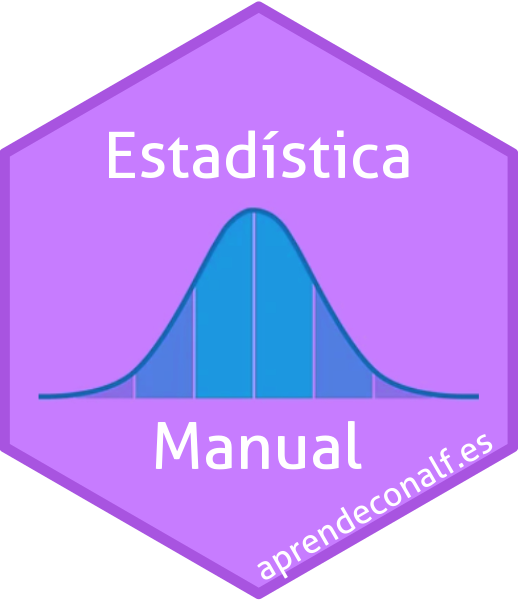
\includegraphics[width=0.4\textwidth]{img/logos/sticker.png}
\end{center}

\vfill

\begin{flushleft}
\begin{tabular}{ll}

\includegraphics[width=0.1\textwidth]{img/logos/aprendeconalf.png} & \parbox[b]{5cm}{\Large\textsf{Alfredo
Sánchez
Alberca}\\ \textsf{asalber@ceu.es} \\ \textsf{https://aprendeconalf.es}}
\end{tabular}
\end{flushleft}
\end{titlepage}
\renewcommand*\contentsname{Indice de contenidos}
{
\hypersetup{linkcolor=}
\setcounter{tocdepth}{2}
\tableofcontents
}
\bookmarksetup{startatroot}

\chapter*{Prefacio}\label{prefacio}
\addcontentsline{toc}{chapter}{Prefacio}

\markboth{Prefacio}{Prefacio}

¡Bienvenida/os al manual de Estadística!

Este libro es una introducción a la Estadística básica y el cálculo de
probabilidades para alumnos de grados de ciencias e ingenierías.

Este libro se complementa con los siguientes recursos:

\begin{itemize}
\tightlist
\item
  \href{https://aprendeconalf.es/estadistica-ejercicios/}{Colección de
  problemas resueltos}
\item
  \href{https://aprendeconalf.es/estadistica-practicas-r/}{Prácticas de
  Estadística con R}
\end{itemize}

\section*{Licencia}\label{licencia}
\addcontentsline{toc}{section}{Licencia}

\markright{Licencia}

Esta obra está bajo una licencia Reconocimiento -- No comercial --
Compartir bajo la misma licencia 3.0 España de Creative Commons. Para
ver una copia de esta licencia, visite
\url{https://creativecommons.org/licenses/by-nc-sa/3.0/es/}.

Con esta licencia eres libre de:

\begin{itemize}
\tightlist
\item
  Copiar, distribuir y mostrar este trabajo.
\item
  Realizar modificaciones de este trabajo.
\end{itemize}

Bajo las siguientes condiciones:

\begin{itemize}
\item
  **Reconocimiento Debe reconocer los créditos de la obra de la manera
  especificada por el autor o el licenciador (pero no de una manera que
  sugiera que tiene su apoyo o apoyan el uso que hace de su obra).
\item
  **No comercial No puede utilizar esta obra para fines comerciales.
\item
  **Compartir bajo la misma licencia Si altera o transforma esta obra, o
  genera una obra derivada, sólo puede distribuir la obra generada bajo
  una licencia idéntica a ésta.
\end{itemize}

Al reutilizar o distribuir la obra, tiene que dejar bien claro los
términos de la licencia de esta obra.

Estas condiciones pueden no aplicarse si se obtiene el permiso del
titular de los derechos de autor.

Nada en esta licencia menoscaba o restringe los derechos morales del
autor.

\bookmarksetup{startatroot}

\chapter{Introducción a la
Estadística}\label{introducciuxf3n-a-la-estaduxedstica}

\section{La estadística como herramienta
científica}\label{la-estaduxedstica-como-herramienta-cientuxedfica}

\subsection{¿Qué es la estadística?}\label{quuxe9-es-la-estaduxedstica}

\begin{definition}[Estadística]\protect\hypertarget{def-estadistica}{}\label{def-estadistica}

La \emph{estadística} es una rama de las matemáticas que se encarga de
la recogida, análisis e interpretación de datos.

\end{definition}

El papel de la Estadística es extraer información de los datos para
adquirir el conocimiento necesario para tomar decisiones.

\begin{figure}[H]

{\centering 
\includegraphics{img/introduccion/proposito_estadistica.png}

}

\caption{Propósito de la Estadística}

\end{figure}%

La estadística es imprescindible en cualquier disciplina científica o
técnica donde se manejen datos, especialmente si son grandes volúmenes
de datos, como por ejemplo en Física, Química, Medicina, Psicología,
Economía o Ciencias Sociales.

Pero, \emph{¿por qué es necesaria la Estadística?}

\subsection{La variabilidad de nuestro
mundo}\label{la-variabilidad-de-nuestro-mundo}

El científico trata de estudiar el mundo que le rodea; un mundo que está
lleno de variaciones que dificultan la determinación del comportamiento
de las cosas.

La estadística actúa como disciplina puente entre la realidad del mundo
y los modelos matemáticos que tratan de explicarla, proporcionando una
metodología para evaluar las discrepancias entre la realidad y los
modelos teóricos.

Esto la convierte en una herramienta indispensable en las ciencias
aplicadas que requieran el análisis de datos y el diseño de
experimentos.

\section{Población y muestra}\label{poblaciuxf3n-y-muestra}

\subsection{Población estadística}\label{poblaciuxf3n-estaduxedstica}

\begin{definition}[Población]\protect\hypertarget{def-poblacion}{}\label{def-poblacion}

Una \emph{población} es un conjunto de elementos definido por una o más
características que tienen todos los elementos, y sólo ellos. Cada
elemento de la población se llama \emph{individuo}.

\end{definition}

\begin{definition}[Tamaño
poblacional]\protect\hypertarget{def-tamaño-poblacional}{}\label{def-tamaño-poblacional}

El número de individuos de una población se conoce como \emph{tamaño
poblacional} y se representa como \(N\).

\end{definition}

\begin{example}[]\protect\hypertarget{exm-tamaño-poblacional}{}\label{exm-tamaño-poblacional}

En unas elecciones generales a la presidencia del gobierno, la población
serían todos los individuos del estado con derecho a voto. En el estudio
de una enfermedad, la población sería todas las personas que tienen la
enfermedad. Y en un proceso de control de calidad en la fabricación de
un fármaco, la población estaría formada por todos los fármacos que se
producen en la fábrica.

\end{example}

A veces, no todos los elementos de la población están accesibles para su
estudio. Entonces se distingue entre:

\begin{itemize}
\tightlist
\item
  \textbf{Población Teórica}: Conjunto de elementos a los que se quiere
  extrapolar los resultados del estudio.
\item
  \textbf{Población Estudiada}: Conjunto de elementos realmente
  accesibles en el estudio.
\end{itemize}

\begin{example}[]\protect\hypertarget{exm-poblacion-teorica-observada}{}\label{exm-poblacion-teorica-observada}

En el caso del estudio de una enfermedad, la población teórica sería
todas las personas que contraigan la enfermedad, incluso si aún no han
nacido, mientras que la población estudiada se limitaría al número de
personas enfermas que realmente podemos estudiar (obsérvese que incluso
quedarían fuera las personas enfermas pero de las que no podemos
conseguir información).

\end{example}

\subsection{Inconvenientes en el estudio de la
población}\label{inconvenientes-en-el-estudio-de-la-poblaciuxf3n}

El científico estudia un determinado fenómeno en una población para
comprenderlo, obtener conocimiento sobre el mismo, y así poder
controlarlo. Pero, para tener un conocimiento completo de la población
\emph{es necesario estudiar todos los individuos de la misma}. Sin
embargo, esto no siempre es posible por distintos motivos:

\begin{itemize}
\tightlist
\item
  El tamaño de la población es infinito, o bien es finito pero demasiado
  grande.
\item
  Las pruebas a que se someten los individuos son destructivas.
\item
  El coste, tanto de dinero como de tiempo, que supondría estudiar a
  todos los individuos es excesivo.
\end{itemize}

\subsection{Muestra estadística}\label{muestra-estaduxedstica}

Cuando no es posible o conveniente estudiar todos los individuos de la
población, se estudia sólo una parte de la misma.

\begin{definition}[Muestra]\protect\hypertarget{def-muestra}{}\label{def-muestra}

Una \emph{muestra} es un subconjunto de la población.

\end{definition}

\begin{definition}[Tamaño
muestral]\protect\hypertarget{def-tamaño-muestral}{}\label{def-tamaño-muestral}

Al número de individuos que componen la muestra se le llama \emph{tamaño
muestral} y se representa por \(n\).

\end{definition}

Habitualmente, el estudio de una población se realiza a partir de
muestras extraídas de dicha población.

Generalmente, el estudio de la muestra sólo aporta conocimiento
aproximado de la población. Pero en muchos casos es \emph{suficiente}.

\subsection{Determinación del tamaño
muestral}\label{determinaciuxf3n-del-tamauxf1o-muestral}

Una de las preguntas más interesantes que surge inmediatamente es:
\emph{¿cuántos individuos es necesario tomar en la muestra para tener un
conocimiento aproximado pero suficiente de la población?}

La respuesta depende de varios factores, como la variabilidad de la
población o la fiabilidad deseada para las extrapolaciones que se hagan
hacia la población.

Por desgracia no se podrá responder hasta casi el final del curso, pero
en general, cuantos más individuos haya en la muestra, más fiables serán
las conclusiones sobre la población, pero también será más lento y
costoso el estudio.

\begin{example}[]\protect\hypertarget{exm-tamaño-muestral-suficiente}{}\label{exm-tamaño-muestral-suficiente}

Para entender a qué nos referimos cuando hablamos de un tamaño muestral
suficiente para comprender lo que ocurre en la población, podemos
utilizar el siguiente símil en que se trata de comprender el motivo que
representa una fotografía.

Una fotografía digital está formada por multitud de pequeños puntitos
llamados pixels que se dispone en una enorme tabla de filas y columnas
(cuantas más filas y columnas haya se habla de que la foto tiene más
resolución). Aquí la población estaría formada por todos y cada uno de
los píxeles que forman la foto. Por otro lado cada pixel tiene un color
y es la variedad de colores a lo largo de los pixels la que permite
formar la imagen de la fotografía.

\emph{¿Cuántos píxeles debemos tomar en una muestra para averiguar la
imagen de la foto?}

La respuesta depende de la variabilidad de colores en la foto. Si todos
los pixels de la foto son del mismo color, entonces un sólo pixel basta
para desvelar la imagen. Pero, si la foto tiene mucha variabilidad de
colores, necesitaremos muchos más pixels en la muestra para descubrir el
motivo de la foto.

La imagen siguiente contiene una muestra pequeña de píxeles de una foto.
¿Puedes averiguar el motivo de a foto?

\begin{figure}[H]

{\centering 
\includegraphics{img/introduccion/muestra_molinos1.jpg}

}

\caption{Muestra pequeña de píxeles de una foto.}

\end{figure}%

\emph{¡Con una muestra pequeña es difícil averiguar el contenido de la
imagen!}

Seguramente no has podido averiguar el motivo de la fotografía, porque
en este caso el número de píxeles que hemos tomado en la muestra es
insuficiente para comprender toda la variabilidad de colores que hay en
la foto.

La siguiente imagen contiene una muestra mayor de píxeles. ¿Eres capaz
de adivinar el motivo de la foto ahora?

\begin{figure}[H]

{\centering 
\includegraphics{img/introduccion/muestra_molinos2.jpg}

}

\caption{Muestra mayor de píxeles de una foto.}

\end{figure}%

\emph{¡Con una muestra mayor es posible desvelar el motivo de la foto!}

Y aquí está la población completa.

\begin{figure}[H]

{\centering 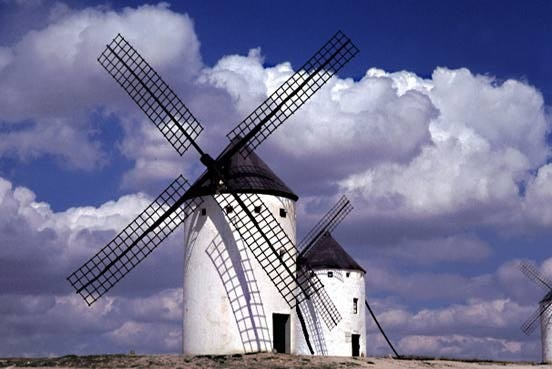
\includegraphics{img/introduccion/muestra_molinos3.jpg}

}

\caption{Población de píxeles de una foto.}

\end{figure}%

Lo importante es que \emph{¡No es necesario conocer todos los píxeles
para averiguar la imagen!}

\end{example}

\subsection{Tipos de razonamiento}\label{tipos-de-razonamiento}

Así pues, habitualmente realizaremos el estudio de la población a partir
de muestras y luego trataremos de extrapolar lo observado en la muestra
al resto de la población. A este tipo de razonamiento que saca
conclusiones desde la muestra hacia la población se le conoce como
\emph{razonamiento inductivo}.

\begin{figure}[H]

{\centering 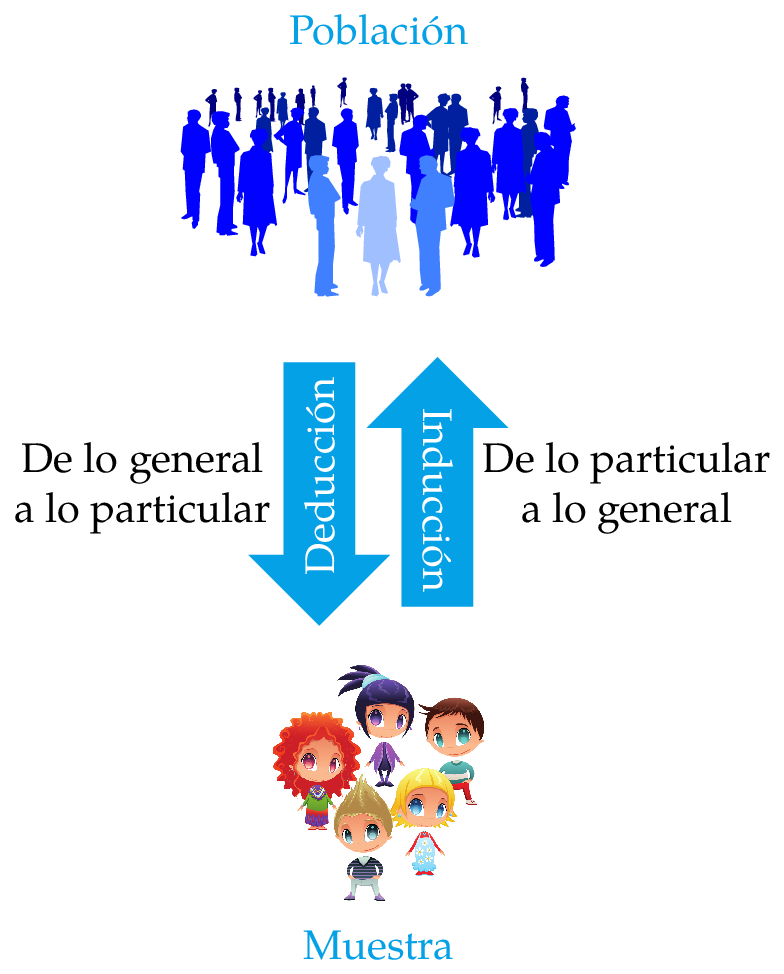
\includegraphics{img/introduccion/tipos_razonamiento.png}

}

\caption{Tipos de razonamiento.}

\end{figure}%

\begin{itemize}
\item
  \emph{Características de la deducción}: Si las premisas son ciertas,
  garantiza la certeza de las conclusiones (es decir, si algo se cumple
  en la población, también se cumple en la muestra). Sin embargo,
  \emph{¡no aporta conocimiento nuevo!}
\item
  \emph{Características de la inducción}: No garantiza la certeza de las
  conclusiones (si algo se cumple en la muestra, puede que no se cumpla
  en la población, así que ¡cuidado con las extrapolaciones!), pero
  \emph{¡es la única forma de generar conocimiento nuevo!}
\end{itemize}

La estadística se apoya fundamentalmente en el razonamiento inductivo ya
que utiliza la información obtenida a partir de muestras para sacar
conclusiones sobre las poblaciones. A diferencia del razonamiento
deductivo que va de lo general a lo particular, o en nuestro caso de la
población a la muestra, el razonamiento inductivo no garantiza la
certeza de las conclusiones, por lo que debemos ser cuidadosos a la hora
de generalizar sobre la población lo observado en al muestra, ya que si
la muestra no es representativa de la población o contiene sesgos, las
conclusiones pueden ser erróneas.

\section{Muestreo}\label{muestreo}

\begin{definition}[Muestreo]\protect\hypertarget{def-muestreo}{}\label{def-muestreo}

El proceso de selección de los elementos que compondrán una muestra se
conoce como \emph{muestreo}.

\end{definition}

!{[}{]}(img/introduccion/muestreo.svg'' alt=``Muestreo''
width=``500px''\textgreater{}

Para que una muestra refleje información fidedigna sobre la población
global debe ser representativa de la misma, lo que significa que debe
reproducir a pequeña escala la variabilidad de la población.

\emph{El objetivo es obtener una muestra representativa de la
población.}

\subsection{Modalidades de muestreo}\label{modalidades-de-muestreo}

Existen muchas técnicas de muestreo pero se pueden agrupar en dos
categorías:

\begin{itemize}
\item
  \textbf{Muestreo Aleatorio}: Elección aleatoria de los individuos de
  la muestra. Todos tienen la misma probabilidad de ser elegidos
  (\emph{equiprobabilidad}).
\item
  \textbf{Muestreo No Aleatorio}: Los individuos se eligen de forma no
  aleatoria. Algunos individuos tienen más probabilidad de ser
  seleccionados que otros.
\end{itemize}

Sólo las técnicas aleatorias evitan el sesgo de selección, y por tanto,
garantizan la representatividad de la muestra extraída, y en
consecuencia la validez de las conclusiones.

Las técnicas no aleatorias no sirven para hacer generalizaciones, ya que
no garantizan la representatividad de la muestra. Sin embargo, son menos
costosas y pueden utilizarse en estudios exploratorios.

\subsection{Muestreo aleatorio simple}\label{muestreo-aleatorio-simple}

Dentro de las modalidades de muestreo aleatorio, el tipo más conocido es
el \emph{muestreo aleatorio simple}, caracterizado por:

\begin{itemize}
\tightlist
\item
  Todos los individuos de la población tienen la misma probabilidad de
  ser elegidos para la muestra.
\item
  La selección de individuos es con reemplazamiento, es decir, cada
  individuo seleccionado es devuelto a la población antes de seleccionar
  al siguiente (y por tanto no se altera la población de partida).
\item
  Las sucesivas selecciones de un individuo son independientes.
\end{itemize}

La única forma de realizar un muestreo aleatorio es asignar un número a
cada individuo de la población (\emph{censo}) y realizar un sorteo
aleatorio.

\subsection{Variables estadísticas}\label{variables-estaduxedsticas}

Todo estudio estadístico comienza por la identificación de las
características que interesa estudiar en la población y que se medirán
en los individuos de la muestra.

\begin{definition}[Variable
estadística]\protect\hypertarget{def-variable-estadistica}{}\label{def-variable-estadistica}

Una \emph{variable estadística} es una propiedad o característica medida
en los individuos de la población.

Los \emph{datos} son los valores observados en las variables
estadísticas.

\end{definition}

\begin{figure}[H]

{\centering 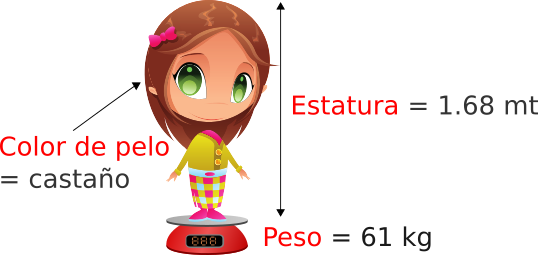
\includegraphics{img/introduccion/variables_estadisticas.png}

}

\caption{Variables estadísticas.}

\end{figure}%

Estas características pueden ser de distintos tipos de acuerdo a su
naturaleza y su escala:

\begin{itemize}
\item
  \textbf{Variables cualitativas o atributos}: Miden cualidades no
  numéricas. Pueden ser:

  \begin{itemize}
  \item
    \textbf{Nominales}: No existe un orden entre las categorías.\\
    Ejemplo: El color de pelo o el sexo.
  \item
    \textbf{Ordinales}: Existe un orden entre las categorías. Ejemplo:
    El nivel de estudios o la gravedad de una enfermedad.
  \end{itemize}
\item
  \textbf{Variables cuantitativas}: Miden cantidades numéricas. Pueden
  ser:

  \begin{itemize}
  \item
    \textbf{Discretas}: Toman valores numéricos aislados (habitualmente
    números enteros).\\
    Ejemplo: El número de hijos o el número de coches en una familia.
  \item
    \textbf{Continuas}: Pueden tomar cualquier valor en un intervalo
    real.\\
    Ejemplo: El peso o la estatura.
  \end{itemize}
\end{itemize}

Las variables cualitativas y discretas se conocen también con
\emph{variables categóricas} y sus valores \emph{categorías}.

\begin{figure}[H]

{\centering 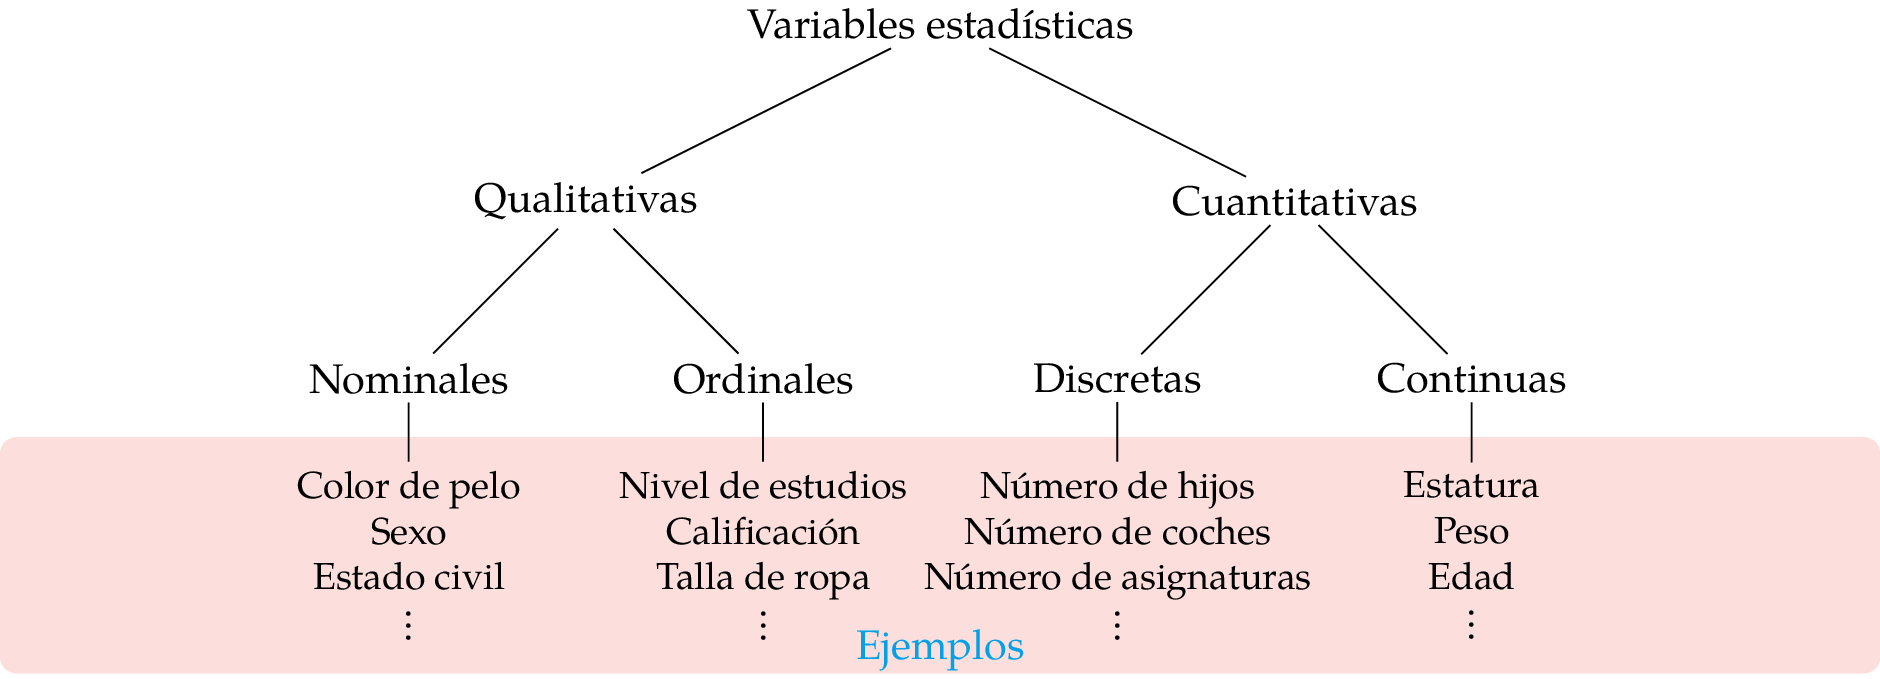
\includegraphics{img/introduccion/tipos_variables.png}

}

\caption{Tipos de variables estadísticas.}

\end{figure}%

\subsubsection{Elección del tipo de variable más
apropiado}\label{elecciuxf3n-del-tipo-de-variable-muxe1s-apropiado}

En ocasiones una característica puede medirse mediante variables de
distinto tipo.

\begin{example}[]\protect\hypertarget{exm-eleccion-tipos-variables}{}\label{exm-eleccion-tipos-variables}

Si una persona fuma o no podría medirse de diferentes formas:

\begin{itemize}
\item
  Fuma: si/no. (Nominal)
\item
  Nivel de fumador: No fuma / ocasional / moderado / bastante /
  empedernido. (Ordinal)
\item
  Número de cigarros diarios: 0,1,2,\ldots{} (Discreta)
\end{itemize}

\end{example}

En estos casos es preferible usar variables cuantitativas a
cualitativas. Dentro de las cuantitativas es preferible usar las
continuas a las discretas y dentro de las cualitativas es preferible
usar ordinales a nominales pues aportan más información.

\begin{figure}[H]

{\centering 
\includegraphics{img/introduccion/informacion_variables.png}

}

\caption{Cantidad de información de los tipos de variables
estadísticas.}

\end{figure}%

De acuerdo al papel que juegan en el estudio las variables también
pueden clasificarse como:

\begin{itemize}
\item
  \textbf{Variables independientes}: Variables que supuestamente no
  dependen de otras variables en el estudio. Habitualmente son las
  variables manipuladas en el experimento para ver su efecto en las
  variables dependientes. Se conocen también como \emph{variables
  predictivas}.
\item
  \textbf{Variables dependientes}: Variables que supuestamente dependen
  de otras variables en el estudio. No son manipuladas en el experimento
  y también se conocen como \emph{variables respuesta}.
\end{itemize}

\begin{example}[]\protect\hypertarget{exm-variables-dependientes-independientes}{}\label{exm-variables-dependientes-independientes}

En un estudio sobre el rendimiento de los alumnos de un curso, la
inteligencia de los alumnos y el número de horas de estudio diarias
serían variables independientes y la nota del curso sería una variable
dependiente.

\end{example}

\subsection{Tipos de estudios
estadísticos}\label{tipos-de-estudios-estaduxedsticos}

Dependiendo de si se manipulan las variables independientes existen dos
tipos de estudios:

\begin{itemize}
\tightlist
\item
  \textbf{Experimentales}: Cuando las variables independientes son
  manipuladas para ver el efecto que producen en las variables
  dependientes.
\end{itemize}

\begin{example}[]\protect\hypertarget{exm-estudios-experimentales}{}\label{exm-estudios-experimentales}

En un estudio sobre el rendimiento de los estudiantes en un test, el
profesor manipula la metodología de estudio para crear dos o más grupos
con metodologías de estudio distintas.

\end{example}

\begin{itemize}
\tightlist
\item
  \textbf{No experimentales}: Cuando las variables independientes no son
  manipuladas. Esto no significa que sea imposible hacerlo, sino que es
  difícil o poco ético hacerlo.
\end{itemize}

\begin{example}[]\protect\hypertarget{exm-estudios-no-experimentales}{}\label{exm-estudios-no-experimentales}

En un estudio un investigador puede estar interesado en el efecto de
fumar sobre el cáncer de pulmón. Aunque es posible, no sería ético
pedirle a los pacientes que fumasen para ver el efecto que tiene sobre
sus pulmones. En este caso, el investigador podría estudiar dos grupos
de pacientes, uno con cáncer de pulmón y otro sin cáncer, y observar en
cada grupo cuántos fuman o no.

\end{example}

Los estudios experimentales permiten identificar causas y efectos entre
las variables del estudio, mientras que los no experimentales sólo
permiten identificar relaciones de asociación entre las variables.

\subsection{La tabla de datos}\label{la-tabla-de-datos}

Las variables a estudiar se medirán en cada uno de los individuos de la
muestra, obteniendo un conjunto de datos que suele organizarse en forma
de matriz que se conoce como tabla de datos\_.

En esta tabla cada columna contiene la información de una variable y
cada fila la información de un individuo.

\begin{example}[]\protect\hypertarget{exm-tabla-datos}{}\label{exm-tabla-datos}

La siguiente tabla contiene información de las variables Nombre, Edad,
Sexo, Peso y Altura de una muestra de 6 personas.

\begin{longtable}[]{@{}lcccc@{}}
\toprule\noalign{}
Nombre & Edad & Sexo & Peso(Kg) & Altura(cm) \\
\midrule\noalign{}
\endhead
\bottomrule\noalign{}
\endlastfoot
José Luis Martínez & 18 & H & 85 & 179 \\
Rosa Díaz & 32 & M & 65 & 173 \\
Javier García & 24 & H & 71 & 181 \\
Carmen López & 35 & M & 65 & 170 \\
Marisa López & 46 & M & 51 & 158 \\
Antonio Ruiz & 68 & H & 66 & 174 \\
\end{longtable}

\end{example}

\subsection{Fases del análisis
estadístico}\label{fases-del-anuxe1lisis-estaduxedstico}

Normalmente un estudio estadístico pasa por las siguientes etapas:

\begin{enumerate}
\def\labelenumi{\arabic{enumi}.}
\item
  El estudio comienza por el diseño previo del mismo en el que se
  establezcan los objetivos del mismo, la población, las variables que
  se medirán y el tamaño muestral requerido.
\item
  A continuación se seleccionará una muestra representativa del tamaño
  establecido y se medirán las variables en los individuos de la muestra
  obteniendo la tabla de datos. De esto se encarga el \emph{Muestreo}.
\item
  El siguiente paso consiste en describir y resumir la información que
  contiene la muestra. De esto se encarga la \emph{Estadística
  Descriptiva}.
\item
  La información obtenida es proyectada sobre un modelo matemático que
  intenta explicar el comportamiento de la población y el modelo se
  valida. De todo esto se encarga la \emph{Estadística Inferencial}.
\item
  Finalmente, el modelo validado nos permite hacer predicciones y sacar
  conclusiones sobre la población de partida con cierta confianza.
\end{enumerate}

\subsubsection{El ciclo estadístico}\label{el-ciclo-estaduxedstico}

\begin{figure}[H]

{\centering 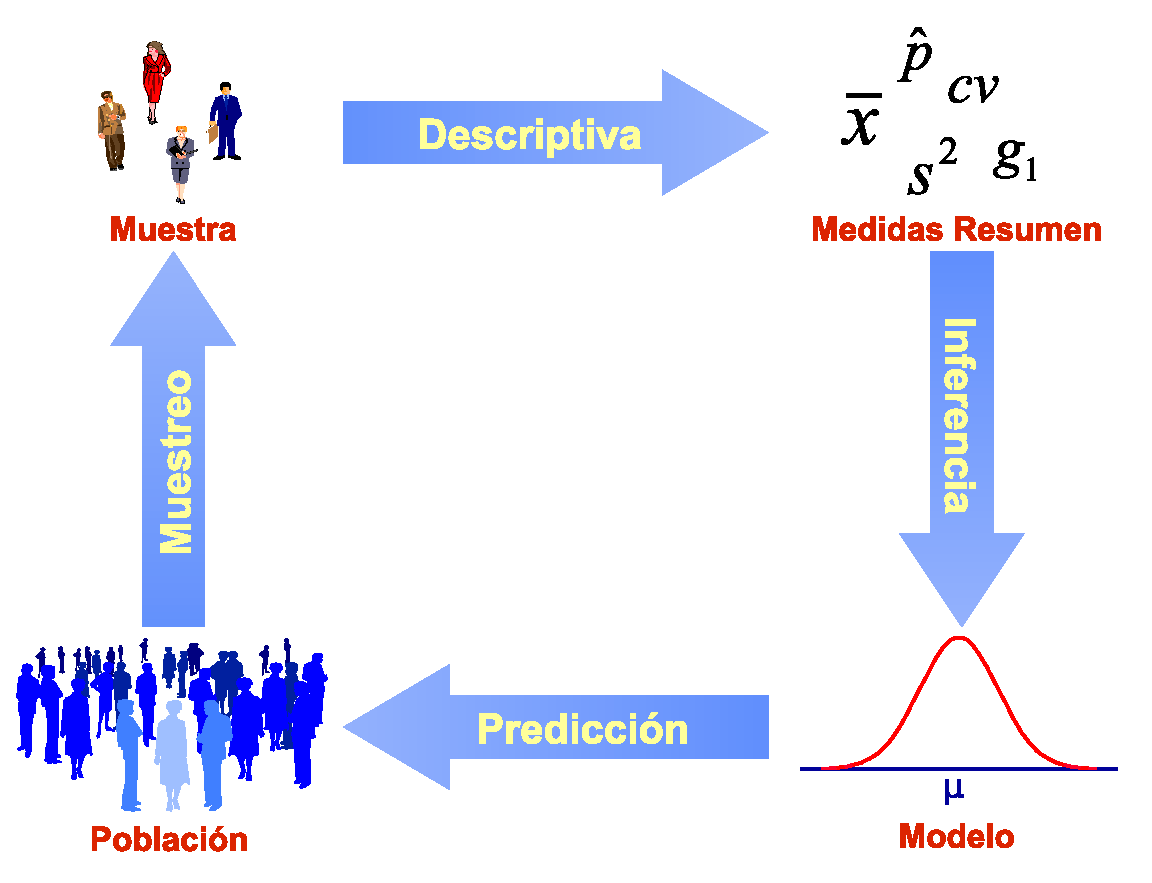
\includegraphics{img/introduccion/ciclo_estadistico.eps}

}

\caption{El ciclo estadístico.}

\end{figure}%

\bookmarksetup{startatroot}

\chapter{Estadística Descriptiva}\label{estaduxedstica-descriptiva}

La estadística descriptiva es la parte de la estadística encargada de
representar, analizar y resumir la información contenida en la muestra.

Tras el proceso de muestreo, es la siguiente etapa de todo estudio
estadístico y suele consistir en:

\begin{enumerate}
\def\labelenumi{\arabic{enumi}.}
\item
  Clasificar, agrupar y ordenar los datos de la muestra.
\item
  Tabular y representar gráficamente los datos de acuerdo a sus
  frecuencias.
\item
  Calcular medidas que resuman la información que contiene la muestra
  (\emph{estadísticos muestrales}).
\end{enumerate}

\begin{tcolorbox}[enhanced jigsaw, title=\textcolor{quarto-callout-note-color}{\faInfo}\hspace{0.5em}{Interpretación}, coltitle=black, colframe=quarto-callout-note-color-frame, opacitybacktitle=0.6, toprule=.15mm, breakable, opacityback=0, colbacktitle=quarto-callout-note-color!10!white, colback=white, toptitle=1mm, rightrule=.15mm, bottomrule=.15mm, left=2mm, bottomtitle=1mm, titlerule=0mm, arc=.35mm, leftrule=.75mm]

No tiene poder inferencial, por lo que nunca deben sacarse conclusiones
sobre la población a partir de las medidas resumen que aporta la
Estadística Descriptiva.

\end{tcolorbox}

\section{Distribución de
frecuencias}\label{distribuciuxf3n-de-frecuencias}

El estudio de una variable estadística comienza por medir la variable en
los individuos de la muestra y clasificar los valores obtenidos.

Existen dos formas de clasificar estos valores:

\begin{itemize}
\item
  \textbf{Sin agrupar}: Ordenar todos los valores obtenidos en la
  muestra de menor a mayor. Se utiliza con atributos y variables
  discretas con pocos valores diferentes.
\item
  \textbf{Agrupados}: Agrupar los valores en clases (intervalos) y
  ordenar dichas clases de menor a mayor. Se utiliza con variables
  continuas y con variables discretas con muchos valores diferentes.
\end{itemize}

\subsection{Clasificación de la
muestra}\label{clasificaciuxf3n-de-la-muestra}

Consiste colocar juntos los valores iguales y ordenarlos si existe un
orden entre ellos.

\begin{figure}[H]

{\centering 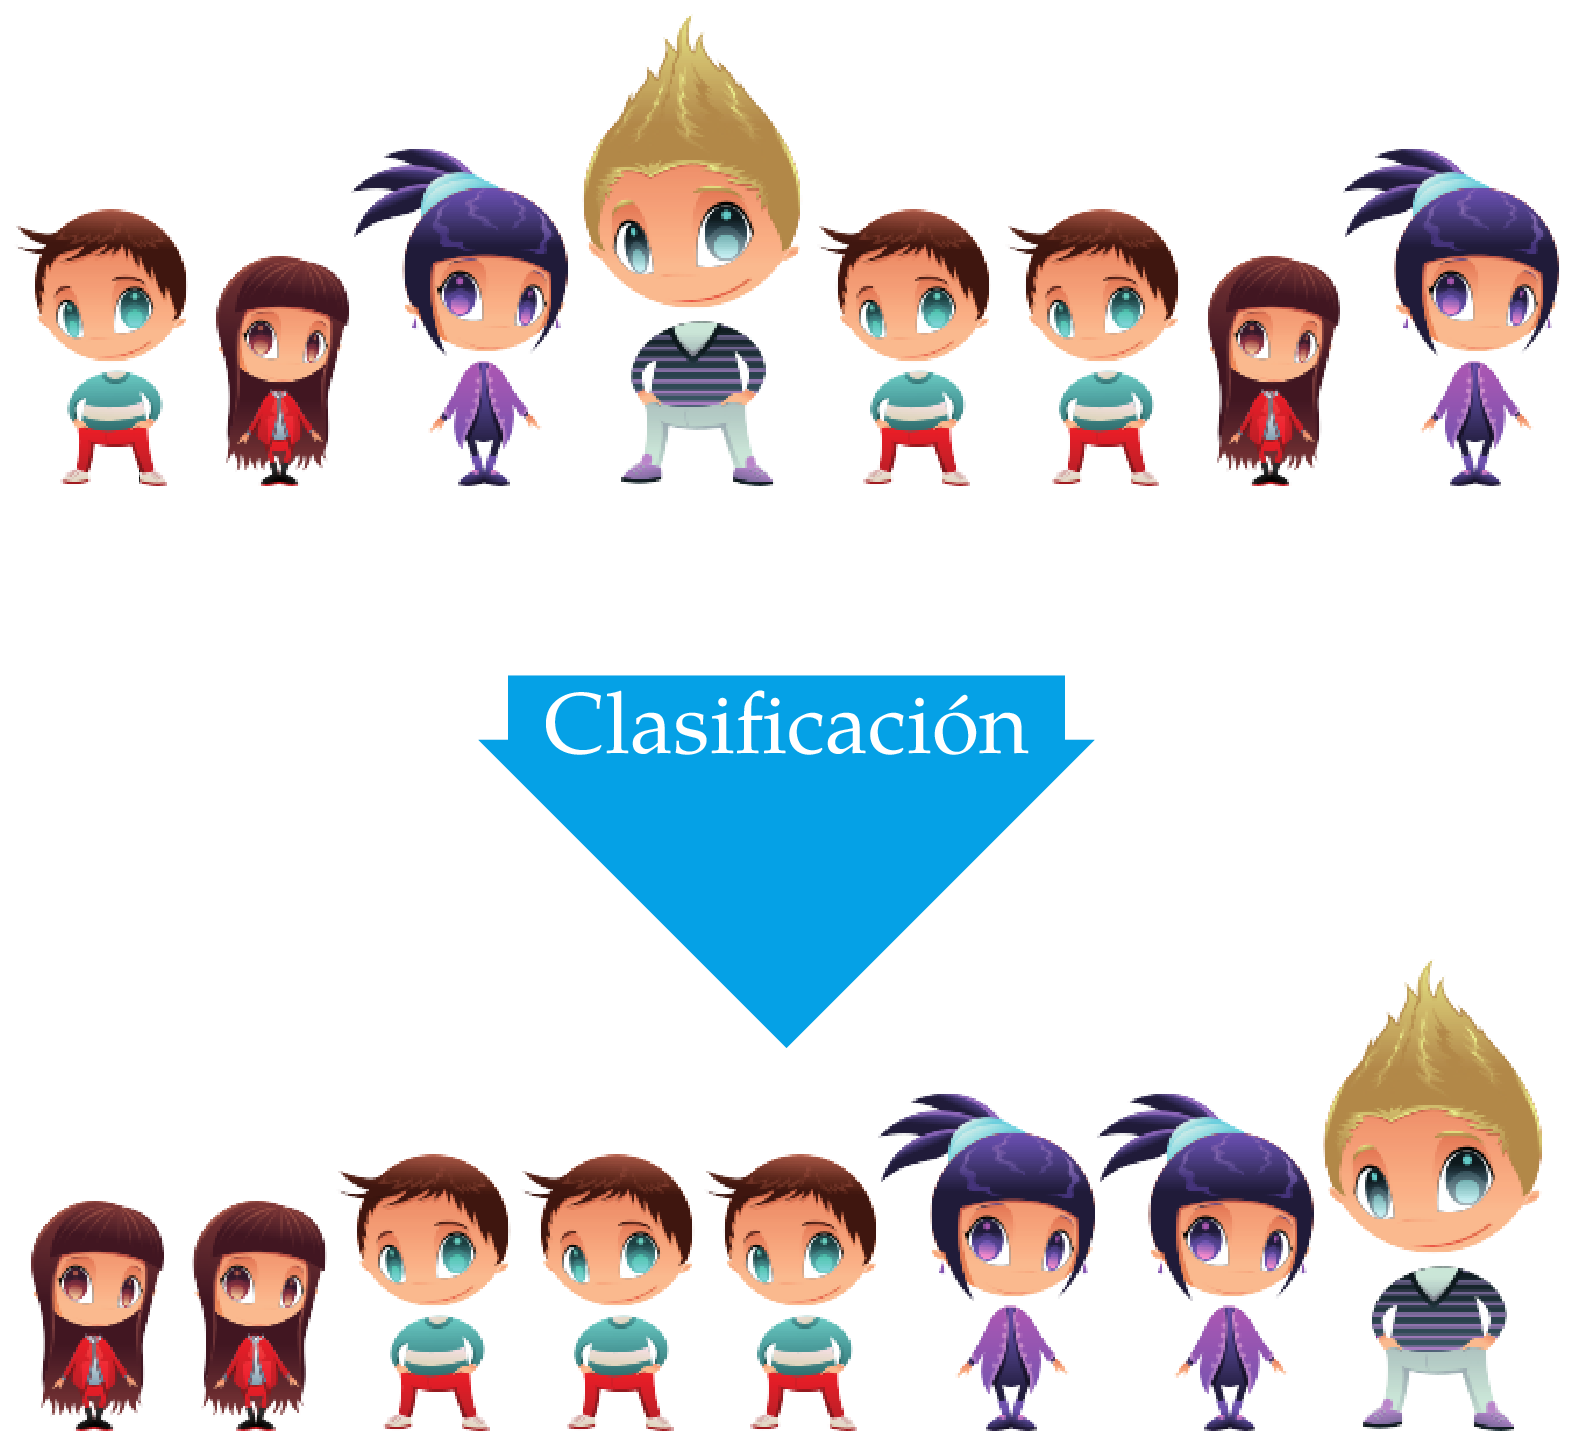
\includegraphics{img/descriptiva/clasificacion_muestra.png}

}

\caption{Clasificación de la muestra.}

\end{figure}%

\subsection{Recuento de frecuencias}\label{recuento-de-frecuencias}

\begin{figure}[H]

{\centering 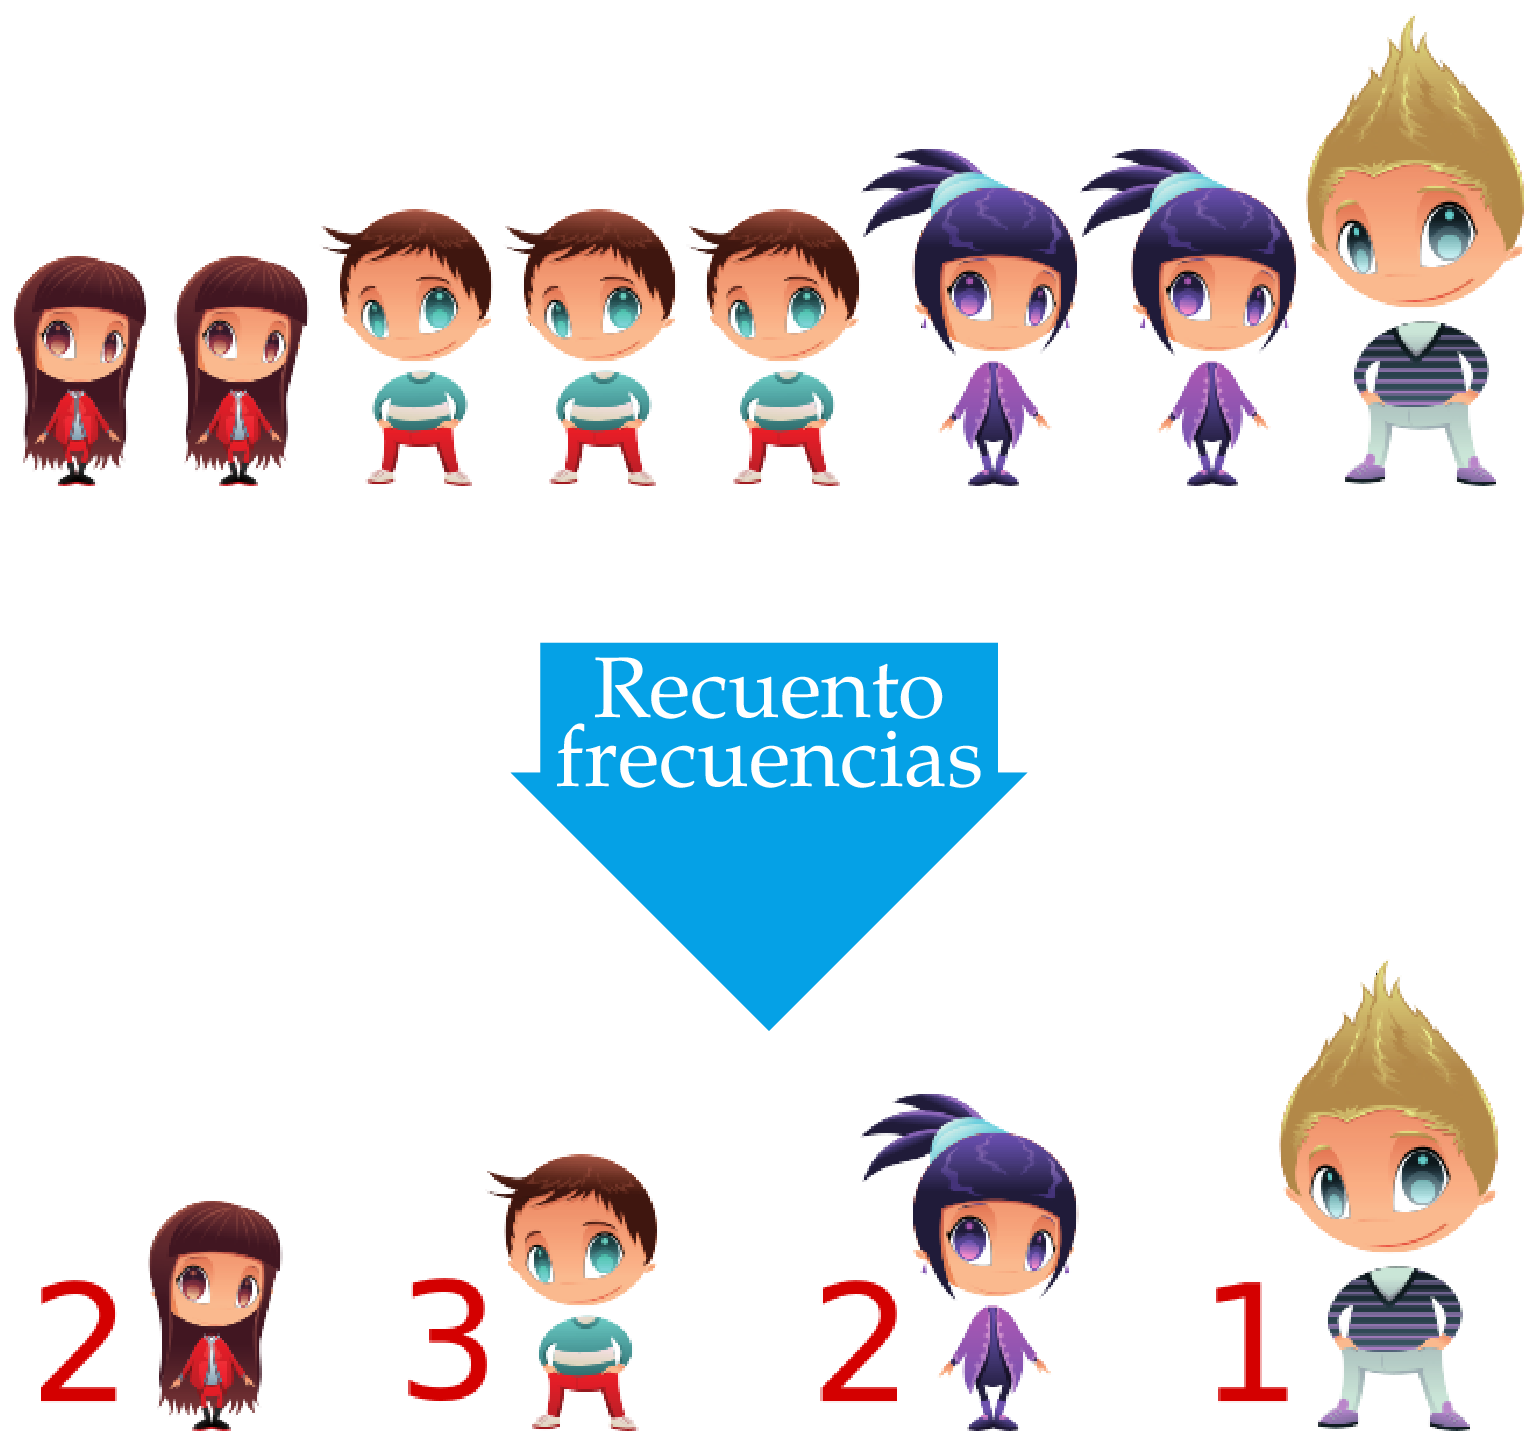
\includegraphics{img/descriptiva/recuento_frecuencias.png}

}

\caption{Recuento de frecuencias}

\end{figure}%

\section{Frecuencias muestrales}\label{frecuencias-muestrales}

\begin{definition}[Frecuencias
muestrales]\protect\hypertarget{def-frecuencias-muestrales}{}\label{def-frecuencias-muestrales}

Dada una muestra de tamaño \(n\) de una variable \(X\), para cada valor
de la variable \(x_i\) observado en la muestra, se define

\begin{itemize}
\tightlist
\item
  \textbf{Frecuencia Absoluta \(n_i\)}: Es el número de veces que el
  valor \(x_i\) aparece en la muestra.
\item
  \textbf{Frecuencia Relativa \(f_i\)}: Es la proporción de veces que el
  valor \(x_i\) aparece en la muestra. \[f_i = \frac{n_i}{n}\]
\item
  \textbf{Frecuencia Absoluta Acumulada \(N_i\)}: Es el número de
  valores en la muestra menores o iguales que \(x_i\).
  \[N_i = n_1 + \cdots + n_i = N_{i-1}+n_i\]
\item
  \textbf{Frecuencia Relativa Acumulada \(F_i\)}: Es la proporción de
  valores en la muestra menores o iguales que \(x_i\).
  \[F_i = \frac{N_i}{n}\]
\end{itemize}

\end{definition}

\subsection{Tabla de frecuencias}\label{tabla-de-frecuencias}

Al conjunto de valores observados en la muestra junto a sus respectivas
frecuencias se le denomina \textbf{distribución de frecuencias} y suele
representarse mediante una \textbf{tabla de frecuencias}.

\begin{longtable}[]{@{}
  >{\centering\arraybackslash}p{(\columnwidth - 8\tabcolsep) * \real{0.1273}}
  >{\centering\arraybackslash}p{(\columnwidth - 8\tabcolsep) * \real{0.1727}}
  >{\centering\arraybackslash}p{(\columnwidth - 8\tabcolsep) * \real{0.1727}}
  >{\centering\arraybackslash}p{(\columnwidth - 8\tabcolsep) * \real{0.2636}}
  >{\centering\arraybackslash}p{(\columnwidth - 8\tabcolsep) * \real{0.2636}}@{}}
\toprule\noalign{}
\begin{minipage}[b]{\linewidth}\centering
Valores de \(X\)
\end{minipage} & \begin{minipage}[b]{\linewidth}\centering
Frecuencia Absoluta
\end{minipage} & \begin{minipage}[b]{\linewidth}\centering
Frecuencia Relativa
\end{minipage} & \begin{minipage}[b]{\linewidth}\centering
Frecuencia Absoluta Acumulada
\end{minipage} & \begin{minipage}[b]{\linewidth}\centering
Frecuencia Relativa Acumulada
\end{minipage} \\
\midrule\noalign{}
\endhead
\bottomrule\noalign{}
\endlastfoot
\(x_1\) & \(n_1\) & \(f_1\) & \(N_1\) & \(F_1\) \\
\(\vdots\) & \(\vdots\) & \(\vdots\) & \(\vdots\) & \(\vdots\) \\
\(x_i\) & \(n_i\) & \(f_i\) & \(N_i\) & \(F_i\) \\
\(\vdots\) & \(\vdots\) & \(\vdots\) & \(\vdots\) & \(\vdots\) \\
\(x_k\) & \(n_k\) & \(f_k\) & \(N_k\) & \(F_k\) \\
\end{longtable}

\begin{example}[Variable cuantitativa y datos no
agrupados]\protect\hypertarget{exm-tabla-frecuencias-datos-no-agrupados}{}\label{exm-tabla-frecuencias-datos-no-agrupados}

El número de hijos en 25 familias es:

1, 2, 4, 2, 2, 2, 3, 2, 1, 1, 0, 2, 2, 0, 2, 2, 1, 2, 2, 3, 1, 2, 2, 1,
2

La tabla de frecuencias del número de hijos en esta muestra es

\[ 
\begin{array}{rrrrr}
\hline
x_i & n_i & f_i & N_i & F_i\\
\hline
0 & 2 & 0.08 & 2 & 0.08\\
1 & 6 & 0.24 & 8 & 0.32\\
2 & 14 & 0.56 & 22 & 0.88\\
3 & 2 & 0.08 & 24 & 0.96\\
4 & 1 & 0.04 & 25 & 1 \\
\hline
\sum & 25 & 1 \\
\hline
\end{array}
\]

\end{example}

\begin{example}[Variable cuantitativa y datos
agrupados]\protect\hypertarget{exm-tabla-frecuencias-datos-agrupados}{}\label{exm-tabla-frecuencias-datos-agrupados}

Se ha medido la estatura (en cm) de 30 universitarios obteniendo:

179, 173, 181, 170, 158, 174, 172, 166, 194, 185, 162, 187, 198, 177,
178, 165, 154, 188, 166, 171, 175, 182, 167, 169, 172, 186, 172, 176,
168, 187.

La tabla de frecuencias de la estatura en a esta muestra es

\[ 
\begin{array}{crrrr}
\hline
x_i & n_i & f_i & N_i & F_i\\
\hline
(150,160] & 2 & 0.07 & 2 & 0.07\\
(160,170] & 8 & 0.27 & 10 & 0.34\\
(170,180] & 11 & 0.36 & 21 & 0.70\\
(180,190] & 7 & 0.23 & 28 & 0.93\\
(190,200] & 2 & 0.07 & 30 & 1 \\
\hline
\sum & 30 & 1 \\
\hline
\end{array}
\]

\end{example}

\subsection{Construcción de clases}\label{construcciuxf3n-de-clases}

Cada intervalo de agrupación de datos se denomina \textbf{clase} y el
centro del intervalo se llama \textbf{marca de clase}.

A la hora de agrupar los datos en clases hay que tener en cuenta lo
siguiente:

\begin{itemize}
\tightlist
\item
  El número de intervalos no debe ser muy grande ni muy pequeño. Una
  regla orientativa es tomar un número de intervalos próximo a
  \(\sqrt{n}\) o \(\log_2(n)\).
\item
  Los intervalos no deben solaparse y deben cubrir todo el rango de
  valores. Es indiferente si se abren por la izquierda y se cierran por
  la derecha o al revés.
\item
  El valor más pequeño debe caer dentro del primer intervalo y el más
  grande dentro del último.
\end{itemize}

\begin{example}[Variable
cualitativa]\protect\hypertarget{exm-tabla-frecuencias-cualitativa}{}\label{exm-tabla-frecuencias-cualitativa}

Los grupos sanguíneos de una muestra de 30 personas son:

A, B, B, A, AB, 0, 0, A, B, B, A, A, A, A, AB, A, A, A, B, 0, B, B, B,
A, A, A, 0, A, AB, 0.

La tabla de frecuencias del grupo sanguíneo en esta muestra es

\[
\begin{array}{crr}
\hline
x_i & n_i & f_i \\
\hline
\mbox{0} & 5 & 0.16 \\
\mbox{A} & 14 & 0.47 \\
\mbox{B} & 8 & 0.27 \\
\mbox{AB} & 3 & 0.10 \\
\hline
\sum & 30 & 1 \\
\hline
\end{array}
\]

\end{example}

\begin{tcolorbox}[enhanced jigsaw, title=\textcolor{quarto-callout-warning-color}{\faExclamationTriangle}\hspace{0.5em}{Advertencia}, coltitle=black, colframe=quarto-callout-warning-color-frame, opacitybacktitle=0.6, toprule=.15mm, breakable, opacityback=0, colbacktitle=quarto-callout-warning-color!10!white, colback=white, toptitle=1mm, rightrule=.15mm, bottomrule=.15mm, left=2mm, bottomtitle=1mm, titlerule=0mm, arc=.35mm, leftrule=.75mm]

Obsérvese que en este caso las frecuencias acumuladas no tienen sentido
al no existir un orden entre los valores de la variable.

\end{tcolorbox}

\section{Representaciones gráficas}\label{representaciones-gruxe1ficas}

La tabla de frecuencias también suele representarse gráficamente.
Dependiendo del tipo de variable y de si se han agrupado o no los datos,
se utilizan distintos tipos de gráficos:

\begin{itemize}
\item
  Diagrama de barras
\item
  Histograma
\item
  Diagrama de líneas o polígonos.
\item
  Diagrama de sectores.
\end{itemize}

\subsection{Diagrama de barras}\label{diagrama-de-barras}

Un \textbf{diagrama de barras} consiste en un conjunto de barras, una
para cada valor o categoría de la variable, dibujadas sobre unos ejes
cartesianos.

Habitualmente los valores o categorías de la variable se representan en
eje \(X\), y las frecuencias en el eje \(Y\). Para cada valor o
categoría se dibuja una barra con la altura correspondiente a su
frecuencia. La anchura de la barra no es importante pero las barras
deben aparecer claramente separadas unas de otras.

Dependiendo del tipo de frecuencia representada en el eje \(Y\) se
tienen diferentes tipos de diagramas de barras.

En ocasiones se dibuja un polígono, conocido como \textbf{polígono de
frecuencias}, uniendo mediante segmentos los puntos más altos de cada
barra.

\begin{example}[]\protect\hypertarget{exm-diagrama-barras}{}\label{exm-diagrama-barras}

El diagrama de barras que aparece a continuación muestra la distribución
de frecuencias absolutas del número de hijos en la muestra anterior.

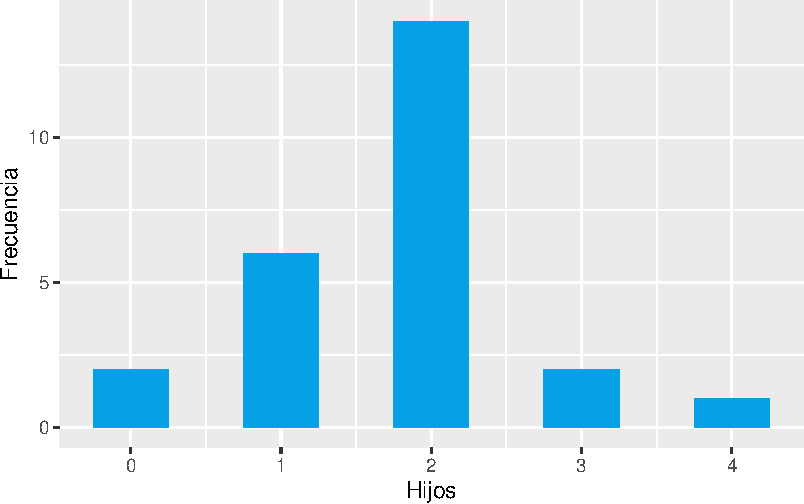
\includegraphics{02-estadistica-descriptiva_files/figure-pdf/diagrama-barras-1.pdf}

Y a continuación se muestra el polígono de frecuencias.

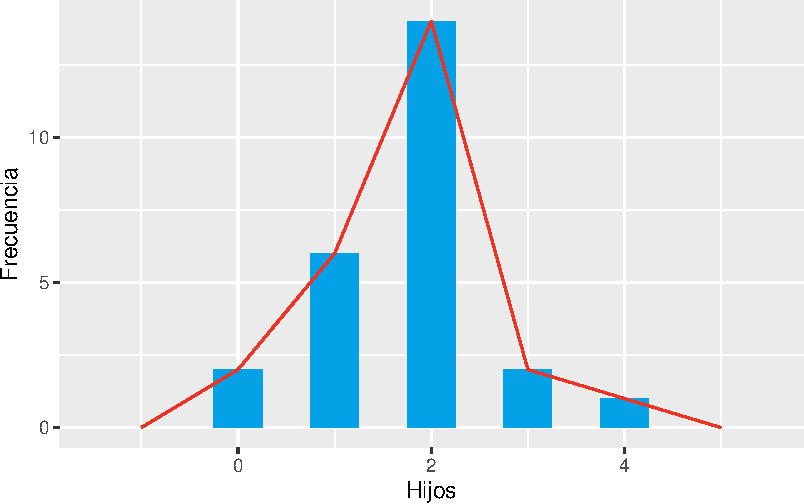
\includegraphics{02-estadistica-descriptiva_files/figure-pdf/poligono-frecuencias-absolutas-1.pdf}

El diagrama de barras que aparece a continuación muestra la distribución
de frecuencias relativas del número de hijos en la muestra anterior.

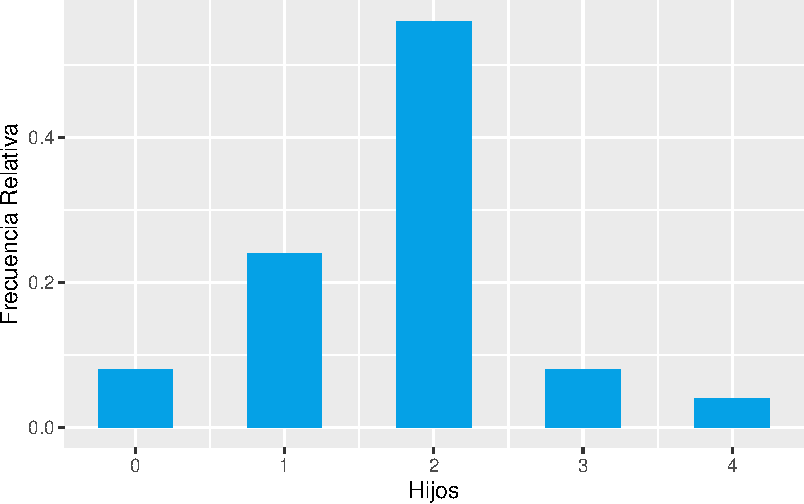
\includegraphics{02-estadistica-descriptiva_files/figure-pdf/diagrama-barras-relativas-1.pdf}

El diagrama de barras que aparece a continuación muestra la distribución
de frecuencias absolutas acumuladas del número de hijos en la muestra
anterior.

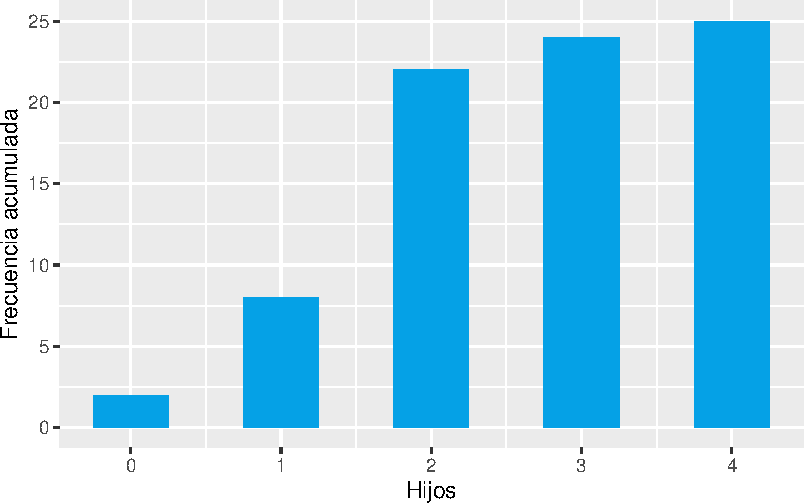
\includegraphics{02-estadistica-descriptiva_files/figure-pdf/diagrama-barras-acumuladas-1.pdf}

Y el diagrama de barras que aparece a continuación muestra la
distribución de frecuencias relativas acumuladas del número de hijos en
la muestra anterior.

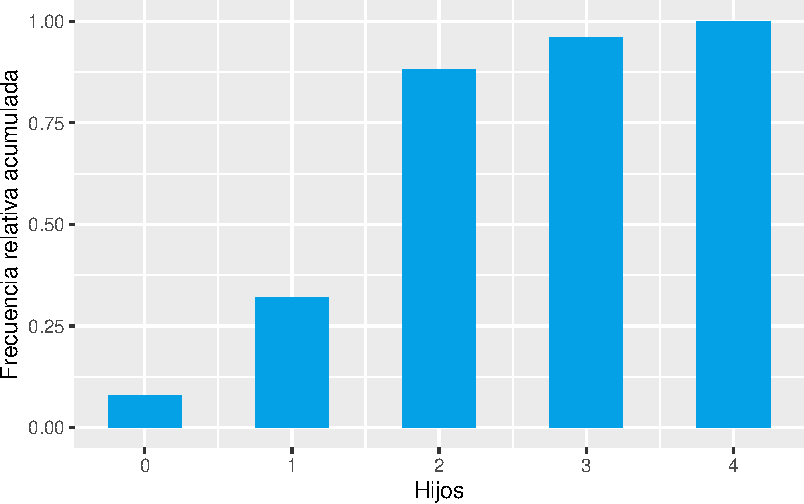
\includegraphics{02-estadistica-descriptiva_files/figure-pdf/diagrama-barras-relativas-acumuladas-1.pdf}

Finalmente, el último diagrama muestra el polígono de frecuencias
relativas acumuladas.

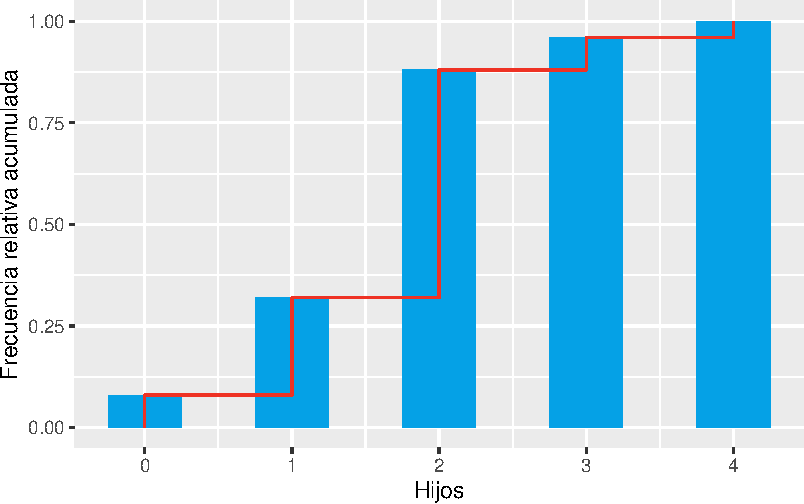
\includegraphics{02-estadistica-descriptiva_files/figure-pdf/poligono-relativas-acumuladas-1.pdf}

\end{example}

\subsection{Histograma}\label{histograma}

Un \emph{histograma} es similar a un diagrama de barras pero para datos
agrupados.

Habitualmente las clases o intervalos de agrupación se representan en el
eje \(X\), y las frecuencias en el eje \(Y\). Para cada clase se dibuja
una barra de altura la correspondiente frecuencia. A diferencia del
diagrama de barras, la anchura del la barra coincide con la anchura de
las clases y no hay separación entre dos barras consecutivas.

Dependiendo del tipo de frecuencia representada en el eje \(Y\) existen
distintos tipos de histogramas.

Al igual que con el diagrama de barras, se puede dibujar un
\emph{polígono de frecuencias} uniendo los puntos centrales más altos de
cada barra con segmentos.

\begin{example}[]\protect\hypertarget{exm-histograma}{}\label{exm-histograma}

El siguiente histograma muestra la distribución de frecuencias absolutas
de las estaturas.

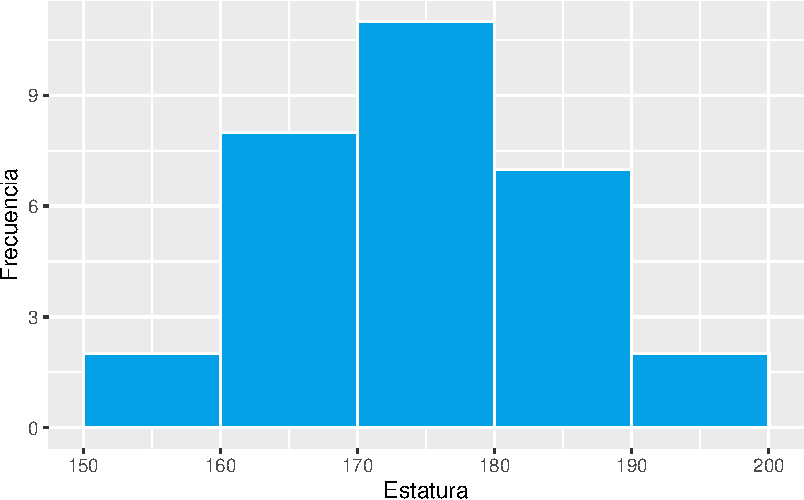
\includegraphics{02-estadistica-descriptiva_files/figure-pdf/histograma-1.pdf}

El siguiente histograma muestra la distribución de frecuencias relativas
con el polígono de frecuencias.

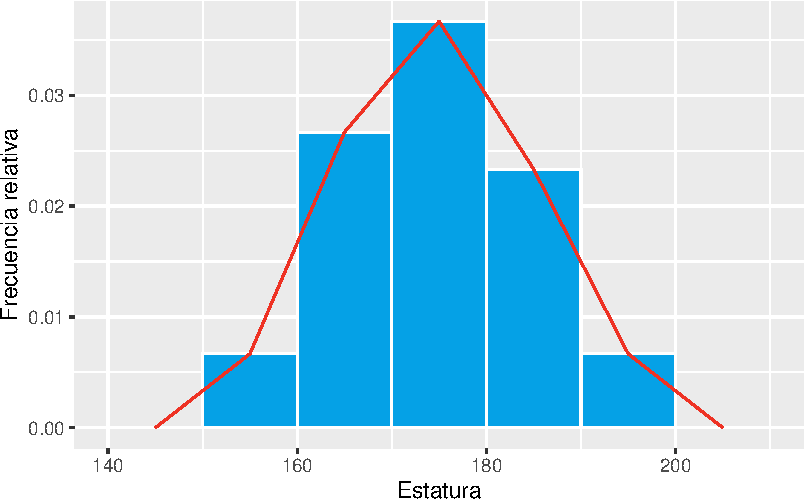
\includegraphics{02-estadistica-descriptiva_files/figure-pdf/histograma-frecuencias-relativas-1.pdf}

\end{example}

El polígono de frecuencias acumuladas (absolutas o relativas) se conoce
como \textbf{ojiva}.

\begin{example}[]\protect\hypertarget{exm-ojiva}{}\label{exm-ojiva}

El histograma y la ojiva siguientes muestran la distribución de
frecuencias relativas acumuladas de estaturas.

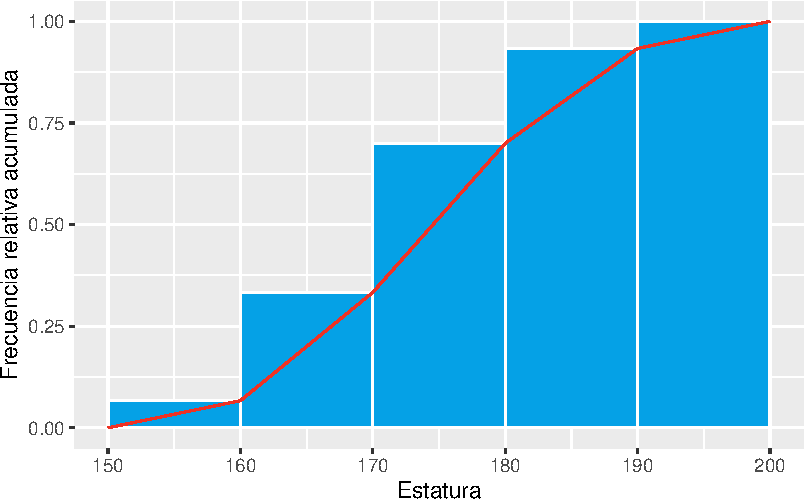
\includegraphics{02-estadistica-descriptiva_files/figure-pdf/histograma-frecuencias-relativas-acumuladas-1.pdf}

\end{example}

Obsérvese que en la ojiva se unen los vértices superiores derechos de
cada barra con segmentos, en lugar de los puntos centrales, ya que no se
consigue alcanzar la frecuencia acumulada correspondiente a la clase
hasta que no se alcanza el final del intervalo.

\subsection{Diagrama de sectores}\label{diagrama-de-sectores}

Un \emph{diagrama de sectores} consiste en un círculo divido en
porciones, uno por cada valor o categoría de la variable. Cada porción
se conoce como \emph{sector} y su ángulo o área es proporcional a la
correspondiente frecuencia del valor o categoría.

Los diagramas de sectores pueden representar frecuencias absolutas o
relativas, pero no pueden representar frecuencias acumuladas, y se
utilizan sobre todo con atributos nominales. Para atributos ordinales o
variables cuantitativas es mejor utilizar diagramas de barras, ya es más
fácil percibir las diferencias en una dimensión (altura de las barras)
que en dos dimensiones (áreas de los sectores).

\begin{example}[]\protect\hypertarget{exm-diagrama-sectores}{}\label{exm-diagrama-sectores}

El diagrama de sectores siguiente muestra la distribución de frecuencias
relativas de los grupos sanguíneos.

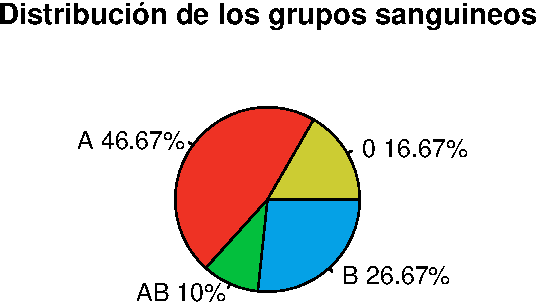
\includegraphics{02-estadistica-descriptiva_files/figure-pdf/diagrama-sectores-1.pdf}

\end{example}

\subsection{La distribución Normal}\label{la-distribuciuxf3n-normal}

Las distribuciones con diferentes propiedades presentan formas
distintas.

\begin{example}[Distribución de los ingresos
familiares]\protect\hypertarget{exm-distribucion-ingresos-familiares}{}\label{exm-distribucion-ingresos-familiares}

~

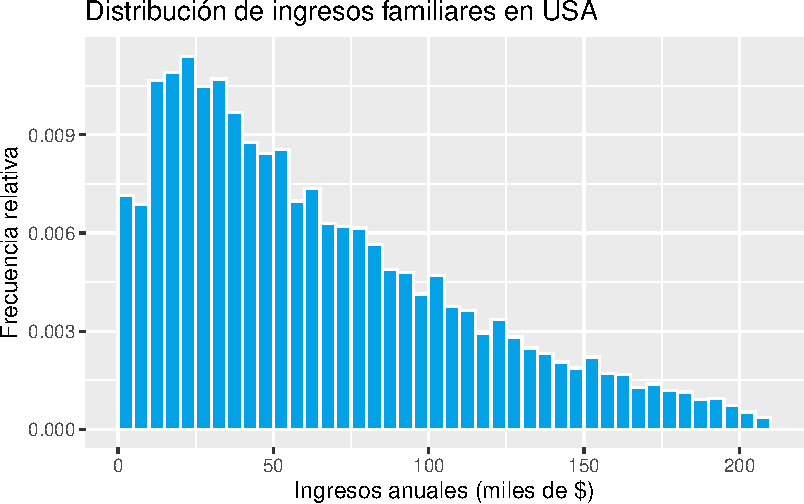
\includegraphics{02-estadistica-descriptiva_files/figure-pdf/histograma-ingresos-familiares-1.pdf}

\end{example}

\begin{example}[Distribución de la edad de
fallecimiento]\protect\hypertarget{exm-distribucion-edad-fallecimiento}{}\label{exm-distribucion-edad-fallecimiento}

~

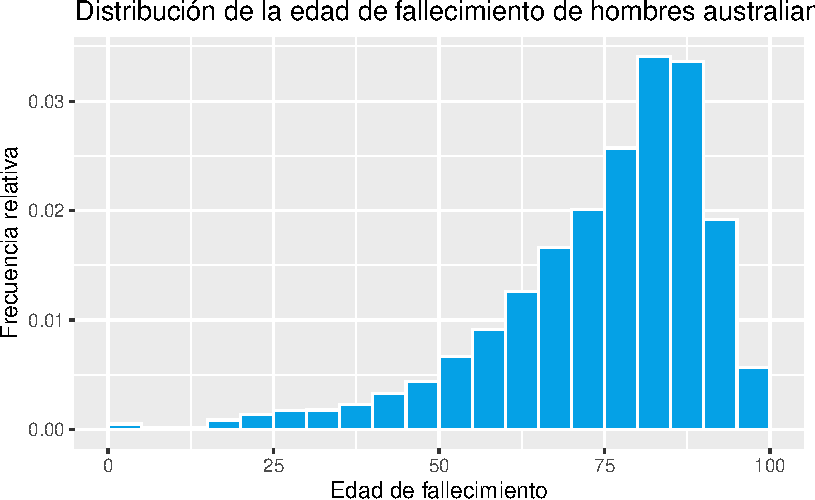
\includegraphics{02-estadistica-descriptiva_files/figure-pdf/histograma-edad-fallecimiento-1.pdf}

\end{example}

\begin{example}[Distribución del tiempo de espera del
metro]\protect\hypertarget{exm-distribucion-tiempo-espera-metro}{}\label{exm-distribucion-tiempo-espera-metro}

~

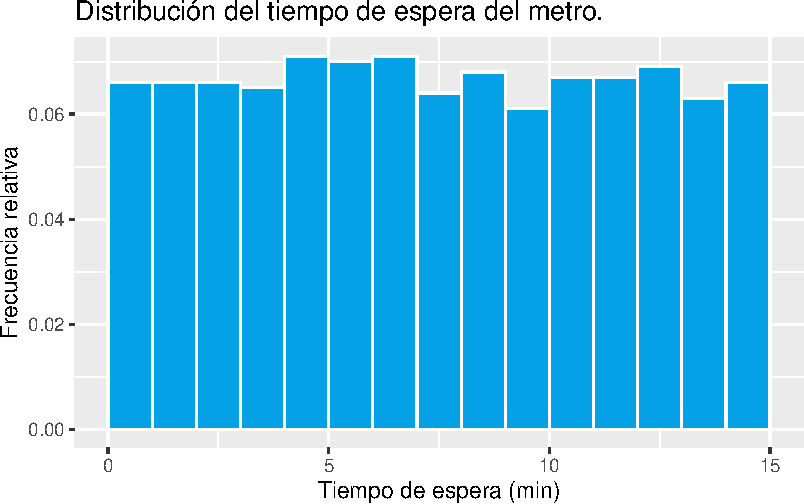
\includegraphics{02-estadistica-descriptiva_files/figure-pdf/histograma-tiempo-espera-metro-1.pdf}

\end{example}

\begin{example}[Distribución del tiempo de llegada de clientes a un
restaurante]\protect\hypertarget{exm-distribucion-llegada-clientes-restaurantes}{}\label{exm-distribucion-llegada-clientes-restaurantes}

~

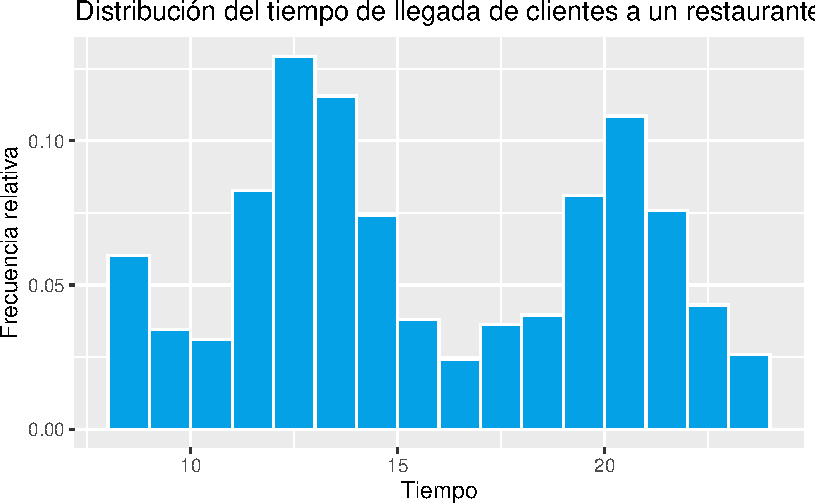
\includegraphics{02-estadistica-descriptiva_files/figure-pdf/histograma-tiempo-llegada-restaurante-1.pdf}

\end{example}

Las distribuciones con forma de campana se presentan muy a menudo en las
variables biológicas.

\begin{example}[Distribución del peso de los
hombres]\protect\hypertarget{exm-distribucion-peso-hombres}{}\label{exm-distribucion-peso-hombres}

~

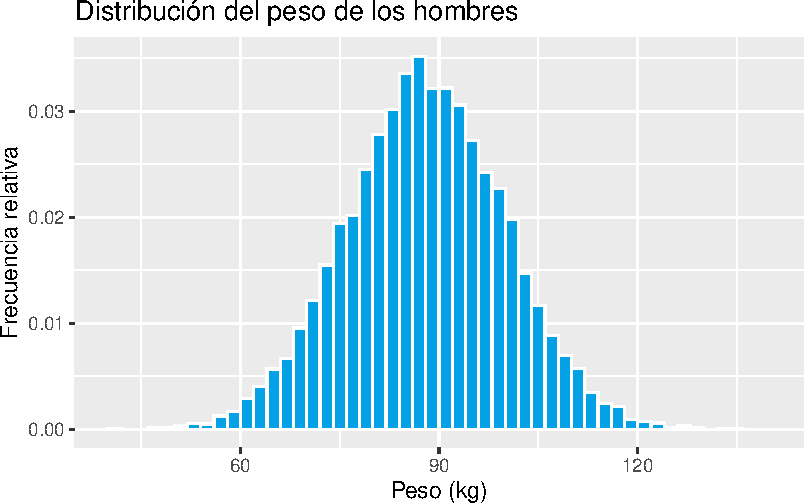
\includegraphics{02-estadistica-descriptiva_files/figure-pdf/histograma-peso-hombres-1.pdf}

\end{example}

\begin{example}[Distribución de la estatura de las
mujeres]\protect\hypertarget{exm-distribucion-estatura-mujeres}{}\label{exm-distribucion-estatura-mujeres}

~

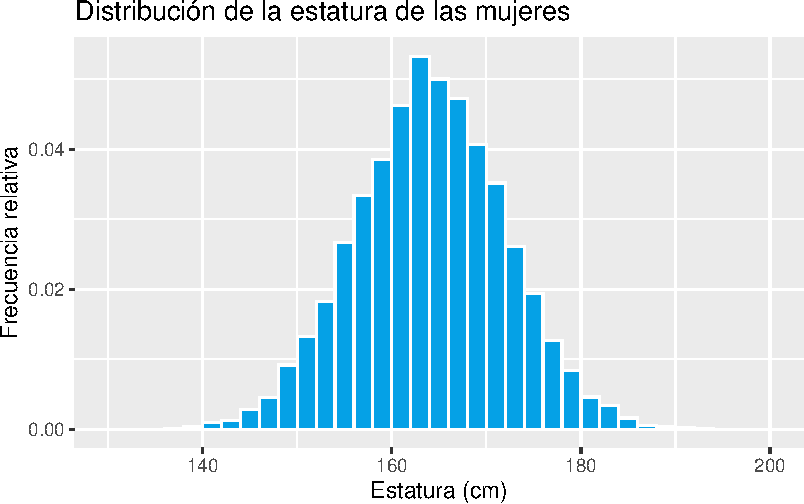
\includegraphics{02-estadistica-descriptiva_files/figure-pdf/histograma-estatura-mujeres-1.pdf}

\end{example}

\begin{example}[Distribución de la estatura según el
sexo]\protect\hypertarget{exm-distribucion-estaturas-sexo}{}\label{exm-distribucion-estaturas-sexo}

~

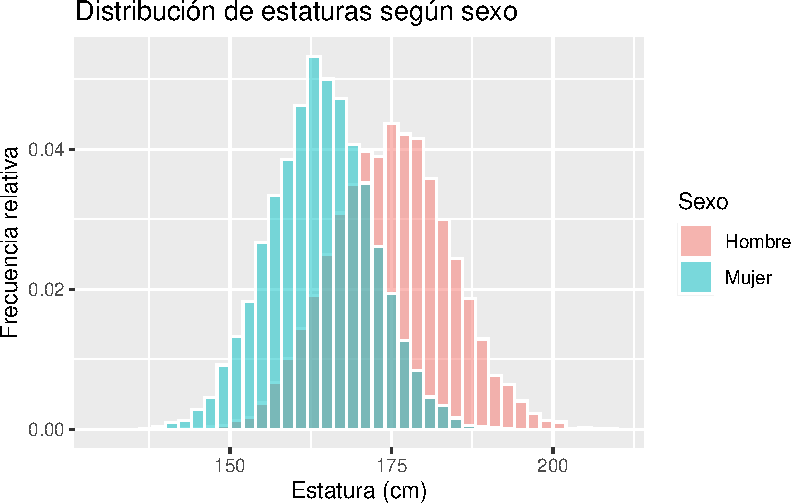
\includegraphics{02-estadistica-descriptiva_files/figure-pdf/histograma-estatura-sexo-1.pdf}

\end{example}

\begin{example}[Distribución de la estatura de hombres y
mujeres]\protect\hypertarget{exm-distribucion-estaturas-ambos-sexos}{}\label{exm-distribucion-estaturas-ambos-sexos}

~

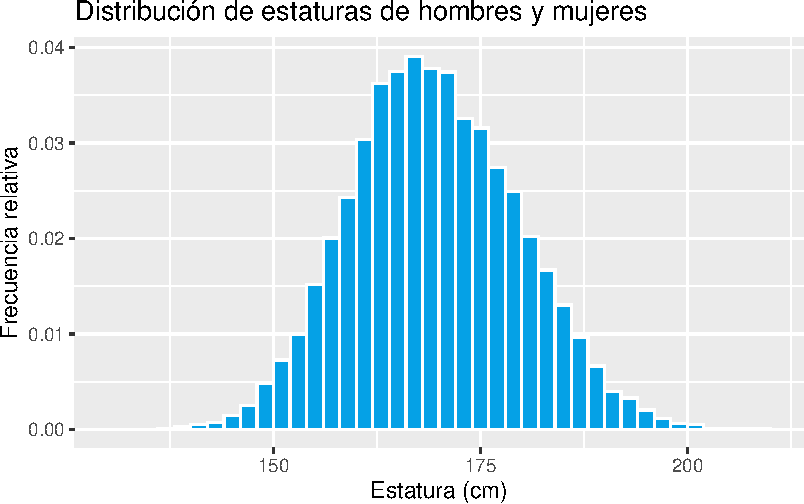
\includegraphics{02-estadistica-descriptiva_files/figure-pdf/histograma-estatura-ambos-sexo-1.pdf}

\end{example}

\begin{example}[Distribución del
colesterol]\protect\hypertarget{exm-distribucion-colesterol}{}\label{exm-distribucion-colesterol}

~

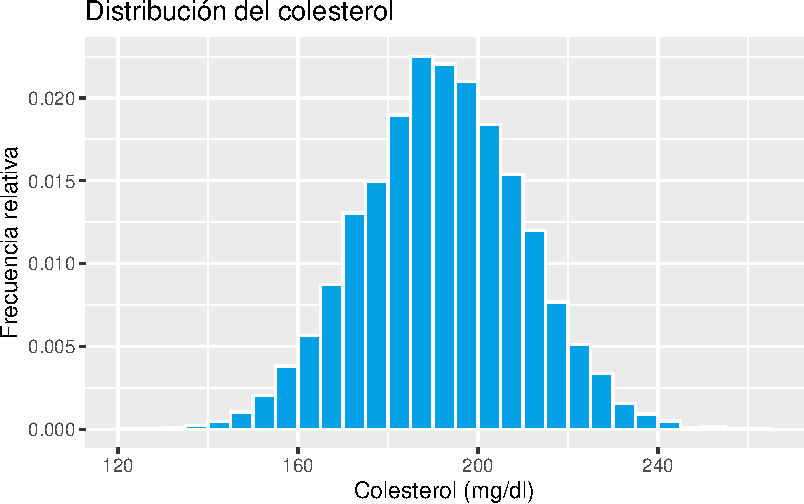
\includegraphics{02-estadistica-descriptiva_files/figure-pdf/histograma-colesterol-1.pdf}

\end{example}

\begin{example}[Distribución de
notas]\protect\hypertarget{exm-distribucion-notas}{}\label{exm-distribucion-notas}

~

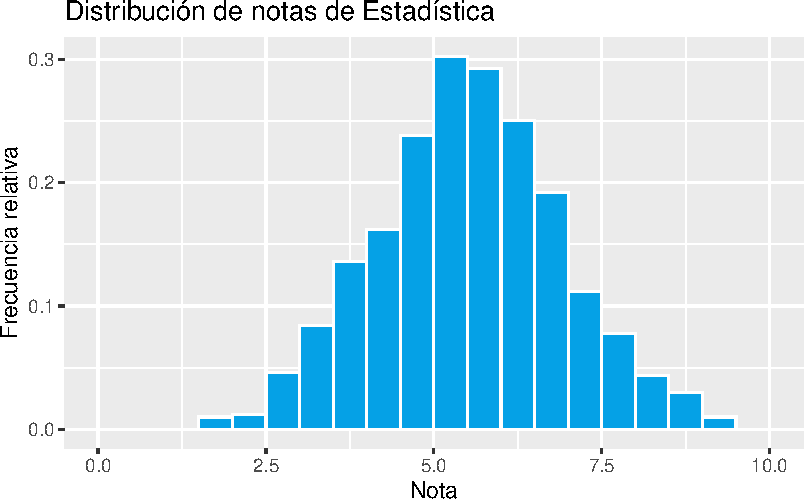
\includegraphics{02-estadistica-descriptiva_files/figure-pdf/histograma-notas-1.pdf}

\end{example}

La distribución con forma de campana aparece tan a menudo en la
Naturaleza que se conoce como \emph{distribución normal} o
\emph{distribución gaussiana}.

\begin{figure}
\centering
% Created by tikzDevice version 0.12.3 on 2019-09-02 00:52:27
% !TEX encoding = UTF-8 Unicode
\begin{tikzpicture}[x=1pt,y=1pt]
\definecolor{fillColor}{RGB}{255,255,255}
\path[use as bounding box,fill=fillColor,fill opacity=0.00] (0,0) rectangle (505.89,361.35);
\begin{scope}
\path[clip] ( 49.20, 61.20) rectangle (480.69,312.15);
\definecolor{drawColor}{RGB}{238,50,36}

\path[draw=drawColor,line width= 1.2pt,line join=round,line cap=round] ( 65.18, 71.38) --
	( 68.21, 71.54) --
	( 71.23, 71.73) --
	( 74.26, 71.94) --
	( 77.29, 72.18) --
	( 80.31, 72.46) --
	( 83.34, 72.78) --
	( 86.37, 73.15) --
	( 89.39, 73.57) --
	( 92.42, 74.04) --
	( 95.45, 74.58) --
	( 98.48, 75.19) --
	(101.50, 75.88) --
	(104.53, 76.65) --
	(107.56, 77.51) --
	(110.58, 78.47) --
	(113.61, 79.55) --
	(116.64, 80.74) --
	(119.66, 82.06) --
	(122.69, 83.52) --
	(125.72, 85.12) --
	(128.74, 86.88) --
	(131.77, 88.81) --
	(134.80, 90.92) --
	(137.82, 93.21) --
	(140.85, 95.69) --
	(143.88, 98.37) --
	(146.90,101.27) --
	(149.93,104.38) --
	(152.96,107.71) --
	(155.98,111.26) --
	(159.01,115.04) --
	(162.04,119.06) --
	(165.06,123.30) --
	(168.09,127.77) --
	(171.12,132.46) --
	(174.14,137.37) --
	(177.17,142.49) --
	(180.20,147.81) --
	(183.22,153.31) --
	(186.25,158.98) --
	(189.28,164.81) --
	(192.30,170.76) --
	(195.33,176.83) --
	(198.36,182.98) --
	(201.38,189.20) --
	(204.41,195.44) --
	(207.44,201.68) --
	(210.46,207.89) --
	(213.49,214.03) --
	(216.52,220.08) --
	(219.54,225.99) --
	(222.57,231.73) --
	(225.60,237.26) --
	(228.62,242.56) --
	(231.65,247.58) --
	(234.68,252.29) --
	(237.70,256.66) --
	(240.73,260.65) --
	(243.76,264.25) --
	(246.78,267.43) --
	(249.81,270.15) --
	(252.84,272.41) --
	(255.86,274.19) --
	(258.89,275.46) --
	(261.92,276.23) --
	(264.94,276.49) --
	(267.97,276.23) --
	(271.00,275.46) --
	(274.03,274.19) --
	(277.05,272.41) --
	(280.08,270.15) --
	(283.11,267.43) --
	(286.13,264.25) --
	(289.16,260.65) --
	(292.19,256.66) --
	(295.21,252.29) --
	(298.24,247.58) --
	(301.27,242.56) --
	(304.29,237.26) --
	(307.32,231.73) --
	(310.35,225.99) --
	(313.37,220.08) --
	(316.40,214.03) --
	(319.43,207.89) --
	(322.45,201.68) --
	(325.48,195.44) --
	(328.51,189.20) --
	(331.53,182.98) --
	(334.56,176.83) --
	(337.59,170.76) --
	(340.61,164.81) --
	(343.64,158.98) --
	(346.67,153.31) --
	(349.69,147.81) --
	(352.72,142.49) --
	(355.75,137.37) --
	(358.77,132.46) --
	(361.80,127.77) --
	(364.83,123.30) --
	(367.85,119.06) --
	(370.88,115.04) --
	(373.91,111.26) --
	(376.93,107.71) --
	(379.96,104.38) --
	(382.99,101.27) --
	(386.01, 98.37) --
	(389.04, 95.69) --
	(392.07, 93.21) --
	(395.09, 90.92) --
	(398.12, 88.81) --
	(401.15, 86.88) --
	(404.17, 85.12) --
	(407.20, 83.52) --
	(410.23, 82.06) --
	(413.25, 80.74) --
	(416.28, 79.55) --
	(419.31, 78.47) --
	(422.33, 77.51) --
	(425.36, 76.65) --
	(428.39, 75.88) --
	(431.41, 75.19) --
	(434.44, 74.58) --
	(437.47, 74.04) --
	(440.50, 73.57) --
	(443.52, 73.15) --
	(446.55, 72.78) --
	(449.58, 72.46) --
	(452.60, 72.18) --
	(455.63, 71.94) --
	(458.66, 71.73) --
	(461.68, 71.54) --
	(464.71, 71.38);
\end{scope}
\begin{scope}
\path[clip] (  0.00,  0.00) rectangle (505.89,361.35);
\definecolor{drawColor}{RGB}{0,0,0}

\node[text=drawColor,anchor=base,inner sep=0pt, outer sep=0pt, scale=  1.20] at (264.94,332.61) {\bfseries Gauss bell};
\end{scope}
\end{tikzpicture}

\caption{Campana de Gauss.}
\end{figure}

\section{Datos atípicos}\label{datos-atuxedpicos}

Uno de los principales problemas de las muestras son los \textbf{datos
atípicos}, que son valores de la variable que se diferencian mucho del
resto de los valores en la muestra.

\begin{figure}[H]

{\centering 
\includegraphics{img/descriptiva/dato_atipico.png}

}

\caption{Dato atípico.}

\end{figure}%

Es muy importante detectar los datos atípicos antes de realizar
cualquier análisis de los datos, pues suelen distorsionar los
resultados.

Aparecen siempre en los extremos de la distribución, y pueden detectarse
con un diagrama de caja y bigotes (tal y como veremos más adelante).

\subsection{Tratamiento de los datos
atípicos}\label{tratamiento-de-los-datos-atuxedpicos}

Cuando trabajemos con muestras grandes, los datos atípicos tienen menor
influencia y pueden dejarse en la muestra.

Cuando trabajemos con muestras pequeñas tenemos varias opciones:

\begin{itemize}
\tightlist
\item
  Eliminar el dato atípico si se trata de un error.
\item
  Sustituir el dato atípico por el menor o el mayor valor de la
  distribución que no es atípico si no se trata de un error y el dato
  atípico no concuerda con la distribución teórica.
\item
  Dejar el dato atípico si no es un error, y cambiar el modelo de
  distribución teórico para adecuarlo a los datos atípicos.
\end{itemize}

\section{Estadísticos muestrales}\label{estaduxedsticos-muestrales}

La tabla de frecuencias sintetiza la información de la distribución de
valores de la variable estudiada en la muestra, pero en muchas ocasiones
es insuficiente para describir determinados aspectos de la distribución,
como por ejemplo, cuáles son los valores más representativos de la
muestra, cómo es la variabilidad de los datos, qué datos pueden
considerarse atípicos, o cómo es la simetría de la distribución.

Para describir esos aspectos de la distribución muestral se utilizan
unas medidas resumen llamadas \textbf{estadísticos muestrales}.

De acuerdo al aspecto de las distribución que miden, existen diferentes
tipos de estadísticos:

\textbf{Estadísticos de Posición}: Miden los valores en torno a los que
se agrupan los datos o que dividen la distribución en partes iguales.

\textbf{Estadísticos de Dispersión}: Miden la heterogeneidad de los
datos.

\textbf{Estadísticos de Forma}: Miden aspectos de la forma que tiene la
distribución de los datos, como la simetría o el apuntamiento.

\section{Estadísticos de posición}\label{estaduxedsticos-de-posiciuxf3n}

Pueden ser de dos tipos:

\textbf{Estadísticos de Tendencia Central}: Determinan valores alrededor
de los cuales se concentran los datos, habitualmente en el centro de la
distribución. Estas medidas suelen utilizarse como valores
representativos de la muestra. Las más importantes son:

\begin{itemize}
\tightlist
\item
  Media aritmética
\item
  Mediana
\item
  Moda
\end{itemize}

\textbf{Estadísticos de Posición no centrales}: Dividen la distribución
en partes con el mismo número de datos. Las más importantes son:

\begin{itemize}
\tightlist
\item
  Cuartiles.
\item
  Deciles.
\item
  Percentiles.
\end{itemize}

\subsection{Media aritmética}\label{media-aritmuxe9tica}

\begin{definition}[Media aritmética muestral
\(\bar{x}\)]\protect\hypertarget{def-media-aritmetica}{}\label{def-media-aritmetica}

La \emph{media aritmética muestral} de una variable \(X\) es la suma de
los valores observados en la muestra dividida por el tamaño muestral

\[\bar{x} = \frac{\sum x_i}{n}\]

\end{definition}

A partir de la tabla de frecuencias puede calcularse con la fórmula

\[\bar{x} = \frac{\sum x_in_i}{n} = \sum x_i f_i\]

En la mayoría de los casos, la media aritmética es la medida que mejor
representa a la muestra.

\begin{tcolorbox}[enhanced jigsaw, title=\textcolor{quarto-callout-warning-color}{\faExclamationTriangle}\hspace{0.5em}{Advertencia}, coltitle=black, colframe=quarto-callout-warning-color-frame, opacitybacktitle=0.6, toprule=.15mm, breakable, opacityback=0, colbacktitle=quarto-callout-warning-color!10!white, colback=white, toptitle=1mm, rightrule=.15mm, bottomrule=.15mm, left=2mm, bottomtitle=1mm, titlerule=0mm, arc=.35mm, leftrule=.75mm]

No puede calcularse para variables cualitativas.

\end{tcolorbox}

\begin{example}[Datos no
agrupados]\protect\hypertarget{exm-media-datos-no-agrupados}{}\label{exm-media-datos-no-agrupados}

Utilizando los datos de la muestra del número de hijos en las familias,
la media aritmética es

\begin{align*}
\bar{x} &= \frac{1+2+4+2+2+2+3+2+1+1+0+2+2}{25}+\\
 &+\frac{0+2+2+1+2+2+3+1+2+2+1+2}{25} = \frac{44}{25} = 1.76 \mbox{ hijos}.
\end{align*}

o bien, desde la tabla de frecuencias

\[
\begin{array}{rrrrr}
\hline
x_i & n_i & f_i & x_in_i & x_if_i\\
\hline
0 & 2 & 0.08 & 0 & 0\\
1 & 6 & 0.24 & 6 & 0.24\\
2 & 14 & 0.56 & 28 & 1.12\\
3 & 2  & 0.08 & 6 & 0.24\\
4 & 1 & 0.04 & 4 & 0.16 \\
\hline
\sum & 25 & 1 & 44 & 1.76 \\
\hline
\end{array}
\]

\[
\bar{x} = \frac{\sum x_in_i}{n} = \frac{44}{25}= 1.76 \mbox{ hijos}\qquad \bar{x}=\sum{x_if_i} = 1.76 \mbox{ hijos}.
\]

Esto significa que el valor que mejor representa el número de hijos en
las familias de la muestra es 1.76 hijos.

\end{example}

\begin{example}[Datos
agrupados]\protect\hypertarget{exm-media-datos-agrupados}{}\label{exm-media-datos-agrupados}

Utilizando los datos de la muestra de estaturas, la media es

\[
\bar{x} = \frac{179+173+\cdots+187}{30} = 175.07 \mbox{ cm}.
\]

o bien, desde la tabla de frecuencias utilizando las marcas de clase
\(x_i\):

\[
\begin{array}{crrrrr}
\hline
X & x_i & n_i & f_i & x_in_i & x_if_i\\
\hline
(150,160] & 155 & 2 & 0.07 & 310 & 10.33\\
(160,170] & 165 & 8 & 0.27 & 1320 & 44.00\\
(170,180] & 175 & 11 & 0.36 & 1925 & 64.17\\
(180,190] & 185 & 7 & 0.23 & 1295 & 43.17\\
(190,200] & 195 & 2 & 0.07 & 390 & 13 \\
\hline
\sum &  & 30 & 1 & 5240 & 174.67 \\
\hline
\end{array}
\]

\[
\bar{x} = \frac{\sum x_in_i}{n} = \frac{5240}{30}= 174.67 \mbox{ cm} \qquad \bar{x}=\sum{x_if_i} = 174.67 \mbox{ cm}.
\]

Obsérvese que al calcular la media desde la tabla de frecuencias el
resultado difiere ligeramente del valor real obtenido directamente desde
la muestra, ya que los valores usados en los cálculos no son los datos
reales sino las marcas de clase.

\end{example}

\subsubsection{Media ponderada}\label{media-ponderada}

En algunos casos, los valores de la muestra no tienen la misma
importancia. En este caso la importancia o \emph{peso} de cada valor de
la muestra debe tenerse en cuenta al calcular la media.

\begin{definition}[Media ponderada muestral
\(\bar x_p\)]\protect\hypertarget{def-media-ponderada}{}\label{def-media-ponderada}

Dada una muestra de valores \(x_1,\ldots, x_n\) donde cada valor \(x_i\)
tiene asociado un peso \(p_i\), la \emph{media ponderada muestral} de la
variable \(X\) es la suma de los productos de cada valor observado en la
muestra por su peso, dividida por la suma de todos los pesos

\[\bar{x}_p = \frac{\sum x_ip_i}{\sum p_i}\]

\end{definition}

A partir de la tabla de frecuencias puede calcularse con la fórmula

\[\bar{x}_p = \frac{\sum x_ip_in_i}{\sum p_i}\]

\begin{example}[]\protect\hypertarget{exm-media-ponderada}{}\label{exm-media-ponderada}

Supóngase que un estudiante quiere calcular una medida que represente su
rendimiento en el curso. La nota obtenida en cada asignatura y sus
créditos son

\begin{longtable}[]{@{}ccl@{}}
\toprule\noalign{}
Asignatura & Créditos & Nota \\
\midrule\noalign{}
\endhead
\bottomrule\noalign{}
\endlastfoot
Matemáticas & 6 & 5 \\
Economía & 4 & 3 \\
Química & 8 & 6 \\
\end{longtable}

La media aritmética vale

\[\bar{x} = \frac{\sum x_i}{n} = \frac{5+3+6}{3}= 4.67 \text{ puntos}.\]

Sin embargo, esta nota no representa bien el rendimiento académico del
alumno ya que no todas las asignaturas tienen la misma importancia ni
requieren el mismo esfuerzo para aprobar. Las asignaturas con más
créditos requieren más trabajo y deben tener más peso en el cálculo de
la media.

Es más lógico usar la media ponderada como medida del rendimiento del
estudiante, tomando como pesos los créditos de cada asignatura

\[
\bar{x}_p = \frac{\sum x_ip_i}{\sum p_i} = \frac{5\cdot 6+3\cdot 4+6\cdot 8}{6+4+8}= \frac{90}{18} = 5 \text{ puntos}.
\]

\end{example}

\subsection{Mediana}\label{mediana}

\begin{definition}[Mediana muestral
\(Me\)]\protect\hypertarget{def-mediana}{}\label{def-mediana}

La \emph{mediana muestral} de una variable \(X\) es el valor de la
variable que está en el medio de la muestra ordenada.

\end{definition}

La mediana divide la distribución de la muestra en dos partes iguales,
es decir, hay el mismo número de valores por debajo y por encima de la
mediana. Por tanto, tiene frecuencias acumuladas \(N_{Me}= n/2\) y
\(F_{Me}= 0.5\).

\begin{tcolorbox}[enhanced jigsaw, title=\textcolor{quarto-callout-warning-color}{\faExclamationTriangle}\hspace{0.5em}{Advertencia}, coltitle=black, colframe=quarto-callout-warning-color-frame, opacitybacktitle=0.6, toprule=.15mm, breakable, opacityback=0, colbacktitle=quarto-callout-warning-color!10!white, colback=white, toptitle=1mm, rightrule=.15mm, bottomrule=.15mm, left=2mm, bottomtitle=1mm, titlerule=0mm, arc=.35mm, leftrule=.75mm]

No puede calcularse para variables nominales.

\end{tcolorbox}

Con datos no agrupados pueden darse varios casos:

\begin{itemize}
\tightlist
\item
  Tamaño muestral impar: La mediana es el valor que ocupa la posición
  \(\frac{n+1}{2}\).
\item
  Tamaño muestral par: La mediana es la media de los valores que ocupan
  las posiciones \(\frac{n}{2}\) y \(\frac{n}{2}+1\).
\end{itemize}

\begin{figure}[H]

{\centering 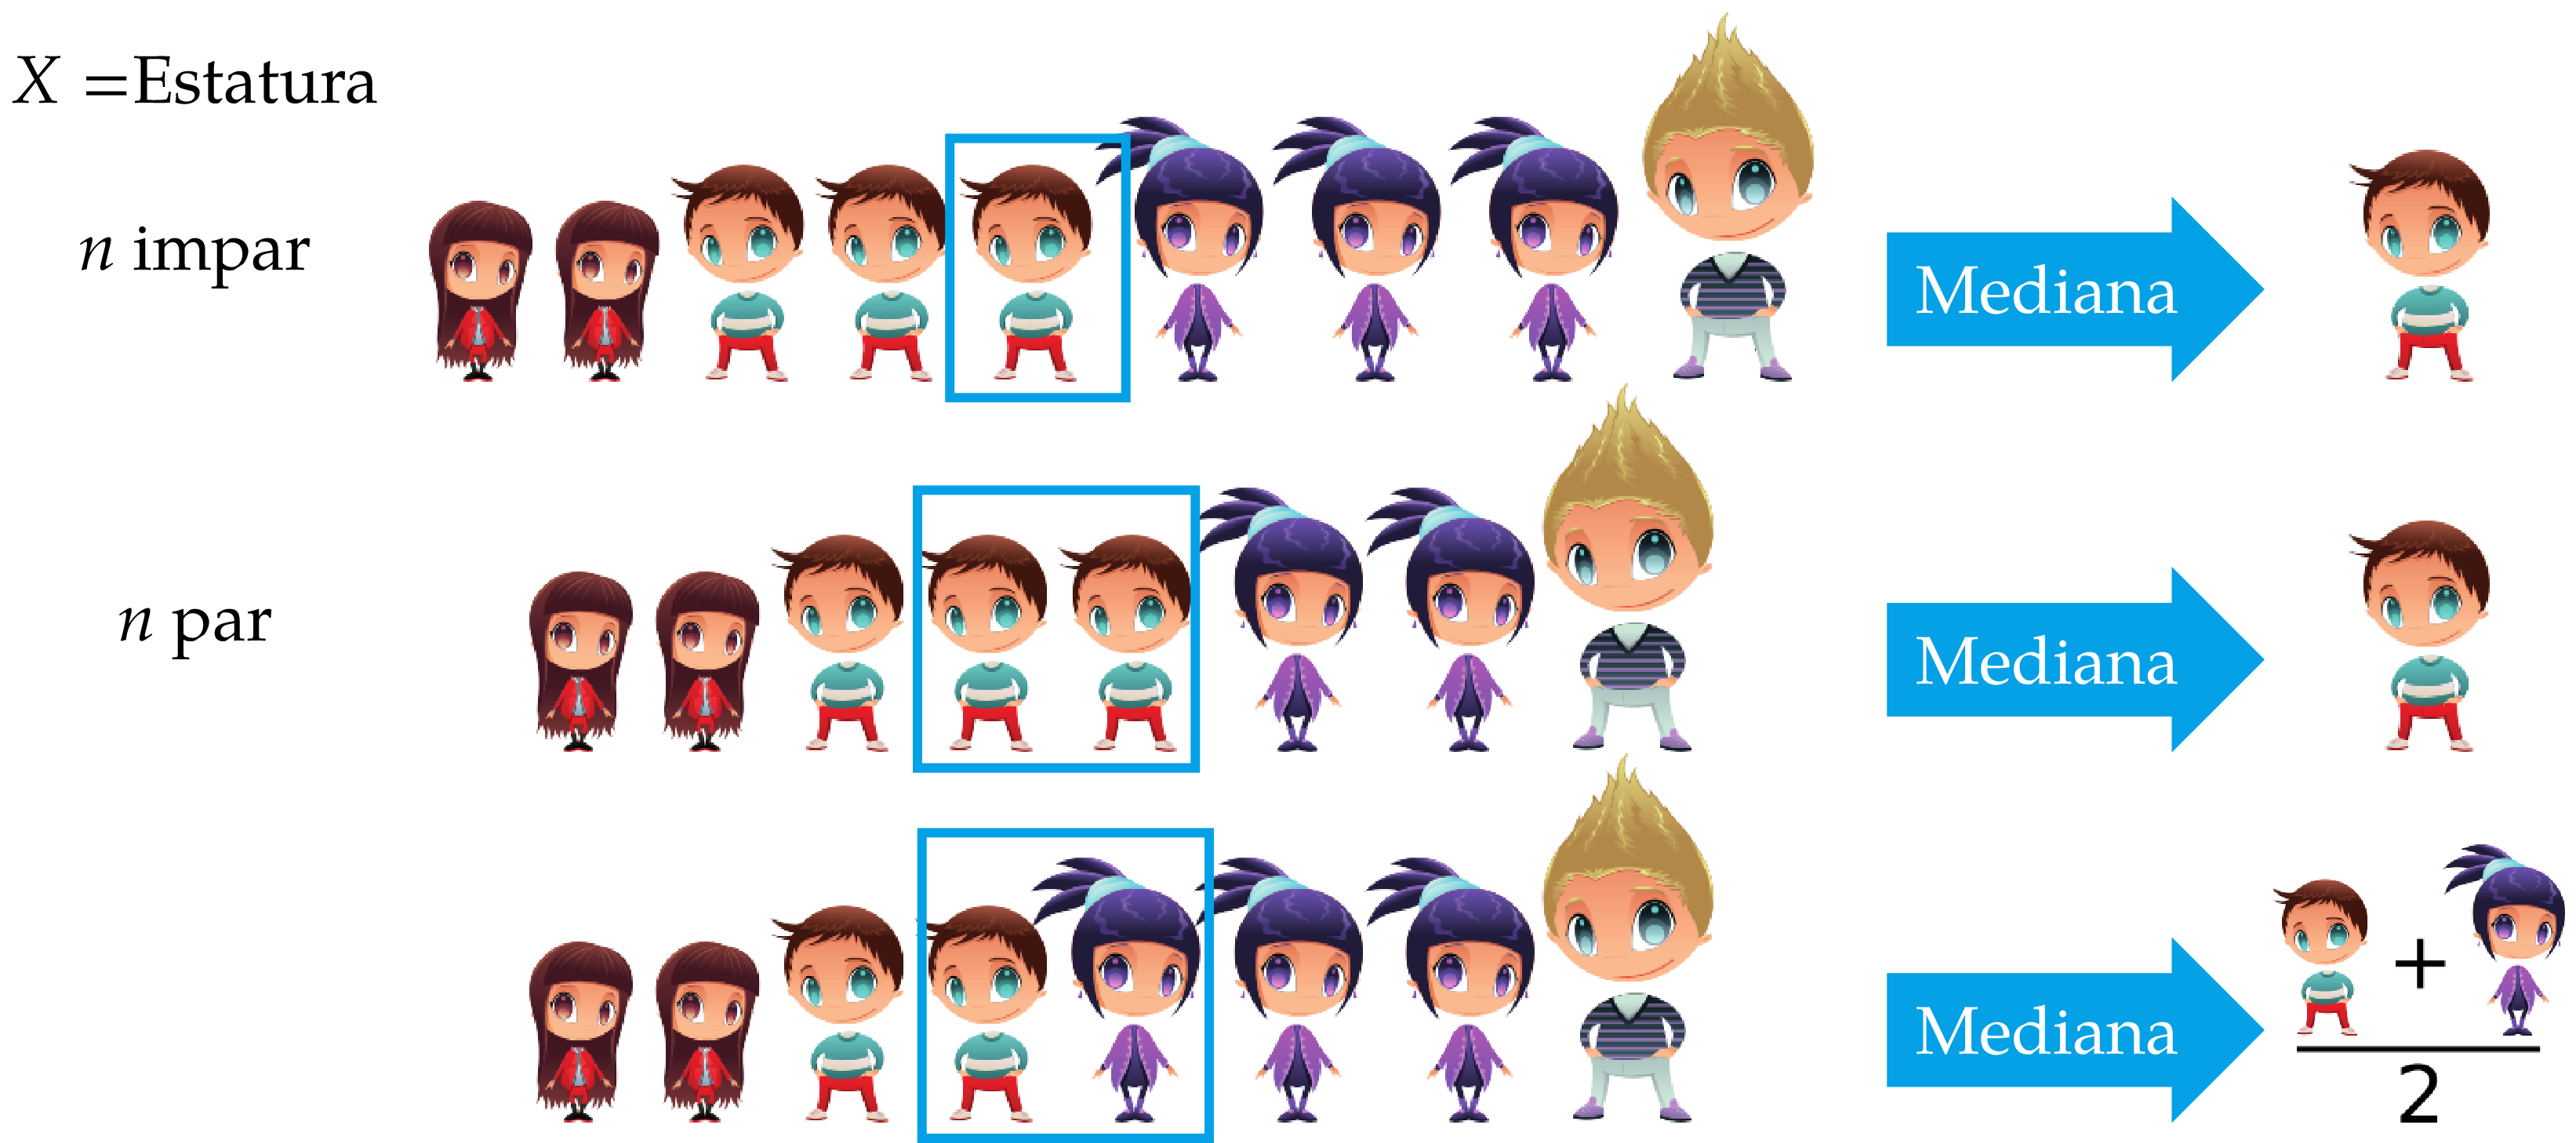
\includegraphics{img/descriptiva/mediana.png}

}

\caption{Cálculo de la mediana con datos no agrupados.}

\end{figure}%

:::\{\#exm-mediana-datos-no-agrupados\} Utilizando los datos del número
de hijos de las familias, el tamaño muestral es 25, que es impar, y la
mediana es el valor que ocupa la posición \(\frac{25+1}{2} = 13\) de la
muestra ordenada.

\[
0,0,1,1,1,1,1,1,2,2,2,2,\fbox{2},2,2,2,2,2,2,2,2,2,3,3,4
\]

y la mediana es 2 hijos.

Si se trabaja con la tabla de frecuencias, la mediana es el valor más
pequeño con una frecuencia acumulada mayor o igual a \(13\), o con una
frecuencia relativa acumulada mayor o igual que \(0.5\).

\[
\begin{array}{rrrrr}
\hline
x_i & n_i & f_i & N_i & F_i\\
\hline
0 & 2 & 0.08 & 2 & 0.08\\
1 & 6 & 0.24 & 8 & 0.32\\
\color{red}2 & 14 & 0.56 & 22 & 0.88\\
3 & 2  & 0.08 & 24 & 0.96\\
4 & 1 & 0.04 & 25 & 1 \\
\hline
\sum & 25 & 1 \\
\hline
\end{array}
\]

\subsubsection{Cálculo de la mediana con datos
agrupados}\label{cuxe1lculo-de-la-mediana-con-datos-agrupados}

Con datos agrupados la mediana se calcula interpolando en el polígono de
frecuencias relativas acumuladas para el valor 0.5.

\begin{figure}[H]

{\centering 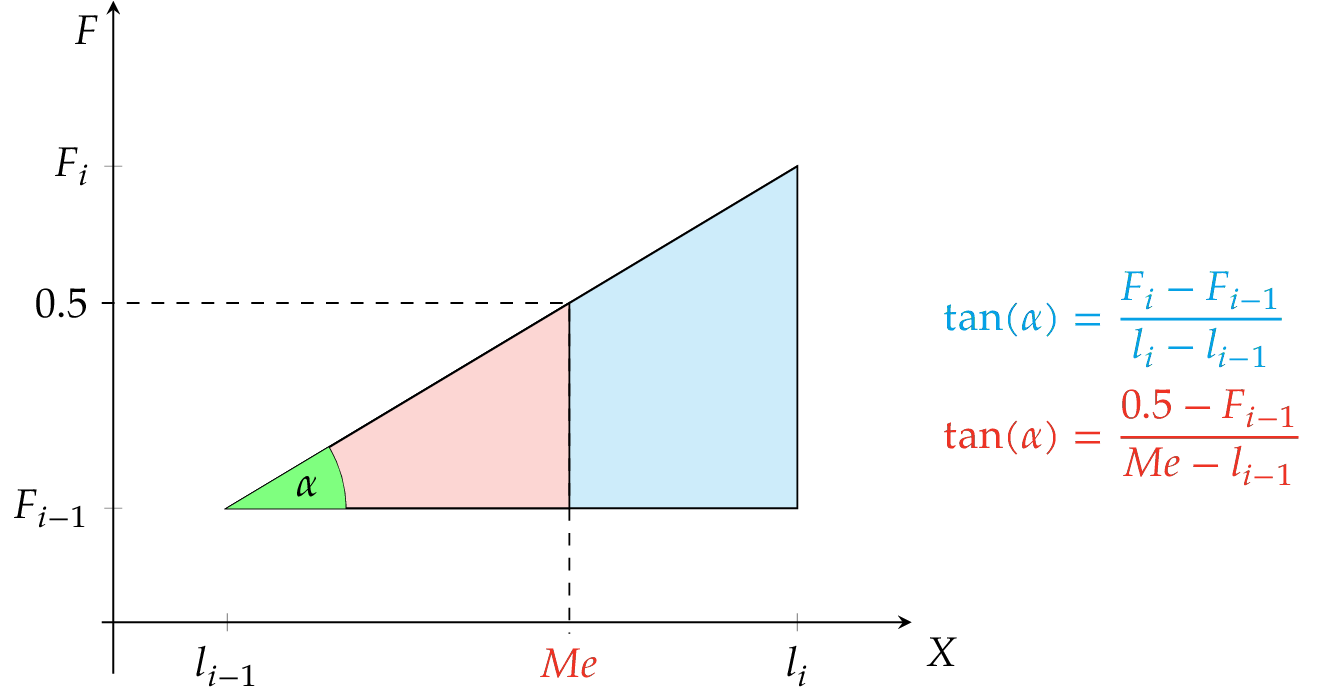
\includegraphics{img/descriptiva/interpolacion.png}

}

\caption{Cálculo de la mediana con datos agrupados.}

\end{figure}%

Ambas expresiones son iguales ya que el ángulo \(\alpha\) es el mismo, y
resolviendo la ecuación se tiene la siguiente fórmula para calcular la
mediana

\[
Me=l_i+\frac{0.5-F_{i-1}}{F_i-F_{i-1}}(l_i-l_{i-1})=l_i+\frac{0.5-F_{i-1}}{f_i}a_i
\]

\begin{example}[Datos
agrupados]\protect\hypertarget{exm-mediana-datos-agrupados}{}\label{exm-mediana-datos-agrupados}

Utilizando los datos de la muestra de las estaturas de estudiantes, la
mediana cae en la clase (170,180{]}.

\begin{figure}[H]

{\centering 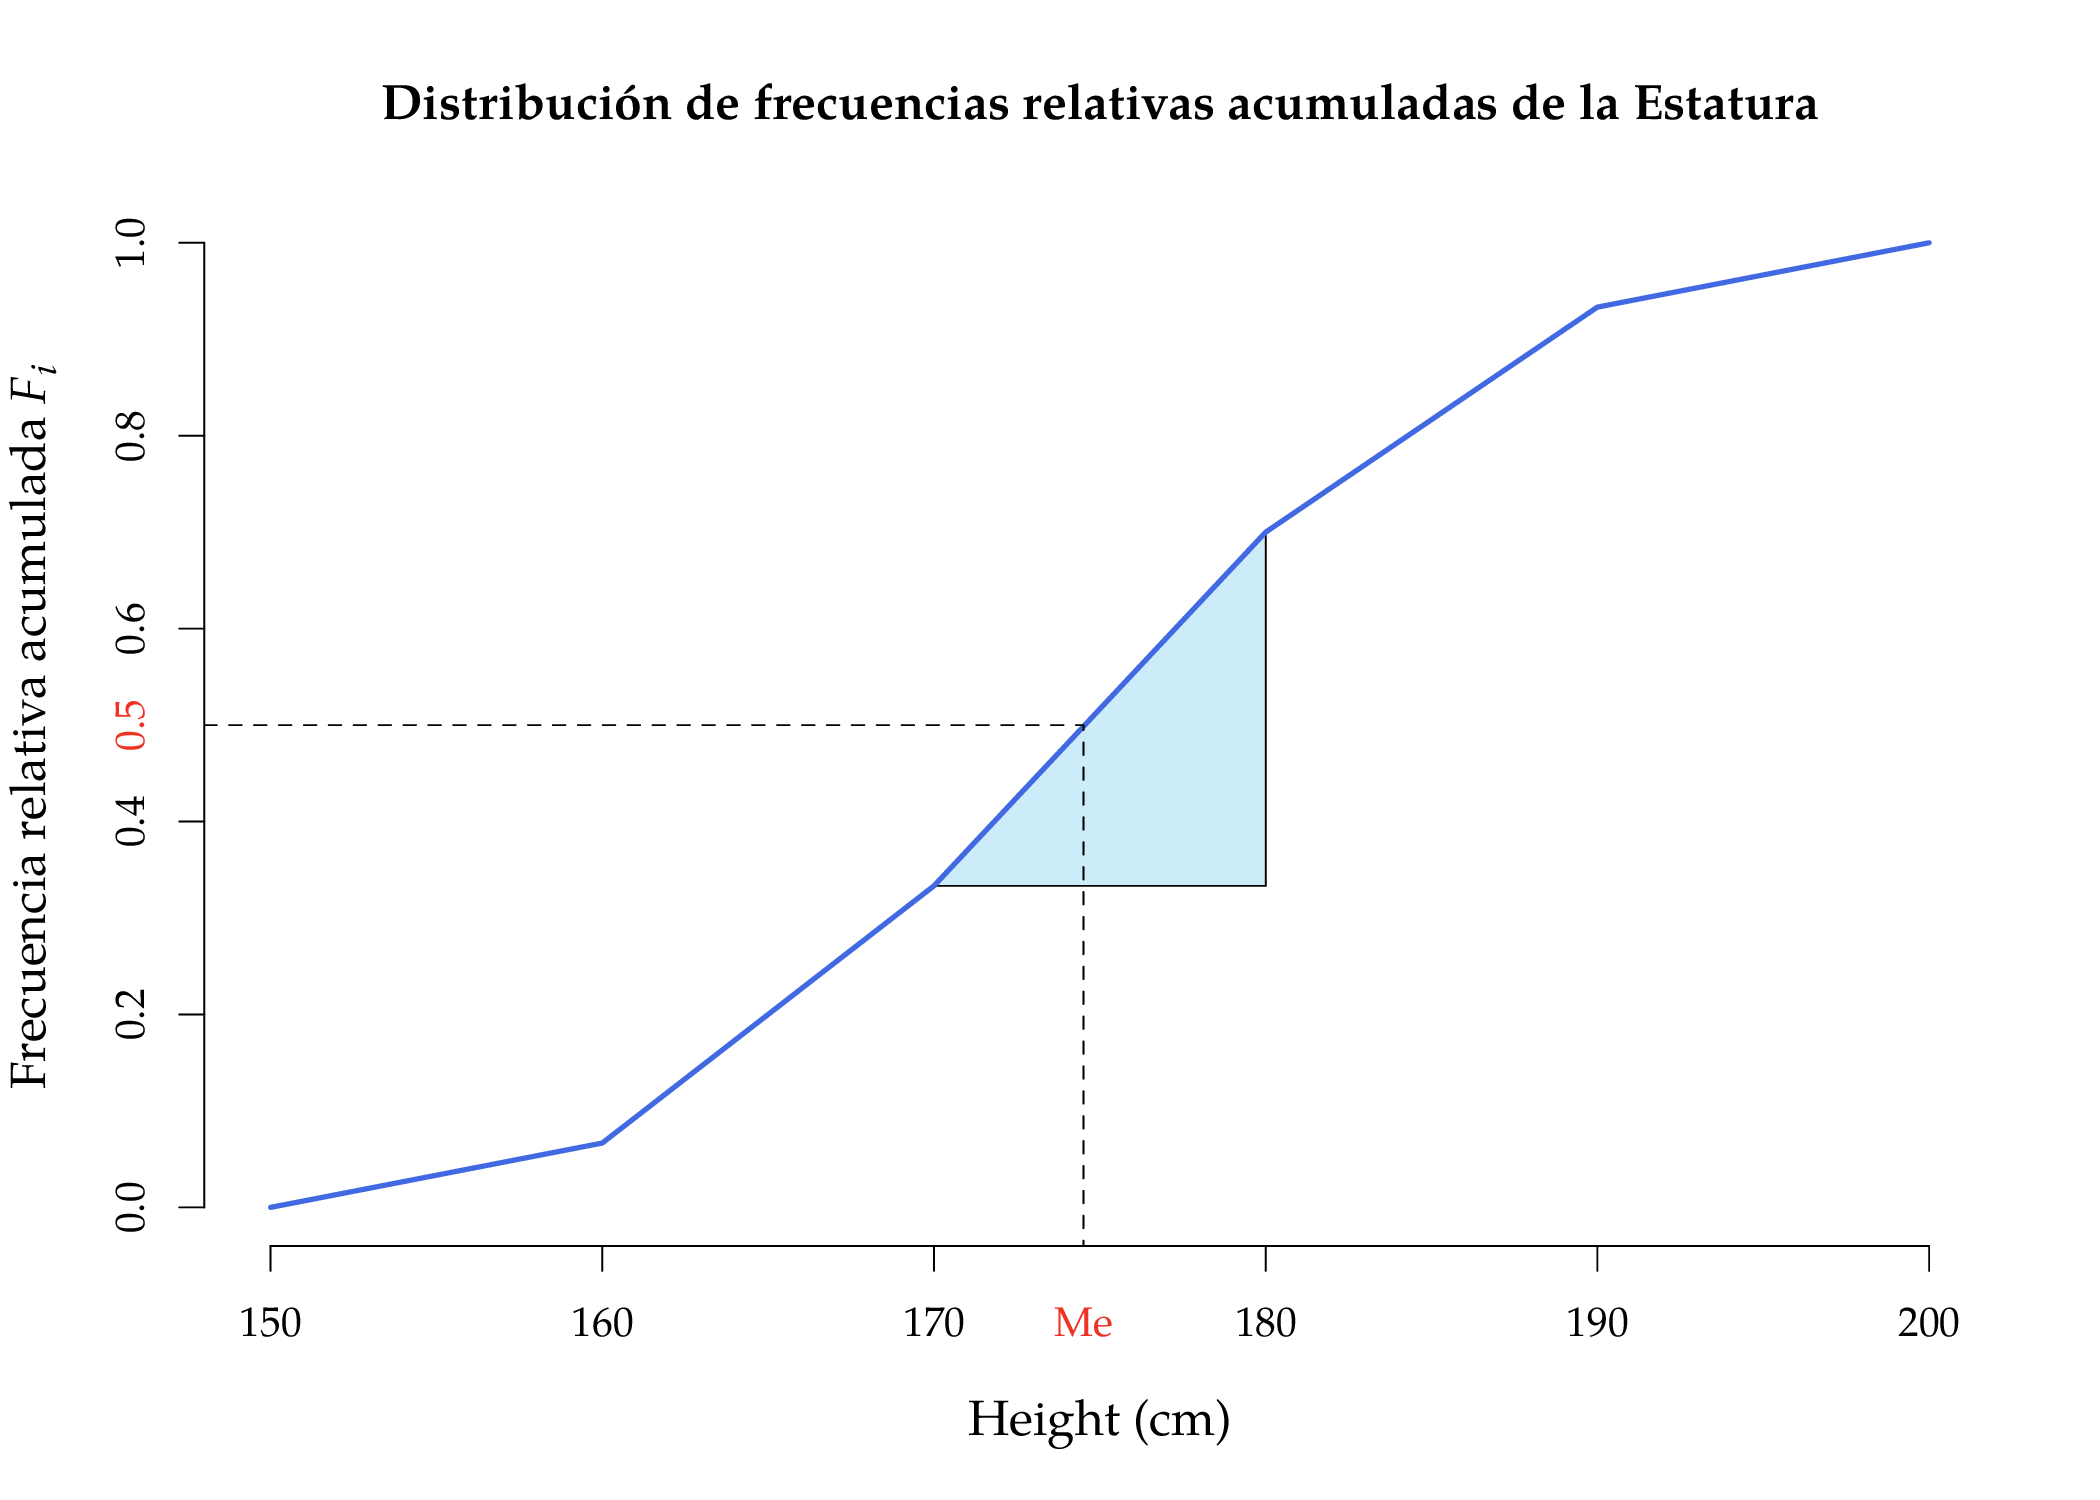
\includegraphics{img/descriptiva/interpolacion_ejemplo_1.png}

}

\caption{Ejemplo de cálculo de la mediana con datos agrupados.}

\end{figure}%

Interpolando en el intervalo (170,180{]} se tiene

\begin{figure}[H]

{\centering 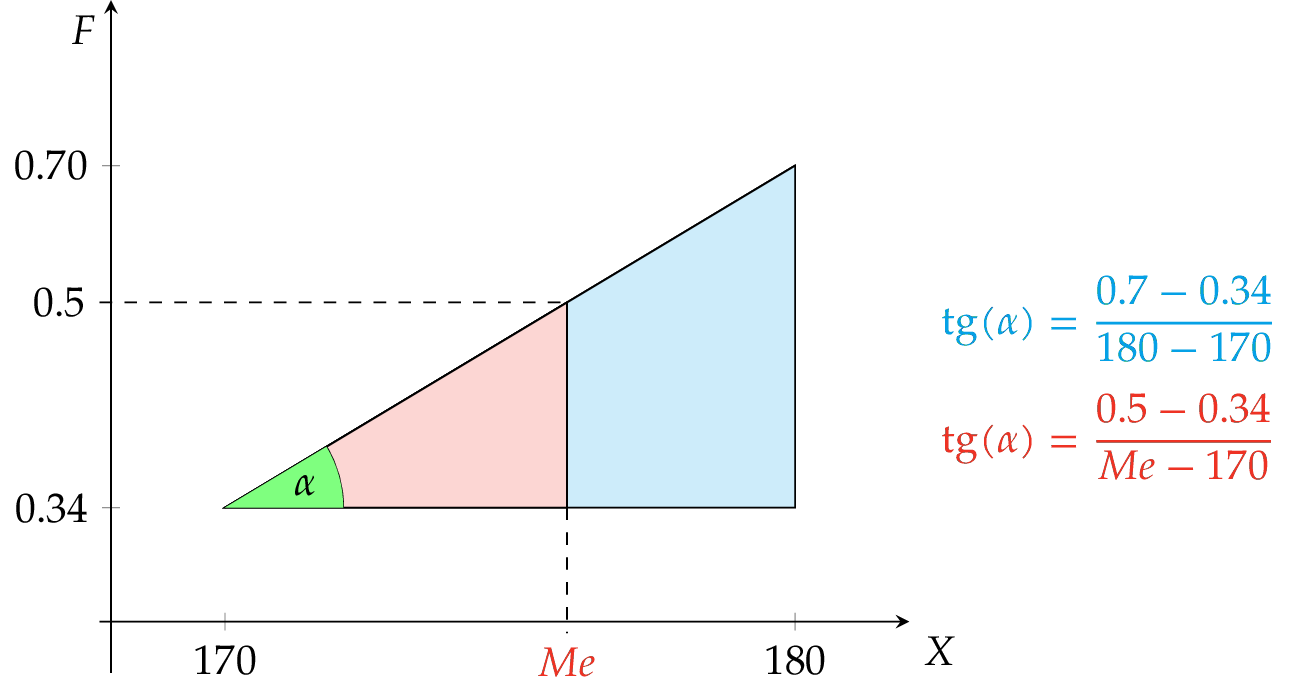
\includegraphics{img/descriptiva/interpolacion_ejemplo_2.png}

}

\caption{Ejemplo de cálculo de la mediana con datos agrupados.}

\end{figure}%

Igualando ambas expresiones y resolviendo la ecuación se obtiene

\[
Me= 170+\frac{0.5-0.34}{0.7-0.34}(180-170)=170+\frac{0.16}{0.36}10=174.54 \mbox{ cm}.
\]

Esto significa que la mitad de los estudiantes tienen estaturas menores
o iguales que 174.54 cm y la otra mitad mayores o iguales.

\end{example}

\subsection{Moda}\label{moda}

\begin{definition}[Moda muestral
\(Mo\)]\protect\hypertarget{def-moda}{}\label{def-moda}

La \emph{moda muestral} de una variable \(X\) es el valor de la variable
más frecuente en la muestra.

\end{definition}

Con datos agrupados la \emph{clase modal} es la clase con mayor
frecuencia en la muestra.

Puede calcularse para todos los tipos de variables (cuantitativas y
cualitativas).

Las distribuciones pueden tener más de una moda.

\begin{figure}[H]

{\centering 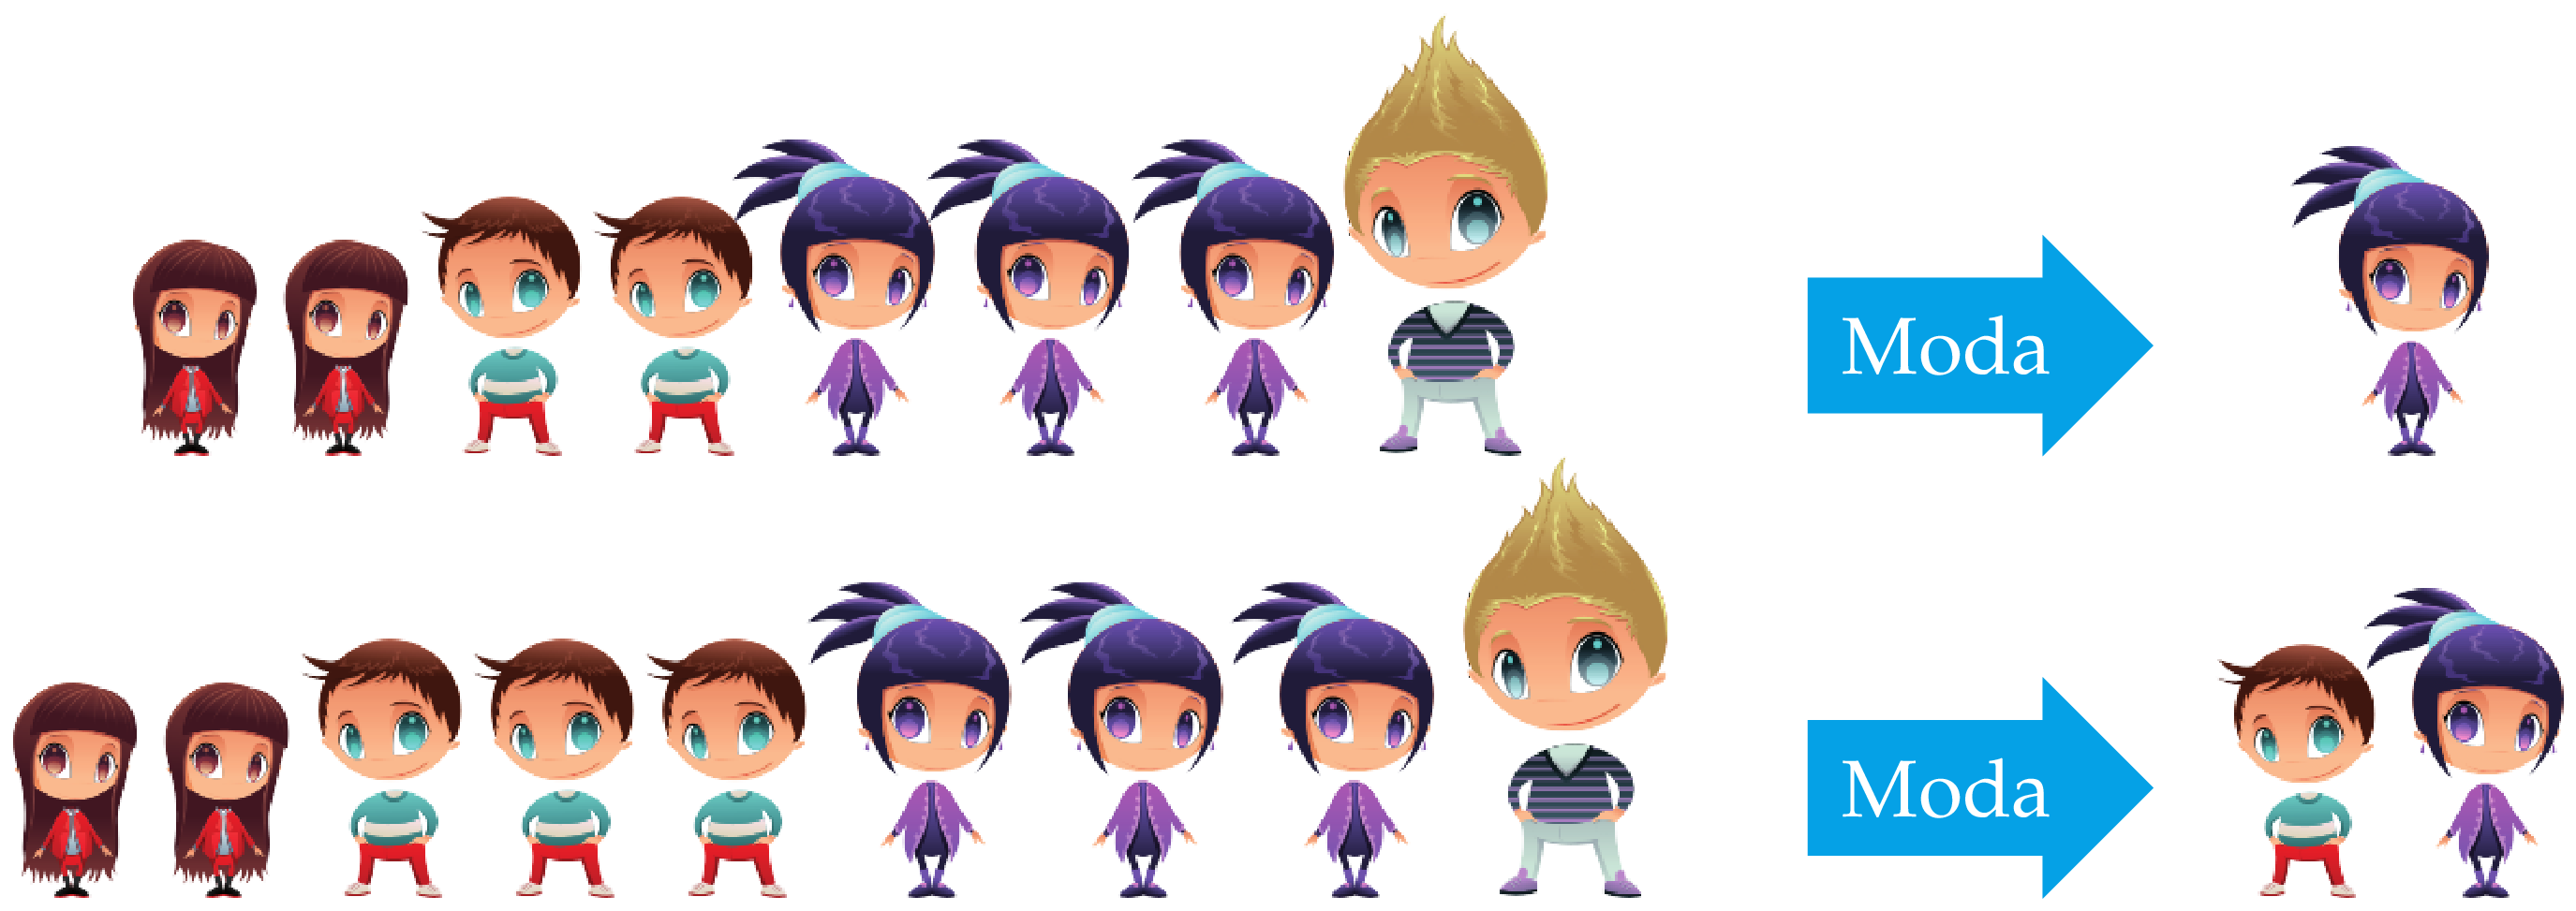
\includegraphics{img/descriptiva/moda.png}

}

\caption{Cálculo de la moda.}

\end{figure}%

\begin{example}[]\protect\hypertarget{exm-moda-datos-no-agrupados}{}\label{exm-moda-datos-no-agrupados}

Utilizando los datos de la muestra del número de hijos en las familias,
el valor con mayor frecuencia es 2, y por tanto la moda es \(Mo=2\).

\[
\begin{array}{rr}
\hline
x_i & n_i \\
\hline
0 & 2 \\
1 & 6 \\
\color{red} 2 & 14 \\
3 & 2  \\
4 & 1 \\
\hline
\end{array}
\]

\end{example}

\begin{example}[]\protect\hypertarget{exm-moda-datos-agrupados}{}\label{exm-moda-datos-agrupados}

Utilizando los datos de la muestra de estaturas de estudiantes, la clase
con la mayor frecuencia es \((170,180]\), que es la clase modal
\(Mo=(170,180]\).

\[
\begin{array}{cr}
\hline
X & n_i \\
\hline
(150,160] & 2 \\
(160,170] & 8 \\
\color{red}{(170,180]} & 11 \\
(180,190] & 7 \\
(190,200] & 2 \\
\hline
\end{array}
\]

\end{example}

\subsection{¿Qué estadístico de tendencia central
usar?}\label{quuxe9-estaduxedstico-de-tendencia-central-usar}

En general, siempre que puedan calcularse los estadísticos de tendencia
central, es recomendable utilizarlos como valores representativos en el
siguiente orden:

\begin{enumerate}
\def\labelenumi{\arabic{enumi}.}
\item
  Media. La media utiliza más información que el resto ya que para
  calcularla se tiene en cuenta la magnitud de los datos.
\item
  Mediana. La mediana utiliza menos información que la media, pero más
  que la moda, ya que para calcularla se tiene en cuenta el orden de los
  datos.
\item
  Moda. La moda es la que menos información utiliza ya que para
  calcularla sólo se tienen en cuenta las frecuencias absolutas.
\end{enumerate}

\begin{tcolorbox}[enhanced jigsaw, title=\textcolor{quarto-callout-warning-color}{\faExclamationTriangle}\hspace{0.5em}{Advertencia}, coltitle=black, colframe=quarto-callout-warning-color-frame, opacitybacktitle=0.6, toprule=.15mm, breakable, opacityback=0, colbacktitle=quarto-callout-warning-color!10!white, colback=white, toptitle=1mm, rightrule=.15mm, bottomrule=.15mm, left=2mm, bottomtitle=1mm, titlerule=0mm, arc=.35mm, leftrule=.75mm]

Hay que tener cuidado con los datos atípicos, ya que la media puede
distorsionarse cuando hay datos atípicos. En tal caso es mejor utilizar
la mediana como valor más representativo.

\end{tcolorbox}

\begin{example}[]\protect\hypertarget{exm-media-mediana-datos-atipicos}{}\label{exm-media-mediana-datos-atipicos}

Si una muestra de número de hijos de 7 familias es

0, 0, 1, 1, 2, 2, 15,

entonces, \(\bar{x}=3\) hijos y \(Me=1\) hijo.

\emph{¿Qué medida representa mejor el número de hijos en la muestra?}

\end{example}

\subsection{Medidas de posición no
centrales}\label{medidas-de-posiciuxf3n-no-centrales}

Las medidas de posición no centrales o \emph{cuantiles} dividen la
distribución en partes iguales.

Los más utilizados son:

\textbf{Cuartiles}: Dividen la distribución en 4 partes iguales. Hay 3
cuartiles: \(C_1\) (25\% acumulado), \(C_2\) (50\% acumulado), \(C_3\)
(75\% acumulado).

\textbf{Deciles}: Dividen la distribución en 10 partes iguales. Hay 9
deciles: \(D_1\) (10\% acumulado),\ldots, \(D_9\) (90\% acumulado).

\textbf{Percentiles}: Dividen la distribución en 100 partes iguales. Hay
99 percentiles: \(P_1\) (1\% acumulado),\ldots, \(P_{99}\) (99\%
acumulado).

\begin{figure}[H]

{\centering 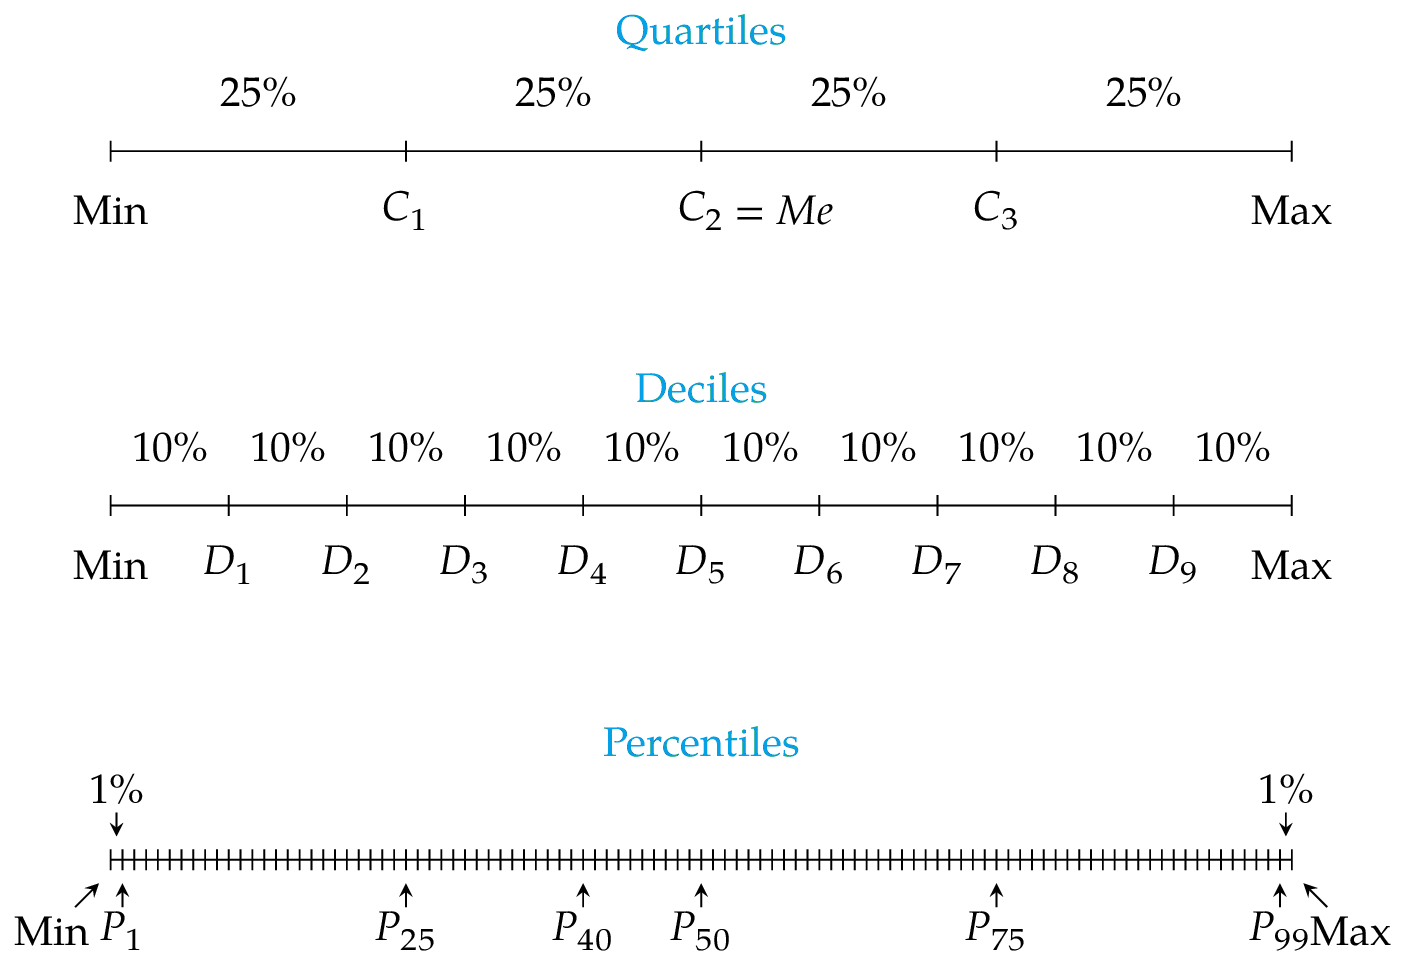
\includegraphics{img/descriptiva/cuantiles.png}

}

\caption{Cuartiles, deciles y percentiles.}

\end{figure}%

Obsérvese que hay una correspondencia entre los cuartiles, los deciles y
los percentiles. Por ejemplo, el primer cuartil coincide con el
percentil 25, y el cuarto decil coincide con el percentil 40.

Los cuantiles se calculan de forma similar a la mediana. La única
diferencia es la frecuencia relativa acumulada que corresponde a cada
cuantil.

\begin{figure}[H]

{\centering 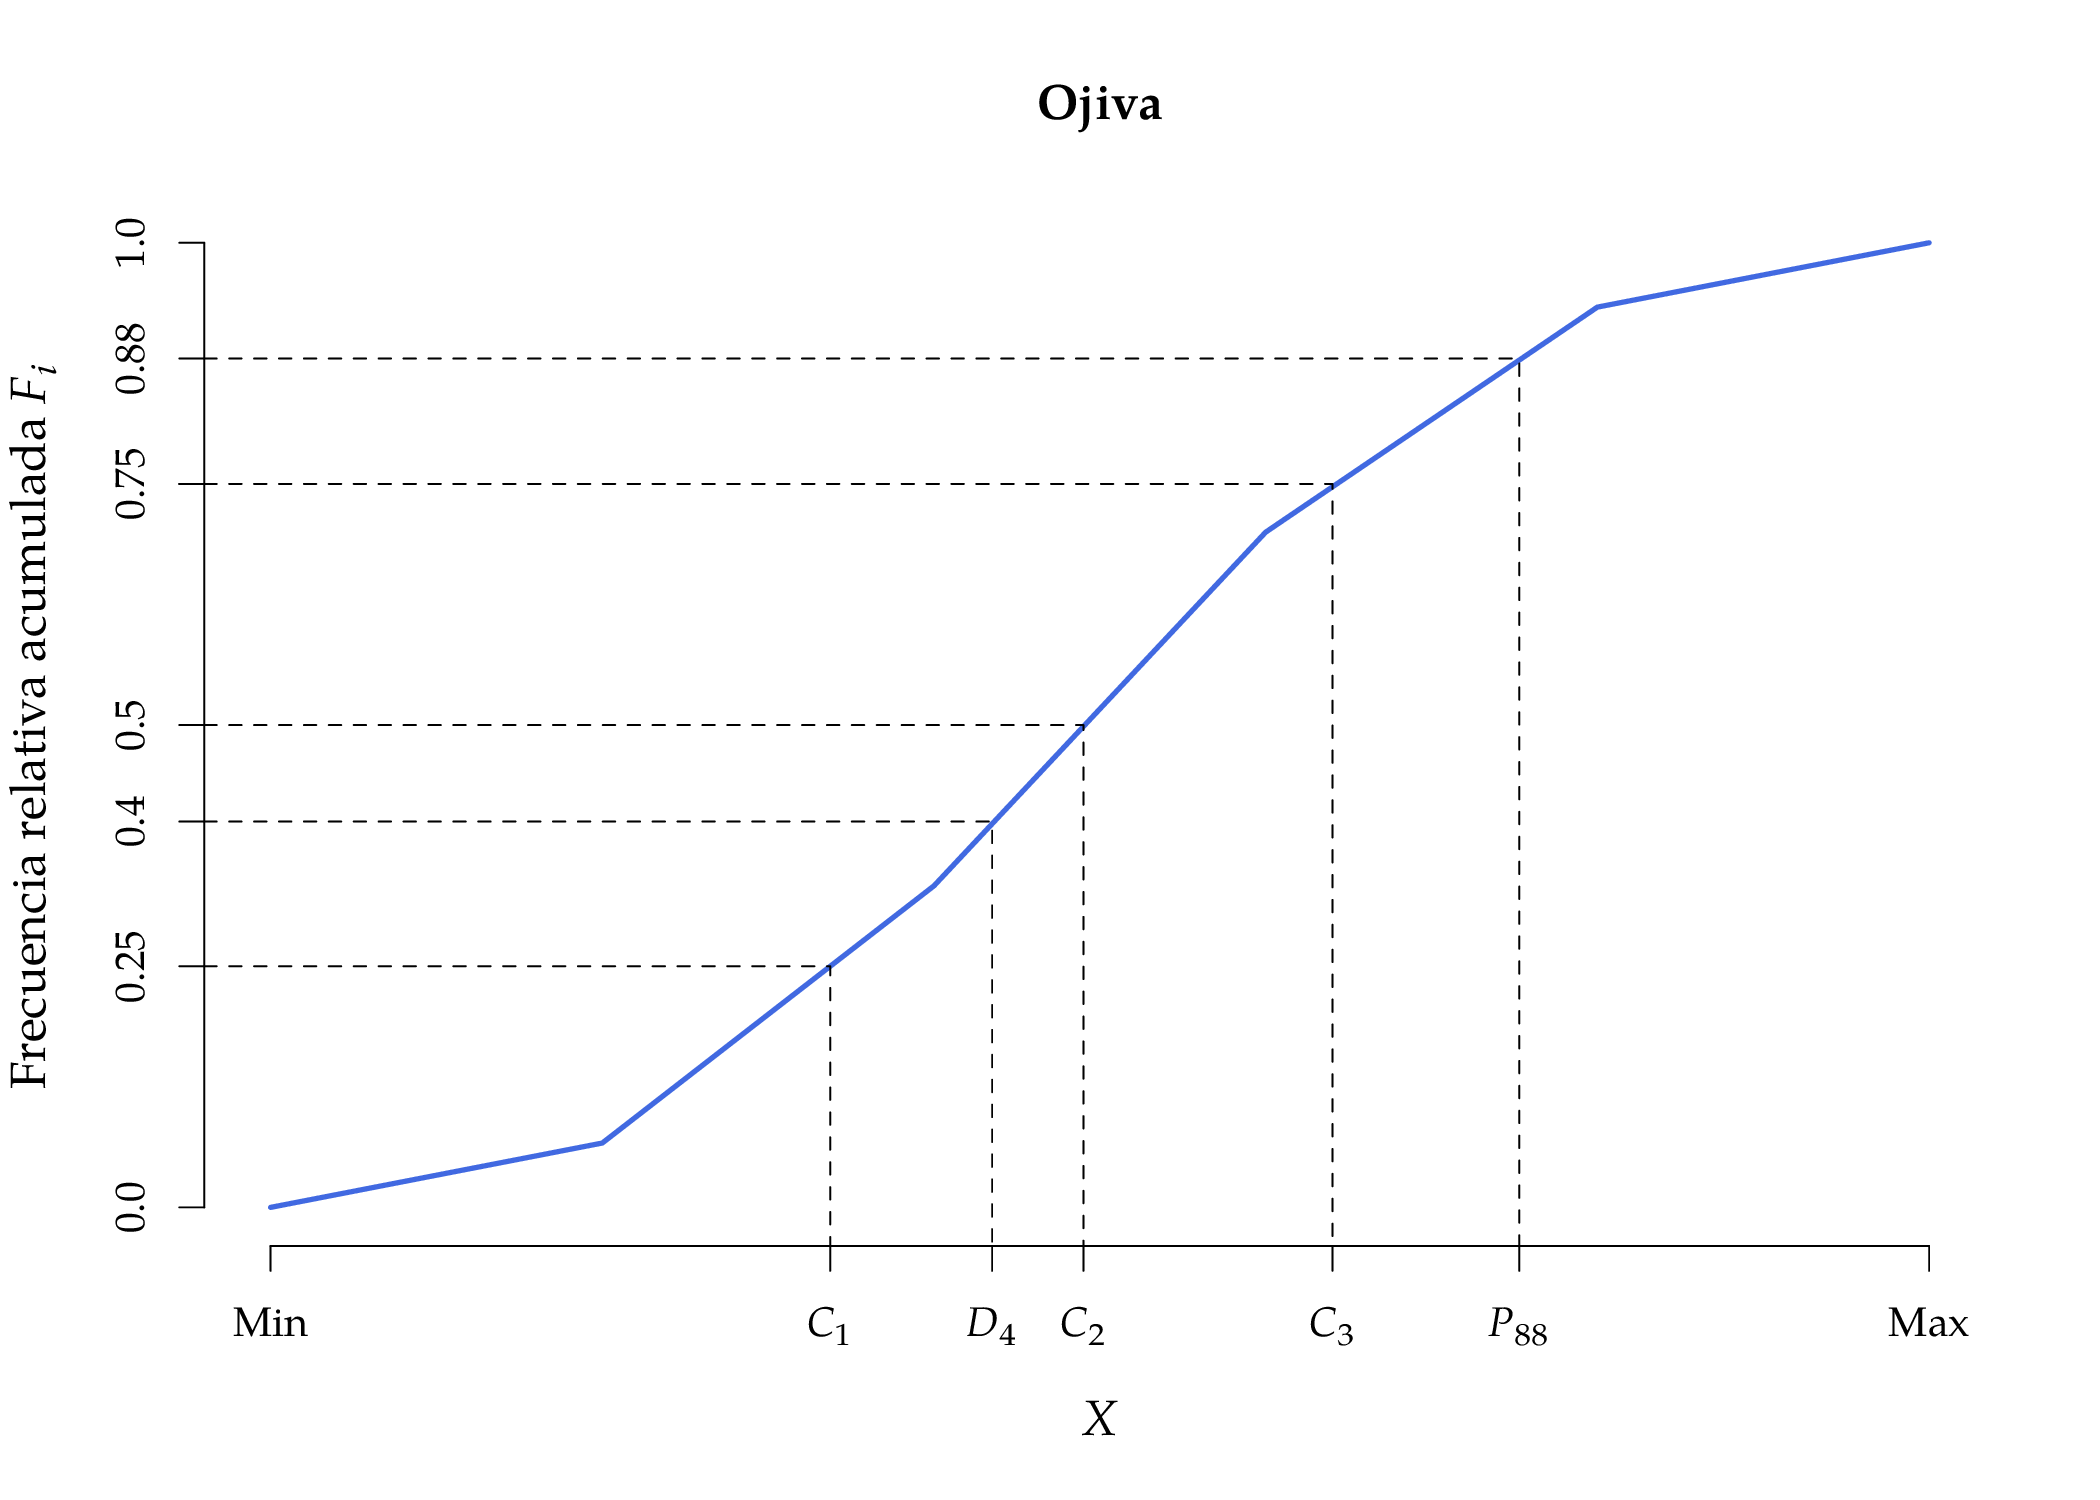
\includegraphics{img/descriptiva/cuantiles_calculo.png}

}

\caption{Cálculo de cuartiles, deciles y percentiles.}

\end{figure}%

\begin{example}[]\protect\hypertarget{exm-cuantiles-datos-no-agrupados}{}\label{exm-cuantiles-datos-no-agrupados}

Utilizando los datos de la muestra del número de hijos de las familias,
la frecuencia relativa acumulada era

\[
\begin{array}{rr}
\hline
x_i & F_i \\
\hline
0 & 0.08\\
1 & 0.32\\
2 & 0.88\\
3 & 0.96\\
4 & 1\\
\hline
\end{array}
\]

\begin{align*}
F_{C_1}=0.25 &\Rightarrow Q_1 = 1 \text{ hijos},\\
F_{C_2}=0.5 &\Rightarrow Q_2 = 2 \text{ hijos},\\
F_{C_3}=0.75 &\Rightarrow Q_3 = 2 \text{ hijos},\\
F_{D_4}=0.4 &\Rightarrow D_4 = 2 \text{ hijos},\\
F_{P_{92}}=0.92 &\Rightarrow P_{92} = 3 \text{ hijos}.
\end{align*}

\end{example}

\section{Estadísticos de
dispersión}\label{estaduxedsticos-de-dispersiuxf3n}

La \emph{dispersión} se refiere a la heterogeneidad o variabilidad de
los datos. Así pues, los estadísticos de dispersión mide la variabilidad
global de los datos, o con respecto a una medida de tendencia central.

Para las variables cuantitativas, las más empleadas son:

\begin{itemize}
\tightlist
\item
  Recorrido.
\item
  Rango Intercuartílico.
\item
  Varianza.
\item
  Desviación Típica.
\item
  Coeficiente de Variación.
\end{itemize}

\subsection{Recorrido}\label{recorrido}

\begin{definition}[Recorrido muestral
\(Re\)]\protect\hypertarget{def-recorrido-muestral}{}\label{def-recorrido-muestral}

El \emph{recorrido muestral} o \emph{rango muestral} de una variable
\(X\) se define como la diferencia entre el máximo y el mínimo de los
valores en la muestra.

\[Re = \max_{x_i} -\min_{x_i}\]

\end{definition}

\begin{figure}[H]

{\centering 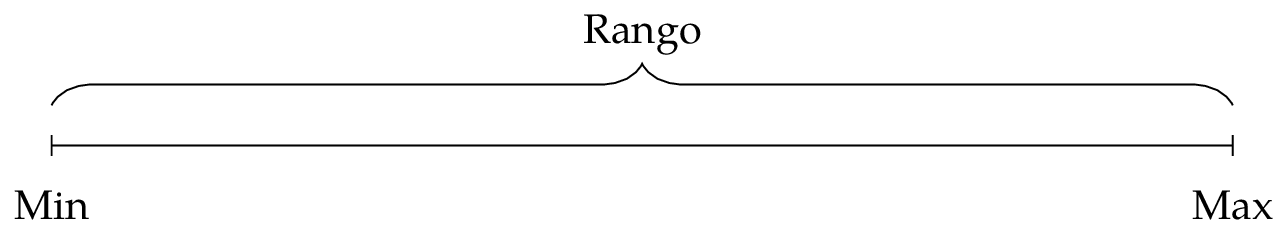
\includegraphics{img/descriptiva/rango.png}

}

\caption{Rango muestral.}

\end{figure}%

El recorrido mide la máxima variación que hay entre los datos
muestrales. No obstante, es muy sensible a datos atípicos ya que suelen
aparecer justo en los extremos de la distribución, por lo que no se
suele utilizar mucho.

\subsection{Rango intercuartílico}\label{rango-intercuartuxedlico}

Para evitar el problema de los datos atípicos en el recorrido, se puede
utilizar el primer y tercer cuartil en lugar del mínimo y el máximo.

\begin{definition}[Rango intercuartílico muestral
\(RI\)]\protect\hypertarget{def-rango-intercuartilico}{}\label{def-rango-intercuartilico}

El \emph{rango intercuartílico muestral} de una variable \(X\) se define
como la diferencia entre el tercer y el primer cuartil de la muestra.

\[RI = C_3 -C_1\]

\end{definition}

\begin{figure}[H]

{\centering 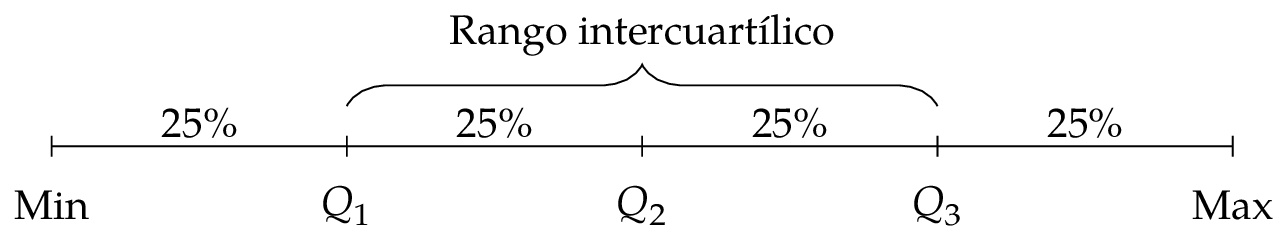
\includegraphics{img/descriptiva/rango_intercuartilico.png}

}

\caption{Rango intercuartílico.}

\end{figure}%

El rango intercuartílico mide la dispersión del 50\% de los datos
centrales.

\subsection{Diagrama de caja y
bigotes}\label{diagrama-de-caja-y-bigotes}

La dispersión de una variable suele representarse gráficamente mediante
un \emph{diagrama de caja y bigotes}, que representa cinco estadísticos
descriptivos (mínimo, cuartiles y máximo) conocidos como los \emph{cinco
números}. Consiste en una caja, dibujada desde el primer al tercer
cuartil, que representa el rango intercuartílico, y dos segmentos,
conocidos como \emph{bigotes} inferior y superior. A menudo la caja se
divide en dos por la mediana.

Este diagrama es muy útil y se utiliza para muchos propósitos:

\begin{itemize}
\tightlist
\item
  Sirve para medir la dispersión de los datos ya que representa el rango
  y el rango intercuartílico.
\item
  Sirve para detectar datos atípicos, que son los valores que quedan
  fuera del intervalo definido por los bigotes.
\item
  Sirve para medir la simetría de la distribución, comparando la
  longitud de las cajas y de los bigotes por encima y por debajo de la
  mediana.
\end{itemize}

:::\{\#exm-diagrama-caja\} El diagrama siguiente muestra el diagrama de
caja y bigotes del peso de una muestra de recién nacidos.

\begin{figure}[H]

{\centering 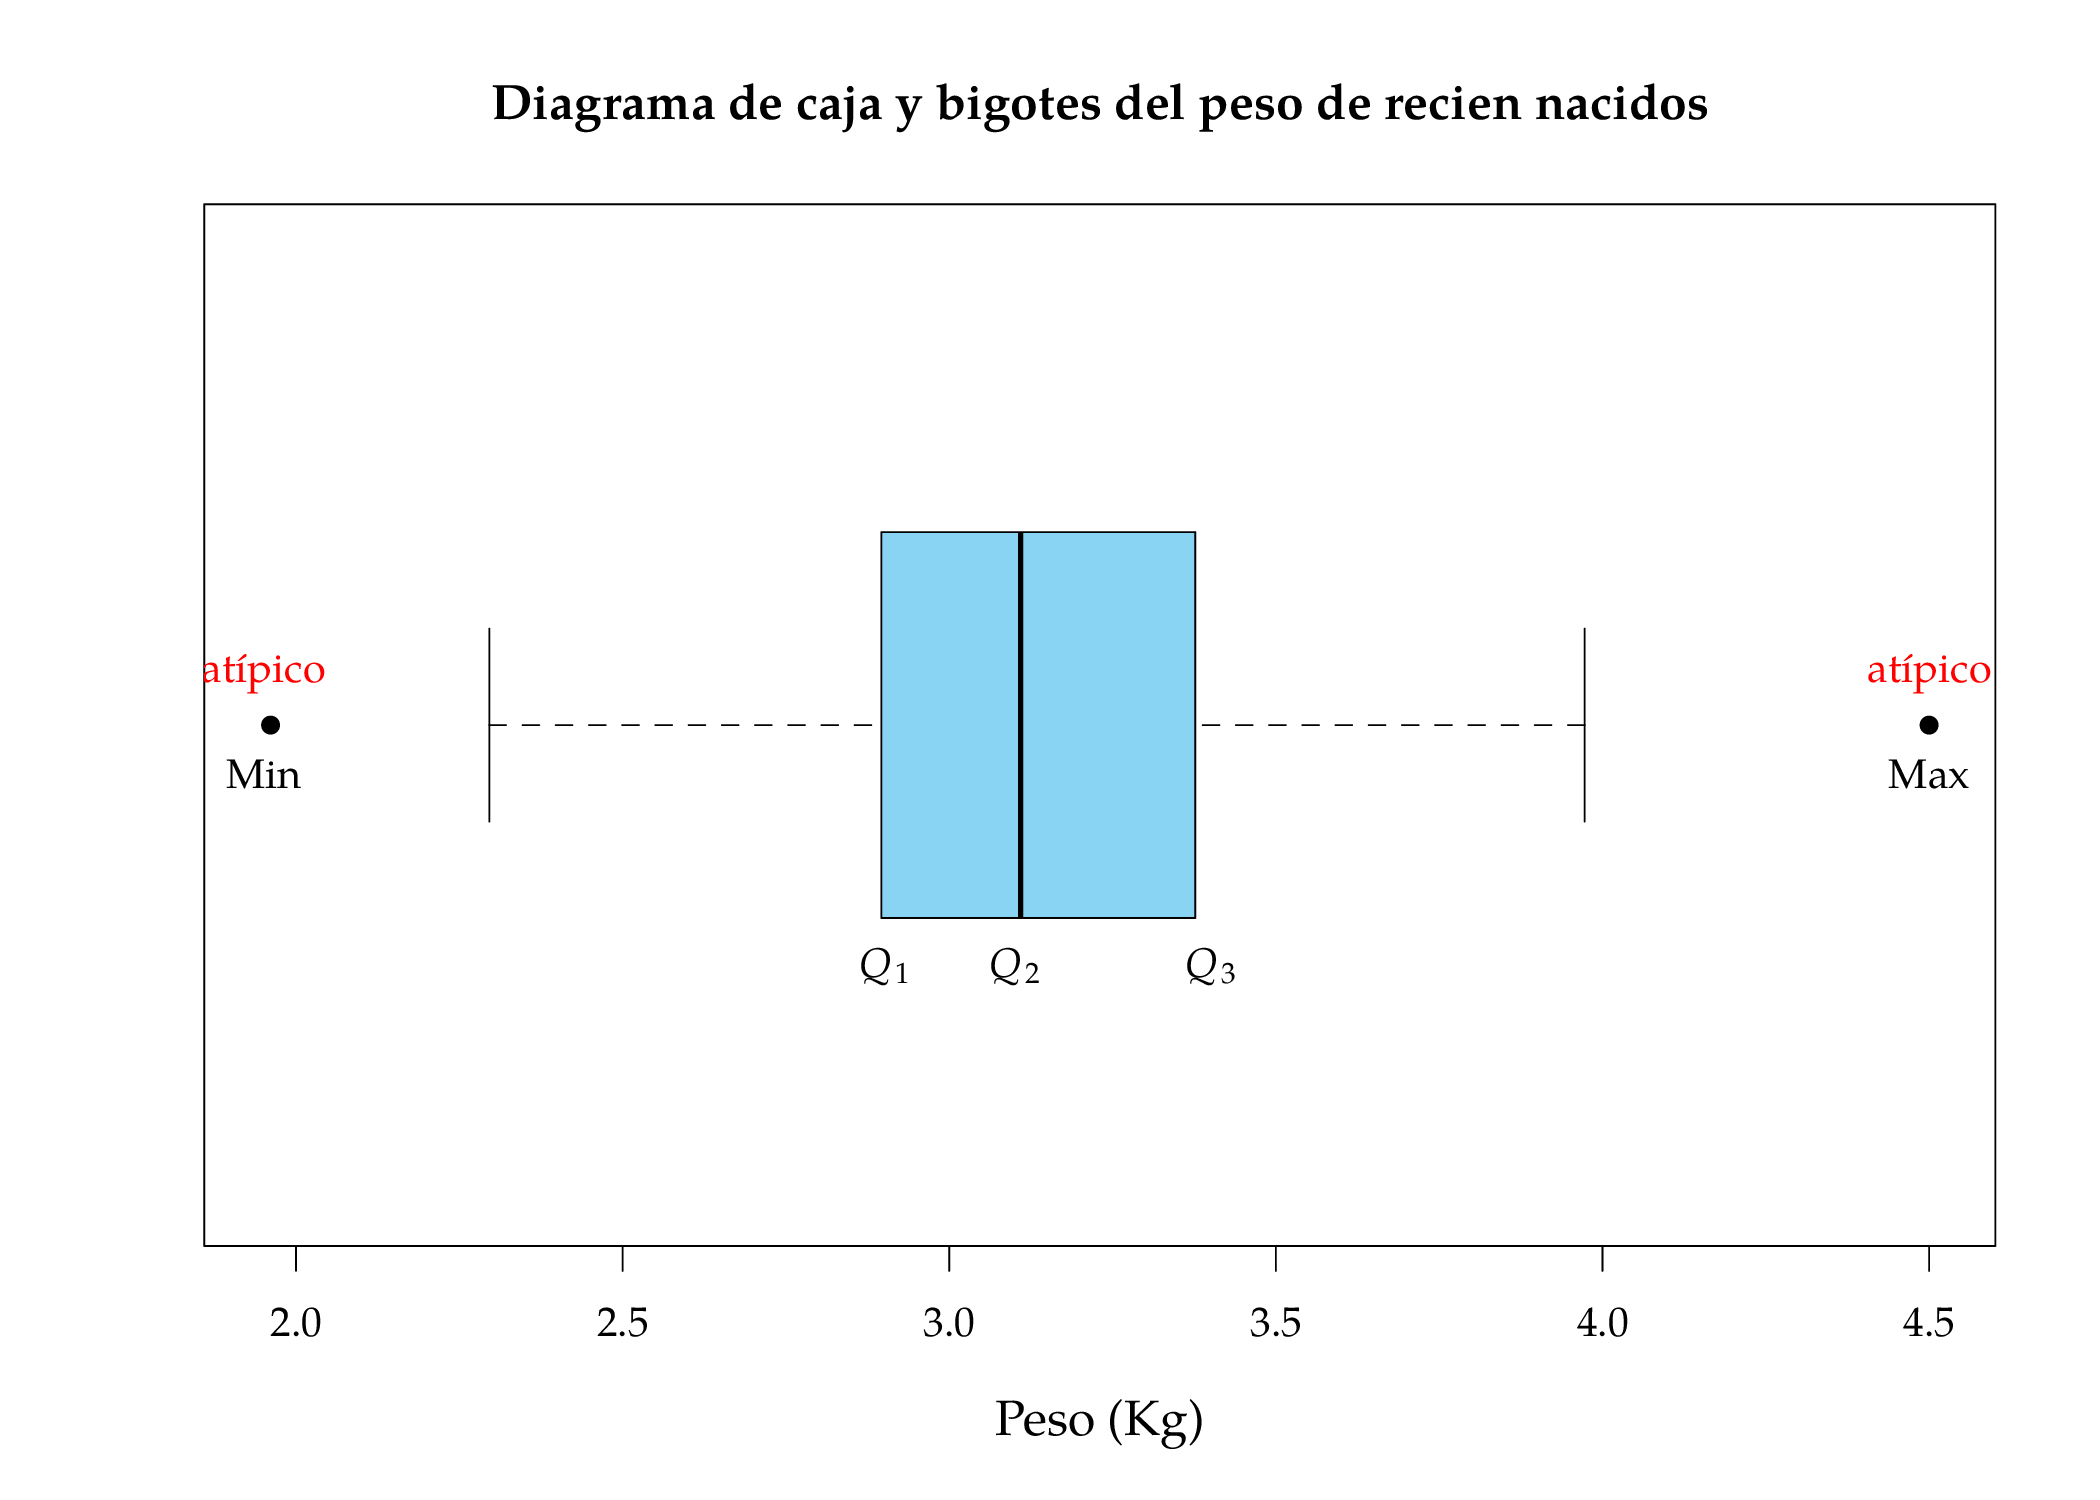
\includegraphics{img/descriptiva/diagrama_caja.png}

}

\caption{Diagrama de caja y bigotes del peso de recién nacidos.}

\end{figure}%

Para construir el diagrama de caja y bigotes hay que seguir los
siguientes pasos:

\begin{enumerate}
\def\labelenumi{\arabic{enumi}.}
\item
  Calcular los cuartiles.
\item
  Dibujar una caja de manera que el extremo inferior caiga sobre el
  primer cuartil y el extremo superior sobre el tercer cuartil.
\item
  Dividir la caja con una línea que caiga sobre el segundo cuartil.
\item
  Para los bigotes inicialmente se calculan dos valores llamados
  \emph{vallas} \(v_1\) y \(v_2\). La valla inferior es el primer
  cuartil menos una vez y media el rango intercuartílico, y la valla
  superior es el tercer cuartil más una vez y media el rango
  intercuartílico.

  \[
   \begin{aligned}
   v_1&=Q_1-1.5\,\text{IQR}\\
   v_2&=Q_3+1.5\,\text{IQR}
   \end{aligned}
   \]

  Las vallas definen el intervalo donde los datos se consideran
  normales. Cualquier valor fuera de ese intervalo se considera un dato
  atípico.\\
  El bigote superior se dibuja desde el borde inferior de la caja hasta
  el menor valor de la muestra que es mayor o igual a la valla inferior,
  y el bigote superior se dibuja desde el borde superior de la caja
  hasta el mayor valor de la muestra que es menor o igual a la valla
  superior.
\end{enumerate}

\begin{tcolorbox}[enhanced jigsaw, title=\textcolor{quarto-callout-warning-color}{\faExclamationTriangle}\hspace{0.5em}{Advertencia}, coltitle=black, colframe=quarto-callout-warning-color-frame, opacitybacktitle=0.6, toprule=.15mm, breakable, opacityback=0, colbacktitle=quarto-callout-warning-color!10!white, colback=white, toptitle=1mm, rightrule=.15mm, bottomrule=.15mm, left=2mm, bottomtitle=1mm, titlerule=0mm, arc=.35mm, leftrule=.75mm]

Los bigotes no son las vallas.

\end{tcolorbox}

\begin{enumerate}
\def\labelenumi{\arabic{enumi}.}
\setcounter{enumi}{4}
\tightlist
\item
  Finalmente, si en la muestra hay algún dato atípico, se dibuja un
  punto para cada uno de ellos.
\end{enumerate}

\begin{example}[]\protect\hypertarget{exm-diagrama-caja}{}\label{exm-diagrama-caja}

El diagrama de caja y bigotes de la muestra del número de hijos de las
familias se muestra a continuación.

\begin{figure}[H]

{\centering 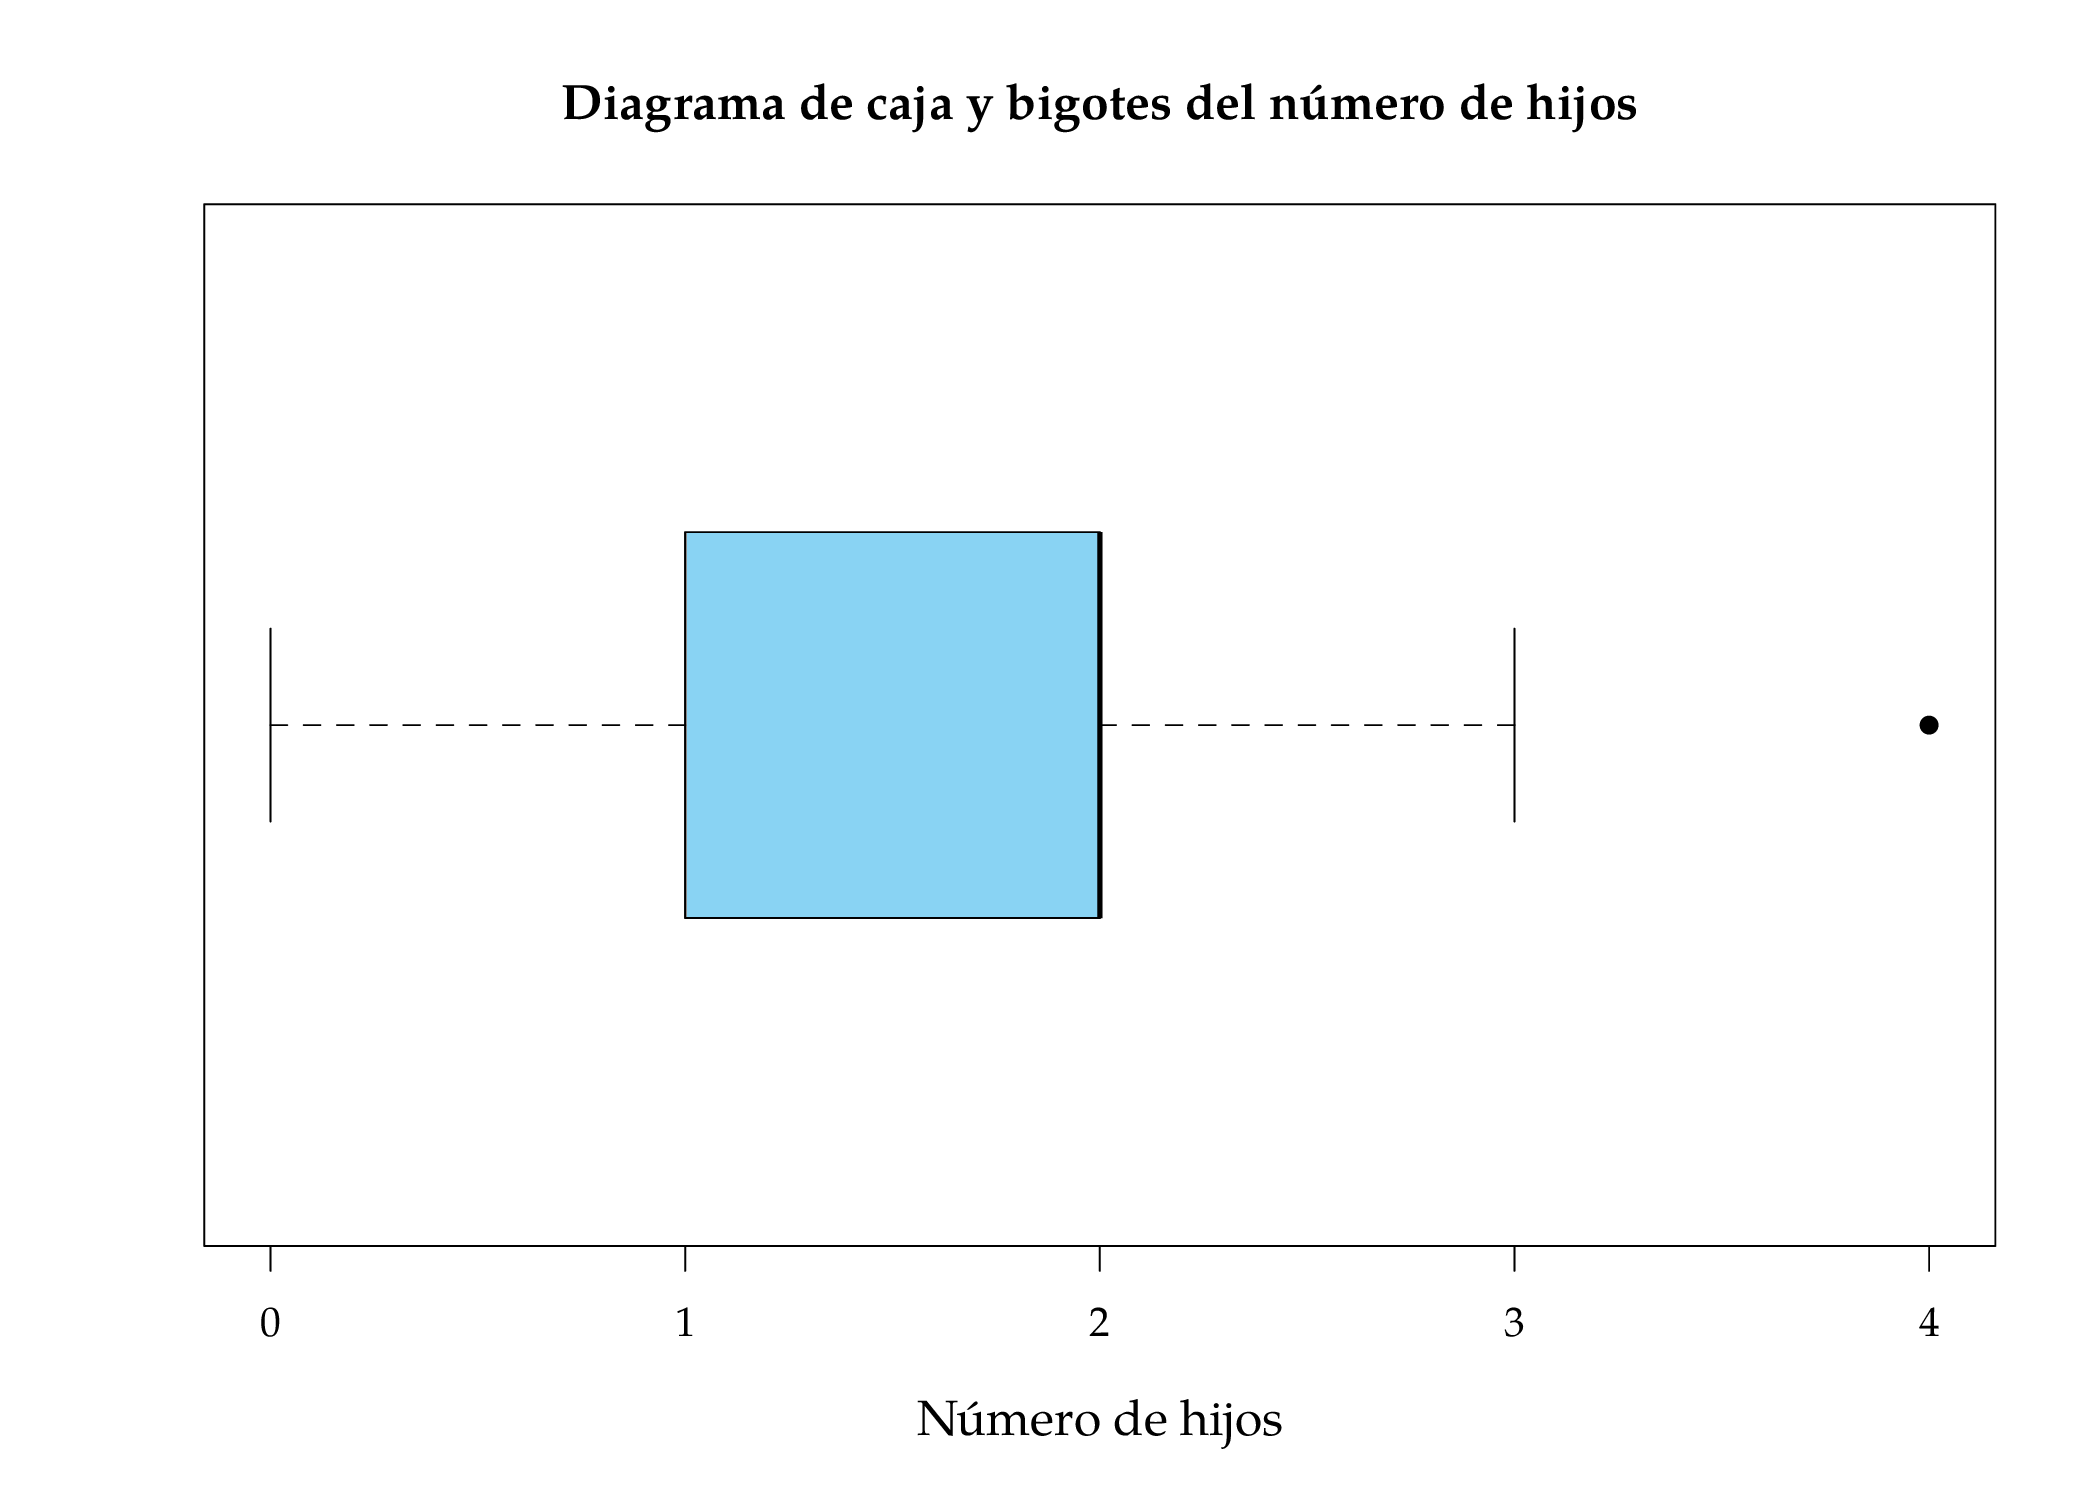
\includegraphics{img/descriptiva/diagrama_caja_hijos.png}

}

\caption{Diagrama de caja y bigotes del número de hijos.}

\end{figure}%

\end{example}

\subsubsection{Desviaciones respecto de la
media}\label{desviaciones-respecto-de-la-media}

Otra forma de medir la variabilidad de una variable es estudiar la
concentración de los valores en torno a algún estadístico de tendencia
central como por ejemplo la media.

Para ello se suele medir la distancia de cada valor a la media. A ese
valor se le llama \textbf{desviación de la media}.

\begin{figure}[H]

{\centering 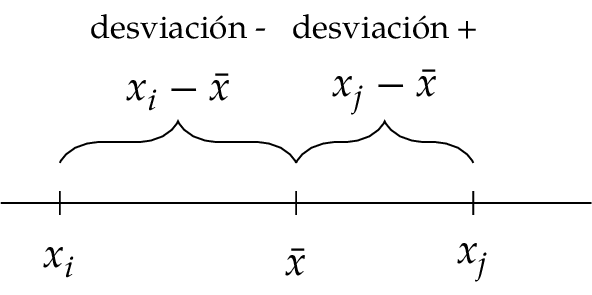
\includegraphics{img/descriptiva/desviaciones.png}

}

\caption{Desviaciones con respecto a la media.}

\end{figure}%

Si las desviaciones son grandes la media no será tan representativa como
cuando la desviaciones sean pequeñas.

\begin{example}[]\protect\hypertarget{exm-desviaciones}{}\label{exm-desviaciones}

La siguiente tabla contiene las notas de 3 estudiantes en un curso con
las asignaturas \(A\), \(B\) y \(C\).

\[
\begin{array}{cccc}
\hline
A & B & C & \bar x \\
0 & 5 & 10 & 5 \\
4 & 5 & 6 & 5 \\
5 & 5 & 5 & 5 \\
\hline
\end{array}
\]

Todos los estudiantes tienen la misma media, pero, en qué caso la media
representa mejor el rendimiento en el curso?

\end{example}

\subsection{Varianza y desviación
típica}\label{varianza-y-desviaciuxf3n-tuxedpica}

\begin{definition}[Varianza
\(s^2\)]\protect\hypertarget{def-varianza}{}\label{def-varianza}

La \emph{varianza muestral} de una variable \(X\) se define como el
promedio del cuadrado de las desviaciones de los valores de la muestra
respecto de la media muestral.

\[s^2 = \frac{\sum (x_i-\bar x)^2n_i}{n} = \sum (x_i-\bar x)^2f_i\]

\end{definition}

También puede calcularse de manera más sencilla mediante la fórmula

\[s^2 = \frac{\sum x_i^2n_i}{n} -\bar x^2= \sum x_i^2f_i-\bar x^2\]

La varianza tiene las unidades de la variable al cuadrado, por lo que
para facilitar su interpretación se suele utilizar su raíz cuadrada.

\begin{definition}[Desviación típica
\(s\)]\protect\hypertarget{def-desviacion-tipica}{}\label{def-desviacion-tipica}

La \emph{desviación típica muestral} de una variable \(X\) se define
como la raíz cuadrada positiva de su varianza muestral.

\[s = +\sqrt{s^2}\]

\end{definition}

\begin{tcolorbox}[enhanced jigsaw, title=\textcolor{quarto-callout-tip-color}{\faLightbulb}\hspace{0.5em}{Tip}, coltitle=black, colframe=quarto-callout-tip-color-frame, opacitybacktitle=0.6, toprule=.15mm, breakable, opacityback=0, colbacktitle=quarto-callout-tip-color!10!white, colback=white, toptitle=1mm, rightrule=.15mm, bottomrule=.15mm, left=2mm, bottomtitle=1mm, titlerule=0mm, arc=.35mm, leftrule=.75mm]

Tanto la varianza como la desviación típica sirven para cuantificar la
dispersión de los datos en torno a la media. Cuando la varianza o la
desviación típica son pequeñas, los datos de la muestra están
concentrados en torno a la media, y la media es una buena medida de
representatividad. Por contra, cuando la varianza o la desviación típica
son grandes, los datos de la muestra están alejados de la media, y la
media ya no representa tan bien.

\begin{longtable}[]{@{}lcl@{}}
\toprule\noalign{}
\endhead
\bottomrule\noalign{}
\endlastfoot
Desviación típica pequeña & \(\Rightarrow\) & Media representativa \\
Desviación típica grande & \(\Rightarrow\) & Media no representativa \\
\end{longtable}

\end{tcolorbox}

\begin{example}[]\protect\hypertarget{exm-intrepretacion-desviacion-tipica}{}\label{exm-intrepretacion-desviacion-tipica}

Las siguientes muestras contienen las notas de dos estudiantes en dos
asignaturas.

\begin{figure}[H]

{\centering 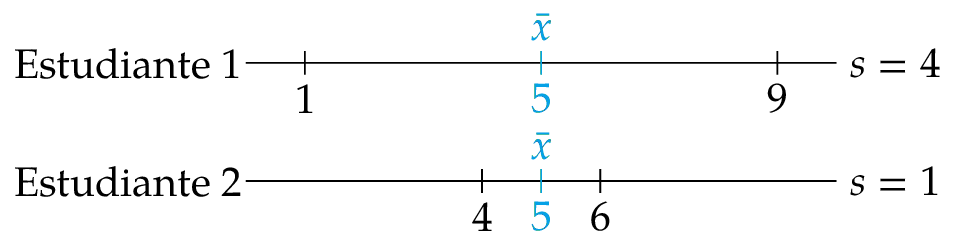
\includegraphics{img/descriptiva/interpretacion_desviacion_tipica.png}

}

\caption{Interpretación de la desviación típica.}

\end{figure}%

\emph{¿Qué media es más representativa?}

\end{example}

\begin{example}[Datos no
agrupados]\protect\hypertarget{exm-desviacion-tipica-datos-no-agrupados}{}\label{exm-desviacion-tipica-datos-no-agrupados}

Utilizando los datos de la muestra del número de hijos de las familias,
con una media \(\bar x=1.76\) hijos, y añadiendo una nueva columna a la
tabla de frecuencias con los cuadrados de los valores,

\[
\begin{array}{rrr}
\hline
x_i & n_i & x_i^2n_i \\
\hline
0 & 2 & 0 \\
1 & 6 & 6 \\
2 & 14 & 56\\
3 & 2  & 18\\
4 & 1 & 16 \\
\hline
\sum & 25 & 96 \\
\hline
\end{array}\]

\[s^2 = \frac{\sum x_i^2n_i}{n}-\bar x^2 = \frac{96}{25}-1.76^2= 0.7424 \mbox{ hijos}^2.\]

y la desviación típica es \(s=\sqrt{0.7424} = 0.8616\) hijos.

Comparado este valor con el recorrido, que va de 0 a 4 hijos se observa
que no es demasiado grande por lo que se puede concluir que no hay mucha
dispersión y en consecuencia la media de \(1.76\) hijos representa bien
el número de hijos de las familias de la muestra.

\end{example}

\begin{example}[Datos
agrupados]\protect\hypertarget{exm-desviacion-tipica-datos-agrupados}{}\label{exm-desviacion-tipica-datos-agrupados}

Utilizando los datos de la muestra de estaturas de los estudiantes y
agrupando las estaturas en clases, se obtenía una media
\(\bar x = 174.67\) cm. El cálculo de la varianza se realiza igual que
antes pero tomando como valores de la variable las marcas de clase.

\[
\begin{array}{crrr}
\hline
X & x_i & n_i & x_i^2n_i \\
\hline
(150,160] & 155 & 2 & 48050\\
(160,170] & 165 & 8 & 217800\\
(170,180] & 175 & 11 & 336875\\
(180,190] & 185 & 7 & 239575\\
(190,200] & 195 & 2 & 76050\\
\hline
\sum &  & 30 & 918350 \\
\hline
\end{array}
\]

\[s^2 = \frac{\sum x_i^2n_i}{n}-\bar x^2 = \frac{918350}{30}-174.67^2= 102.06 \mbox{ cm}^2,\]

y la desviación típica es \(s=\sqrt{102.06} = 10.1\) cm.

Este valor es bastante pequeño, comparado con el recorrido de la
variable, que va de 150 a 200 cm, por lo que la variable tiene poca
dispersión y en consecuencia su media es muy representativa.

\end{example}

\subsection{Coeficiente de variación}\label{coeficiente-de-variaciuxf3n}

Tanto la varianza como la desviación típica tienen unidades y eso
dificulta a veces su interpretación, especialmente cuando se compara la
dispersión de variables con diferentes unidades.

Por este motivo, es también común utilizar la siguiente medida de
dispersión que no tiene unidades.

\begin{definition}[Coeficiente de variación muestral
\(cv\)]\protect\hypertarget{def-coeficiente-variacion}{}\label{def-coeficiente-variacion}

El \emph{coeficiente de variación muestral} de una variable \(X\) se
define como el cociente entre su desviación típica muestral y el valor
absoluto de su media muestral.

\[cv = \frac{s}{|\bar x|}\]

\end{definition}

\begin{tcolorbox}[enhanced jigsaw, title=\textcolor{quarto-callout-tip-color}{\faLightbulb}\hspace{0.5em}{Tip}, coltitle=black, colframe=quarto-callout-tip-color-frame, opacitybacktitle=0.6, toprule=.15mm, breakable, opacityback=0, colbacktitle=quarto-callout-tip-color!10!white, colback=white, toptitle=1mm, rightrule=.15mm, bottomrule=.15mm, left=2mm, bottomtitle=1mm, titlerule=0mm, arc=.35mm, leftrule=.75mm]

El coeficiente de variación muestral mide la dispersión relativa de los
valores de la muestra en torno a la media muestral.

Como no tiene unidades, es muy sencillo de interpretar: Cuanto mayor
sea, mayor será la dispersión relativa con respecto a la media y menos
representativa será la media.

\end{tcolorbox}

El coeficiente de variación es muy útil para comparar la dispersión de
distribuciones de variables diferentes, incluso si las variables tienen
unidades diferentes.

\begin{example}[]\protect\hypertarget{exm-coeficiente-variacion}{}\label{exm-coeficiente-variacion}

En la muestra del número de hijos, donde la media era \(\bar x=1.76\)
hijos y la desviación típica \(s=0.8616\) hijos, el coeficiente de
variación vale

\[cv = \frac{s}{|\bar x|} = \frac{0.8616}{|1.76|} = 0.49.\]

En la muestra de las estaturas, donde la media era \(\bar x=174.67\) cm
y la desviación típica \(s=10.1\) cm, el coeficiente de variación vale

\[cv = \frac{s}{|\bar x|} = \frac{10.1}{|174.67|} = 0.06.\]

Esto significa que la dispersión relativa en la muestra de estaturas es
mucho menor que en la del número de hijos, por lo que la media de las
estaturas será más representativa que la media del número de hijos.

\end{example}

\section{Estadísticos de forma}\label{estaduxedsticos-de-forma}

Son medidas que describen la forma de la distribución.

Los aspectos más relevantes son:

\textbf{Simetría} Mide la simetría de la distribución de frecuencias en
torno a la media. El estadístico más utilizado es el \emph{Coeficiente
de Asimetría de Fisher}.

\textbf{Apuntamiento} Mide el apuntamiento o el grado de concentración
de valores en torno a la media de la distribución de frecuencias. El
estadístico más utilizado es el \emph{Coeficiente de Apuntamiento o
Curtosis}.

\subsection{Coeficiente de asimetría}\label{coeficiente-de-asimetruxeda}

\begin{definition}[Coeficiente de asimetría muestral
\(g_1\)]\protect\hypertarget{def-coeficiente-asimetria}{}\label{def-coeficiente-asimetria}

El \emph{coeficiente de asimetría muestral} de una variable \(X\) es el
promedio de las desviaciones de los valores de la muestra respecto de la
media muestral, elevadas al cubo, dividido por la desviación típica al
cubo.

\[g_1 = \frac{\sum (x_i-\bar x)^3 n_i/n}{s^3} = \frac{\sum (x_i-\bar x)^3 f_i}{s^3}\]

\end{definition}

\begin{tcolorbox}[enhanced jigsaw, title=\textcolor{quarto-callout-tip-color}{\faLightbulb}\hspace{0.5em}{Tip}, coltitle=black, colframe=quarto-callout-tip-color-frame, opacitybacktitle=0.6, toprule=.15mm, breakable, opacityback=0, colbacktitle=quarto-callout-tip-color!10!white, colback=white, toptitle=1mm, rightrule=.15mm, bottomrule=.15mm, left=2mm, bottomtitle=1mm, titlerule=0mm, arc=.35mm, leftrule=.75mm]

Mide el grado de simetría de los valores de la muestra con respecto a la
media muestra, es decir, cuantos valores de la muestra están por encima
o por debajo de la media y cómo de alejados de esta.

\begin{itemize}
\tightlist
\item
  \(g_1=0\) indica que hay el mismo número de valores por encima y por
  debajo de la media e igualmente alejados de ella (simétrica).
\end{itemize}

\begin{figure}[H]

{\centering 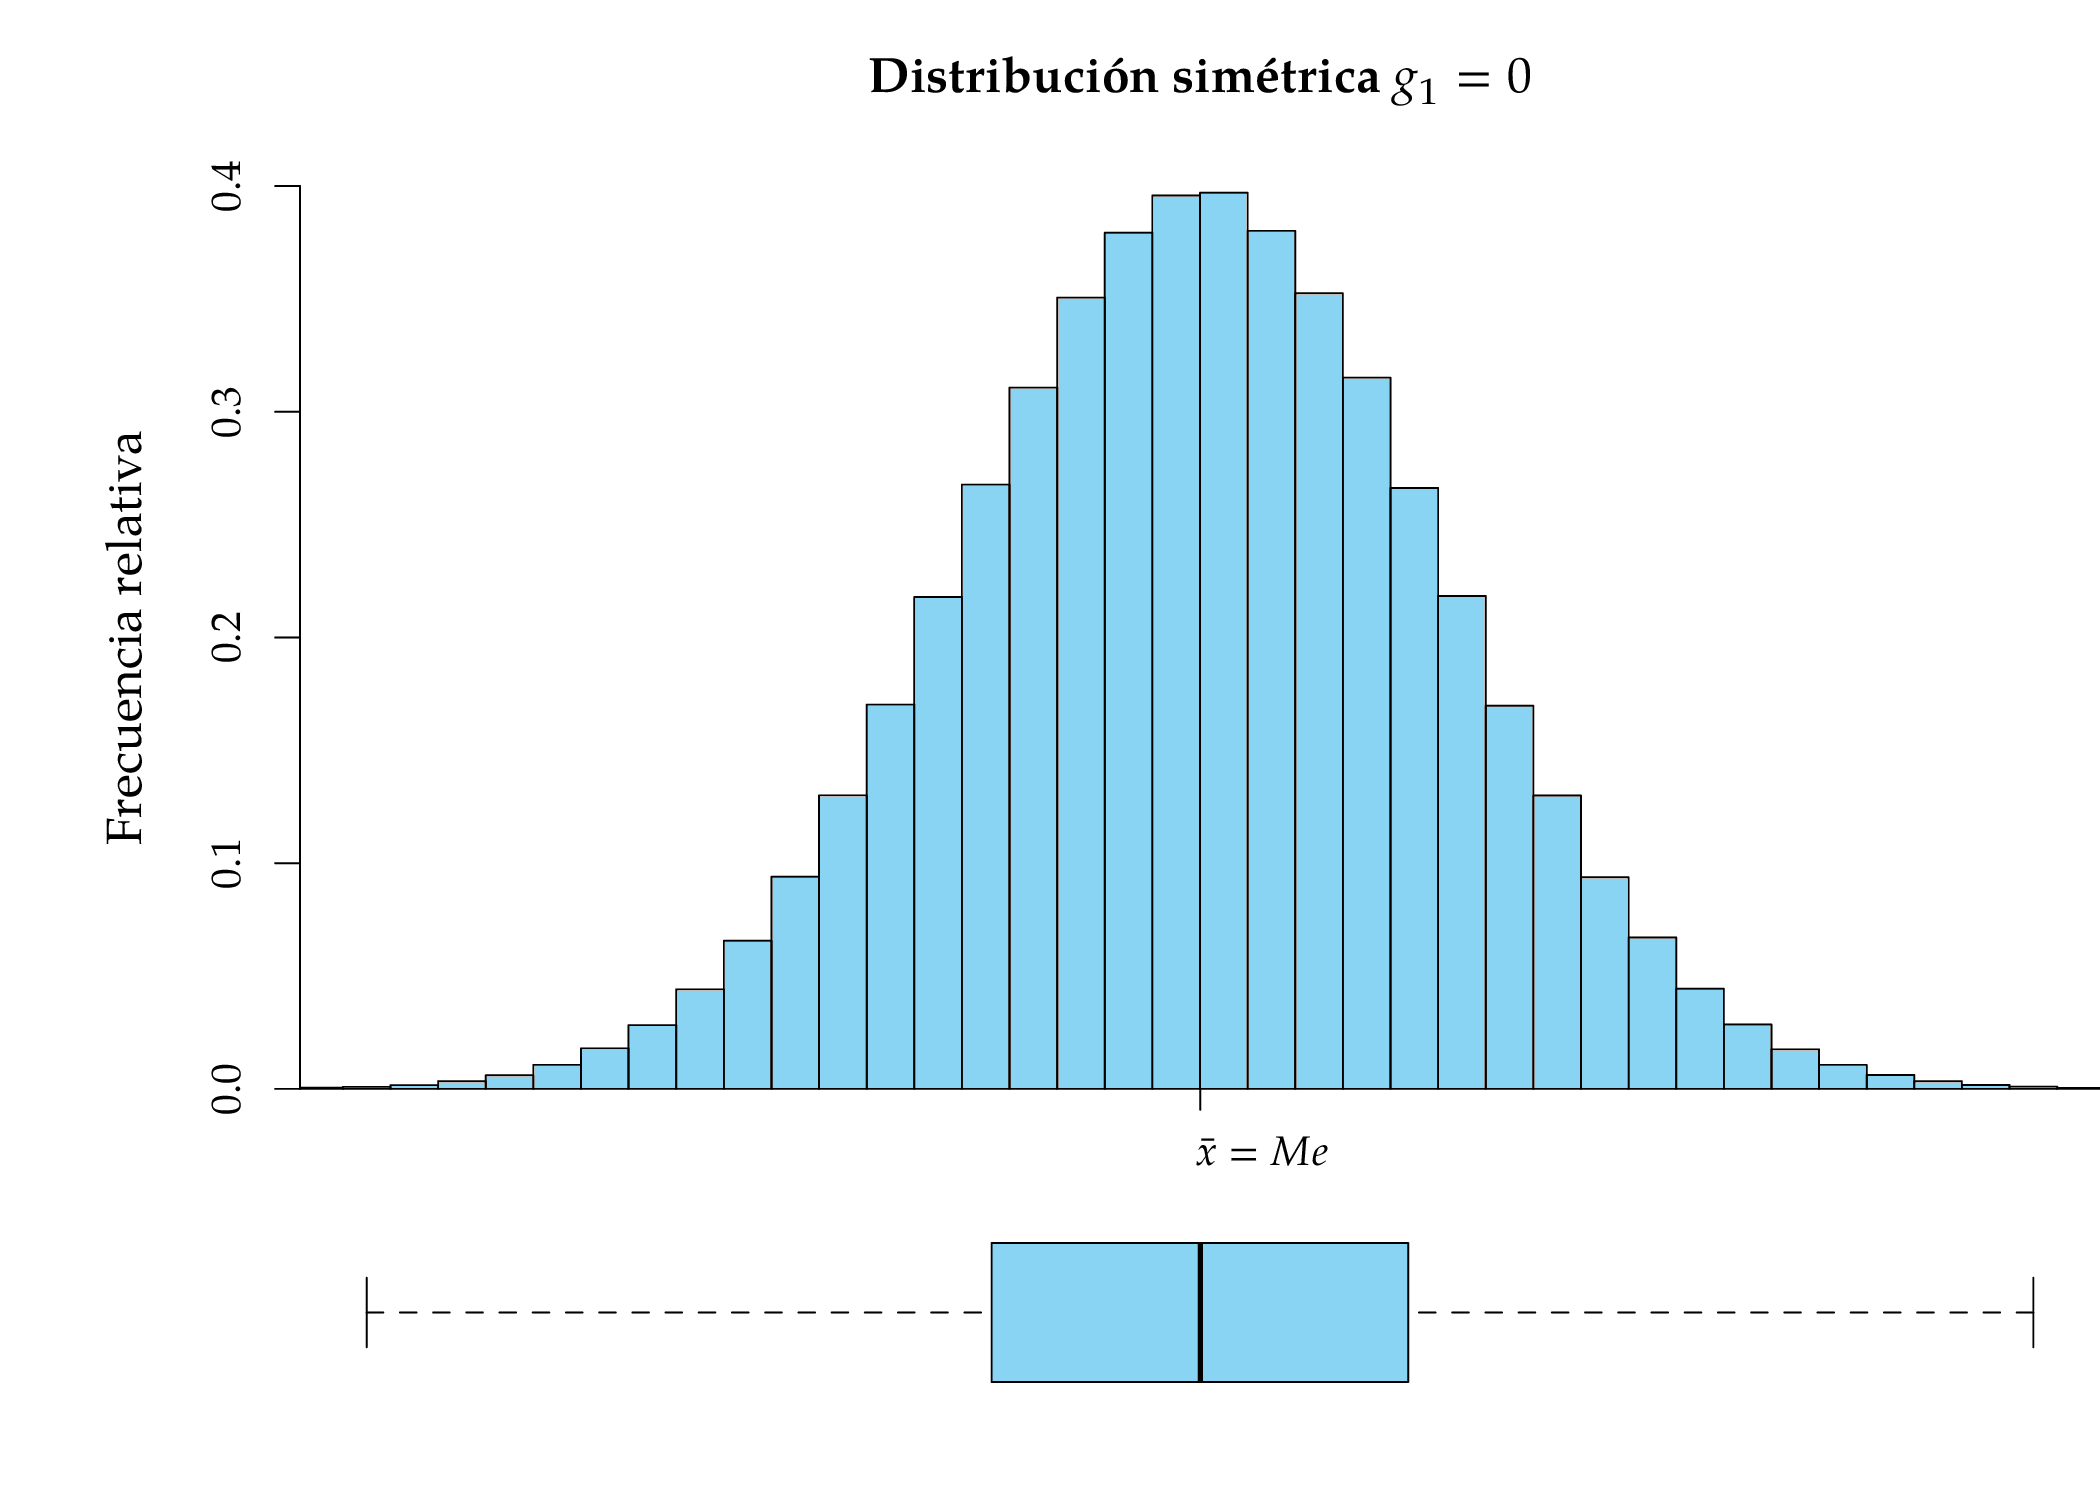
\includegraphics{img/descriptiva/distribucion_simetrica.png}

}

\caption{Distribución simétrica.}

\end{figure}%

\begin{itemize}
\tightlist
\item
  \(g_1<0\) indica que la mayoría de los valores son mayores que la
  media, pero los valores menores están más alejados de ella (asimétrica
  a la izquierda).
\end{itemize}

\begin{figure}[H]

{\centering 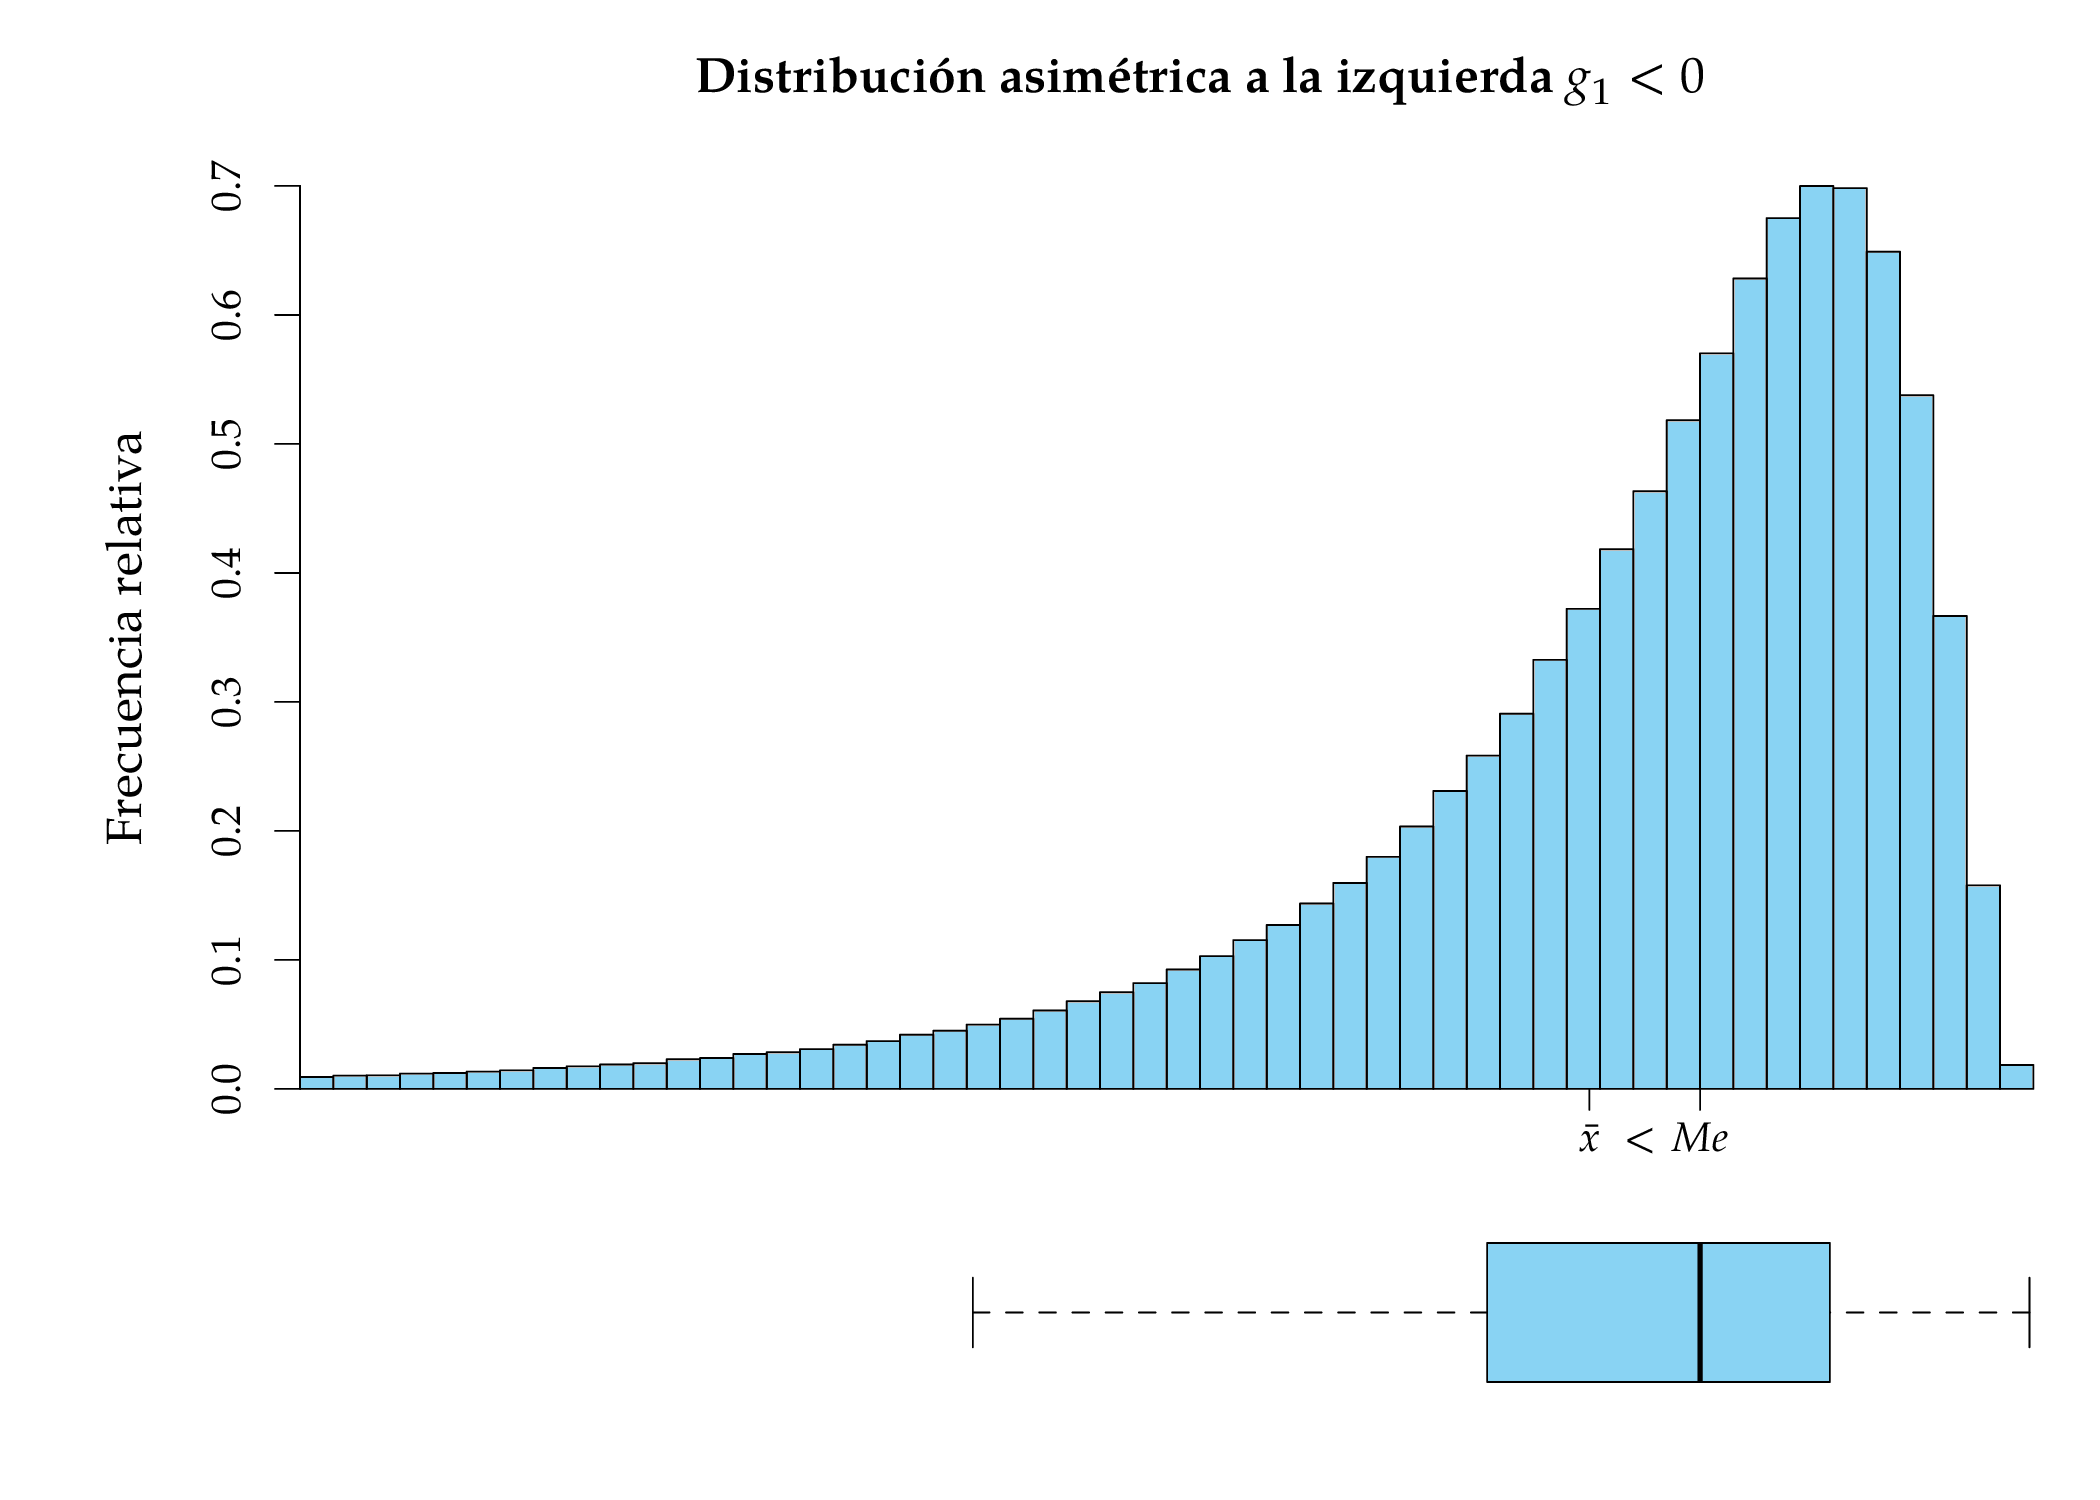
\includegraphics{img/descriptiva/distribucion_asimetrica_izquierda.png}

}

\caption{Distribución asimétrica hacia la izquierda.}

\end{figure}%

\begin{itemize}
\tightlist
\item
  \(g_1>0\) indica que la mayoría de los valores son menores que la
  media, pero los valores mayores están más alejados de ella (asimétrica
  a la derecha).
\end{itemize}

\begin{figure}[H]

{\centering \includegraphics{img/descriptiva/distribucion_asimetrica_derecha.png}

}

\caption{Distribución asimétrica hacia la derecha.}

\end{figure}%

\end{tcolorbox}

\begin{example}[Datos
agrupados]\protect\hypertarget{exm-coeficiente-asimetria}{}\label{exm-coeficiente-asimetria}

Utilizando la tabla de frecuencias de la muestra de estaturas y
añadiendo una nueva columna con las desviaciones de la media
\(\bar x = 174.67\) cm al cubo, se tiene

\[
\begin{array}{crrrr}
\hline
X & x_i & n_i & x_i-\bar x & (x_i-\bar x)^3 n_i \\
\hline
(150,160] & 155 & 2 & -19.67 & -15221.00\\
(160,170] & 165 & 8 & -9.67 & -7233.85\\
(170,180] & 175 & 11 & 0.33 & 0.40\\
(180,190] & 185 & 7 & 10.33 & 7716.12\\
(190,200] & 195 & 2 & 20.33 & 16805.14\\
\hline
\sum &  & 30 & & 2066.81 \\
\hline
\end{array}
\]

\[g_1 = \frac{\sum (x_i-\bar x)^3n_i/n}{s^3} = \frac{2066.81/30}{10.1^3} = 0.07.\]

Como está cerca de 0, eso significa que la distribución de las estaturas
es casi simétrica.

\end{example}

\subsection{Coeficiente de apuntamiento o
curtosis}\label{coeficiente-de-apuntamiento-o-curtosis}

\begin{definition}[Coeficiente de apuntamiento muestral
\(g_2\)]\protect\hypertarget{def-coeficiente-apuntamiento}{}\label{def-coeficiente-apuntamiento}

El \emph{coeficiente de apuntamiento muestral} de una variable \(X\) es
el promedio de las desviaciones de los valores de la muestra respecto de
la media muestral, elevadas a la cuarta, dividido por la desviación
típica a la cuarta y al resultado se le resta 3.

\[g_2 = \frac{\sum (x_i-\bar x)^4 n_i/n}{s^4}-3 = \frac{\sum (x_i-\bar x)^4 f_i}{s^4}-3\]

\end{definition}

\begin{tcolorbox}[enhanced jigsaw, title=\textcolor{quarto-callout-tip-color}{\faLightbulb}\hspace{0.5em}{Tip}, coltitle=black, colframe=quarto-callout-tip-color-frame, opacitybacktitle=0.6, toprule=.15mm, breakable, opacityback=0, colbacktitle=quarto-callout-tip-color!10!white, colback=white, toptitle=1mm, rightrule=.15mm, bottomrule=.15mm, left=2mm, bottomtitle=1mm, titlerule=0mm, arc=.35mm, leftrule=.75mm]

El coeficiente de apuntamiento mide la concentración de valores en torno
a la media y la longitud de las colas de la distribución. Se toma como
referencia la distribución normal (campana de Gauss).

\begin{itemize}
\tightlist
\item
  \(g_2=0\) indica que la distribución tienen un apuntamiento normal, es
  decir, la concentración de valores en torno a la media es similar al
  de una campana de Gauss (\emph{mesocúrtica}).
\end{itemize}

\begin{figure}[H]

{\centering \includegraphics{img/descriptiva/distribucion_mesocurtica.png}

}

\caption{Distribución mesocúrtica.}

\end{figure}%

\begin{itemize}
\tightlist
\item
  \(g_2<0\) indica que la distribución tiene menos apuntamiento de lo
  normal, es decir, la concentración de valores en torno a la media es
  menor que en una campana de Gauss (\emph{platicúrtica}).
\end{itemize}

\begin{figure}[H]

{\centering \includegraphics{img/descriptiva/distribucion_platicurtica.png}

}

\caption{Distribución platicúrtica.}

\end{figure}%

\begin{itemize}
\tightlist
\item
  \(g_2>0\) indica que la distribución tiene más apuntamiento de lo
  normal, es decir, la concentración de valores en torno a la media es
  menor que en una campana de Gauss (\emph{leptocúrtica}).
\end{itemize}

\begin{figure}[H]

{\centering \includegraphics{img/descriptiva/distribucion_leptocurtica.png}

}

\caption{Distribución leptocúrtica.}

\end{figure}%

\end{tcolorbox}

:::\{\#exm-coeficiente-apuntamiento\} \#\# Datos agrupados Utilizando la
tabla de frecuencias de la muestra de estaturas y añadiendo una nueva
columna con las desviaciones de la media \(\bar x = 174.67\) cm a la
cuarta, se tiene

\[
\begin{array}{rrrrr}
\hline
X & x_i & n_i & x_i-\bar x & (x_i-\bar x)^4 n_i\\
\hline
(150,160] & 155 & 2 & -19.67 & 299396.99\\
(160,170] & 165 & 8 & -9.67 & 69951.31\\
(170,180] & 175 & 11 & 0.33 & 0.13\\
(180,190] & 185 & 7 & 10.33 & 79707.53\\
(190,200] & 195 & 2 & 20.33 & 341648.49\\
\hline
\sum &  & 30 & & 790704.45 \\
\hline
\end{array}
\]

\[g_2 = \frac{\sum (x_i-\bar x)^4n_i/n}{s^4} - 3 = \frac{790704.45/30}{10.1^4}-3 = -0.47.\]

Como se trata de un valor negativo, aunque cercano a 0, podemos decir
que la distribución es ligeramente platicúrtica.

Como se verá más adelante en la parte de inferencia, muchas de las
pruebas estadísticas solo pueden aplicarse a poblaciones normales.

Las poblaciones normales se caracterizan por ser simétricas y
mesocúrticas, de manera que, tanto el coeficiente de asimetría como el
de apuntamiento pueden utilizarse para contrastar si los datos de la
muestra provienen de una población normal.

\begin{tcolorbox}[enhanced jigsaw, title=\textcolor{quarto-callout-tip-color}{\faLightbulb}\hspace{0.5em}{Tip}, coltitle=black, colframe=quarto-callout-tip-color-frame, opacitybacktitle=0.6, toprule=.15mm, breakable, opacityback=0, colbacktitle=quarto-callout-tip-color!10!white, colback=white, toptitle=1mm, rightrule=.15mm, bottomrule=.15mm, left=2mm, bottomtitle=1mm, titlerule=0mm, arc=.35mm, leftrule=.75mm]

En general, se suele rechazar la hipótesis de normalidad de la población
cuando \(g_1\) o \(g_2\) estén fuera del intervalo \([-2,2]\).

\end{tcolorbox}

En tal caso, lo habitual es aplicar alguna transformación a la variable
para corregir la anormalidad.

\subsection{Distribuciones no
normales}\label{distribuciones-no-normales}

\subsubsection{Distribución asimétrica a la derecha no
normal}\label{distribuciuxf3n-asimuxe9trica-a-la-derecha-no-normal}

Un ejemplo de distribución asimétrica a la derecha es el ingreso de las
familias.

\begin{figure}[H]

{\centering \includegraphics{img/descriptiva/ejemplo_distribucion_asimetrica_derecha.png}

}

\caption{Distribucion de los ingresos familiares de EEUU.}

\end{figure}%

\subsubsection{Distribución asimétrica a la izquierda no
normal}\label{distribuciuxf3n-asimuxe9trica-a-la-izquierda-no-normal}

Un ejemplo de distribución asimétrica a la izquierda es la edad de
fallecimiento.

\begin{figure}[H]

{\centering \includegraphics{img/descriptiva/ejemplo_distribucion_asimetrica_izquierda.png}

}

\caption{Distribucion de la edad de fallecimiento.}

\end{figure}%

\subsubsection{Distribución bimodal no
normal}\label{distribuciuxf3n-bimodal-no-normal}

Un ejemplo de distribución bimodal es la hora de llegada de los clientes
de un restaurante.

\begin{figure}[H]

{\centering \includegraphics{img/descriptiva/ejemplo_distribucion_bimodal.png}

}

\caption{Distribucion de la hora de llegada de los clientes de un
restaurante.}

\end{figure}%

\section{Transformaciones de
variables}\label{transformaciones-de-variables}

En muchas ocasiones se suelen transformar los datos brutos para corregir
alguna anormalidad de la distribución o simplemente para trabajar con
unas unidades más cómodas.

Por ejemplo, si estamos trabajando con estaturas medidas en metros y
tenemos los siguientes valores:

\[
1.75 \mbox{ m}, 1.65 \mbox{ m}, 1.80 \mbox{ m},
\]

podemos evitar los decimales multiplicando por 100, es decir, pasando de
metros a centímetros:

\[
175 \mbox{ cm}, 165 \mbox{ cm}, 180 \mbox{ cm},
\]

Y si queremos reducir la magnitud de los datos podemos restarles a todos
el menor de ellos, en este caso, 165cm:

\[10\mbox{cm}, 0\mbox{cm}, 15\mbox{cm},\]

Está claro que este conjunto de datos es mucho más sencillo que el
original. En el fondo lo que se ha hecho es aplicar a los datos la
transformación:

\[Y= 100X-165\]

\subsection{Transformaciones lineales}\label{transformaciones-lineales}

Una de las transformaciones más habituales es la \emph{transformación
lineal}:

\[Y=a+bX.\]

\begin{theorem}[]\protect\hypertarget{thm-transformaciones-lineales}{}\label{thm-transformaciones-lineales}

Dada una variable muestral \(X\), si \(Y\) es la variable muestral que
resulta de aplicar a \(X\) la transformación lineal \(Y=a+bX\), entonces

\begin{align*}
\bar y &= a+ b\bar x,\\
s_{y} &= |b|s_{x}
\end{align*}

Además, el coeficiente de curtosis no se altera y el de asimetría sólo
cambia de signo si \(b\) es negativo.

\end{theorem}

\begin{tcolorbox}[enhanced jigsaw, title=\textcolor{quarto-callout-note-color}{\faInfo}\hspace{0.5em}{Demostración}, coltitle=black, colframe=quarto-callout-note-color-frame, opacitybacktitle=0.6, toprule=.15mm, breakable, opacityback=0, colbacktitle=quarto-callout-note-color!10!white, colback=white, toptitle=1mm, rightrule=.15mm, bottomrule=.15mm, left=2mm, bottomtitle=1mm, titlerule=0mm, arc=.35mm, leftrule=.75mm]

Se deja como ejercicio.

\end{tcolorbox}

\subsection{Transformación de tipificación y puntuaciones
típicas}\label{transformaciuxf3n-de-tipificaciuxf3n-y-puntuaciones-tuxedpicas}

Una de las transformaciones lineales más habituales es la
\emph{tipificación}:

\begin{definition}[Variable
tipificada]\protect\hypertarget{def-variable-tipificada}{}\label{def-variable-tipificada}

La \emph{variable tipificada} de una variable estadística \(X\) es la
variable que resulta de restarle su media y dividir por su desviación
típica.

\[Z=\frac{X-\bar x}{s_{x}}\]

Para cada valor \(x_i\) de la muestra, la \emph{puntuación típica} es el
valor que resulta de aplicarle la transformación de tipificación

\[z_i=\frac{x_i-\bar x}{s_{x}}.\]

\end{definition}

\begin{tcolorbox}[enhanced jigsaw, title=\textcolor{quarto-callout-tip-color}{\faLightbulb}\hspace{0.5em}{Tip}, coltitle=black, colframe=quarto-callout-tip-color-frame, opacitybacktitle=0.6, toprule=.15mm, breakable, opacityback=0, colbacktitle=quarto-callout-tip-color!10!white, colback=white, toptitle=1mm, rightrule=.15mm, bottomrule=.15mm, left=2mm, bottomtitle=1mm, titlerule=0mm, arc=.35mm, leftrule=.75mm]

La puntuación típica es el número de desviaciones típicas que un valor
está por encima o por debajo de la media, y es útil para evitar la
dependencia de una variable respecto de las unidades de medida
empleadas. Esto es útil, por ejemplo, para comparar valores de variables
o muestras distintas.

\end{tcolorbox}

Dada una variable muetral \(X\), si \(Z\) es la variable tipificada de
\(X\), entonces

\[\bar z = 0 \qquad s_{z} = 1.\]

\begin{tcolorbox}[enhanced jigsaw, title=\textcolor{quarto-callout-note-color}{\faInfo}\hspace{0.5em}{Demostración}, coltitle=black, colframe=quarto-callout-note-color-frame, opacitybacktitle=0.6, toprule=.15mm, breakable, opacityback=0, colbacktitle=quarto-callout-note-color!10!white, colback=white, toptitle=1mm, rightrule=.15mm, bottomrule=.15mm, left=2mm, bottomtitle=1mm, titlerule=0mm, arc=.35mm, leftrule=.75mm]

Se deja como ejercicio.

\end{tcolorbox}

\begin{example}[]\protect\hypertarget{exm-tipificacion}{}\label{exm-tipificacion}

Las notas de 5 alumnos en dos asignaturas \(X\) e \(Y\) son

\[
\begin{array}{rccccccccc}
\mbox{Alumno:} & 1 & 2 & 3 & 4 & 5\\
\hline
X: & 2 & 5 & 4 & \color{red} 8 & 6 & \qquad & \bar x = 5 & \quad s_x = 2\\
Y: & 1 & 9 & \color{red} 8 & 5 & 2 & \qquad & \bar y = 5 & \quad s_y = 3.16\\
\hline
\end{array}
\]

\emph{¿Ha tenido el mismo rendimiento el cuarto alumno en la asignatura
\(X\) que el tercero en la asignatura \(Y\)?}

Podría parecer que ambos alumnos han tenido el mismo rendimiento puesto
que tienen la misma nota, pero si queremos ver el rendimiento relativo
al resto del grupo, tendríamos que tener en cuenta la dispersión de cada
muestra y medir sus puntuaciones típicas:

\[
\begin{array}{cccccc}
\mbox{Alumno:} & 1 & 2 & 3 & 4 & 5\\
\hline
X: & -1.50 & 0.00 & -0.50 & \color{red}{1.50} & 0.50 \\
Y: & -1.26 & 1.26 & \color{red}{0.95} & 0.00 & -0.95\\
\hline
\end{array}
\]

Es decir, el alumno que tiene un 8 en \(X\) está \(1.5\) veces la
desviación típica por encima de la media de \(X\), mientras que el
alumno que tiene un 8 en \(Y\) sólo está \(0.95\) desviaciones típicas
por encima de la media de \(Y\). Así pues, el primer alumno tuvo un
rendimiento superior al segundo.

Siguiendo con el ejemplo anterior y considerando ambas asignaturas,
\emph{¿cuál es el mejor alumno?}

Si simplemente se suman las puntuaciones de cada asignatura se tiene:

\[\begin{array}{rccccc}
\mbox{Alumno:} & 1 & 2 & 3 & 4 & 5\\
\hline
X: & 2 & 5 & 4 & 8 & 6 \\
Y: & 1 & 9 & 8 & 5 & 2 \\
\hline
\sum & 3 & \color{red}{14} & 12 & 13 & 8
\end{array}
\]

El mejor alumno sería el segundo.

Pero si se considera el rendimiento relativo tomando las puntuaciones
típicas se tiene

\[
\begin{array}{rccccc}
\mbox{Alumno:} & 1 & 2 & 3 & 4 & 5\\
\hline
X: & -1.50 & 0.00 & -0.50 & 1.50 & 0.50 \\
Y: & -1.26 & 1.26 & 0.95 & 0.00 & -0.95\\
\hline
\sum & -2.76 & 1.26 & 0.45 & \color{red}{1.5} & -0.45
\end{array}
\]

Y el mejor alumno sería el cuarto.

\end{example}

\subsubsection{Transformaciones no
lineales}\label{transformaciones-no-lineales}

Las transformaciones no lineales son también habituales para corregir la
anormalidad de las distribuciones.

La transformación \(Y=X^2\) comprime la escala para valores pequeños y
la expande para valores altos, de manera que es muy útil para corregir
asimetrías hacia la izquierda.

\begin{figure}[H]

{\centering \includegraphics{img/descriptiva/transformacion_cuadratica.png}

}

\caption{Transformación cuadrática.}

\end{figure}%

Las transformaciones \(Y=\sqrt x\), \(Y= \log X\) y \(Y=1/X\) comprimen
la escala para valores altos y la expanden para valores pequeños, de
manera que son útiles para corregir asimetrías hacia la derecha.

\begin{figure}[H]

{\centering \includegraphics{img/descriptiva/transformacion_logaritmica.png}

}

\caption{Transformación logarítmica.}

\end{figure}%

\subsection{Variables clasificadoras o
factores}\label{variables-clasificadoras-o-factores}

En ocasiones interesa describir el comportamiento de una variable, no
para toda la muestra, sino para distintos grupos de individuos
correspondientes a las categorías de otra variable conocida como
\textbf{variable clasificadora} o \textbf{factor}.

\begin{example}[]\protect\hypertarget{exm-factores}{}\label{exm-factores}

Dividiendo la muestra de estaturas según el sexo se obtienen dos
submuestras:

\[
\begin{array}{lll}
\hline
\mbox{Mujeres} & & 173, 158, 174, 166, 162, 177, 165, 154, 166, 182, 169, 172, 170, 168. \\
\mbox{Hombres} & & 179, 181, 172, 194, 185, 187, 198, 178, 188, 171, 175, 167, 186, 172, 176, 187. \\
\hline
\end{array}
\]

\end{example}

Habitualmente los factores se usan para comparar la distribución de la
variable principal para cada categoría del factor.

\begin{example}[]\protect\hypertarget{exm-diagramas-agrupados-factores}{}\label{exm-diagramas-agrupados-factores}

Los siguientes diagramas permiten comparar la distribución de estaturas
según el sexo.

\begin{figure}[H]

{\centering \includegraphics{img/descriptiva/histograma_estatura_sexo.png}

}

\caption{Histograma de estaturas por sexo.}

\end{figure}%

\begin{figure}[H]

{\centering \includegraphics{img/descriptiva/diagrama_caja_estatura_sexo.png}

}

\caption{Diagramas de cajas de estaturas por sexo.}

\end{figure}%

\end{example}

\bookmarksetup{startatroot}

\chapter{Regresión}\label{regresiuxf3n}

Hasta ahora se ha visto como describir el comportamiento de una
variable, pero en los fenómenos naturales normalmente aparecen más de
una variable que suelen estar relacionadas. Por ejemplo, en un estudio
sobre el peso de las personas, deberíamos incluir todas las variables
con las que podría tener relación: altura, edad, sexo, dieta, tabaco,
ejercicio físico, etc.

Para comprender el fenómeno no basta con estudiar cada variable por
separado y es preciso un estudio conjunto de todas las variables para
ver cómo interactúan y qué relaciones se dan entre ellas. El objetivo de
la estadística en este caso es dar medidas del grado y del tipo de
relación entre dichas variables.

Generalmente, en un \emph{estudio de dependencia} se considera una
\textbf{variable dependiente} \(Y\) que se supone relacionada con otras
variables \(X_1,\ldots,X_n\) llamadas \textbf{variables independientes}.

El caso más simple es el de una sola variable independiente, y en tal
caso se habla de \emph{estudio de dependencia simple}. Para más de una
variable independiente se habla de \emph{estudio de dependencia
múltiple}.

En este capítulo se verán los estudios de dependencia simple que son más
sencillos.

\section{Distribución de frecuencias
conjunta}\label{distribuciuxf3n-de-frecuencias-conjunta}

\subsection{Frecuencias conjuntas}\label{frecuencias-conjuntas}

Al estudiar la dependencia simple entre dos variables \(X\) e \(Y\), no
se pueden estudiar sus distribuciones por separado, sino que hay que
estudiar la distribución conjunta de la \textbf{variable bidimensional}
\((X,Y)\), cuyos valores son los pares \((x_i,y_j)\) donde el primer
elemento es un valor \(X\) y el segundo uno de \(Y\).

\begin{definition}[Frecuencias muestrales
conjuntas]\protect\hypertarget{def-frecuencias-muestrales-conjuntas}{}\label{def-frecuencias-muestrales-conjuntas}

Dada una muestra de tamaño \(n\) de una variable bidimensional
\((X,Y)\), para cada valor de la variable \((x_i,y_j)\) observado en la
muestra se define

\begin{itemize}
\tightlist
\item
  \textbf{Frecuencia absoluta} \(n_{ij}\): Es el número de veces que el
  par \((x_i,y_j)\) aparece en la muestra.
\item
  \textbf{Frecuencia relativa} \(f_{ij}\): Es la proporción de veces que
  el par \((x_i,y_j)\) aparece en la muestra.
\end{itemize}

\[f_{ij}=\frac{n_{ij}}{n}\]

\end{definition}

\begin{tcolorbox}[enhanced jigsaw, title=\textcolor{quarto-callout-warning-color}{\faExclamationTriangle}\hspace{0.5em}{Advertencia}, coltitle=black, colframe=quarto-callout-warning-color-frame, opacitybacktitle=0.6, toprule=.15mm, breakable, opacityback=0, colbacktitle=quarto-callout-warning-color!10!white, colback=white, toptitle=1mm, rightrule=.15mm, bottomrule=.15mm, left=2mm, bottomtitle=1mm, titlerule=0mm, arc=.35mm, leftrule=.75mm]

Para las variables bidimensionales no tienen sentido las frecuencias
acumuladas.

\end{tcolorbox}

\subsection{Distribución de frecuencias
bidimensional}\label{distribuciuxf3n-de-frecuencias-bidimensional}

Al conjunto de valores de la variable bidimensional y sus respectivas
frecuencias muestrales se le denomina \textbf{distribución de
frecuencias bidimensional}, y se representa mediante una \textbf{tabla
de frecuencias bidimensional}.

\[\begin{array}{|c|ccccc|}
\hline
X\backslash Y & y_1 & \cdots & y_j & \cdots & y_q\\
\hline
x_1 & n_{11} & \cdots & n_{1j} & \cdots & n_{1q}\\
\vdots & \vdots & \vdots & \vdots & \vdots & \vdots\\
x_i & n_{i1} & \cdots & n_{ij} & \cdots & n_{iq}\\
\vdots & \vdots & \vdots & \vdots & \vdots & \vdots\\
x_p & n_{p1} & \cdots & n_{pj} & \cdots & n_{pq}\\
\hline
\end{array}\]

\begin{example}[]\protect\hypertarget{exm-datos-agrupados}{}\label{exm-datos-agrupados}

La estatura (en cm) y el peso (en Kg) de una muestra de 30 estudiantes
es:

(179,85), (173,65), (181,71), (170,65), (158,51), (174,66), (172,62),
(166,60), (194,90), (185,75), (162,55), (187,78), (198,109), (177,61),
(178,70), (165,58), (154,50), (183,93), (166,51), (171,65), (175,70),
(182,60), (167,59), (169,62), (172,70), (186,71), (172,54),
(176,68),(168,67), (187,80).

La tabla de frecuencias bidimensional es

\[\begin{array}{|c||c|c|c|c|c|c|}
\hline
  X/Y & [50,60) & [60,70) & [70,80) & [80,90) & [90,100) & [100,110) \\
  \hline\hline
  (150,160] & 2 & 0 & 0 & 0 & 0 & 0 \\
  \hline
  (160,170] & 4 & 4 & 0 & 0 & 0 & 0 \\
  \hline
  (170,180] & 1 & 6 & 3 & 1 & 0 & 0 \\
  \hline
  (180,190] & 0 & 1 & 4 & 1 & 1 & 0 \\
  \hline
  (190,200] & 0 & 0 & 0 & 0 & 1 & 1 \\
  \hline
\end{array}\]

\end{example}

\subsection{Diagrama de dispersión}\label{diagrama-de-dispersiuxf3n}

La distribución de frecuencias conjunta de una variable bidimensional
puede representarse gráficamente mediante un \textbf{diagrama de
dispersión}, donde los datos se representan como una colección de puntos
en un plano cartesiano.

Habitualmente la variable independiente se representa en el eje \(X\) y
la variable dependiente en el eje \(Y\). Por cada par de valores
\((x_i,y_j)\) en la muestra se dibuja un punto en el plano con esas
coordenadas.

\begin{figure}[H]

{\centering \includegraphics{img/regresion/diagrama_dispersion.pdf}

}

\caption{Diagrama de dispersión.}

\end{figure}%

El resultado es un conjunto de puntos que se conoce como \emph{nube de
puntos}.

\begin{example}[]\protect\hypertarget{exm-diagrama-dispersion}{}\label{exm-diagrama-dispersion}

El siguiente diagrama de dispersión representa la distribución conjunta
de estaturas y pesos de la muestra anterior.

\begin{figure}[H]

{\centering \includegraphics{img/regresion/diagrama_dispersion_estatura_peso.pdf}

}

\caption{Diagrama de dispersión de estaturas y pesos.}

\end{figure}%

\end{example}

\begin{tcolorbox}[enhanced jigsaw, title=\textcolor{quarto-callout-note-color}{\faInfo}\hspace{0.5em}{Interpretación}, coltitle=black, colframe=quarto-callout-note-color-frame, opacitybacktitle=0.6, toprule=.15mm, breakable, opacityback=0, colbacktitle=quarto-callout-note-color!10!white, colback=white, toptitle=1mm, rightrule=.15mm, bottomrule=.15mm, left=2mm, bottomtitle=1mm, titlerule=0mm, arc=.35mm, leftrule=.75mm]

El diagrama de dispersión da información visual sobre el tipo de
relación entre las variables.

\begin{figure}[H]

{\centering \includegraphics{img/regresion/diagrama_dispersion_tipos_relaciones.pdf}

}

\caption{Diagramas de dispersión de diferentes tipos de relaciones.}

\end{figure}%

\end{tcolorbox}

\subsection{Distribuciones marginales}\label{distribuciones-marginales}

A cada una de las distribuciones de las variables que conforman la
variable bidimensional se les llama .

Las distribuciones marginales se pueden obtener a partir de la tabla de
frecuencias bidimensional, sumando las frecuencias por filas y columnas.

\[
\begin{array}{|c|ccccc|c|}
\hline
X\backslash Y & y_1 & \cdots & y_j & \cdots & y_q & \color{red}{n_x}\\
\hline
x_1 & n_{11} & \cdots & n_{1j} & \cdots & n_{1q} & \color{red}{n_{x_1}}\\
\vdots & \vdots & \vdots & \downarrow + & \vdots & \vdots & \color{red}{\vdots} \\
x_i & n_{i1} & \stackrel{+}{\rightarrow} & n_{ij} & \stackrel{+}{\rightarrow} & n_{iq} & \color{red}{n_{x_i}}\\
\vdots & \vdots & \vdots & \downarrow +  & \vdots & \vdots & \color{red}{\vdots}\\
x_p & n_{p1} & \cdots & n_{pj} & \cdots & n_{pq} & \color{red}{n_{x_p}} \\
\hline
\color{red}{n_y} & \color{red}{n_{y_1}} & \color{red}{\cdots} & \color{red}{n_{y_j}} & \color{red}{\cdots} & \color{red}{n_{y_q}} & n\\
\hline
\end{array}
\]

\begin{example}[]\protect\hypertarget{exm-distribuciones-marginales}{}\label{exm-distribuciones-marginales}

En el ejemplo anterior de las estaturas y los pesos, las distribuciones
marginales son

\[
\begin{array}{|c||c|c|c|c|c|c|c|}
\hline
  X/Y & [50,60) & [60,70) & [70,80) & [80,90) & [90,100) & [100,110) & \color{red}{n_x}\\
  \hline\hline
  (150,160] & 2 & 0 & 0 & 0 & 0 & 0 & \color{red}{2}\\
  \hline
  (160,170] & 4 & 4 & 0 & 0 & 0 & 0 & \color{red}{8}\\
  \hline
  (170,180] & 1 & 6 & 3 & 1 & 0 & 0 & \color{red}{11} \\
  \hline
  (180,190] & 0 & 1 & 4 & 1 & 1 & 0 & \color{red}{7} \\
  \hline
  (190,200] & 0 & 0 & 0 & 0 & 1 & 1 & \color{red}{2}\\
  \hline
  \color{red}{n_y} & \color{red}{7} & \color{red}{11} & \color{red}{7} & \color{red}{2} & \color{red}{2} & \color{red}{1} & 30\\
  \hline
\end{array}
\]

y los estadísticos correspondientes son

\[
\begin{array}{lllll}
\bar x = 174.67 \mbox{ cm} & \quad & s^2_x = 102.06 \mbox{ cm}^2 & \quad & s_x = 10.1 \mbox{ cm}\\
\bar y = 69.67 \mbox{ Kg} & & s^2_y = 164.42 \mbox{ Kg}^2 & & s_y = 12.82 \mbox{ Kg}
\end{array}
\]

\end{example}

\section{Covarianza}\label{covarianza}

Para analizar la relación entre dos variables cuantitativas es
importante hacer un estudio conjunto de las desviaciones respecto de la
media de cada variable.

\begin{figure}[H]

{\centering \includegraphics{img/regresion/desviaciones_media.pdf}

}

\caption{Desviaciones de las medias en un diagrama de dispersión.}

\end{figure}%

Si dividimos la nube de puntos del diagrama de dispersión en 4
cuadrantes centrados en el punto de medias \((\bar x, \bar y)\), el
signo de las desviaciones será:

\begin{longtable}[]{@{}cccc@{}}
\toprule\noalign{}
\textbf{Cuadrante} & \((x_i-\bar x)\) & \((y_j-\bar y)\) &
\((x_i-\bar x)(y_j-\bar y)\) \\
\midrule\noalign{}
\endhead
\bottomrule\noalign{}
\endlastfoot
1 & \(+\) & \(+\) & \(+\) \\
2 & \(-\) & \(+\) & \(-\) \\
3 & \(-\) & \(-\) & \(+\) \\
4 & \(+\) & \(-\) & \(-\) \\
\end{longtable}

\begin{figure}[H]

{\centering \includegraphics{img/regresion/cuadrantes_diagrama_dispersion.pdf}

}

\caption{Cuadrantes de un diagrama de dispersión.}

\end{figure}%

Si la relación entre las variables es \emph{lineal y creciente},
entonces la mayor parte de los puntos estarán en los cuadrantes 1 y 3 y
la suma de los productos de desviaciones será positiva.

\[\sum(x_i-\bar x)(y_j-\bar y) > 0\]

\begin{figure}[H]

{\centering \includegraphics{img/regresion/diagrama_dispersion_lineal_creciente.pdf}

}

\caption{Diagrama de dispersión de una relación lineal creciente.}

\end{figure}%

Si la relación entre las variables es \emph{lineal y decreciente},
entonces la mayor parte de los puntos estarán en los cuadrantes 2 y 4 y
la suma de los productos de desviaciones será negativa.

\[\sum(x_i-\bar x)(y_j-\bar y) = -\]

\begin{figure}[H]

{\centering \includegraphics{img/regresion/diagrama_dispersion_lineal_decreciente.pdf}

}

\caption{Diagrama de dispersión de una relación lineal decreciente.}

\end{figure}%

Usando el producto de las desviaciones respecto de las medias surge el
siguiente estadístico.

\begin{definition}[Covarianza
muestral]\protect\hypertarget{def-covarianza}{}\label{def-covarianza}

La \emph{covarianza muestral} de una variable aleatoria bidimensional
\((X,Y)\) se define como el promedio de los productos de las respectivas
desviaciones respecto de las medias de \(X\) e \(Y\).

\[s_{xy}=\frac{\sum (x_i-\bar x)(y_j-\bar y)n_{ij}}{n}\]

\end{definition}

También puede calcularse de manera más sencilla mediante la fórmula

\[s_{xy}=\frac{\sum x_iy_jn_{ij}}{n}-\bar x\bar y.\]

\begin{tcolorbox}[enhanced jigsaw, title=\textcolor{quarto-callout-note-color}{\faInfo}\hspace{0.5em}{Interpretación}, coltitle=black, colframe=quarto-callout-note-color-frame, opacitybacktitle=0.6, toprule=.15mm, breakable, opacityback=0, colbacktitle=quarto-callout-note-color!10!white, colback=white, toptitle=1mm, rightrule=.15mm, bottomrule=.15mm, left=2mm, bottomtitle=1mm, titlerule=0mm, arc=.35mm, leftrule=.75mm]

La covarianza sirve para estudiar la relación lineal entre dos
variables:

\begin{itemize}
\tightlist
\item
  Si \(s_{xy}>0\) existe una relación lineal creciente.
\item
  Si \(s_{xy}<0\) existe una relación lineal decreciente.
\item
  Si \(s_{xy}=0\) no existe relación lineal.
\end{itemize}

\end{tcolorbox}

\begin{example}[]\protect\hypertarget{exm-covarianza}{}\label{exm-covarianza}

Utilizando la tabla de frecuencias bidimensional de la muestra de
estaturas y pesos

\[
\begin{array}{|c||c|c|c|c|c|c|c|}
\hline
  X/Y & [50,60) & [60,70) & [70,80) & [80,90) & [90,100) & [100,110) & n_x\\
  \hline\hline
  (150,160] & 2 & 0 & 0 & 0 & 0 & 0 & 2\\
  \hline
  (160,170] & 4 & 4 & 0 & 0 & 0 & 0 & 8\\
  \hline
  (170,180] & 1 & 6 & 3 & 1 & 0 & 0 & 11 \\
  \hline
  (180,190] & 0 & 1 & 4 & 1 & 1 & 0 & 7 \\
  \hline
  (190,200] & 0 & 0 & 0 & 0 & 1 & 1 & 2\\
  \hline
  n_y & 7 & 11 & 7 & 2 & 2 & 1 & 30\\
  \hline
\end{array}
\]

\[\bar x = 174.67 \mbox{ cm} \qquad \bar y = 69.67 \mbox{ Kg}\]

la covarianza vale

\begin{align*}
s_{xy} &=\frac{\sum x_iy_jn_{ij}}{n}-\bar x\bar y =  \frac{155\cdot 55\cdot 2 + 165\cdot 55\cdot 4 + \cdots + 195\cdot 105\cdot 1}{30}-174.67\cdot 69.67 =\\
& = \frac{368200}{30}-12169.26 = 104.07 \mbox{ cm$\cdot$ Kg}.
\end{align*}

Esto indica que existe una relación lineal creciente entre la estatura y
el peso.

\end{example}

\section{Regresión}\label{regresiuxf3n-1}

En muchos casos el objetivo de un estudio no es solo detectar una
relación entre dos variables, sino explicarla mediante alguna función
matemática \[y=f(x)\] que permita predecir la variable dependiente para
cada valor de la independiente.

La \textbf{regresión} es la parte de la Estadística encargada de
construir esta función, que se conoce como \textbf{función de regresión}
o \textbf{modelo de regresión}.

\subsection{Modelos de regresión
simple}\label{modelos-de-regresiuxf3n-simple}

Dependiendo de la forma de función de regresión, existen muchos tipos de
regresión simple. Los más habituales son los que aparecen en la
siguiente tabla:

\begin{longtable}[]{@{}lc@{}}
\toprule\noalign{}
\textbf{Modelo} & \textbf{Ecuación} \\
\midrule\noalign{}
\endhead
\bottomrule\noalign{}
\endlastfoot
Lineal & \(y=a+bx\) \\
Cuadrático & \(y=a+bx+cx^2\) \\
Cúbico & \(y=a+bx+cx^2+dx^3\) \\
Potencial & \(y=a\cdot x^b\) \\
Exponencial & \(y=e^{a+bx}\) \\
Logarítmico & \(y=a+b\log x\) \\
Inverso & \(y=a+\frac{b}{x}\) \\
Sigmoidal & \(y=e^{a+\frac{b}{x}}\) \\
\end{longtable}

La elección de un tipo u otro depende de la forma que tenga la nube de
puntos del diagrama de dispersión.

\subsection{Residuos o errores
predictivos}\label{residuos-o-errores-predictivos}

Una vez elegida la familia de curvas que mejor se adapta a la nube de
puntos, se determina, dentro de dicha familia, la curva que mejor se
ajusta a la distribución, es decir, la función que mejor predice la
variable dependiente.

El objetivo es encontrar la función de regresión que haga mínimas las
distancias entre los valores de la variable dependiente observados en la
muestra, y los predichos por la función de regresión. Estas distancias
se conocen como \emph{residuos} o \emph{errores predictivos}.

\begin{definition}[Residuos o errores
predictivos]\protect\hypertarget{def-resiudos}{}\label{def-resiudos}

Dado el modelo de regresión \(y=f(x)\) para una variable bidimensional
\((X,Y)\), el \emph{residuo} o \emph{error predictivo} de un valor
\((x_i,y_j)\) observado en la muestra, es la diferencia entre el valor
observado de la variable dependiente \(y_j\) y el predicho por la
función de regresión para \(x_i\),

\[e_{ij} = y_j-f(x_i).\]

\end{definition}

\begin{figure}[H]

{\centering \includegraphics{img/regresion/residuos_y.pdf}

}

\caption{Residuos de un modelo de regresión.}

\end{figure}%

\subsection{Ajuste de mínimos
cuadrados}\label{ajuste-de-muxednimos-cuadrados}

Una forma posible de obtener la función de regresión es mediante el
método de \emph{mínimos cuadrados} que consiste en calcular la función
que haga mínima la suma de los cuadrados de los residuos

\[\sum e_{ij}^2.\]

En el caso de un modelo de regresión lineal \(f(x) = a + bx\), como la
recta depende de dos parámetros (el término independiente \(a\) y la
pendiente \(b\)), la suma también dependerá de estos parámetros

\[\theta(a,b) = \sum e_{ij}^2 =\sum (y_j - f(x_i))^2 =\sum (y_j-a-bx_i)^2.\]

Así pues, todo se reduce a buscar los valores \(a\) y \(b\) que hacen
mínima esta suma.

Considerando la suma de los cuadrados de los residuos como una función
de dos variables \(\theta(a,b)\), se pueden calcular los valores de los
parámetros del modelo que hacen mínima esta suma derivando e igualando a
0 las derivadas con respecto a \(a\) y \(b\).

\begin{align*}
\frac{\partial \theta(a,b)}{\partial a} &=  \frac{\partial \sum (y_j-a-bx_i)^2 }{\partial a} =0\\
\frac{\partial \theta(a,b)}{\partial b} &=  \frac{\partial \sum (y_j-a-bx_i)^2 }{\partial b} =0
\end{align*}

Tras resolver el sistema se obtienen los valores

\[
a= \bar y - \frac{s_{xy}}{s_x^2}\bar x \qquad b=\frac{s_{xy}}{s_x^2}
\]

Estos valores hacen mínimos los residuos en \(Y\) y por tanto dan la
recta de regresión óptima.

\subsection{Coeficiente de
determinación}\label{coeficiente-de-determinaciuxf3n}

A partir de la varianza residual se puede definir otro estadístico más
sencillo de interpretar.

\begin{definition}[Coeficiente de determinación muestral
\(r^2\)]\protect\hypertarget{def-coeficiente-determinacion}{}\label{def-coeficiente-determinacion}

Dado un modelo de regresión simple \(y=f(x)\) de una variable
bidimensional \((X,Y)\), su \emph{coeficiente de determinación muestral}
es

\[r^2 = 1- \frac{s_{ry}^2}{s_y^2}\]

\end{definition}

\begin{tcolorbox}[enhanced jigsaw, title=\textcolor{quarto-callout-warning-color}{\faExclamationTriangle}\hspace{0.5em}{Advertencia}, coltitle=black, colframe=quarto-callout-warning-color-frame, opacitybacktitle=0.6, toprule=.15mm, breakable, opacityback=0, colbacktitle=quarto-callout-warning-color!10!white, colback=white, toptitle=1mm, rightrule=.15mm, bottomrule=.15mm, left=2mm, bottomtitle=1mm, titlerule=0mm, arc=.35mm, leftrule=.75mm]

Como la varianza residual puede tomar valores entre 0 y \(s_y^2\), se
tiene que

\[0\leq r^2\leq 1\]

\end{tcolorbox}

\begin{tcolorbox}[enhanced jigsaw, title=\textcolor{quarto-callout-note-color}{\faInfo}\hspace{0.5em}{Interpretación}, coltitle=black, colframe=quarto-callout-note-color-frame, opacitybacktitle=0.6, toprule=.15mm, breakable, opacityback=0, colbacktitle=quarto-callout-note-color!10!white, colback=white, toptitle=1mm, rightrule=.15mm, bottomrule=.15mm, left=2mm, bottomtitle=1mm, titlerule=0mm, arc=.35mm, leftrule=.75mm]

Cuanto mayor sea \(r^2\), mejor explicará el modelo de regresión la
relación entre las variables, en particular:

\begin{itemize}
\tightlist
\item
  Si \(r^2 =0\) entonces no existe relación del tipo planteado por el
  modelo.
\item
  Si \(r^2=1\) entonces la relación que plantea el modelo es perfecta.
\end{itemize}

\end{tcolorbox}

\begin{tcolorbox}[enhanced jigsaw, title=\textcolor{quarto-callout-warning-color}{\faExclamationTriangle}\hspace{0.5em}{Advertencia}, coltitle=black, colframe=quarto-callout-warning-color-frame, opacitybacktitle=0.6, toprule=.15mm, breakable, opacityback=0, colbacktitle=quarto-callout-warning-color!10!white, colback=white, toptitle=1mm, rightrule=.15mm, bottomrule=.15mm, left=2mm, bottomtitle=1mm, titlerule=0mm, arc=.35mm, leftrule=.75mm]

En el caso de las rectas de regresión, el coeficiente de determinación
puede calcularse con esta fórmula

\[ r^2 =  \frac{s_{xy}^2}{s_x^2s_y^2}.\]

\end{tcolorbox}

\begin{tcolorbox}[enhanced jigsaw, title=\textcolor{quarto-callout-note-color}{\faInfo}\hspace{0.5em}{Demostración}, coltitle=black, colframe=quarto-callout-note-color-frame, opacitybacktitle=0.6, toprule=.15mm, breakable, opacityback=0, colbacktitle=quarto-callout-note-color!10!white, colback=white, toptitle=1mm, rightrule=.15mm, bottomrule=.15mm, left=2mm, bottomtitle=1mm, titlerule=0mm, arc=.35mm, leftrule=.75mm]

\begin{proof}
Cuando el modelo ajustado es la recta de regresión la varianza residual
vale

\begin{align*}
s_{ry}^2 & = \sum e_{ij}^2f_{ij} = \sum (y_j - f(x_i))^2f_{ij} = \sum \left(y_j - \bar y -\frac{s_{xy}}{s_x^2}(x_i-\bar x) \right)^2f_{ij}=\\
& = \sum \left((y_j - \bar y)^2 +\frac{s_{xy}^2}{s_x^4}(x_i-\bar x)^2 - 2\frac{s_{xy}}{s_x^2}(x_i-\bar x)(y_j -\bar y)\right)f_{ij} =\\
& = \sum (y_j - \bar y)^2f_{ij} +\frac{s_{xy}^2}{s_x^4}\sum (x_i-\bar x)^2f_{ij}- 2\frac{s_{xy}}{s_x^2}\sum (x_i-\bar x)(y_j -\bar y)f_{ij}=\\
& = s_y^2 + \frac{s_{xy}^2}{s_x^4}s_x^2 - 2 \frac{s_{xy}}{s_x^2}s_{xy} = s_y^2 - \frac{s_{xy}^2}{s_x^2}.
\end{align*}

y, por tanto, el coeficiente de determinación lineal vale

\begin{align*}
r^2 &= 1- \frac{s_{ry}^2}{s_y^2} = 1- \frac{s_y^2 - \frac{s_{xy}^2}{s_x^2}}{s_y^2} = 1 - 1 + \frac{s_{xy}^2}{s_x^2s_y^2} = \frac{s_{xy}^2}{s_x^2s_y^2}.
\end{align*}
\end{proof}

\end{tcolorbox}

\begin{example}[]\protect\hypertarget{exm-coeficiente-determinacion}{}\label{exm-coeficiente-determinacion}

En el ejemplo de las estaturas y pesos se tenía

\[
\begin{array}{lll}
\bar x = 174.67 \mbox{ cm} & \quad & s^2_x = 102.06 \mbox{ cm}^2\\
\bar y = 69.67 \mbox{ Kg} & & s^2_y = 164.42 \mbox{ Kg}^2\\
s_{xy} = 104.07 \mbox{ cm$\cdot$ Kg}
\end{array}
\]

De modo que el coeficiente de determinación lineal vale

\[
r^2 
= \frac{s_{xy}^2}{s_x^2s_y^2} 
= \frac{(104.07 \mbox{ cm$ \cdot$ Kg})^2}{102.06 \mbox{ cm}^2 \cdot 164.42 \mbox{ Kg}^2} 
= 0.65.
\]

Esto indica que la recta de regresión del peso sobre la estatura explica
el 65\% de la variabilidad del peso, y de igual modo, la recta de
regresión de la estatura sobre el peso explica el 65\% de la
variabilidad de la estatura.

\end{example}

\subsection{Coeficiente de correlación
lineal}\label{coeficiente-de-correlaciuxf3n-lineal}

\begin{definition}[Coeficiente de correlación lineal
muestral]\protect\hypertarget{def-coeficiente-correlacion}{}\label{def-coeficiente-correlacion}

Dada una variable bidimensional \((X,Y)\), el \emph{coeficiente de
correlación lineal muestral} es la raíz cuadrada de su coeficiente de
determinación lineal, con signo el de la covarianza

\[
r = \sqrt{r^2} = \dfrac{s_{xy}}{s_xs_y}.
\]

\end{definition}

\begin{tcolorbox}[enhanced jigsaw, title=\textcolor{quarto-callout-warning-color}{\faExclamationTriangle}\hspace{0.5em}{Advertencia}, coltitle=black, colframe=quarto-callout-warning-color-frame, opacitybacktitle=0.6, toprule=.15mm, breakable, opacityback=0, colbacktitle=quarto-callout-warning-color!10!white, colback=white, toptitle=1mm, rightrule=.15mm, bottomrule=.15mm, left=2mm, bottomtitle=1mm, titlerule=0mm, arc=.35mm, leftrule=.75mm]

Como \(r^2\) toma valores entre 0 y 1, \(r\) tomará valores entre -1 y
1,

\[-1\leq r\leq 1\]

\end{tcolorbox}

\begin{tcolorbox}[enhanced jigsaw, title=\textcolor{quarto-callout-note-color}{\faInfo}\hspace{0.5em}{Interpretación}, coltitle=black, colframe=quarto-callout-note-color-frame, opacitybacktitle=0.6, toprule=.15mm, breakable, opacityback=0, colbacktitle=quarto-callout-note-color!10!white, colback=white, toptitle=1mm, rightrule=.15mm, bottomrule=.15mm, left=2mm, bottomtitle=1mm, titlerule=0mm, arc=.35mm, leftrule=.75mm]

El coeficiente de correlación lineal no sólo mide mide el grado de
dependencia lineal sino también su dirección (creciente o decreciente):

\begin{itemize}
\tightlist
\item
  Si \(r =0\) entonces no existe relación lineal.
\item
  Si \(r=1\) entonces existe una relación lineal creciente perfecta.
\item
  Si \(r=-1\) entonces existe una relación lineal decreciente perfecta.
\end{itemize}

\end{tcolorbox}

:::\{\#exm-coeficiente-correlacion\} En el ejemplo de las estaturas y
los pesos se tenía

\[
\begin{array}{lll}
\bar x = 174.67 \mbox{ cm} & \quad & s^2_x = 102.06 \mbox{ cm}^2\\
\bar y = 69.67 \mbox{ Kg} & & s^2_y = 164.42 \mbox{ Kg}^2\\
s_{xy} = 104.07 \mbox{ cm$\cdot$ Kg}
\end{array}
\]

De manera que el coeficiente de correlación lineal es

\[
r 
= \frac{s_{xy}}{s_xs_y} 
= \frac{104.07 \mbox{ cm $\cdot$ Kg}}{10.1 \mbox{ cm} \cdot 12.82 \mbox{ Kg}} 
= +0.8.
\]

Esto indica que la relación lineal entre el peso y la estatura es
fuerte, y además creciente.

\subsection{Distintos grados de
correlación}\label{distintos-grados-de-correlaciuxf3n}

Los siguientes diagramas de dispersión muestran modelos de regresión
lineales con diferentes grados de correlación.

\begin{figure}[H]

{\centering \includegraphics[width=6.25in,height=\textheight]{img/regresion/grados_correlacion.pdf}

}

\caption{Modelos de regresión lineales con diferentes grados de
correlación.}

\end{figure}%

\subsection{Fiabilidad de las predicciones de un modelo de
regresión}\label{fiabilidad-de-las-predicciones-de-un-modelo-de-regresiuxf3n}

Aunque el coeficiente de determinación o el de correlación determinan la
bondad de ajuste de un modelo de regresión, existen otros factores que
influyen en la fiabilidad de las predicciones de un modelo de regresión:

\begin{itemize}
\tightlist
\item
  El coeficiente de determinación: Cuanto mayor sea, menores serán los
  errores predictivos y mayor la fiabilidad de las predicciones.
\item
  La variabilidad de la población: Cuanto más variable es una población,
  más difícil es predecir y por tanto menos fiables serán las
  predicciones.
\item
  El tamaño muestral: Cuanto mayor sea, más información tendremos y, en
  consecuencia, más fiables serán las predicciones.
\end{itemize}

\begin{tcolorbox}[enhanced jigsaw, title=\textcolor{quarto-callout-warning-color}{\faExclamationTriangle}\hspace{0.5em}{Advertencia}, coltitle=black, colframe=quarto-callout-warning-color-frame, opacitybacktitle=0.6, toprule=.15mm, breakable, opacityback=0, colbacktitle=quarto-callout-warning-color!10!white, colback=white, toptitle=1mm, rightrule=.15mm, bottomrule=.15mm, left=2mm, bottomtitle=1mm, titlerule=0mm, arc=.35mm, leftrule=.75mm]

Además, hay que tener en cuenta que un modelo de regresión es válido
únicamente para el rango de valores observados en la muestra. Fuera de
ese rango no hay información del tipo de relación entre las variables,
por lo que no deben hacerse predicciones para valores lejos de los
observados en la muestra.

\end{tcolorbox}

\section{Regresión no lineal}\label{regresiuxf3n-no-lineal}

El ajuste de un modelo de regresión no lineal es similar al del modelo
lineal y también puede realizarse mediante la técnica de mínimos
cuadrados.

No obstante, en determinados casos un ajuste no lineal puede convertirse
en un ajuste lineal mediante una sencilla transformación de alguna de
las variables del modelo.

\subsection{Transformación de modelos de regresión no
lineales}\label{transformaciuxf3n-de-modelos-de-regresiuxf3n-no-lineales}

\begin{itemize}
\item
  \textbf{Logarítmico}: Un modelo logarítmico \(y = a+b \log x\) se
  convierte en un modelo lineal haciendo el cambio \(t=\log x\):

  \[y=a+b\log x = a+bt.\]
\item
  \textbf{Exponencial}: Un modelo exponencial \(y = ae^{bx}\) se
  convierte en un modelo lineal haciendo el cambio \(z = \log y\):

  \[z = \log y = \log(ae^{bx}) =  \log a + \log e^{bx} = a^\prime +bx.\]
\item
  \textbf{Potencial}: Un modelo potencial \(y = ax^b\) se convierte en
  un modelo lineal haciendo los cambios \(t=\log x\) y \(z=\log y\):

  \[z = \log y = \log(ax^b) = \log a + b \log x = a^\prime+bt.\]
\item
  \textbf{Inverso}: Un modelo inverso \(y = a+b/x\) se convierte en un
  modelo lineal haciendo el cambio \(t=1/x\):

  \[y = a + b(1/x) = a+bt.\]
\item
  \textbf{Sigmoidal}: Un modelo curva S \(y = e^{a+b/x}\) se convierte
  en un modelo lineal haciendo los cambios \(t=1/x\) y \(z=\log y\):

  \[z = \log y = \log (e^{a+b/x}) = a+b(1/x) = a+bt.\]
\end{itemize}

\subsection{Relación exponencial}\label{relaciuxf3n-exponencial}

:::\{\#exm-regresion-exponencial\} El número de bacterias de un cultivo
evoluciona con el tiempo según la siguiente tabla:

\[\begin{array}{c|c}
\mbox{Horas} & \mbox{Bacterias}\\
\hline
0 &  25 \\
1 & 28 \\
2 &  47\\
3 & 65 \\
4 & 86\\
5 & 121\\
6 & 190\\
7 & 290\\
8 & 362
\end{array}
\]

El diagrama de dispersión asociado es

\begin{figure}[H]

{\centering \includegraphics[width=6.25in,height=\textheight]{img/regresion/evolucion_bacterias.pdf}

}

\caption{Diagrama de dispersión de la evolución de bacterias.}

\end{figure}%

Si realizamos un ajuste lineal, obtenemos la siguiente recta de
regresión

\[\mbox{Bacterias} = -30.18+41,27\,\mbox{Horas, with } r^2=0.85.\]

\begin{figure}[H]

{\centering \includegraphics[width=6.25in,height=\textheight]{img/regresion/regresion_lineal_bacterias.pdf}

}

\caption{Regresión lineal de la evolución de un cultivo de bacterias.}

\end{figure}%

\emph{¿Es un buen modelo?}

Aunque el modelo lineal no es malo, de acuerdo al diagrama de dispersión
es más lógico construir un modelo exponencial o cuadrático.

Para construir el modelo exponencial \(y = ae^{bx}\) hay que realizar la
transformación \(z=\log y\), es decir, aplicar el logaritmo a la
variable dependiente.

\[\begin{array}{c|c|c}
\mbox{Horas} & \mbox{Bacterias} & \mbox{$\log$(Bacterias)}\\
\hline
0 &  25 & 3.22\\
1 & 28 & 3.33\\
2 &  47 & 3.85\\
3 & 65  & 4.17\\
4 & 86 & 4.45\\
5 & 121 & 4.80\\
6 & 190 & 5.25\\
7 & 290 & 5.67\\
8 & 362 & 5.89
\end{array}
\]

\begin{figure}[H]

{\centering \includegraphics{img/regresion/evolucion_log_bacterias.pdf}

}

\caption{Diagrama de dispersión de la evolución del logarítmo de las
bacterias de un cultivo.}

\end{figure}%

Ahora sólo queda calcular la recta de regresión del logaritmo de
Bacterias sobre Horas

\[\mbox{Log Bacterias} = 3.107 + 0.352\, \mbox{Horas}.\]

Y, deshaciendo el cambio de variable, se obtiene el modelo exponencial

\[\mbox{Bacterias} = e^{3.107+0.352\,\mbox{Horas}}, \mbox{ con } r^2=0.99.\]

\begin{figure}[H]

{\centering \includegraphics{img/regresion/regresion_exponencial_bacterias.pdf}

}

\caption{Regresión exponencial de la evolución de las bacterias de un
cultivo.}

\end{figure}%

Como se puede apreciar, el modelo exponencial se ajusta mucho mejor que
el modelo lineal.

\section{Riesgos de la regresión}\label{riesgos-de-la-regresiuxf3n}

\subsection{La falta de ajuste no significa
independencia}\label{la-falta-de-ajuste-no-significa-independencia}

Es importante señalar que cada modelo de regresión tiene su propio
coeficiente de determinación.

\begin{tcolorbox}[enhanced jigsaw, title=\textcolor{quarto-callout-warning-color}{\faExclamationTriangle}\hspace{0.5em}{Advertencia}, coltitle=black, colframe=quarto-callout-warning-color-frame, opacitybacktitle=0.6, toprule=.15mm, breakable, opacityback=0, colbacktitle=quarto-callout-warning-color!10!white, colback=white, toptitle=1mm, rightrule=.15mm, bottomrule=.15mm, left=2mm, bottomtitle=1mm, titlerule=0mm, arc=.35mm, leftrule=.75mm]

Así, un coeficiente de determinación cercano a cero significa que no
existe relación entre las variables del tipo planteado por el modelo,
pero \emph{eso no quiere decir que las variables sean independientes},
ya que puede existir relación de otro tipo.

\end{tcolorbox}

\begin{figure}

\begin{minipage}{0.50\linewidth}

\includegraphics{img/regresion/regresion_lineal_relacion_cuadratica.pdf}

\subcaption{\label{}Modelo de regresión lineal en una relación
cuadrática.}
\end{minipage}%
%
\begin{minipage}{0.50\linewidth}

\includegraphics{img/regresion/regresion_cuadratica.pdf}

\subcaption{\label{}Modelo de regresión cuadrático en una relación
cuadrática.}
\end{minipage}%

\end{figure}%

\subsection{Datos atípicos en
regresión}\label{datos-atuxedpicos-en-regresiuxf3n}

Los \emph{datos atípicos} en un estudio de regresión son los puntos que
claramente no siguen la tendencia del resto de los puntos en el diagrama
de dispersión, incluso si los valores del par no se pueden considerar
atípicos para cada variable por separado.

\begin{figure}[H]

{\centering \includegraphics{img/regresion/diagrama_dispersion_con_datos_atipicos.pdf}

}

\caption{Diagrama de dispersión con un dato atípico.}

\end{figure}%

\begin{tcolorbox}[enhanced jigsaw, title=\textcolor{quarto-callout-warning-color}{\faExclamationTriangle}\hspace{0.5em}{Advertencia}, coltitle=black, colframe=quarto-callout-warning-color-frame, opacitybacktitle=0.6, toprule=.15mm, breakable, opacityback=0, colbacktitle=quarto-callout-warning-color!10!white, colback=white, toptitle=1mm, rightrule=.15mm, bottomrule=.15mm, left=2mm, bottomtitle=1mm, titlerule=0mm, arc=.35mm, leftrule=.75mm]

Los datos atípicos en regresión suelen provocar cambios drásticos en el
ajuste de los modelos de regresión, y por tanto, habrá que tener mucho
cuidado con ellos.

\end{tcolorbox}

\begin{figure}

\begin{minipage}{0.50\linewidth}

\includegraphics{img/regresion/regresion_lineal_con_datos_atipicos.pdf}

\subcaption{\label{}Modelo de regresión lineal con datos atípicos.}
\end{minipage}%
%
\begin{minipage}{0.50\linewidth}

\includegraphics{img/regresion/regresion_lineal_sin_datos_atipicos.pdf}

\subcaption{\label{}Modelo de regresión lineal sin datos atípicos.}
\end{minipage}%

\end{figure}%

\subsection{La paradoja de Simpson}\label{la-paradoja-de-simpson}

A veces, una tendencia desaparece o incluso se revierte cuando se divide
la muestra en grupos de acuerdo a una variable cualitativa que está
relacionada con la variable dependiente. Esto se conoce como la
\emph{paradoja de Simpson}.

:::\{\#exm-paradoja-simpson\} El siguiente diagrama de dispersión
muestra una relación inversa entre entre las horas de estudio preparando
un examen y la nota del examen.

\begin{figure}[H]

{\centering \includegraphics{img/regresion/paradoja_simpson_1.pdf}

}

\caption{Paradoja de Simpson. Relación inversa entre las horas de
estudio para un examen y la nota obtenida.}

\end{figure}%

Pero si se divide la muestra en dos grupos (buenos y malos estudiantes)
se obtienen diferentes tendencias y ahora la relación es directa, lo que
tiene más lógica.

\begin{figure}[H]

{\centering \includegraphics{img/regresion/paradoja_simpson_2.pdf}

}

\caption{Paradoja de Simpson. Relación directa entre las horas de
estudio para un examen y la nota obtenida.}

\end{figure}%

\bookmarksetup{startatroot}

\chapter{Probabilidad}\label{probabilidad}

La estadística descriptiva permite describir el comportamiento y las
relaciones entre las variables en la muestra, pero no permite sacar
conclusiones sobre el resto de la población.

Ha llegado el momento de dar el salto de la muestra a la población y
pasar de la estadística descriptiva a la inferencia estadística, y el
puente que lo permite es la \textbf{Teoría de la Probabilidad}.

Hay que tener en cuenta que el conocimiento que se puede obtener de la
población a partir de la muestra es limitado, y que para obtener
conclusiones válidas para la población la muestra debe ser
representativa de esta. Por esta razón, para garantizar la
representatividad de la muestra, esta debe extraerse
\emph{aleatoriamente}, es decir, al \emph{azar}.

La teoría de la probabilidad precisamente se encarga de controlar ese
azar para saber hasta qué punto son fiables las conclusiones obtenidas a
partir de una muestra.

\section{Experimentos y sucesos
aleatorios}\label{experimentos-y-sucesos-aleatorios}

El estudio de una característica en una población se realiza a través de
experimentos aleatorios.

\begin{definition}[Experimento
aleatorio]\protect\hypertarget{def-experimento-aleatorio}{}\label{def-experimento-aleatorio}

Un \emph{experimento aleatorio} es un experimento que cumple dos
condiciones:

\begin{enumerate}
\def\labelenumi{\arabic{enumi}.}
\tightlist
\item
  El conjunto de posibles resultados es conocido.
\item
  No se puede predecir con absoluta certeza el resultado del
  experimento.
\end{enumerate}

\end{definition}

\begin{example}[]\protect\hypertarget{exm-experimento-aleatorio}{}\label{exm-experimento-aleatorio}

Un ejemplo típico de experimentos aleatorios son los juegos de azar. El
lanzamiento de un dado, por ejemplo, es un experimento aleatorio ya que:

\begin{enumerate}
\def\labelenumi{\arabic{enumi}.}
\tightlist
\item
  Se conoce el conjunto posibles de resultados \(\{1,2,3,4,5,6\}\).
\item
  Antes de lanzar el dado, es imposible predecir con absoluta certeza el
  valor que saldrá.
\end{enumerate}

Otro ejemplo de experimento aleatorio sería la selección de un individuo
de una población al azar y la determinación de su grupo sanguíneo.

En general, la obtención de cualquier muestra mediante procedimientos
aleatorios será un experimento aleatorio.

\end{example}

\begin{definition}[Espacio
muestral]\protect\hypertarget{def-espacio-muestral}{}\label{def-espacio-muestral}

Al conjunto \(\Omega\) de todos los posibles resultados de un
experimento aleatorio se le llama \emph{espacio muestral}.

\end{definition}

\begin{example}[]\protect\hypertarget{exm-espacios-muestrales}{}\label{exm-espacios-muestrales}

Algunos ejemplos de espacios muestrales son:

\begin{itemize}
\tightlist
\item
  Lanzamiento de una moneda: \(\Omega=\{c,x\}\).
\item
  Lanzamiento de un dado: \(\Omega=\{1,2,3,4,5,6\}\).
\item
  Grupo sanguíneo de un individuo seleccionado al azar:
  \(\Omega=\{\mbox{A},\mbox{B},\mbox{AB},\mbox{0}\}\).
\item
  Estatura de un individuo seleccionado al azar:
  \(\Omega=\mathbb{R}^+\).
\end{itemize}

\end{example}

En experimentos donde se mide más de una variable, la determinación del
espacio muestral puede resultar compleja. En tales casos es recomendable
utilizar un para construir el espacio muestral.

En un diagrama de árbol cada variable se representa en un nivel del
árbol y cada posible valor de la variable como una rama.

\begin{example}[]\protect\hypertarget{exm-diagrama-arbol}{}\label{exm-diagrama-arbol}

El siguiente diagrama de árbol representa el espacio muestral de un
experimento aleatorio en el que se mide el sexo y el grupo sanguíneo de
un individuo al azar.

\begin{figure}[H]

{\centering \includegraphics{img/probabilidad/espacio_muestral.pdf}

}

\caption{Diagrama de árbol del espacio muestral del sexo y el grupo
sanguineo.}

\end{figure}%

\end{example}

\begin{definition}[Suceso
aleatorio]\protect\hypertarget{def-suceso-aleatorio}{}\label{def-suceso-aleatorio}

Un \emph{suceso aleatorio} es cualquier subconjunto del espacio muestral
\(\Omega\) de un experimento aleatorio.

\end{definition}

Existen distintos tipos de sucesos:

\begin{itemize}
\tightlist
\item
  \textbf{Suceso imposible}: Es el suceso vacío \(\emptyset\). Este
  suceso nunca ocurre.
\item
  \textbf{Sucesos elementales}: Son los sucesos formados por un solo
  elemento.
\item
  \textbf{Sucesos compuestos}: Son los sucesos formados por dos o más
  elementos.
\item
  \textbf{Suceso seguro}: Es el suceso que contiene el propio espacio
  muestral \(\Omega\). Este suceso siempre ocurre.
\end{itemize}

\begin{example}[]\protect\hypertarget{exm-sucesos-aleatorios}{}\label{exm-sucesos-aleatorios}

En el experimento aleatorio del lanzamiento de un dado, con espacio
muestral \(\Omega=\{1, 2, 3, 4, 5, 6\}\), el subconjunto \(\{2, 4, 6\}\)
es un suceso aleatorio que se cumple cuando sale un número par, y el
subconjunto \(\{1, 2, 3, 4\}\) es un suceso aleatorio que se cumple
cuando sale un número menor que 5.

\end{example}

\subsection{Espacio de sucesos}\label{espacio-de-sucesos}

\begin{definition}[Espacio de
sucesos]\protect\hypertarget{def-espacio-sucesos}{}\label{def-espacio-sucesos}

Dado un espacio muestral \(\Omega\) de un experimento aleatorio, el
conjunto formado por todos los posibles sucesos de \(\Omega\) se llama
\emph{espacio de sucesos de \(\Omega\)} y se denota
\(\mathcal{P}(\Omega)\).

\end{definition}

\begin{example}[]\protect\hypertarget{exm-espacio-sucesos}{}\label{exm-espacio-sucesos}

Dado el espacio muestral \(\Omega=\{a,b,c\}\), su espacio de sucesos es

\[\mathcal{P}(\Omega)=\left\{\emptyset, \{a\},\{b\},\{c\},\{a,b\},\{a,c\},\{b,c\},\{a,b,c\}\right\}\]

\end{example}

Puesto que los sucesos son conjuntos, por medio de la teoría de
conjuntos se pueden definir las siguientes operaciones entre sucesos:

\begin{itemize}
\tightlist
\item
  Unión.
\item
  Intersección.
\item
  Complementario.
\item
  Diferencia.
\end{itemize}

\subsection{Unión de suscesos}\label{uniuxf3n-de-suscesos}

\begin{definition}[Suceso
unión]\protect\hypertarget{def-union-sucesos}{}\label{def-union-sucesos}

Dados dos sucesos \(A,B\subseteq \Omega\), se llama \emph{suceso unión}
de \(A\) y \(B\), y se denota \(A\cup B\), al suceso formado por los
elementos de \(A\) junto a los elementos de \(B\), es decir,

\[A\cup B = \{x\,|\, x\in A\mbox{ o }x\in B\}.\]

\end{definition}

\begin{figure}[H]

{\centering \includegraphics{img/probabilidad/union.pdf}

}

\caption{Union de dos sucesos.}

\end{figure}%

El suceso unión \(A\cup B\) ocurre siempre que ocurre \(A\) {o} \(B\).

\begin{example}[]\protect\hypertarget{exm-union-sucesos}{}\label{exm-union-sucesos}

Dado el espacio muestral correspondiente al lanzamiento de un dado
\(\Omega=\{1,2,3,4,5,6\}\) y los sucesos \(A=\{2,4,6\}\) y
\(B=\{1,2,3,4\}\), la unión de \(A\) y \(B\) es
\(A\cup B=\{1,2,3,4,6\}\).

\end{example}

\subsection{Intersección de sucesos}\label{intersecciuxf3n-de-sucesos}

\begin{definition}[Suceso
intersección]\protect\hypertarget{def-interseccion-sucesos}{}\label{def-interseccion-sucesos}

Dados dos sucesos \(A,B\subseteq \Omega\), se llama \emph{suceso
intersección} de \(A\) y \(B\), y se denota \(A\cap B\), al suceso
formado por los elementos comunes de \(A\) y \(B\), es decir,

\[A\cap B = \{x\,|\, x\in A\mbox{ y }x\in B\}.\]

\end{definition}

\begin{figure}[H]

{\centering \includegraphics{img/probabilidad/interseccion.pdf}

}

\caption{Intersección de dos sucesos.}

\end{figure}%

El suceso intersección \(A\cap B\) ocurre siempre que ocurren \(A\) {y}
\(B\).

Diremos que dos sucesos son \textbf{incompatibles} si su intersección es
vacía.

\begin{example}[]\protect\hypertarget{exm-interseccion-sucesos}{}\label{exm-interseccion-sucesos}

Dado el espacio muestral correspondiente al lanzamiento de un dado
\(\Omega=\{1,2,3,4,5,6\}\) y los sucesos \(A=\{2,4,6\}\) y
\(B=\{1,2,3,4\}\), la intersección de \(A\) y \(B\) es
\(A\cap B=\{2,4\}\), y por tanto, se trata de sucesos compatibles. Sin
embargo, el suceso \(C=\{1, 3\}\) es incompatible con \(A\) ya que
\(A\cap C=\emptyset\).

\end{example}

\subsection{Contrario de un suceso}\label{contrario-de-un-suceso}

\begin{definition}[Suceso
contrario]\protect\hypertarget{def-contrario-suceso}{}\label{def-contrario-suceso}

Dado suceso \(A\subseteq \Omega\), se llama \emph{suceso contrario} o
\emph{complementario} de \(A\), y se denota \(\overline A\), al suceso
formado por los elementos de \(\Omega\) que no pertenecen a \(A\), es
decir,

\[\overline A = \{x\,|\, x\not\in A\}.\]

\end{definition}

\begin{figure}[H]

{\centering \includegraphics{img/probabilidad/contrario.pdf}

}

\caption{Contrario de un suceso.}

\end{figure}%

El suceso contrario \(\overline A\) ocurre siempre que {no} ocurre
\(A\).

\begin{example}[]\protect\hypertarget{exm-contrario-suceso}{}\label{exm-contrario-suceso}

Dado el espacio muestral correspondiente al lanzamiento de un dado
\(\Omega=\{1,2,3,4,5,6\}\) y los sucesos \(A=\{2,4,6\}\) y
\(B=\{1,2,3,4\}\), el contrario de \(A\) es \(\overline A=\{1,3,5\}\).

\end{example}

\subsection{Diferencia de sucesos}\label{diferencia-de-sucesos}

\begin{definition}[Suceso
diferencia]\protect\hypertarget{def-diferencia-sucesos}{}\label{def-diferencia-sucesos}

Dados dos sucesos \(A,B\subseteq \Omega\), se llama \emph{suceso
diferencia} de \(A\) y \(B\), y se denota \(A-B\), al suceso formado por
los elementos de \(A\) que no pertenecen a \(B\), es decir,

\[A-B = \{x\,|\, x\in A\mbox{ y }x\not\in B\} = A \cap \overline B.\]

\end{definition}

\begin{figure}[H]

{\centering \includegraphics{img/probabilidad/diferencia.pdf}

}

\caption{Diferencia de sucesos.}

\end{figure}%

El suceso diferencia \(A-B\) ocurre siempre que ocurre \(A\) pero no
ocurre \(B\), y también puede expresarse como \(A\cap \bar B\).

\begin{example}[]\protect\hypertarget{exm-diferencia-sucesos}{}\label{exm-diferencia-sucesos}

Dado el espacio muestral correspondiente al lanzamiento de un dado
\(\Omega=\{1,2,3,4,5,6\}\) y los sucesos \(A=\{2,4,6\}\) y
\(B=\{1,2,3,4\}\), la diferencia de \(A\) y \(B\) es \(A-B=\{6\}\), y la
diferencia de \(B\) y \(A\) es \(B-A=\{1,3\}\).

\end{example}

\subsection{Álgebra de sucesos}\label{uxe1lgebra-de-sucesos}

Dados los sucesos \(A,B,C\in  \mathcal{P}(\Omega)\), se cumplen las
siguientes propiedades:

\begin{enumerate}
\def\labelenumi{\arabic{enumi}.}
\tightlist
\item
  \(A\cup A=A\), \(A\cap A=A\) (idempotencia).
\item
  \(A\cup B=B\cup A\), \(A\cap B = B\cap A\) (conmutativa).
\item
  \((A\cup B)\cup C = A\cup (B\cup C)\),
  \((A\cap B)\cap C = A\cap (B\cap C)\) (asociativa).
\item
  \((A\cup B)\cap C = (A\cap C)\cup (B\cap C)\),
  \((A\cap B)\cup C = (A\cup C)\cap (B\cup C)\) (distributiva).
\item
  \(A\cup \emptyset=A\), \(A\cap E=A\) (elemento neutro).
\item
  \(A\cup E=E\), \(A\cap \emptyset=\emptyset\) (elemento absorbente).
\item
  \(A\cup \overline A = E\), \(A\cap \overline A= \emptyset\) (elemento
  simétrico complementario).
\item
  \(\overline{\overline A} = A\) (doble contrario).
\item
  \(\overline{A\cup B} = \overline A\cap \overline B\),
  \(\overline{A\cap B} = \overline A\cup \overline B\) (leyes de
  Morgan).
\item
  \(A\cap B\subseteq A\cup B\).
\end{enumerate}

\section{Definición de
probabilidad}\label{definiciuxf3n-de-probabilidad}

\subsection{Definición clásica de
probabilidad}\label{definiciuxf3n-cluxe1sica-de-probabilidad}

\begin{definition}[Probabilidad -
Laplace]\protect\hypertarget{def-laplace}{}\label{def-laplace}

Dado un espacio muestral \(\Omega\) de un experimento aleatorio donde
todos los elementos de \(\Omega\) son equiprobables, la
\emph{probabilidad} de un suceso \(A\subseteq \Omega\) es el cociente
entre el número de elementos de \(A\) y el número de elementos de
\(\Omega\)

\[P(A) = \frac{|A|}{|\Omega|} = \frac{\mbox{nº casos favorables a A}}{\mbox{nº casos posibles}}\]

\end{definition}

Esta definición es ampliamente utilizada, aunque tiene importantes
restricciones:

\begin{itemize}
\item
  Es necesario que todos los elementos del espacio muestral tengan la
  misma probabilidad de ocurrir (\emph{equiprobabilidad}).
\item
  No puede utilizarse con espacios muestrales infinitos, o de los que no
  se conoce el número de casos posibles.
\end{itemize}

\begin{tcolorbox}[enhanced jigsaw, title=\textcolor{quarto-callout-caution-color}{\faFire}\hspace{0.5em}{Precaución}, coltitle=black, colframe=quarto-callout-caution-color-frame, opacitybacktitle=0.6, toprule=.15mm, breakable, opacityback=0, colbacktitle=quarto-callout-caution-color!10!white, colback=white, toptitle=1mm, rightrule=.15mm, bottomrule=.15mm, left=2mm, bottomtitle=1mm, titlerule=0mm, arc=.35mm, leftrule=.75mm]

Esto no se cumple en muchos experimentos aleatorios reales.

\end{tcolorbox}

\begin{example}[]\protect\hypertarget{exm-experimento-sin-equiprobabilidad}{}\label{exm-experimento-sin-equiprobabilidad}

Dado el espacio muestral correspondiente al lanzamiento de un dado
\(\Omega=\{1,2,3,4,5,6\}\) y el suceso \(A=\{2,4,6\}\), la probabilidad
de \(A\) es

\[P(A) = \frac{|A|}{|\Omega|} = \frac{3}{6} = 0.5.\]

Sin embargo, si se considera el espacio muestral correspondiente a
observar el grupo sanguíneo de un individuo al azar,
\(\Omega=\{O,A,B,AB\}\), no se puede usar la definición clásica de
probabilidad para calcular la probabilidad de que tenga grupo sanguíneo
\(A\),

\[P(A) \neq \frac{|A|}{|\Omega|} = \frac{1}{4} = 0.25,\]

ya que los grupos sanguíneos no son igualmente probables en las
poblaciones humanas.

\end{example}

\subsection{Definición frecuentista de
probabilidad}\label{definiciuxf3n-frecuentista-de-probabilidad}

\begin{theorem}[Ley de los grandes
números]\protect\hypertarget{thm-ley-grandes-numeros}{}\label{thm-ley-grandes-numeros}

Cuando un experimento aleatorio se repite un gran número de veces, las
frecuencias relativas de los sucesos del experimento tienden a
estabilizarse en torno a cierto número, que es precisamente su
probabilidad.

\end{theorem}

De acuerdo al teorema anterior, podemos dar la siguiente definición

\begin{definition}[Probabilidad
frecuentista]\protect\hypertarget{def-probabilidad-frecuentista}{}\label{def-probabilidad-frecuentista}

Dado un espacio muestral \(\Omega\) de un experimento aleatorio
reproducible, la \emph{probabilidad} de un suceso \(A\subseteq \Omega\)
es la frecuencia relativa del suceso \(A\) en infinitas repeticiones del
experimento

\[P(A) = lim_{n\rightarrow \infty}\frac{n_{A}}{n}\]

\end{definition}

Aunque esta definición es muy útil en experimentos científicos
reproducibles, también tiene serios inconvenientes, ya que

\begin{itemize}
\tightlist
\item
  Sólo se calcula una aproximación de la probabilidad real.
\item
  La repetición del experimento debe ser en las mismas condiciones.
\end{itemize}

\begin{example}[]\protect\hypertarget{exm-probabilidad-frecuentista}{}\label{exm-probabilidad-frecuentista}

Dado el espacio muestral correspondiente al lanzamiento de una moneda
\(\Omega=\{C,X\}\), si después de lanzar la moneda 100 veces obtenemos
54 caras, entonces la probabilidad de \(C\) es aproximadamente

\[P(C) = \frac{n_C}{n} = \frac{54}{100} = 0.54.\]

Si se considera el espacio muestral correspondiente a observar el grupo
sanguíneo de un individuo al azar, \(\Omega=\{O,A,B,AB\}\), si se toma
una muestra aleatoria de 1000 personas y se observa que 412 tienen grupo
sanguíneo \(A\), entonces la probabilidad del grupo sanguíneo \(A\) es
aproximadamente

\[P(A) = \frac{n_A}{n} = \frac{412}{1000} = 0.412.\]

\end{example}

\subsection{Definición axiomática de
probabilidad}\label{definiciuxf3n-axiomuxe1tica-de-probabilidad}

\begin{definition}[Probabilidad -
Kolmogórov]\protect\hypertarget{def-probabilidad-kolmogorov}{}\label{def-probabilidad-kolmogorov}

Dado un espacio muestral \(\Omega\) de un experimento aleatorio, una
función de \emph{probabilidad} es una aplicación que asocia a cada
suceso \(A\subseteq \Omega\) un número real \(P(A)\), conocido como
probabilidad de \(A\), que cumple los siguientes axiomas:

\begin{enumerate}
\def\labelenumi{\arabic{enumi}.}
\tightlist
\item
  La probabilidad de un suceso cualquiera es positiva o nula,
  \[P(A)\geq 0.\]
\item
  La probabilidad del suceso seguro es igual a la unidad,
  \[P(\Omega)=1.\]
\item
  La probabilidad de la unión de dos sucesos incompatibles
  (\(A\cap B=\emptyset\)) es igual a la suma de las probabilidades de
  cada uno de ellos, \[P(A\cup B) = P(A)+P(B).\]
\end{enumerate}

\end{definition}

\begin{theorem}[]\protect\hypertarget{thm-consecuencias-axiomas-probabilidad}{}\label{thm-consecuencias-axiomas-probabilidad}

Si \(P\) es una función de de probabilidad de un espacio muestral
\(\Omega\), entonces para cualesquiera sucesos \(A, B\in \Omega\), se
cumple

\begin{enumerate}
\def\labelenumi{\arabic{enumi}.}
\item
  \(P(\overline A) = 1-P(A)\).
\item
  \(P(\emptyset)= 0\).
\item
  Si \(A\subseteq B\) entonces \(P(A)\leq P(B)\).
\item
  \(P(A) \leq 1\).
\item
  \(P(A-B) = P(A)-P(A\cap B)\).
\item
  Si \(A\) y \(B\) son sucesos compatibles, es decir, su intersección no
  es vacía, entonces

  \[P(A\cup B)= P(A) + P(B) - P(A\cap B).\]
\item
  Si el suceso \(A\) está compuesto por los sucesos elementales
  \(e_1,e_2,...,e_n\), entonces

  \[P(A)=\sum_{i=1}^n P(e_i).\]
\end{enumerate}

\end{theorem}

\begin{tcolorbox}[enhanced jigsaw, title=\textcolor{quarto-callout-note-color}{\faInfo}\hspace{0.5em}{Demostración}, coltitle=black, colframe=quarto-callout-note-color-frame, opacitybacktitle=0.6, toprule=.15mm, breakable, opacityback=0, colbacktitle=quarto-callout-note-color!10!white, colback=white, toptitle=1mm, rightrule=.15mm, bottomrule=.15mm, left=2mm, bottomtitle=1mm, titlerule=0mm, arc=.35mm, leftrule=.75mm]

\begin{proof}
\leavevmode

\begin{enumerate}
\def\labelenumi{\arabic{enumi}.}
\item
  \(\overline A = \Omega \Rightarrow P(A\cup \overline A) = P(\Omega) \Rightarrow P(A)+P(\overline A) = 1 \Rightarrow P(\overline A)=1-P(A)\).
\item
  \(\emptyset = \overline \Omega \Rightarrow P(\emptyset) = P(\overline \Omega) = 1-P(\Omega) = 1-1 = 0.\)
\item
  \(B = A\cup (B-A)\). Como \(A\) y \(B-A\) son incompatibles,
  \(P(B) = P(A\cup (B-A)) = P(A)+P(B-A) \geq P(A).\)

  Si pensamos en probabilidades como áreas, es fácil de ver
  gráficamente,

  \begin{figure}[H]

  {\centering \includegraphics{img/probabilidad/probabilidad_inclusion.pdf}

  }

  \caption{Probabilidad de un suceso incluido en otro.}

  \end{figure}%
\item
  \(A\subseteq \Omega \Rightarrow P(A)\leq P(\Omega)=1.\)
\item
  \(A=(A-B)\cup (A\cap B)\). Como \(A-B\) y \(A\cap B\) son
  incompatibles,
  \(P(A)=P(A-B)+P(A\cap B) \Rightarrow P(A-B)=P(A)-P(A\cap B)\).

  Si pensamos en probabilidades como áreas, es fácil de ver
  gráficamente,

  \begin{figure}[H]

  {\centering \includegraphics{img/probabilidad/probabilidad_diferencia.pdf}

  }

  \caption{Probabilidad de la diferencia de dos sucesos.}

  \end{figure}%
\item
  \(A\cup B= (A-B) \cup (B-A) \cup (A\cap B)\). Como \(A-B\), \(B-A\) y
  \(A\cap B\) son incompatibles, \(P(A\cup
  B)=P(A-B)+P(B-A)+P(A\cap B) = P(A)-P(A\cap B)+P(B)-P(A\cap B)+P(A\cap B)= P(A)+P(B)-P(A\cup B)\).

  Si pensamos en probabilidades como áreas, es fácil de ver
  gráficamente,

  \begin{figure}[H]

  {\centering \includegraphics{img/probabilidad/probabilidad_union.pdf}

  }

  \caption{Probabilidad de la unión de dos sucesos.}

  \end{figure}%
\item
  \(A=\{e_1,\cdots,e_n\} = \{e_1\}\cup \cdots \cup \{e_n\} \Rightarrow\)
  \(P(A)=P(\{e_1\}\cup \cdots \cup \{e_n\}) = P(\{e_1\})+ \cdots P(\{e_n\}).\)
\end{enumerate}

\end{proof}

\end{tcolorbox}

\subsection{Interpretación de la
probabilidad}\label{interpretaciuxf3n-de-la-probabilidad}

Como ha quedado claro en los axiomas anteriores, la probabilidad de un
evento \(A\) es un número real \(P(A)\) que está siempre entre 0 y 1.

En cierto modo, este número expresa la verosimilitud del evento, es
decir, la confianza que hay en que ocurra \(A\) en el experimento. Por
tanto, también nos da una medida de la incertidumbre sobre el suceso.

\begin{itemize}
\item
  La mayor incertidumbre corresponde a \(P(A)=0.5\) (Es tan probable que
  ocurra \(A\) como que no ocurra).
\item
  La menor incertidumbre corresponde a \(P(A)=1\) (\(A\) sucederá con
  absoluta certeza) y \(P(A)=0\) (\(A\) no sucederá con absoluta
  certeza).
\end{itemize}

Cuando \(P(A)\) está más próximo a 0 que a 1, la confianza en que no
ocurra \(A\) es mayor que la de que ocurra \(A\). Por el contrario,
cuando \(P(A)\) está más próximo a 1 que a 0, la confianza en que ocurra
\(A\) es mayor que la de que no ocurra \(A\).

\section{Probabilidad condicionada}\label{probabilidad-condicionada}

\subsection{Experimentos
condicionados}\label{experimentos-condicionados}

En algunas ocasiones, es posible que tengamos alguna información sobre
el experimento antes de su realización. Habitualmente esa información se
da en forma de un suceso \(B\) del mismo espacio muestral que sabemos
que es cierto antes de realizar el experimento.

En tal caso se dice que el suceso \(B\) es un suceso
\emph{condicionante}, y la probabilidad de otro suceso \(A\) se conoce
como y se expresa

\[P(A|B).\]

Esto debe leerse como \emph{probabilidad de \(A\) dado \(B\)} o
\emph{probabilidad de \(A\) bajo la condición de \(B\)}.

Los condicionantes suelen cambiar el espacio muestral del experimento y
por tanto las probabilidades de sus sucesos.

\begin{example}[]\protect\hypertarget{exm-sucesos-condicionados}{}\label{exm-sucesos-condicionados}

Supongamos que tenemos una muestra de 100 hombres y 100 mujeres con las
siguientes frecuencias

\[
\begin{array}{|c|c|c|}
\hline 
 & \mbox{No fumadores} & \mbox{Fumadores} \\
 \hline 
 \mbox{Mujeres} & 80 & 20 \\
 \hline
 \mbox{Hombres} & 60 & 40 \\
 \hline
\end{array}
\]

Entonces, usando la definición frecuentista de probabilidad, la
probabilidad de que una persona elegida al azar sea fumadora es

\[P(\mbox{Fumadora})= \frac{60}{200}=0.3.\]

Sin embargo, si se sabe que la persona elegida es mujer, entonces la
muestra se reduce a la primera fila, y la probabilidad de ser fumadora
es

\[P(\mbox{Fumadora}|\mbox{Mujer})=\frac{20}{100}=0.2.\]

\end{example}

\subsection{Probabilidad
condicionada}\label{probabilidad-condicionada-1}

\begin{definition}[Probabilidad
condicionada]\protect\hypertarget{def-probabilidad-condicionada}{}\label{def-probabilidad-condicionada}

Dado un espacio muestral \(\Omega\) de un experimento aleatorio, y dos
dos sucesos \(A,B\subseteq \Omega\), la probabilidad de \(A\)
\emph{condicionada} por \(B\) es

\[P(A|B) = \frac{P(A\cap B)}{P(B)},\]

siempre y cuando, \(P(B)\neq 0\).

\end{definition}

Esta definición permite calcular probabilidades sin tener que alterar el
espacio muestral original del experimento.

\begin{example}[]\protect\hypertarget{exm-probabilidad-condicionada}{}\label{exm-probabilidad-condicionada}

En el ejemplo anterior

\[P(\mbox{Fumadora}|\mbox{Mujer})= \frac{P(\mbox{Fumadora}\cap \mbox{Mujer})}{P(\mbox{Mujer})} =  \frac{20/200}{100/200}=\frac{20}{100}=0.2.\]

\end{example}

\subsection{Probabilidad del suceso
intersección}\label{probabilidad-del-suceso-intersecciuxf3n}

A partir de la definición de probabilidad condicionada es posible
obtener la fórmula para calcular la probabilidad de la intersección de
dos sucesos.

\[P(A\cap B) = P(A)P(B|A) = P(B)P(A|B).\]

\begin{example}[]\protect\hypertarget{exm-probabilidad-interseccion}{}\label{exm-probabilidad-interseccion}

En una población hay un 30\% de fumadores y se sabe que el 40\% de los
fumadores tiene cáncer de pulmón. La probabilidad de que una persona
elegida al azar sea fumadora y tenga cáncer de pulmón es

\[P(\mbox{Fumadora}\cap \mbox{Cáncer})= P(\mbox{Fumadora})P(\mbox{Cáncer}|\mbox{Fumadora}) = 0.3\times 0.4 = 0.12.\]

\end{example}

\subsection{Independencia de sucesos}\label{independencia-de-sucesos}

En ocasiones, la ocurrencia del suceso condicionante no cambia la
probabilidad original del suceso principal.

\begin{definition}[Sucesos
independientes]\protect\hypertarget{def-sucesos-independientes}{}\label{def-sucesos-independientes}

Dado un espacio muestral \(\Omega\) de un experimento aleatorio, dos
sucesos \(A,B\subseteq \Omega\) son \emph{independientes} si la
probabilidad de \(A\) no se ve alterada al condicionar por \(B\), y
viceversa, es decir,

\[P(A|B) = P(A) \quad \mbox{and} \quad P(B|A)=P(B),\]

si \(P(A)\neq 0\) y \(P(B)\neq 0\).

\end{definition}

Esto significa que la ocurrencia de uno evento no aporta información
relevante para cambiar la incertidumbre sobre el otro.

Cuando dos eventos son independientes, la probabilidad de su
intersección es igual al producto de sus probabilidades,

\[P(A\cap B) = P(A)P(B).\]

\section{Espacio probabilístico}\label{espacio-probabiluxedstico}

\begin{definition}[Espacio
probabilístico]\protect\hypertarget{def-espacio-probabilistico}{}\label{def-espacio-probabilistico}

Un \emph{espacio probabilístico} de un experimento aleatorio es una
terna \((\Omega,\mathcal{F},P)\) donde

\begin{itemize}
\tightlist
\item
  \(\Omega\) es el espacio muestral del experimento.
\item
  \(\mathcal{F}\) es un un conjunto de sucesos del experimento.
\item
  \(P\) es una función de probabilidad.
\end{itemize}

\end{definition}

Si conocemos la probabilidad de todos los elementos de \(\Omega\),
entonces podemos calcular la probabilidad de cualquier suceso en
\(\mathcal{F}\) y se puede construir fácilmente el espacio
probabilístico.

Para determinar la probabilidad de cada suceso elemental se puede
utilizar un diagrama de árbol, mediante las siguientes reglas:

\begin{enumerate}
\def\labelenumi{\arabic{enumi}.}
\item
  Para cada nodo del árbol, etiquetar la rama que conduce hasta él con
  la probabilidad de que la variable en ese nivel tome el valor del
  nodo, condicionada por los sucesos correspondientes a sus nodos
  antecesores en el árbol.
\item
  La probabilidad de cada suceso elemental en las hojas del árbol es el
  producto de las probabilidades de las ramas que van desde la raíz a la
  hoja del árbol.
\end{enumerate}

\begin{figure}[H]

{\centering \includegraphics{img/probabilidad/espacio_probabilistico.pdf}

}

\caption{Diagrama de árbol de un espacio probabilístico.}

\end{figure}%

\subsection{Árboles de probabilidad con variables
dependientes}\label{uxe1rboles-de-probabilidad-con-variables-dependientes}

\begin{example}[]\protect\hypertarget{exm-arbol-probabilidad-variables-dependientes}{}\label{exm-arbol-probabilidad-variables-dependientes}

Sea una población en la que el 30\% de las personas fuman, y que la
incidencia del cáncer de pulmón en fumadores es del 40\% mientras que en
los no fumadores es del 10\%.

El espacio probabilístico del experimento aleatorio que consiste en
elegir una persona al azar y medir las variables Fumar y Cáncer de
pulmón se muestra a continuación.

\begin{figure}[H]

{\centering \includegraphics{img/probabilidad/espacio_probabilistico_fumar_cancer.pdf}

}

\caption{Diagrama de árbol del espacio probabilístico de fumar y tener
cáncer de pulmón.}

\end{figure}%

\end{example}

\subsection{Árboles de probabilidad con variables
independientes}\label{uxe1rboles-de-probabilidad-con-variables-independientes}

\begin{example}[]\protect\hypertarget{exm-arbol-probabilidad-variables-independientes}{}\label{exm-arbol-probabilidad-variables-independientes}

El árbol de probabilidad asociado al experimento aleatorio que consiste
en el lanzamiento de dos monedas se muestra a continuación.

\begin{figure}[H]

{\centering \includegraphics{img/probabilidad/espacio_probabilistico_monedas.pdf}

}

\caption{Diágrama de árbol del espacio probabilístico del lanzamiento de
dos monedas.}

\end{figure}%

\end{example}

\begin{example}[]\protect\hypertarget{exm-arbol-probabilidad-variables-independientes-2}{}\label{exm-arbol-probabilidad-variables-independientes-2}

Dada una población en la que hay un 40\% de hombres y un 60\% de
mujeres, el experimento aleatorio que consiste en tomar una muestra
aleatoria de tres personas tiene el árbol de probabilidad que se muestra
a continuación.

\begin{figure}[H]

{\centering \includegraphics{img/probabilidad/espacio_probabilistico_muestra.pdf}

}

\caption{Diagrama de árbol del espacio probabilístico del sexo de tres
individuos elegidos al azar.}

\end{figure}%

\end{example}

\section{Teorema de la probabilidad
total}\label{teorema-de-la-probabilidad-total}

\begin{definition}[Sistema completo de
sucesos]\protect\hypertarget{def-sistema-completo-sucesos}{}\label{def-sistema-completo-sucesos}

Una colección de sucesos \(A_1,A_2,\ldots,A_n\) de un mismo espacio
muestral \(\Omega\) es un \emph{sistema completo} si cumple las
siguientes condiciones:

\begin{enumerate}
\def\labelenumi{\arabic{enumi}.}
\item
  La unión de todos es el espacio muestral:
  \(A_1\cup \cdots\cup A_n =\Omega\).
\item
  Son incompatibles dos a dos: \(A_i\cap A_j = \emptyset\)
  \(\forall i\neq j\).
\end{enumerate}

\end{definition}

\begin{figure}[H]

{\centering \includegraphics{img/probabilidad/particion_espacio_muestral.pdf}

}

\caption{Partición del espacio muestral en un sistema completo de
sucesos.}

\end{figure}%

En realidad un sistema completo de sucesos es una partición del espacio
muestral de acuerdo a algún atributo, como por ejemplo el sexo o el
grupo sanguíneo.

\subsection{Teorema de la probabilidad
total}\label{teorema-de-la-probabilidad-total-1}

Conocer las probabilidades de un determinado suceso en cada una de las
partes de un sistema completo puede ser útil para calcular su
probabilidad.

\begin{theorem}[Probabilidad
total]\protect\hypertarget{thm-probabilidad-total}{}\label{thm-probabilidad-total}

Dado un sistema completo de sucesos \(A_1,\ldots,A_n\) y un suceso \(B\)
de un espacio muestral \(\Omega\), la probabilidad de cualquier suceso
\(B\) del espacio muestral se puede calcular mediante la fórmula

\[P(B) = \sum_{i=1}^n P(A_i\cap B) = \sum_{i=1}^n P(A_i)P(B|A_i).\]

\end{theorem}

\begin{tcolorbox}[enhanced jigsaw, title=\textcolor{quarto-callout-note-color}{\faInfo}\hspace{0.5em}{Demostración}, coltitle=black, colframe=quarto-callout-note-color-frame, opacitybacktitle=0.6, toprule=.15mm, breakable, opacityback=0, colbacktitle=quarto-callout-note-color!10!white, colback=white, toptitle=1mm, rightrule=.15mm, bottomrule=.15mm, left=2mm, bottomtitle=1mm, titlerule=0mm, arc=.35mm, leftrule=.75mm]

\begin{proof}
La demostración del teorema es sencilla, ya que al ser
\(A_1,\ldots,A_n\) un sistema completo tenemos

\[B = B\cap E = B\cap (A_1\cup \cdots \cup A_n) = (B\cap A_1)\cup \cdots \cup (B\cap A_n)\]

y como estos sucesos son incompatibles entre sí, se tiene

\begin{align*}
P(B) &= P((B\cap A_1)\cup \cdots \cup (B\cap A_n)) = P(B\cap A_1)+\cdots + P(B\cap A_n) =\\
&= P(A_1)P(B/A_1)+\cdots + P(A_n)P(B/A_n) = \sum_{i=1}^n P(A_i)P(B/A_i).
\end{align*}

\begin{figure}[H]

{\centering \includegraphics{img/probabilidad/probabilidad_total.pdf}

}

\caption{Teorema de la probabilidad total.}

\end{figure}%

\end{proof}

\end{tcolorbox}

\begin{example}[]\protect\hypertarget{exm-probabilidad-total}{}\label{exm-probabilidad-total}

Un determinado síntoma \(S\) puede ser originado por una enfermedad
\(E\) pero también lo pueden presentar las personas sin la enfermedad.
Sabemos que la prevalencia de la enfermedad \(E\) es \(0.2\). Además, se
sabe que el \(90\%\) de las personas con la enfermedad presentan el
síntoma, mientras que sólo el \(40\%\) de las personas sin la enfermedad
lo presentan. Si se toma una persona al azar de la población, \emph{¿qué
probabilidad hay de que tenga el síntoma?}

Para responder a la pregunta se puede aplicar el teorema de la
probabilidad total usando el sistema completo \(\{E,\overline{E}\}\):

\[P(S) = P(E)P(S|E)+P(\overline E)P(S|\overline E) = 0.2\cdot 0.9 + 0.8\cdot 0.4 = 0.5.\]

Es decir, la mitad de la población tendrá el síntoma.

\emph{¡En el fondo se trata de una media ponderada de probabilidades!}

La respuesta a la pregunta anterior es evidente a la luz del árbol de
probabilidad del espacio probabilístico del experimento.

\begin{figure}[H]

{\centering \includegraphics{img/probabilidad/espacio_probabilistico_total.pdf}

}

\caption{Aplicación del teorema de la probabilidad total en un espacio
probabilístico.}

\end{figure}%

\begin{align*}
P(S) &= P(E,S) + P(\overline E,S) = P(E)P(S|E)+P(\overline E)P(S|\overline E)\\
& = 0.2\cdot 0.9+ 0.8\cdot 0.4 = 0.18 + 0.32 = 0.5.
\end{align*}

\end{example}

\section{Teorema de Bayes}\label{teorema-de-bayes}

Los sucesos de un sistema completo de sucesos \(A_1,\cdots,A_n\) también
pueden verse como las distintas hipótesis ante un determinado hecho
\(B\).

En estas condiciones resulta útil poder calcular las probabilidades a
posteriori \(P(A_i|B)\) de cada una de las hipótesis.

\begin{theorem}[Bayes]\protect\hypertarget{thm-bayes}{}\label{thm-bayes}

Dado un sistema completo de sucesos \(A_1,\ldots,A_n\) y un suceso \(B\)
de un espacio muestral \(\Omega\) y otro suceso \(B\) del mismo espacio
muestral, la probabilidad de cada suceso \(A_i\) \(i=1,\ldots,n\)
condicionada por \(B\) puede calcularse con la siguiente fórmula

\[P(A_i|B) = \frac{P(A_i\cap B)}{P(B)} = \frac{P(A_i)P(B|A_i)}{\sum_{i=1}^n P(A_i)P(B|A_i)}.\]

\end{theorem}

\begin{example}[]\protect\hypertarget{exm-teorema-bayes}{}\label{exm-teorema-bayes}

En el ejemplo anterior, una pregunta más interesante es qué diagnosticar
a una persona que presenta el síntoma.

En este caso se puede interpretar \(E\) y \(\overline{E}\) como las dos
posibles hipótesis para el síntoma \(S\). Las probabilidades a priori
para ellas son \(P(E)=0.2\) y \(P(\overline E)=0.8\). Esto quiere decir
que si no se dispone de información sobre el síntoma, el diagnóstico
será que la persona no tiene la enfermedad.

Sin embargo, si al reconocer a la persona se observa que presenta el
síntoma, dicha información condiciona a las hipótesis, y para decidir
entre ellas es necesario calcular sus probabilidades a posteriori, es
decir, \(P(E|S)\) y \(P(\overline{E}|S)\).

Para calcular las probabilidades a posteriori se puede utilizar el
teorema de Bayes:

\begin{align*}
P(E|S) &= \frac{P(E)P(S|E)}{P(E)P(S|E)+P(\overline{E})P(S|\overline{E})} = \frac{0.2\cdot 0.9}{0.2\cdot 0.9 + 0.8\cdot 0.4} = \frac{0.18}{0.5}=0.36,\\
P(\overline{E}|S) &= \frac{P(\overline{E})P(S|\overline{E})}{P(E)P(S|E)+P(\overline{E})P(S|\overline{E})} = \frac{0.8\cdot 0.4}{0.2\cdot 0.9 + 0.8\cdot 0.4} = \frac{0.32}{0.5}=0.64.
\end{align*}

Como se puede ver la probabilidad de tener la enfermedad ha aumentado.
No obstante, la probabilidad de no tener la enfermedad sigue siendo
mayor que la de tenerla, y por esta razón el diagnóstico seguirá siendo
que no tiene la enfermedad.

En este caso se dice que el síntoma \(S\) \emph{no es determinante} a la
hora de diagnosticar la enfermedad.

\end{example}

\section{Epidemiología}\label{epidemiologuxeda}

Una de las ramas de la Medicina que hace un mayor uso de la probabilidad
es la , que estudia la distribución y las causas de las enfermedades en
las poblaciones, identificando factores de riesgos para las enfermedades
de cara a la atención médica preventiva.

En Epidemiología interesa la frecuencia de un \emph{suceso médico} \(E\)
(típicamente una enfermedad como la gripe, un factor de riesgo como
fumar o un factor de protección como vacunarse) que se mide mediante una
variable nominal con dos categorías (ocurrencia o no del suceso).

Hay diferentes medidas relativas a la frecuencia de un suceso médico.
Las más importantes son:

\begin{itemize}
\tightlist
\item
  Prevalencia
\item
  Incidencia
\item
  Riesgo relativo
\item
  Odds ratio
\end{itemize}

\subsection{Prevalencia}\label{prevalencia}

\begin{definition}[Prevalencia]\protect\hypertarget{def-prevalencia}{}\label{def-prevalencia}

La \emph{prevalencia} de un suceso médico \(E\) es la proporción de una
población que está afectada por el suceso.

\[\mbox{Prevalencia}(E) = \frac{\mbox{Nº individuos afectados por $E$}}{\mbox{Tamaño poblacional}}\]

\end{definition}

A menudo, la prevalencia se estima mediante una muestra como la
frecuencia relativa de los individuos afectados por el suceso en la
muestra. Es también común expresarla esta frecuencia como un porcentaje.

\begin{example}[]\protect\hypertarget{exm-prevalencia}{}\label{exm-prevalencia}

Para estimar la prevalencia de la gripe se estudió una muestra de
\(1000\) personas de las que \(150\) presentaron gripe. Así, la
prevalencia de la gripe es aproximadamente \(150/1000=0.15\), es decir,
un 15\%.

\end{example}

\subsection{Incidencia}\label{incidencia}

La mide la probabilidad de ocurrencia de un suceso médico en una
población durante un periodo de tiempo específico. La incidencia puede
medirse como una proporción acumulada o como una tasa.

\begin{definition}[Incidencia
acumulada]\protect\hypertarget{def-incidencia-acumulada}{}\label{def-incidencia-acumulada}

La \emph{incidencia acumulada} de un suceso médico \(E\) es la
proporción de individuos que experimentaron el evento en un periodo de
tiempo, es decir, el número de nuevos casos afectados por el evento en
el periodo de tiempo, divido por el tamaño de la población inicialmente
en riesgo de verse afectada.

\[R(E)=\frac{\mbox{Nº de nuevos casos con $E$}}{\mbox{Tamaño de la población en riesgo}}.\]

\end{definition}

\begin{example}[]\protect\hypertarget{exm-incidencia-acumulada}{}\label{exm-incidencia-acumulada}

Una población contenía inicialmente \(1000\) personas sin gripe y
después de dos años se observó que \(160\) de ellas sufrieron gripe. La
incidencia acumulada de la gripe es 160 casos pro 1000 personas por dos
años, es decir, 16\% en dos años.

\end{example}

\subsection{Tasa de incidencia o Riesgo
absoluto}\label{tasa-de-incidencia-o-riesgo-absoluto}

\begin{definition}[Riesgo
absoluto]\protect\hypertarget{def-riesgo-absoluto}{}\label{def-riesgo-absoluto}

La \emph{tasa de incidencia} o \emph{riesgo absoluto} de un suceso
médico \(E\) es el número de nuevos casos afectados por el evento divido
por la población en riesgo y por el número de unidades temporales del
periodo considerado.

\[R(E)=\frac{\mbox{Nº nuevos casos con $E$}}{\mbox{Tamaño población en riesgo}\times \mbox{Nº unidades de tiempo}}\]

\end{definition}

\begin{example}[]\protect\hypertarget{exm-riesgo-absoluto}{}\label{exm-riesgo-absoluto}

Una población contenía inicialmente \(1000\) personas sin gripe y
después de dos años se observó que \(160\) de ellas sufrieron gripe. Si
se considera el año como intervalo de tiempo, la tasa de incidencia de
la gripe es \(160\) casos dividida por \(1000\) personas y por dos años,
es decir, \(80\) casos por \(1000\) personas-año o 8\% de personas al
año.

\end{example}

\subsection{Prevalencia vs Incidencia}\label{prevalencia-vs-incidencia}

La prevalencia no debe confundirse con la incidencia. La prevalencia
indica cómo de extendido está el suceso médico en una población, sin
preocuparse por cuándo los sujetos se han expuesto al riesgo o durante
cuánto tiempo, mientras que la incidencia se fija en el riesgo de verse
afectado por el suceso en un periodo concreto de tiempo.

Así, la prevalencia se calcula en estudios transversales en un momento
temporal puntual, mientras que para medir la incidencia se necesita un
estudio longitudinal que permita observar a los individuos durante un
periodo de tiempo.

La incidencia es más útil cuando se pretende entender la causalidad del
suceso: por ejemplo, si la incidencia de una enfermedad en una población
aumenta, seguramente hay un factor de riesgo que lo está promoviendo.

Cuando la tasa de incidencia es aproximadamente constante en la duración
del suceso, la prevalencia es aproximadamente el producto de la
incidencia por la duración media del suceso, es decir,

\[ \mbox{Prevalencia} = \mbox{Incidencia} \times \mbox{duración}\]

\subsection{Comparación de riesgos}\label{comparaciuxf3n-de-riesgos}

Para determinar si un factor o característica está asociada con el
suceso médico es necesario comparar el riesgo del suceso en dos
poblaciones, una expuesta al factor y la otra no. El grupo expuesto al
factor se conoce como \emph{grupo tratamiento} o \emph{grupo
experimental} \(T\) y el grupo no expuesto como \emph{grupo control}
\(C\).

Habitualmente los casos observados para cada grupo se representan en una
tabla de \(2\times2\) como la siguiente:

Suceso \(E\)

No suceso \(\overline E\)

Grupo tratamiento \(T\)

\(a\)

\(b\)

Grupo control \(C\)

\(c\)

\(d\)

\subsection{\texorpdfstring{Riesgo atribuible o diferencia de riesgos
\(RA\)}{Riesgo atribuible o diferencia de riesgos RA}}\label{riesgo-atribuible-o-diferencia-de-riesgos-ra}

\begin{definition}[Riesgo
atribuible]\protect\hypertarget{def-riesgo-atribuible}{}\label{def-riesgo-atribuible}

El \emph{riesgo atribuible} o \emph{diferencia de riesgo} de un suceso
médico \(E\) para los individuos expuestos a un factor es la diferencia
entre los riesgos absolutos de los grupos tratamiento y control.

\[RA(E)=R_T(E)-R_C(E)=\frac{a}{a+b}-\frac{c}{c+d}.\]

\end{definition}

El riesgo atribuible es el riesgo de un suceso que es debido
específicamente al factor de interés.

Obsérvese que el riesgo atribuible puede ser positivo, cuando el riesgo
del grupo tratamiento es mayor que el del grupo control, o negativo, de
lo contrario.

\begin{example}[]\protect\hypertarget{exm-riesgo-atribuible}{}\label{exm-riesgo-atribuible}

Para determinar la efectividad de una vacuna contra la gripe, una
muestra de \(1000\) personas sin gripe fueron seleccionadas al comienzo
del año. La mitad de ellas fueron vacunadas (grupo tratamiento) y la
otra mitad recibieron un placebo (grupo control). La tabla siguiente
resume los resultados al final del año.

Gripe \(E\)

No gripe \(\overline E\)

Grupo tratamiento (vacunados)

20

480

Grupo control (No vacunados)

80

420

El riesgo atribuible de contraer la gripe cuando se es vacunado es

\[AR(D) = \frac{20}{20+480}-\frac{80}{80+420} = -0.12.\]

Esto quiere decir que el riesgo de contraer la gripe es un 12\% menor en
vacunados que en no vacunados.

\end{example}

\subsection{\texorpdfstring{Riesgo relativo
\(RR\)}{Riesgo relativo RR}}\label{riesgo-relativo-rr}

\begin{definition}[Riesgo
relativo]\protect\hypertarget{def-riesgo-relativo}{}\label{def-riesgo-relativo}

El \emph{riesgo relativo} de un suceso médico \(E\) para los individuos
expuestos a un factor es el cociente entre las proporciones de
individuos afectados por el suceso en un periodo de tiempo de los grupos
tratamiento y control. Es decir, el cociente entre las incidencias de
grupo tratamiento y el grupo control.

\[RR(D)=\frac{\mbox{Riesgo grupo tratamiento}}{\mbox{Riesgo grupo control}}=\frac{R_T(E)}{R_C(E)}=\frac{a/(a+b)}{c/(c+d)}\]

\end{definition}

\begin{tcolorbox}[enhanced jigsaw, title=\textcolor{quarto-callout-note-color}{\faInfo}\hspace{0.5em}{Interpretación}, coltitle=black, colframe=quarto-callout-note-color-frame, opacitybacktitle=0.6, toprule=.15mm, breakable, opacityback=0, colbacktitle=quarto-callout-note-color!10!white, colback=white, toptitle=1mm, rightrule=.15mm, bottomrule=.15mm, left=2mm, bottomtitle=1mm, titlerule=0mm, arc=.35mm, leftrule=.75mm]

El riesgo relativo compara el riesgo de desarrollar un suceso médico
entre el grupo tratamiento y el grupo control.

\begin{itemize}
\tightlist
\item
  \(RR=1\) \(\Rightarrow\) No hay asociación entre el suceso y la
  exposición al factor.
\item
  \(RR<1\) \(\Rightarrow\) La exposición al factor disminuye el riesgo
  del suceso.
\item
  \(RR>1\) \(\Rightarrow\) La exposición al factor aumenta el riesgo del
  suceso.
\end{itemize}

Cuanto más lejos de 1, más fuerte es la asociación.

\end{tcolorbox}

\begin{example}[]\protect\hypertarget{exm-riesgo-relativo}{}\label{exm-riesgo-relativo}

Para determinar la efectividad de una vacuna contra la gripe, una
muestra de \(1000\) personas sin gripe fueron seleccionadas al comienzo
del año. La mitad de ellas fueron vacunadas (grupo tratamiento) y la
otra mitad recibieron un placebo (grupo control). La tabla siguiente
resume los resultados al final del año.

Gripe \(E\)

No gripe \(\overline E\)

Grupo tratamiento (vacunados)

20

480

Grupo control (No vacunados)

80

420

El riesgo relativo de contraer la gripe cuando se es vacunado es

\[RR(D) = \frac{20/(20+480)}{80/(80+420)} = 0.25.\]

Así, la probabilidad de contraer la gripe en los individuos vacunados
fue la cuarta parte de la de contraerla en el caso de no haberse
vacunado, es decir, la vacuna reduce el riesgo de gripe un 75\%.

\end{example}

\subsection{Odds}\label{odds}

Una forma alternativa de medir el riesgo de un suceso médico es el
\emph{odds}.

\begin{definition}[]\protect\hypertarget{def-odds}{}\label{def-odds}

El \emph{odds} de un suceso médico \(E\) en una población es el cociente
entre el número de individuos que adquirieron el suceso y los que no en
un periodo de tiempo.

\[ODDS(E)=\frac{\mbox{Nº nuevos casos con $E$}}{\mbox{Nº casos sin $E$}}=\frac{P(E)}{P(\overline E)}.\]

\end{definition}

A diferencia de la incidencia, que es una proporción menor o igual que
1, el odds puede ser mayor que 1. No obstante es posible convertir el
odds en una probabilidad con al fórmula

\[P(E) = \frac{ODDS(E)}{ODDS(E)+1}.\]

\begin{example}[]\protect\hypertarget{exm-odds}{}\label{exm-odds}

Una población contenía inicialmente \(1000\) personas sin gripe. Después
de un año \(160\) de ellas tuvieron gripe. Entonces el odds de la gripe
es \(160/840\).

Obsérvese que la incidencia es \(160/1000\).

\end{example}

\subsection{\texorpdfstring{Odds ratio
\(OR\)}{Odds ratio OR}}\label{odds-ratio-or}

\begin{definition}[Odds
ratio]\protect\hypertarget{def-odds-ratio}{}\label{def-odds-ratio}

El \emph{odds ratio} o la \emph{oportunidad relativa} de un suceso
médico \(E\) para los individuos expuestos a un factor es el cociente
entre los odds del sucesos de los grupos tratamiento y control.

\[OR(E)=\frac{\mbox{Odds en grupo tratamiento}}{\mbox{Odds en grupo control}}=\frac{a/b}{c/d}=\frac{ad}{bc}.\]

\end{definition}

\begin{tcolorbox}[enhanced jigsaw, title=\textcolor{quarto-callout-note-color}{\faInfo}\hspace{0.5em}{Interpretación}, coltitle=black, colframe=quarto-callout-note-color-frame, opacitybacktitle=0.6, toprule=.15mm, breakable, opacityback=0, colbacktitle=quarto-callout-note-color!10!white, colback=white, toptitle=1mm, rightrule=.15mm, bottomrule=.15mm, left=2mm, bottomtitle=1mm, titlerule=0mm, arc=.35mm, leftrule=.75mm]

El odds ratio compara los odds de un suceso médico entre el grupo
tratamiento y control. La interpretación es similar a la del riesgo
relativo:

\begin{itemize}
\tightlist
\item
  \(OR=1\) \(\Rightarrow\) No existe asociación entre el suceso y la
  exposición al factor.
\item
  \(OR<1\) \(\Rightarrow\) La exposición al factor disminuye el riesgo
  del suceso.
\item
  \(OR>1\) \(\Rightarrow\) La exposición al factor aumenta el riesgo del
  suceso.
\end{itemize}

Cuanto más lejos de 1, más fuerte es la asociación.

\end{tcolorbox}

\begin{example}[]\protect\hypertarget{exm-odds-ratio}{}\label{exm-odds-ratio}

Para determinar la efectividad de una vacuna contra la gripe, una
muestra de 1000 personas sin gripe fueron seleccionadas al comienzo del
año. La mitad de ellas fueron vacunadas (grupo tratamiento) y la otra
mitad recibieron un placebo (grupo control). La tabla siguiente resume
los resultados al final del año.

Gripe \(E\)

No gripe \(\overline E\)

Grupo tratamiento (vacunados)

20

480

Grupo control (No vacunados)

80

420

El odds ratio de sufrir la gripe para los individuos vacunados es

\[OR(D) = \frac{20/480}{80/420} = 0.21875.\]

Esto quiere decir que el odds de sufrir la gripe frente a no sufrirla en
los vacunados es casi un quinto del de los no vacunados, es decir, que
aproximadamente por cada 22 personas vacunadas con gripe habrá 100
personas no vacunadas con gripe.

\end{example}

\subsection{Riesgo relativo vs Odds
ratio}\label{riesgo-relativo-vs-odds-ratio}

El riesgo relativo y el odds ratio son dos medidas de asociación pero su
interpretación es ligeramente diferente. Mientras que el riesgo relativo
expresa una comparación de riesgos entre los grupos tratamiento y
control, el odds ratio expresa una comparación de odds, que no es lo
mismo que el riesgo. Así, un odds ratio de 2 \emph{no} significa que el
grupo tratamiento tiene el doble de riesgo de adquirir el suceso.

La interpretación del odds ratio es un poco más enrevesada porque es
contrafactual, y nos da cuántas veces es más frecuente el suceso en el
grupo tratamiento en comparación con el control, asumiendo que en el
grupo control es tan frecuente que ocurra el suceso como que no.

La ventaja del odds ratio es que no depende de la prevalencia o la
incidencia del suceso, y debe usarse siempre que el número de individuos
que presenta el suceso se selecciona arbitrariamente en ambos grupos,
como ocurre en los estudios casos-control.

\begin{example}[]\protect\hypertarget{exm-riesgo-relativo-vs-odds-ratio}{}\label{exm-riesgo-relativo-vs-odds-ratio}

Para determinar la asociación entre el cáncer de pulmón y fumar se
tomaron dos muestras (la segunda con el doble de individuos sin cáncer)
obteniendo los siguientes resultados:

\textbf{Muestra 1}

Cáncer

No cáncer

Fumadores

60

80

No fumadores

40

320

\begin{align*}
RR(D) &= \frac{60/(60+80)}{40/(40+320)} = 3.86.\\
OR(D) &= \frac{60/80}{40/320} = 6. 
\end{align*}

\textbf{Muestra 2}

Cáncer

No cáncer

Fumadores

60

160

No fumadores

40

640

\begin{align*}
RR(D) &= \frac{60/(60+160)}{40/(40+640)} = 4.64.\\
OR(D) &= \frac{60/160}{40/640} = 6. 
\end{align*}

Así, cuando cambia la incidencia o prevalencia de un suceso (cáncer de
pulmón) el riesgo relativo cambia, mientras que el odds ratio no.

\end{example}

La relación entre el riesgo relativo y el odds ratio viene dada por la
siguiente fórmula

\[RR = \frac{OR}{1-R_0+R_0\cdot OR} = OR \frac{1-R_1}{1-R_0},\]

donde \(R_C\) and \(R_T\) son la prevalencia o la incidencia en los
grupos control y tratamiento respectivamente.

El odds ratio siempre sobrestima el riesgo relativo cuando este es mayor
que 1 y lo subestima cuando es menor que 1. No obstante, con sucesos
médicos raros (con una prevalencia o incidencia baja) el riesgo relativo
y el odds ratio son casi iguales.

\begin{figure}[H]

{\centering \includegraphics{img/probabilidad/odds_ratio_vs_riesgo_relativo.pdf}

}

\caption{Odss ratio versus riesgo relativo.}

\end{figure}%

\section{Tests diagnósticos}\label{tests-diagnuxf3sticos}

En Epidemiología es común el uso de test para diagnosticar enfermedades.

Generalmente estos test no son totalmente fiables, sino que hay cierta
probabilidad de acierto o fallo en el diagnóstico, que suele
representarse en la siguiente tabla:

Presencia enfermedad \(E\)

Ausencia enfermedad \(\overline E\)

Test positivo \(+\)

{Verdadero positivo }\(VP\)

{Falso positivo }\(FP\)

Test negativo \(−\)

{Falso negativo }\(FN\)

{Verdadero Negativo }\(VN\)

\subsection{Sensibilidad y especificidad de un test
diagnóstico}\label{sensibilidad-y-especificidad-de-un-test-diagnuxf3stico}

La fiabilidad de un test diagnóstico depende de las siguientes
probabilidades.

\begin{definition}[Sensibilidad]\protect\hypertarget{def-sensibilidad}{}\label{def-sensibilidad}

La \emph{sensibilidad} de un test diagnóstico es la proporción de
resultados positivos del test en personas con la enfermedad,

\[P(+|E)=\frac{VP}{VP+FN}.\]

\end{definition}

\begin{definition}[Especificidad]\protect\hypertarget{def-especificidad}{}\label{def-especificidad}

La \emph{especificidad} de un test diagnóstico es la proporción de
resultados negativos del test en personas sin la enfermedad,

\[P(-|\overline{E})=\frac{VN}{VN+FP}.\]

\end{definition}

Normalmente existe un balance entre la sensibilidad y la especificidad.

Un test con una alta sensibilidad detectará la enfermedad en la mayoría
de las personas enfermas, pero también dará más falsos positivos que un
test menos sensible. De este modo, un resultado positivo en un test con
una gran sensibilidad no es muy útil para confirmar la enfermedad, pero
un resultado negativo es útil para descartar la enfermedad, ya que
raramente da resultados negativos en personas con la enfermedad.

Por otro lado, un test con una alta especificidad descartará la
enfermedad en la mayoría de las personas sin la enfermedad, pero también
producirá más falsos negativos que un test menos específico. Así, un
resultado negativo en un test con una gran especificidad no es útil para
descartar la enfermedad, pero un resultado positivo es muy útil para
confirmar la enfermedad, ya que raramente da resultados positivos en
personas sin la enfermedad.

\begin{example}[]\protect\hypertarget{exm-sensibilidad-especificidad}{}\label{exm-sensibilidad-especificidad}

Un test diagnóstico para la gripe se ha aplicado a una muestra aleatoria
de \(1000\) personas. Los resultados aparecen resumidos en la siguiente
tabla.

Presencia de gripe \(E\)

Ausencia de gripe \(\overline E\)

Test \(+\)

95

90

Test \(−\)

5

810

Según esta muestra, la prevalencia de la gripe puede estimarse como

\[P(E) = \frac{95+5}{1000} = 0.1.\]

La sensibilidad del test diagnóstico es

\[P(+|E) = \frac{95}{95+5}= 0.95.\]

Y la especificidad es

\[P(-|\overline{E}) = \frac{810}{90+810}=0.9.\]

Así pues, se trata de un buen test tanto para descartar la enfermedad
como para confirmarla, pero es un poco mejor para confirmarla que para
descartarla porque la especificidad es mayor que la sensibilidad.

\end{example}

Decidir entre un test con una gran sensibilidad o un test con una gran
especificidad depende del tipo de enfermedad y el objetivo del test. En
general, utilizaremos un test sensible cuando:

\begin{itemize}
\tightlist
\item
  La enfermedad es grave y es importante detectarla.
\item
  La enfermedad es curable.
\item
  Los falsos positivos no provocan traumas serios.
\end{itemize}

Y utilizaremos un test específico cuando:

\begin{itemize}
\tightlist
\item
  La enfermedad es importante pero difícil o imposible de curar.
\item
  Los falsos positivos pueden provocar traumas serios.
\item
  El tratamiento de los falsos positivos puede tener graves
  consecuencias.
\end{itemize}

\subsection{Valores predictivos de un test
diagnóstico}\label{valores-predictivos-de-un-test-diagnuxf3stico}

Pero el aspecto más importante de un test diagnóstico es su poder
predictivo, que se mide con las siguientes probabilidades a posteriori.

\begin{definition}[Valor predictivo
positivo]\protect\hypertarget{def-valor-predictivo-positivo}{}\label{def-valor-predictivo-positivo}

El \emph{valor predictivo positivo} de un test diagnóstico es la
proporción de personas con la enfermedad entre las personas con
resultado positivo en el test,

\[P(E|+) = \frac{VP}{VP+FP}.\]

\end{definition}

\begin{definition}[Valor predictivo
negativo]\protect\hypertarget{def-valor-predictivo-negativo}{}\label{def-valor-predictivo-negativo}

El \emph{valor predictivo negativo} de un test diagnóstico es la
proporción de personas sin la enfermedad entre las personas con
resultado negativo en el test,

\[P(\overline{E}|-) = \frac{VN}{VN+FN}.\]

\end{definition}

\begin{tcolorbox}[enhanced jigsaw, title=\textcolor{quarto-callout-note-color}{\faInfo}\hspace{0.5em}{Interpretación}, coltitle=black, colframe=quarto-callout-note-color-frame, opacitybacktitle=0.6, toprule=.15mm, breakable, opacityback=0, colbacktitle=quarto-callout-note-color!10!white, colback=white, toptitle=1mm, rightrule=.15mm, bottomrule=.15mm, left=2mm, bottomtitle=1mm, titlerule=0mm, arc=.35mm, leftrule=.75mm]

Los valores predictivos positivo y negativo permiten confirmar o
descartar la enfermedad, respectivamente, si alcanzan al menos el umbral
de \(0.5\).

\[
\begin{array}{rcl}
VPP>0.5 & \Rightarrow & \mbox{Diagnosticar la enfermedad}\\
VPN>0.5 & \Rightarrow & \mbox{Diagnosticar la no enfermedad} 
\end{array}
\]

\end{tcolorbox}

No obstante, estas probabilidades dependen de la prevalencia de la
enfermedad \(P(E)\). Pueden calcularse a partir de la sensibilidad y la
especificidad del test diagnóstico usando el teorema de Bayes.

\begin{align*}
VPP=P(E|+) &= \frac{P(E)P(+|E)}{P(E)P(+|E)+P(\overline{E})P(+|\overline{E})}\\
VPN=P(\overline{E}|-) &= \frac{P(\overline{E})P(-|\overline{E})}{P(E)P(-|E)+P(\overline{E})P(-|\overline{E})}
\end{align*}

Así, con enfermedades frecuentes, el valor predictivo positivo aumenta,
y con enfermedades raras, el valor predictivo negativo aumenta.

\begin{example}[]\protect\hypertarget{exm-valores-predictivos}{}\label{exm-valores-predictivos}

Siguiendo con el ejemplo anterior de la gripe, se tiene que el valor
predictivo positivo del test es

\[VPP = P(E|+) = \frac{95}{95+90} = 0.5135.\]

Como este valor es mayor que \(0.5\), eso significa que se diagnosticará
la gripe si el resultado del test es positivo. No obstante, la confianza
en el diagnóstico será baja, ya que el valor es poco mayor que \(0.5\).

Por otro lado, el valor predictivo negativo es

\[VPN = P(\overline{E}|-) = \frac{810}{5+810} = 0.9939.\]

Como este valor es casi 1, eso significa que es casi seguro que no se
tiene la gripe cuando el resultado del test es negativo.

Así, se puede concluir que este test es muy potente para descartar la
gripe, pero no lo est tanto para confirmarla.

\end{example}

\subsection{Razón de verosimilitud de un test
diagnóstico}\label{razuxf3n-de-verosimilitud-de-un-test-diagnuxf3stico}

La siguientes medidas también se derivan de la sensibilidad y la
especificidad de un test diagnóstico.

\begin{definition}[Razón de verosimilitud
positiva]\protect\hypertarget{def-razon-verosimilitud-positiva}{}\label{def-razon-verosimilitud-positiva}

La \emph{razón de verosimilitud positiva} de un test diagnóstico es el
cociente entre la probabilidad de un resultado positivo en personas con
la enfermedad y personas sin la enfermedad, respectivamente.

\[RV+=\frac{P(+|E)}{P(+|\overline{E})} = \frac{\mbox{Sensibilidad}}{1-\mbox{Especificidad}}.\]

\end{definition}

\begin{definition}[Razón de verosimilitud
negativa]\protect\hypertarget{def-razon-verosimilitud-negativa}{}\label{def-razon-verosimilitud-negativa}

La \emph{razón de verosimilitud negativa} de un test diagnóstico es el
cociente entre la probabilidad de un resultado negativo en personas con
la enfermedad y personas sin la enfermedad, respectivamente.

\[RV-=\frac{P(-|E)}{P(-|\overline{E})} = \frac{1-\mbox{Sensibilidad}}{\mbox{Especificidad}}.\]

\end{definition}

\begin{tcolorbox}[enhanced jigsaw, title=\textcolor{quarto-callout-note-color}{\faInfo}\hspace{0.5em}{Interpretación}, coltitle=black, colframe=quarto-callout-note-color-frame, opacitybacktitle=0.6, toprule=.15mm, breakable, opacityback=0, colbacktitle=quarto-callout-note-color!10!white, colback=white, toptitle=1mm, rightrule=.15mm, bottomrule=.15mm, left=2mm, bottomtitle=1mm, titlerule=0mm, arc=.35mm, leftrule=.75mm]

La razón de verosimilitud positiva puede interpretarse como el número de
veces que un resultado positivo es más probable en personas con la
enfermedad que en personas sin la enfermedad.

Por otro lado, la razón de verosimilitud negativa puede interpretarse
como el número de veces que un resultado negativo es más probable en
personas con la enfermedad que en personas sin la enfermedad.

Las probabilidades a posteriori pueden calculares a partir de las
probabilidades a priori usando las razones de verosimilitud

\[P(E|+) = \frac{P(E)P(+|E)}{P(E)P(+|E)+P(\overline{E})P(+|\overline{E})} = \frac{P(E)RV+}{1-P(E)+P(E)RV+}\]

Así,

\begin{itemize}
\tightlist
\item
  Una razón de verosimilitud positiva mayor que 1 aumenta la
  probabilidad de la enfermedad.
\item
  Una razón de verosimilitud positiva menor que 1 disminuye la
  probabilidad de la enfermedad.
\item
  Una razón de verosimilitud 1 no cambia la probabilidad a priori de la
  de tener la enfermedad.
\end{itemize}

\end{tcolorbox}

\begin{figure}[H]

{\centering \includegraphics{img/probabilidad/razon_verosimilitud.pdf}

}

\caption{Razón de verosimilitud.}

\end{figure}%

\bookmarksetup{startatroot}

\chapter{Estimación de parámetros
poblacionales}\label{estimaciuxf3n-de-paruxe1metros-poblacionales}

Los modelos de distribución de probabilidad vistos en el tema anterior
explican el comportamiento de las variables aleatorias, pero para ello
debemos saber qué modelo de distribución sigue una determinada variable.
Este es el primer paso de la etapa de \emph{Inferencia Estadística}.

Para determinar con exactitud el modelo de distribución de una variable
hay que conocer la característica estudiada en todos los individuos de
la población, lo cual no es posible en la mayoría de los casos
(inviabilidad económica, física, temporal, etc.).

Para evitar estos inconvenientes se recurre al estudio de una muestra, a
partir de la cual se trata de averiguar, de manera \emph{aproximada}, el
modelo de distribución de la variable en la población.

Estudiar un número reducido de individuos de una muestra en lugar de
toda la población tiene indudables ventajas:

\begin{itemize}
\tightlist
\item
  Menor coste.
\item
  Mayor rapidez.
\item
  Mayor facilidad.
\end{itemize}

Pero también presenta algunos inconvenientes:

\begin{itemize}
\tightlist
\item
  Necesidad de conseguir una muestra representativa.
\item
  Posibilidad de cometer errores (\emph{sesgos}).
\end{itemize}

Afortunadamente, estos errores pueden ser superados: La
representatividad de la muestra se consigue eligiendo la modalidad de
muestreo más apropiada para el tipo de estudio; en el caso de los
errores, aunque no se pueden evitar, se tratará de reducirlos al máximo
y acotarlos.

\section{Distribuciones muestrales}\label{distribuciones-muestrales}

Los valores de una variable \(X\) en una muestra de tamaño \(n\) de una
población pueden verse como el valor de una variable aleatoria
\(n\)-dimensional.

\begin{definition}[Variable aleatoria
muestral]\protect\hypertarget{def-variable-aleatoria-muestral}{}\label{def-variable-aleatoria-muestral}

Una \emph{variable aleatoria muestral} de una variable \(X\) estudiada
en una población es una colección de \(n\) variables aleatorias
\(X_1,\ldots,X_n\) tales que:

\begin{itemize}
\tightlist
\item
  Cada una de las variables \(X_i\) sigue la misma distribución de
  probabilidad que la variable \(X\) en la población.
\item
  Todas las variables \(X_i\) son mutuamente independientes.
\end{itemize}

\end{definition}

Los valores que puede tomar esta variable \(n\) dimensional, serán todas
las posibles muestras de tamaño \(n\) que pueden extraerse de la
población.

Las tres características fundamentales de la variable aleatoria muestral
son:

\begin{itemize}
\item
  \textbf{Homogeneidad}: Las \(n\) variables que componen la variable
  aleatoria muestral siguen la misma distribución.
\item
  \textbf{Independencia}: Las variables son independientes entre sí.
\item
  \textbf{Modelo de distribución}: El modelo de distribución que siguen
  las \(n\) variables.
\end{itemize}

Las dos primeras cuestiones pueden resolverse si se utiliza muestreo
aleatorio simple para obtener la muestra. En cuanto a la última, hay que
responder, a su vez, a dos cuestiones:

\begin{enumerate}
\def\labelenumi{\arabic{enumi}.}
\tightlist
\item
  ¿Qué modelo de distribución se ajusta mejor a nuestro conjunto de
  datos? Esto se resolverá, en parte, mediante la utilización de
  técnicas no paramétricas.
\item
  Una vez seleccionado el modelo de distribución más apropiado, ¿qué
  estadístico del modelo nos interesa y cómo determinar su valor? De
  esto último se encarga la parte de la inferencia estadística conocida
  como \textbf{Estimación de Parámetros}.
\end{enumerate}

En este tema se abordará la segunda cuestión, es decir, suponiendo que
se conoce el modelo de distribución de una población, se intentará
estimar los principales parámetros que la definen. Por ejemplo, los
principales parámetros que definen las distribuciones vistas en el tema
anterior son:

\begin{longtable}[]{@{}ll@{}}
\toprule\noalign{}
Distribución & Parámetro \\
\midrule\noalign{}
\endhead
\bottomrule\noalign{}
\endlastfoot
Binomial & \(n,p\) \\
Poisson & \(\lambda\) \\
Uniforme & \(a,b\) \\
Normal & \(\mu,\sigma\) \\
Chi-cuadrado & \(n\) \\
T-Student & \(n\) \\
F-Fisher & \(m,n\) \\
\end{longtable}

La distribución de probabilidad de los valores de la variable muestral
depende claramente de la distribución de probabilidad de los valores de
la población.

\begin{example}[]\protect\hypertarget{exm-distribucion-muestral}{}\label{exm-distribucion-muestral}

Sea una población en la que la cuarta parte de las familias no tienen
hijos, la mitad de las familias tiene 1 hijo, y el resto tiene 2 hijos.

\begin{center}
\includegraphics[width=0.8\textwidth,height=\textheight]{img/estimacion/distribucion-variable-muestral.pdf}
\end{center}

\end{example}

Por ser función de una variable aleatoria, un estadístico en el muestreo
es también una variable aleatoria. Por tanto, su distribución de
probabilidad también depende de la distribución de la población y de los
parámetros que la determinan (\(\mu\), \(\sigma\), \(p\), \ldots).

\begin{example}[]\protect\hypertarget{exm-distribucion-media-muestral}{}\label{exm-distribucion-media-muestral}

Si se toma la media muestral \(\bar X\) de las muestras de tamaño 2 del
ejemplo anterior, su distribución de probabilidad es

\begin{center}
\includegraphics[width=0.8\textwidth,height=\textheight]{img/estimacion/distribucion-media.pdf}
\end{center}

\end{example}

\begin{figure}

\begin{minipage}{0.50\linewidth}
\begin{center}
\includegraphics[width=0.8\textwidth,height=\textheight]{img/estimacion/diagrama-barras-distribucion-poblacion.pdf}
\end{center}
\end{minipage}%
%
\begin{minipage}{0.50\linewidth}
\begin{center}
\includegraphics[width=0.8\textwidth,height=\textheight]{img/estimacion/diagrama-barras-distribucion-media.pdf}
\end{center}
\end{minipage}%

\end{figure}%

\emph{¿Cuál es la probabilidad de obtener una media muestral que
aproxime la media poblacional con un error máximo de 0.5?}

Como hemos visto, para conocer la distribución de un estadístico
muestral, es necesario conocer la distribución de la población, lo cual
no siempre es posible. Afortunadamente, para muestras grandes es posible
aproximar la distribución de algunos estadísticos como la media, gracias
al siguiente teorema:

\begin{theorem}[Teorema central del
límite]\protect\hypertarget{thm-teorema-central-limite}{}\label{thm-teorema-central-limite}

Si \(X_1,\ldots, X_n\) son variables aleatorias independientes
(\(n\geq 30\)) con medias y varianzas \(\mu_i=E(X_i)\),
\(\sigma^2_i=Var(X_i)\), \(i=1,\ldots,n\) respectivamente, entonces la
variable aleatoria \(X=X_1+\cdots+X_n\) sigue una distribución
aproximadamente normal de media la suma de las medias y varianza la suma
de las varianzas

\[
X=X_1+\cdots+X_n\stackrel{n\geq 30} \sim N\left(\sum_{i=1}^n \mu_i, \sqrt{\sum_{i=1}^n \sigma^2_i}\right)
\]

\end{theorem}

Este teorema además es la explicación de que la mayoría de las variables
biológicas presenten una distribución normal, ya que suelen ser causa de
múltiples factores que suman sus efectos de manera independiente.

\subsection{\texorpdfstring{Distribución de la media muestral para
muestras grandes
(\(n\geq 30\))}{Distribución de la media muestral para muestras grandes (n\textbackslash geq 30)}}\label{distribuciuxf3n-de-la-media-muestral-para-muestras-grandes-ngeq-30}

La media muestral de una muestra aleatoria de tamaño \(n\) es la suma de
\(n\) variables aleatorias independientes, idénticamente distribuidas:

\[
\bar X = \frac{X_1+\cdots+X_n}{n} = \frac{X_1}{n}+\cdots+\frac{X_n}{n}
\]

De acuerdo a las propiedades de las transformaciones lineales, la media
y la varianza de cada una de estas variables son

\[
E\left(\frac{X_i}{n}\right) =\frac{\mu}{n} \quad  \mbox{y} \quad Var\left(\frac{X_i}{n}\right) = \frac{\sigma^2}{n^2}
\]

con \(\mu\) y \(\sigma^2\) la media y la varianza de la población de
partida.

Entonces, si el tamaño de la muestra es grande (\(n\geq 30\)), de
acuerdo al teorema central del límite, la distribución de la media
muestral será normal:

\[
\bar X \sim N\left(\sum_{i=1}^n \frac{\mu}{n},\sqrt{\sum_{i=1}^n \frac{\sigma^2}{n^2}} \right) = N\left(\mu,\frac{\sigma}{\sqrt{n}} \right).
\]

\begin{example}[Ejemplo para muestras grandes
(\(n\geq 30\))]\protect\hypertarget{exm-distribucion-media-muestras-grandes}{}\label{exm-distribucion-media-muestras-grandes}

Supóngase que se desea estimar el número medio de hijos de una población
con media \(\mu=2\) hijos y desviación típica \(\sigma=1\) hijo.

\emph{¿Qué probabilidad hay de estimar \(\mu\) a partir de \(\bar x\)
con un error menor de \(0.2\)?}

De acuerdo al teorema central del límite se tiene:

\begin{enumerate}
\def\labelenumi{\arabic{enumi}.}
\tightlist
\item
  Para \(n=30\), \(\bar x\sim N(2,1/\sqrt{30})\) y
\end{enumerate}

\[
P(1.8<\bar x<2.2) = 0.7267.
\]

\begin{enumerate}
\def\labelenumi{\arabic{enumi}.}
\tightlist
\item
  Para \(n=100\), \(\bar x\sim N(2,1/\sqrt{100})\) y
\end{enumerate}

\[
P(1.8<\bar x<2.2) = 0.9545.
\]

\begin{center}
\includegraphics{img/estimacion/teorema-central-limite.pdf}
\end{center}

\end{example}

\subsection{\texorpdfstring{Distribución de una proporción muestral para
muestras grandes
(\(n\geq 30\))}{Distribución de una proporción muestral para muestras grandes (n\textbackslash geq 30)}}\label{distribuciuxf3n-de-una-proporciuxf3n-muestral-para-muestras-grandes-ngeq-30}

Una proporción \(p\) poblacional puede calcularse como la media de una
variable dicotómica (0,1). Esta variable se conoce como \emph{variable
de Bernouilli} \(B(p)\), que es un caso particular de la binomial para
\(n=1\). Por tanto, para una muestra aleatoria de tamaño \(n\), una
proporción muestral \(\hat p\) también puede expresarse como la suma de
\(n\) variables aleatorias independientes, idénticamente distribuidas:

\[
\hat p = \bar X = \frac{X_1+\cdots+X_n}{n} = \frac{X_1}{n}+\cdots+\frac{X_n}{n}, \mbox{ con } X_i\sim B(p)
\]

y con media y varianza

\[
E\left(\frac{X_i}{n}\right) =\frac{p}{n} \quad  \mbox{y} \quad Var\left(\frac{X_i}{n}\right) = \frac{p(1-p)}{n^2}
\]

Entonces, si el tamaño de la muestra es grande (\(n\geq 30\)), de
acuerdo al teorema central del límite, la distribución de la proporción
muestral también será normal:

\[
\hat p \sim N\left(\sum_{i=1}^n \frac{p}{n},\sqrt{\sum_{i=1}^n \frac{p(1-p)}{n^2}} \right) = N\left(p,\sqrt{\frac{p(1-p)}{n}} \right).
\]

\section{Estimadores}\label{estimadores}

Los estadísticos muestrales pueden utilizarse para aproximar los
parámetros de la población, y cuando un estadístico se utiliza con este
fin se le llama \emph{estimador del parámetro}.

\begin{definition}[Estimador y
estimación]\protect\hypertarget{def-estimador-estimacion}{}\label{def-estimador-estimacion}

Un \emph{estimador} es una función de la variable aleatoria muestral

\[
\hat \theta = F(X_1,\ldots,X_n).
\]

Dada una muestra concreta \((x_1,\ldots,x_n)\), el valor del estimador
aplicado a ella se conoce como \emph{estimación}

\[
\hat \theta_0 = F(x_1,\ldots,x_n).
\]

\end{definition}

Por ser una función de la variable aleatoria muestral, un estimador es,
a su vez, una variable aleatoria cuya distribución depende de la
población de partida.

Mientras que el estimador es una función que es única, la estimación no
es única, sino que depende de la muestra tomada.

\begin{center}
\includegraphics[width=0.8\textwidth,height=\textheight]{img/estimacion/estimador-estimacion.pdf}
\end{center}

\begin{example}[]\protect\hypertarget{exm-estimacion-fumadores}{}\label{exm-estimacion-fumadores}

Supóngase que se quiere saber la proporción \(p\) de fumadores en una
ciudad. En ese caso, la variable dicotómica que mide si una persona fuma
(1) o no (0), sigue una distribución de Bernouilli \(B(p)\).

Si se toma una muestra aleatoria de tamaño 5, \((X_1,X_2,X_3,X_4,X_5)\),
de esta población, se puede utilizar la proporción de fumadores en la
muestra como estimador para la proporción de fumadores en la población:

\[
\hat p = \frac{\sum_{i=1}^5 X_i}{5}
\]

Este estimador es una variable que se distribuye
\(\hat p\sim \frac{1}{n}B\left(p,\sqrt{\frac{p(1-p)}{n}}\right)\).

Si se toman distintas muestras, se obtienen diferentes estimaciones:

\[
\begin{array}{|c|c|}
\hline
\mbox{Muestra} & \mbox{Estimación}\\
\hline\hline
(1, 0, 0, 1, 1) & 3/5\\
\hline
(1, 0, 0, 0, 0) & 1/5\\
\hline
(0, 1, 0, 0, 1) & 2/5\\
\hline
\cdots & \cdots\\
\hline
\end{array}
\]

\end{example}

La estimación de parámetros puede realizar de de dos formas:

\begin{itemize}
\tightlist
\item
  \textbf{Estimación puntual}: Se utiliza un único estimador que
  proporciona un valor o estimación aproximada del parámetro. El
  principal inconveniente de este tipo de estimación es que no se
  especifica la bondad de la estimación.
\item
  \textbf{Estimación por intervalos}: Se utilizan dos estimadores que
  proporcionan los extremos de un intervalo dentro del cual se cree que
  está el verdadero valor del parámetro con un cierto grado de
  seguridad. Esta forma de estimar sí permite controlar el error
  cometido en la estimación.
\end{itemize}

\begin{center}
\includegraphics[width=1\textwidth,height=\textheight]{img/estimacion/estimacion-puntual-intervalo.pdf}
\end{center}

\section{Estimación puntual}\label{estimaciuxf3n-puntual}

La estimación puntual utiliza un único estimador para estimar el valor
del parámetro desconocido de la población.

En teoría pueden utilizarse distintos estimadores para estimar un mismo
parámetro. Por ejemplo, en el caso de estimar la proporción de fumadores
en una ciudad, podrían haberse utilizado otros posibles estimadores
además de la proporción muestral, como pueden ser: \begin{align*}
\hat \theta_1 &= \sqrt[5]{X_1X_2X_3X_4X_5}\\
\hat \theta_2 &= \frac{X_1+X_5}{2}\\
\hat \theta_3 &= X_1 \cdots
\end{align*}

\emph{¿Cuál es el mejor estimador?}

La respuesta a esta cuestión depende de las propiedades de cada
estimador.

Aunque la estimación puntual no proporciona ninguna medida del grado de
bondad de la estimación, existen varias propiedades que garantizan dicha
bondad.

Las propiedades más deseables en un estimador son:

\begin{itemize}
\tightlist
\item
  Insesgadez
\item
  Eficiencia
\item
  Consistencia
\item
  Normalidad asintótica
\item
  Suficiencia
\end{itemize}

\begin{definition}[Estimador
insesgado]\protect\hypertarget{def-estimador-insesgado}{}\label{def-estimador-insesgado}

Un estimador \(\hat \theta\) es \emph{insesgado} para un parámetro
\(\theta\) si su esperanza es precisamente \(\theta\), es decir,

\[
E(\hat \theta)=\theta.
\]

\end{definition}

\begin{figure}[H]

{\centering \includegraphics[width=0.8\textwidth,height=\textheight]{img/estimacion/estimadores-sesgados-insesgados.pdf}

}

\caption{Distribución de estimadores sesgados e insesgados.}

\end{figure}%

Cuando un estimador no es insesgado, a la diferencia entre su esperanza
y el valor del parámetro \(\theta\) se le llama \emph{sesgo}:

\[
Sesgo(\hat \theta) = E(\hat \theta)-\theta.
\]

Cuanto menor sea el sesgo de un estimador, mejor se aproximarán sus
estimaciones al verdadero valor del parámetro.

\begin{definition}[Estimador
consistente]\protect\hypertarget{def-estimador-consistente}{}\label{def-estimador-consistente}

Un estimador \(\hat \theta_n\) para muestras de tamaño \(n\) es
\emph{consistente} para un parámetro \(\theta\) si para cualquier valor
\(\epsilon>0\) se cumple

\[
\lim_{n\rightarrow \infty} P(|\hat \theta_n-\theta|<\epsilon)=1.
\]

\end{definition}

\begin{figure}

\begin{minipage}{0.50\linewidth}

\includegraphics{img/estimacion/estimadores-consistentes.pdf}

\subcaption{\label{}Distribución de estimadores consistentes.}
\end{minipage}%
%
\begin{minipage}{0.50\linewidth}

\includegraphics{img/estimacion/estimadores-consistentes-sesgados.pdf}

\subcaption{\label{}Distribución de estimadores consistentes segados.}
\end{minipage}%

\end{figure}%

Las condiciones suficientes para que un estimador sea consistente son:

\begin{enumerate}
\def\labelenumi{\arabic{enumi}.}
\tightlist
\item
  \(Sesgo(\hat \theta_n)=0\) o
  \(\lim_{n\rightarrow \infty}Sesgo(\hat \theta_n)=0\).
\item
  \(\lim_{n\rightarrow \infty}Var(\hat \theta_n)=0\).
\end{enumerate}

Así pues, si la varianza y el sesgo disminuyen a medida que aumenta el
tamaño de la muestra, el estimador será consistente.

\begin{definition}[Estimador
eficiente]\protect\hypertarget{def-estimador-eficiente}{}\label{def-estimador-eficiente}

Un estimador \(\hat \theta\) de un parámetro \(\theta\) es
\emph{eficiente} si tiene el menor error cuadrático medio

\[
ECM(\hat \theta) = Sesgo(\hat \theta)^2+Var(\theta).
\]

\end{definition}

\begin{figure}[H]

{\centering \includegraphics[width=0.8\textwidth,height=\textheight]{img/estimacion/estimador-eficiente-sesgado.pdf}

}

\caption{Distribución de estimadores insesgados y eficientes sesgados.}

\end{figure}%

\begin{definition}[Estimador asintóticamente
normal]\protect\hypertarget{def-estimador-asintóticamente-normal}{}\label{def-estimador-asintóticamente-normal}

Un estimador \(\hat \theta\) es \emph{asintóticamente normal} si,
independientemente de la distribución de la variable aleatoria muestral,
su distribución es normal si el tamaño de la muestra es suficientemente
grande.:::

\end{definition}

Como veremos más adelante esta propiedad es muy interesante para hacer
estimaciones de parámetros mediante intervalos.

\begin{figure}[H]

{\centering \includegraphics[width=0.8\textwidth,height=\textheight]{img/estimacion/estimador-asintoticamente-normal.pdf}

}

\caption{Distribución de estimadores asintóticamente normales.}

\end{figure}%

\begin{definition}[Estimador
suficiente]\protect\hypertarget{def-estimador-suficiente}{}\label{def-estimador-suficiente}

Un estimador \(\hat \theta\) es \emph{suficiente} para un parámetro
\(\theta\), si la distribución condicionada de la variable aleatoria
muestral, una vez dada la estimación \(\hat \theta = \hat \theta_0\), no
depende de \(\theta\).

\end{definition}

Esto significa que cuando se obtiene una estimación, cualquier otra
información es irrelevante para \(\theta\).

El estimador que se suele utilizar para estimar la media poblacional es
la media muestral.

Para muestras de tamaño \(n\) resulta la siguiente variable aleatoria:

\[
\bar X = \frac{X_1+\cdots+X_n}{n}
\]

Si la población de partida tiene media \(\mu\) y varianza \(\sigma^2\)
se cumple

\[
E(\bar X) = \mu \quad \mbox{y} \quad Var(\bar X)=\frac{\sigma^2}{n}
\]

Así pues, la media muestral es un estimador insesgado, y como su
varianza disminuye a medida que aumenta el tamaño muestral, también es
consistente y eficiente.

Sin embargo, la varianza muestral

\[
S^2 = \frac{\sum_{i=1}^n (X_i-\bar X)^2}{n}
\]

es un estimador sesgado para la varianza poblacional, ya que

\[
E(S^2)= \frac{n-1}{n}\sigma^2.
\]

No obstante, resulta sencillo corregir este sesgo para llegar a un
estimador insesgado:

\begin{definition}[Cuasivarianza
muestral]\protect\hypertarget{def-cuasivarianza-muestral}{}\label{def-cuasivarianza-muestral}

Dada una muestra de tamaño \(n\) de una variable aleatoria \(X\), se
define la \emph{cuasivarianza muestral} como

\[
\hat{S}^2 = \frac{\sum_{i=1}^n (X_i-\bar X)^2}{n-1} = \frac{n}{n-1}S^2.
\]

\end{definition}

\section{Estimación por intervalos}\label{estimaciuxf3n-por-intervalos}

El principal problema de la estimación puntual es que, una vez
seleccionada la muestra y hecha la estimación, resulta imposible saber
el error cometido.

\begin{center}
\includegraphics[width=0.5\textwidth,height=\textheight]{img/estimacion/error-estimacion-puntual.pdf}
\end{center}

Para controlar el error de la estimación es mejor utilizar la estimación
por intervalos

\begin{center}
\includegraphics[width=0.5\textwidth,height=\textheight]{img/estimacion/error-estimacion-intervalo.pdf}
\end{center}

La estimación por intervalos trata de construir a partir de la muestra
un intervalo dentro del cual se supone que se encuentra el parámetro a
estimar con un cierto grado de confianza. Para ello se utilizan dos
estimadores, uno para el límite inferior del intervalo y otro para el
superior.

\begin{definition}[Intervalo de
confianza]\protect\hypertarget{def-intervalo-confianza}{}\label{def-intervalo-confianza}

Dados dos estimadores \(\hat l_i(X_1,\ldots,X_n)\) y
\(\hat l_s(X_1,\ldots,X_n)\), y sus respectivas estimaciones \(l_1\) y
\(l_2\) para una muestra concreta, se dice que el intervalo
\(I=[l_1,l_2]\) es un intervalo de confianza para un parámetro
poblacional \(\theta\), con un nivel de confianza \(1-\alpha\) (o nivel
de significación \(\alpha\)), si se cumple

\[
P(\hat l_i(X_1,\ldots,X_n)\leq \theta \leq \hat l_s(X_1,\ldots,X_n))= 1-\alpha.
\]

\end{definition}

Un intervalo de confianza nunca garantiza con absoluta certeza que el
parámetro se encuentra dentro él.

Tampoco se puede decir que la probabilidad de que el parámetro esté
dentro del intervalo es \(1-\alpha\), ya que una vez calculado el
intervalo, las variables aleatorias que determinan sus extremos han
tomado un valor concreto y ya no tiene sentido hablar de probabilidad,
es decir, o el parámetro está dentro, o está fuera, pero con absoluta
certeza.

Lo que si se deduce de la definición es que el \((1-\alpha)\%\) de los
intervalos correspondientes a las todas las posibles muestras
aleatorias, contendrán al parámetro. Es por eso que se habla de
\emph{confianza} y no de probabilidad.

Para que un intervalo sea útil su nivel de confianza debe ser alto:

\begin{align*}
1-\alpha &= 0.90 \mbox{ o } \alpha=0.10\\
1-\alpha &= {0.95} \mbox{ o } \alpha=0.05\\
1-\alpha &= 0.99 \mbox{ o } \alpha=0.01\\
\end{align*}

siendo \(0.95\) el nivel de confianza más habitual y \(0.99\) en casos
críticos.

Teóricamente, de cada 100 intervalos para estimar un parámetro
\(\theta\) con nivel de confianza \(1-\alpha=0.95\), 95 contendrían a
\(\theta\) y sólo 5 lo dejarían fuera.

\includegraphics{07-estimacion_files/figure-pdf/unnamed-chunk-1-1.pdf}

\subsection{Error de estimación}\label{error-de-estimaciuxf3n}

Otro de los aspectos más importantes de un intervalo de confianza es su
error.

\begin{definition}[Error o imprecisión de un
intervalo]\protect\hypertarget{def-error-intervalo-confianza}{}\label{def-error-intervalo-confianza}

El \emph{error} o la \emph{imprecisión} de un intervalo de confianza
\([l_i,l_s]\) es su amplitud

\[
A=l_s-l_i.
\]

\end{definition}

\begin{center}
\includegraphics[width=0.5\textwidth,height=\textheight]{img/estimacion/error-estimacion-intervalo.pdf}
\end{center}

Para que un intervalo sea útil no debe ser demasiado impreciso.

En general, la precisión de un intervalo depende de tres factores:

\begin{itemize}
\item
  La dispersión de la población. Cuanto más dispersa sea, menos preciso
  será el intervalo.
\item
  El nivel de confianza. Cuanto mayor sea el nivel de confianza, menos
  preciso será el intervalo.
\item
  El tamaño muestral. Cuanto mayor sea el tamaño muestral, más preciso
  será el intervalo.
\end{itemize}

\begin{quote}
\emph{Si la confianza y la precisión están reñidas, ¿cómo se puede ganar
precisión sin perder confianza?}
\end{quote}

Habitualmente, para calcular un intervalo de confianza se suele partir
de un estimador puntual del que se conoce su distribución muestral.

A partir de este estimador se calculan los extremos del intervalo sobre
su distribución, buscando los valores que dejan encerrada una
probabilidad \(1-\alpha\). Estos valores suelen tomarse de manera
simétrica, de manera que el extremo inferior deje una probabilidad
acumulada inferior \(\alpha/2\) y el extremo superior deje una
probabilidad acumulada superior también de \(\alpha/2\).

\begin{center}
\includegraphics[width=0.7\textwidth,height=\textheight]{img/estimacion/extremos-intervalos.pdf}
\end{center}

\section{Intervalos de confianza para una
población}\label{intervalos-de-confianza-para-una-poblaciuxf3n}

A continuación se presentan los intervalos de confianza para estimar un
parámetro de una poblacion:

\begin{itemize}
\tightlist
\item
  Intervalo para la media de una población normal con varianza conocida.
\item
  Intervalo para la media de una población normal con varianza
  desconocida.
\item
  Intervalo para la media de una población con varianza desconocida a
  partir de muestras grandes.
\item
  Intervalo para la varianza de una población normal.
\item
  Intervalo para un proporción de una población.
\end{itemize}

\subsection{Intervalo de confianza para la media de una población normal
con varianza
conocida}\label{intervalo-de-confianza-para-la-media-de-una-poblaciuxf3n-normal-con-varianza-conocida}

Sea \(X\) una variable aleatoria que cumple las siguientes hipótesis:

\begin{itemize}
\tightlist
\item
  Su distribución es normal \(X\sim N(\mu,\sigma)\).
\item
  La media \(\mu\) es desconocida, pero su varianza \(\sigma^2\) es
  conocida.
\end{itemize}

Bajo estas hipótesis, la media muestral, para muestras de tamaño \(n\),
sigue también una distribución normal

\[
\bar X \sim N\left(\mu,\frac{\sigma}{\sqrt n}\right)
\]

Tipificando la variable se tiene

\[
Z=\frac{\bar X-\mu}{\sigma/\sqrt n} \sim N(0,1)
\]

Sobre esta distribución resulta sencillo calcular los valores \(z_i\) y
\(z_s\) de manera que

\[
P(z_i\leq Z \leq z_s) = 1-\alpha.
\]

Como la distribución normal estándar es simétrica respecto al 0, lo
mejor es tomar valores opuestos \(-z_{\alpha/2}\) y \(z_{\alpha/2}\) que
dejen sendas colas de probabilidad acumulada \(\alpha/2\).

\begin{center}
\includegraphics[width=0.8\textwidth,height=\textheight]{img/estimacion/extremos-intervalo-media-normal.pdf}
\end{center}

A partir de aquí, deshaciendo la tipificación, resulta sencillo llegar a
los estimadores que darán los extremos del intervalo de confianza:

\begin{align*}
1-\alpha &= P(-z_{\alpha/2}\leq Z \leq z_{\alpha/2}) = P\left(-z_{\alpha/2}\leq \frac{\bar X -\mu}{\sigma/\sqrt{n}} \leq z_{\alpha/2}\right) =\\
&= P\left(-z_{\alpha/2}\frac{\sigma}{\sqrt{n}}\leq \bar X -\mu \leq z_{\alpha/2}\frac{\sigma}{\sqrt{n}}\right)=\\
&= P\left(-\bar{X}-z_{\alpha/2}\frac{\sigma}{\sqrt{n}}\leq -\mu \leq -\bar{X}+z_{\alpha/2}\frac{\sigma}{\sqrt{n}}\right)= \\
&= P\left(\bar{X}-z_{\alpha/2}\frac{\sigma}{\sqrt{n}}\leq \mu \leq \bar{X}+z_{\alpha/2}\frac{\sigma}{\sqrt{n}}\right).
\end{align*}

Así pues, el intervalo de confianza para la media de una población
normal con varianza conocida es:

\begin{theorem}[Intervalo de confianza para la media de una población
normal con varianza
conocida]\protect\hypertarget{thm-intervalo-confianza-media-normal-varianza-conocida}{}\label{thm-intervalo-confianza-media-normal-varianza-conocida}

Si \(X\sim N(\mu, \sigma)\) con \(\sigma\) conocida, el \emph{intervalo
de confianza para la media} \(\mu\) con nivel de confianza \(1-\alpha\)
es

\[
\left[\bar{X}-z_{\alpha/2}\frac{\sigma}{\sqrt{n}},\bar{X}+z_{\alpha/2}\frac{\sigma}{\sqrt{n}}\right]
\] o bien \[
\bar{X}\pm z_{\alpha/2}\frac{\sigma}{\sqrt{n}}
\]

\end{theorem}

De la fórmula del intervalo de confianza

\[
\bar{X}\pm z_{\alpha/2}\frac{\sigma}{\sqrt{n}}
\]

se deducen varias características:

\begin{enumerate}
\def\labelenumi{\alph{enumi}.}
\item
  El intervalo está centrado en la media muestral \(\bar X\) que era el
  mejor estimador de la media poblacional.
\item
  La amplitud o imprecisión del intervalo es
\end{enumerate}

\[
A= 2 z_{\alpha/2}\frac{\sigma}{\sqrt{n}}
\]

de manera que depende de:

\begin{itemize}
\tightlist
\item
  \(\sigma\): cuanto mayor sea la varianza poblacional, mayor será la
  imprecisión.
\item
  \(z_{\alpha/2}\): que a su vez depende del nivel de confianza, y
  cuanto mayor sea \(1-\alpha\), mayor será la imprecisión.
\item
  \(n\): cuanto mayor sea el tamaño de la muestra, menor será la
  imprecisión.
\end{itemize}

Por tanto, la única forma de reducir la imprecisión del intervalo,
manteniendo la confianza, es aumentando el tamaño muestral.

\subsubsection{Cálculo del tamaño muestra para estimar la media de una
población normal con varianza
conocida}\label{cuxe1lculo-del-tamauxf1o-muestra-para-estimar-la-media-de-una-poblaciuxf3n-normal-con-varianza-conocida}

Teniendo en cuenta que la amplitud o imprecisión del intervalo para la
media de una población normal con varianza conocida es

\[
A= 2 z_{\alpha/2}\frac{\sigma}{\sqrt{n}}
\]

se puede calcular fácilmente el tamaño muestral necesario para conseguir
un intervalo de amplitud \(A\) con confianza \(1-\alpha\):

\[
A= 2 z_{\alpha/2}\frac{\sigma}{\sqrt{n}} \Leftrightarrow \sqrt{n}= 2 z_{\alpha/2}\frac{\sigma}{A},
\]

de donde se deduce

\[
{n = 4 z_{\alpha/2}^2\frac{\sigma^2}{A^2}}
\]

\begin{example}[]\protect\hypertarget{exm-intervalo-confianza-media}{}\label{exm-intervalo-confianza-media}

Sea una población de estudiantes en la que la puntuación obtenida en un
examen sigue una distribución normal \(X\sim N(\mu,\sigma=1.5)\).

Para estimar la nota media \(\mu\), se toma una muestra de 10
estudiantes:

\[
4 - 6 - 8 - 7 - 7 - 6 - 5 - 2 - 5 - 3
\]

A partir de esta muestra, podemos calcular el intervalo de confianza
para \(\mu\) con un nivel de confianza \(1-\alpha=0.95\) (nivel de
significación \(\alpha=0.05\)):

\begin{itemize}
\tightlist
\item
  \(\bar X = \frac{4+\cdots+3}{10}= \frac{53}{10} = 5.3\) puntos.
\item
  \(z_{\alpha/2}=z_{0.025}\) es el valor de la normal estándar que deja
  una probabilidad acumulada superior de \(0.025\), que vale
  aproximadamente \(1.96\).
\end{itemize}

Sustituyendo estos valores en la fórmula del intervalo, se tiene

\[
\bar{X}\pm z_{\alpha/2}\frac{\sigma}{\sqrt{n}} = 5.3\pm 1.96\frac{1.5}{\sqrt{10}} = 5.3\pm 0.93 = \left[4.37,\,6.23\right].
\]

Es decir, \(\mu\) estaría entre \(4.37\) y \(6.23\) puntos con un 95\%
de confianza.

\end{example}

\begin{example}[]\protect\hypertarget{exm-tamaño-muestral-media}{}\label{exm-tamaño-muestral-media}

La imprecisión del intervalo anterior es de \(\pm 0.93\) puntos.

Si se desea reducir esta imprecisión a \(\pm 0.5\) puntos, \emph{¿qué
tamaño muestral sería necesario?}

\[
n = 4 z_{\alpha/2}^2\frac{\sigma^2}{A^2} = 4\cdot 1.96^2\frac{1.5^2}{(2\cdot 0.5)^2} = 34.57.
\]

Por tanto, se necesitaría una muestra de al menos 35 estudiantes para
conseguir un intervalo del 95\% de confianza y una precisión de \(\pm
0.5\) puntos.

\end{example}

\subsection{Intervalo de confianza para la media de una población normal
con varianza
desconocida}\label{intervalo-de-confianza-para-la-media-de-una-poblaciuxf3n-normal-con-varianza-desconocida}

Sea \(X\) una variable aleatoria que cumple las siguientes hipótesis:

\begin{itemize}
\tightlist
\item
  Su distribución es normal \(X\sim N(\mu,\sigma)\).
\item
  Tanto su media \(\mu\) como su varianza \(\sigma^2\) son desconocidas.
\end{itemize}

Cuando se desconoce la varianza poblacional se suele estimar mediante la
cuasivarianza \(\hat{S}^2\). Como consecuencia, el estimador de
referencia ya no sigue una distribución normal como en el caso de
conocer la varianza, sino un T de Student de \(n-1\) grados de libertad:

\[
\left.
\begin{array}{l}
\bar X \sim N\left(\mu,\frac{\sigma}{\sqrt{n}}\right)\\
\displaystyle\frac{(n-1)\hat{S}^2}{\sigma^2}\sim \chi^2(n-1)
\end{array}
\right\}
\Rightarrow
\frac{\bar X -\mu}{\hat{S}/\sqrt{n}}\sim T(n-1),
\]

Como la distribución T de Student, al igual que la normal, también es
simétrica respecto al 0, se pueden tomar dos valores opuestos
\(-t^{n-1}_{\alpha/2}\) y \(t^{n-1}_{\alpha/2}\) de manera que

\begin{align*}
1-\alpha 
&= P\left(-t^{n-1}_{\alpha/2}\leq \frac{\bar X -\mu}{\hat{S}/\sqrt{n}} \leq t^{n-1}_{\alpha/2}\right)\\
&= P\left(-t^{n-1}_{\alpha/2}\frac{\hat{S}}{\sqrt{n}}\leq \bar X -\mu \leq t^{n-1}_{\alpha/2}\frac{\hat{S}}{\sqrt{n}}\right)\\
&= P\left(\bar X-t^{n-1}_{\alpha/2}\frac{\hat{S}}{\sqrt{n}}\leq \mu \leq \bar X t^{n-1}_{\alpha/2}\frac{\hat{S}}{\sqrt{n}}\right)
\end{align*}

\begin{theorem}[Intervalo de confianza para la media de una población
normal con varianza
desconocida]\protect\hypertarget{thm-intervalo-confianza-media-normal-varianza-desconocida}{}\label{thm-intervalo-confianza-media-normal-varianza-desconocida}

Si \(X\sim N(\mu, \sigma)\) con \(\sigma\) desconocida, el
\emph{intervalo de confianza para la media} \(\mu\) con nivel de
confianza \(1-\alpha\) es

\[
\left[\bar{X}-t^{n-1}_{\alpha/2}\frac{\hat{S}}{\sqrt{n}},\bar{X}+t^{n-1}_{\alpha/2}\frac{\hat{S}}{\sqrt{n}}\right]
\]

o bien

\[
\bar{X}\pm t^{n-1}_{\alpha/2}\frac{\hat{S}}{\sqrt{n}}
\]

\end{theorem}

\subsubsection{Calculo del tamaño muestral para estimar la media de una
población normal con varianza
desconocida}\label{calculo-del-tamauxf1o-muestral-para-estimar-la-media-de-una-poblaciuxf3n-normal-con-varianza-desconocida}

Al igual que antes, teniendo en cuenta que la amplitud o imprecisión del
intervalo para la media de una población con varianza desconocida es

\[
A= 2 t^{n-1}_{\alpha/2}\frac{\hat{S}}{\sqrt{n}}
\]

se puede calcular fácilmente el tamaño muestral necesario para conseguir
un intervalo de amplitud \(A\) con confianza \(1-\alpha\):

\[
A= 2 t^{n-1}_{\alpha/2}\frac{\hat{S}}{\sqrt{n}} \Leftrightarrow \sqrt{n}= 2 t^{n-1}_{\alpha/2}\frac{\hat{S}}{A},
\]

de donde se deduce

\[
{n = 4 (t^{n-1}_{\alpha/2})^2\frac{\hat{S}^2}{A^2}}
\]

El único problema, a diferencia del caso anterior en que \(\sigma\) era
conocida, es que se necesita \(\hat{S}\), por lo que se suele tomar una
muestra pequeña previa para calcularla. Por otro lado, el valor de la T
de student suele aproximarse asintóticamente por el de la normal
estándar \(t^{n-1}_{\alpha/2}\approx z_{\alpha/2}\).

\begin{example}[]\protect\hypertarget{exm-intervalo-confianza-media-normal-varianza-desconocida}{}\label{exm-intervalo-confianza-media-normal-varianza-desconocida}

Supóngase que en el ejemplo anterior no se conoce la varianza
poblacional de las puntuaciones.

Trabajando con la misma muestra de las puntuaciones de 10 estudiantes

\[
4 - 6 - 8 - 7 - 7 - 6 - 5 - 2 - 5 - 3
\]

se puede calcular el intervalo de confianza para \(\mu\) con un nivel de
confianza \(1-\alpha=0.95\) (nivel de significación \(\alpha=0.05\)):

\begin{itemize}
\tightlist
\item
  \(\bar X = \frac{4+\cdots+3}{10}= \frac{53}{10} = 5.3\) puntos.
\item
  \(\hat{S}^2= \frac{(4-5.3)^2+\cdots+(3-5.3)^2}{9} = 3.5667\) y
  \(\hat{S}=\sqrt{3.5667}=1.8886\) puntos.
\item
  \(t^{n-1}_{\alpha/2}=t^9_{0.025}\) es el valor de la T de Student de 9
  grados de libertad, que deja una probabilidad acumulada superior de
  \(0.025\), que vale \(2.2622\).
\end{itemize}

Sustituyendo estos valores en la fórmula del intervalo, se tiene

\[
\bar{X}\pm t^{n-1}_{\alpha/2}\frac{\hat{S}}{\sqrt{n}} = 5.3\pm 2.2622\frac{1.8886}{\sqrt{10}} = 5.3\pm 1.351 = \left[3.949,\,6.651\right].
\]

\end{example}

\begin{example}[]\protect\hypertarget{exm-tamaño-muestral-ntervalo-confianza-media-normal-varianza-desconocida}{}\label{exm-tamaño-muestral-ntervalo-confianza-media-normal-varianza-desconocida}

Como se puede apreciar, la imprecisión del intervalo anterior es de
\(\pm 1.8886\) puntos, que es significativamente mayor que en el caso de
conocer la varianza de la población. Esto es lógico pues al tener que
estimar la varianza de la población, el error de la estimación se agrega
al error del intervalo.

Ahora, el tamaño muestral necesario para reducir la imprecisión a
\(\pm 0.5\) puntos es

\[
n = 4 (z_{\alpha/2})^2\frac{\hat{S}^2}{A^2} = 4\cdot 1.96^2\frac{3.5667}{(2\cdot 0.5)^2} = 54.81.
\]

Por tanto, si se desconoce la varianza de la población se necesita una
muestra de al menos 55 estudiantes para conseguir un intervalo del 95\%
de confianza y una precisión de \(\pm 0.5\) puntos.

\end{example}

\subsection{Intervalo de confianza para la media de una población no
normal}\label{intervalo-de-confianza-para-la-media-de-una-poblaciuxf3n-no-normal}

Sea \(X\) una variable aleatoria que cumple las siguientes hipótesis:

\begin{itemize}
\tightlist
\item
  Su distribución no es normal.
\item
  Tanto su media \(\mu\) como su varianza \(\sigma^2\) son desconocidas.
\end{itemize}

Si la población no es normal las distribuciones de los estimadores de
referencia cambian, de manera que los intervalos anteriores no son
válidos.

No obstante, si la muestras es grande (\(n\geq 30\)), de acuerdo al
teorema central del límite, la distribución de la media muestral se
aproximará a una normal, de modo que sigue siendo cierto

\[
\bar X \sim N\left(\mu,\frac{\sigma}{\sqrt{n}}\right)
\]

En consecuencia, sigue siendo válido el intervalo anterior.

\begin{theorem}[Intervalo de confianza para la media de una población no
normal con muestras
grandes]\protect\hypertarget{thm-intervalo-confianza-media-no-normal}{}\label{thm-intervalo-confianza-media-no-normal}

Si \(X\) es una variable con distribución no normal y \(n\geq 30\), el
\emph{intervalo de confianza para la media} \(\mu\) con nivel de
confianza \(1-\alpha\) es

\[
\bar{X}\pm t^{n-1}_{\alpha/2}\frac{\hat{S}}{\sqrt{n}}
\]

\end{theorem}

\subsection{Intervalo de confianza para la varianza de una población
normal}\label{intervalo-de-confianza-para-la-varianza-de-una-poblaciuxf3n-normal}

Sea \(X\) una variable aleatoria que cumple las siguientes hipótesis:

\begin{enumerate}
\def\labelenumi{\arabic{enumi}.}
\tightlist
\item
  Su distribución es normal \(X\sim N(\mu,\sigma)\).
\item
  Tanto su media \(\mu\) como su varianza \(\sigma^2\) son desconocidas.
\end{enumerate}

Para estimar la varianza de una población normal, se parte del estimador
de referencia

\[
\frac{nS^2}{\sigma^2} = \frac{(n-1)\hat{S}^2}{\sigma^2}\sim \chi^2(n-1),
\]

que sigue una distribución chi-cuadrado de \(n-1\) grados de libertad.

Sobre esta distribución hay que calcular los valores \(\chi_i\) y
\(\chi_s\) tales que

\[
P(\chi_i\leq \chi^2(n-1) \leq \chi_s) = 1-\alpha.
\]

Como la distribución chi-cuadrado no es simétrica respecto al 0, se
toman dos valores \(\chi^{n-1}_{\alpha/2}\) y
\(\chi^{n-1}_{1-\alpha/2}\) que dejen sendas colas de probabilidad
acumulada inferior de \(\alpha/2\) y \(1-\alpha/2\) respectivamente.

\begin{center}
\includegraphics[width=0.8\textwidth,height=\textheight]{img/estimacion/extremos-intervalo-varianza-normal.pdf}
\end{center}

Así pues, se tiene

\begin{align*}
1-\alpha &= P\left(\chi^{n-1}_{\alpha/2}\leq \frac{nS^2}{\sigma^2}  \leq \chi^{n-1}_{1-\alpha/2}\right) =
P\left(\frac{1}{\chi^{n-1}_{\alpha/2}}\geq \frac{\sigma^2}{nS^2}  \geq \frac{1}{\chi^{n-1}_{1-\alpha/2}}\right)=\\
&= P\left(\frac{1}{\chi^{n-1}_{1-\alpha/2}}\leq \frac{\sigma^2}{nS^2}  \leq \frac{1}{\chi^{n-1}_{\alpha/2}}\right)
= P\left(\frac{nS^2}{\chi^{n-1}_{1-\alpha/2}}\leq \sigma^2  \leq \frac{nS^2}{\chi^{n-1}_{\alpha/2}}\right).
\end{align*}

Por tanto, el intervalo de confianza para la varianza de una población
normal es:

\begin{theorem}[Intervalo de confianza para la varianza de una población
normal]\protect\hypertarget{thm-intervalo-confianza-varianza-normal}{}\label{thm-intervalo-confianza-varianza-normal}

Si \(X\sim N(\mu, \sigma)\) con \(\sigma\) conocida, el \emph{intervalo
de confianza para la varianza} \(\sigma^2\) con nivel de confianza
\(1-\alpha\) es

\[
\left[\frac{nS^2}{\chi^{n-1}_{1-\alpha/2}},\frac{nS^2}{\chi^{n-1}_{\alpha/2}}\right]
\]

\end{theorem}

\begin{example}[]\protect\hypertarget{exm-intervalo-confianza-varianza-normal}{}\label{exm-intervalo-confianza-varianza-normal}

Siguiendo con el ejemplo de las puntuaciones en un examen, si se quiere
estimar la varianza a partir de la muestra:

\[
4 - 6 - 8 - 7 - 7 - 6 - 5 - 2 - 5 - 3
\]

para el intervalo de confianza para \(\sigma^2\) con un nivel de
confianza \(1-\alpha=0.95\) (nivel de significación \(\alpha=0.05\)) se
tiene:

\begin{itemize}
\tightlist
\item
  \(S^2= \frac{(4-5.3)^2+\cdots+(3-5.3)^2}{10} = 3.21\) puntos\(^2\).
\item
  \(\chi^{n-1}_{\alpha/2}=\chi^9_{0.025}\) es el valor de la
  chi-cuadrado de 9 grados de libertad, que deja una probabilidad
  acumulada inferior de \(0.025\), y vale \(2.7\).
\item
  \(\chi^{n-1}_{1-\alpha/2}=\chi^9_{0.975}\) es el valor de la
  chi-cuadrado de 9 grados de libertad, que deja una probabilidad
  acumulada inferior de \(0.975\), y vale \(19\).
\end{itemize}

Sustituyendo estos valores en la fórmula del intervalo, se llega a

\[
\left[\frac{nS^2}{\chi^{n-1}_{1-\alpha/2}},\frac{nS^2}{\chi^{n-1}_{\alpha/2}}\right] =
\left[\frac{10\cdot 3.21}{19},\frac{10\cdot 3.21}{2.7}\right] = [1.69,\,11.89] \text{ puntos}^2.
\]

\end{example}

\subsection{Intervalo de confianza para una
proporción}\label{intervalo-de-confianza-para-una-proporciuxf3n}

Para estimar la proporción \(p\) de individuos de una población que
presentan una determinada característica, se parte de la variable que
mide el número de individuos que la presentan en una muestra de tamaño
\(n\). Dicha variable sigue una distribución binomial

\[
X\sim B(n,p)
\]

Como ya se vio, si el tamaño muestral es suficientemente grande (en
realidad basta que se cumpla \(np\geq 5\) y \(n(1-p)\geq 5\)), el
teorema central de límite asegura que \(X\) tendrá una distribución
aproximadamente normal

\[
X\sim N(np,\sqrt{np(1-p)}).
\]

En consecuencia, la proporción muestral \(\hat p\) también será normal

\[
\hat{p}=\frac{X}{n} \sim N\left(p,\sqrt{\frac{p(1-p)}{n}}\right),
\]

que es el estimador de referencia.

Trabajando con la distribución del estimador de referencia

\[
\hat p\sim N\left(p,\sqrt{\frac{p(1-p)}{n}}\right)
\]

tras tipificar, se pueden encontrar fácilmente, al igual que hicimos
antes, valores \(-z_{\alpha/2}\) y \(z_{\alpha/2}\) que cumplan

\[
P\left(-z_{\alpha/2}\leq \frac{\hat p-p}{\sqrt{p(1-p)/n}}\leq z_{\alpha/2} \right) = 1-\alpha.
\]

Así pues, deshaciendo la tipificación y razonando como antes, se tiene

\begin{align*}
1-\alpha 
&= P\left(-z_{\alpha/2}\leq \frac{\hat p-p}{\sqrt{p(1-p)/n}}\leq z_{\alpha/2} \right) \\
&= P\left(-z_{\alpha/2}\frac{\sqrt{p(1-p)}}{n}\leq \hat p-p\leq z_{\alpha/2}\frac{\sqrt{p(1-p)}}{n} \right) \\
&= P\left(\hat{p}-z_{\alpha/2}\frac{\sqrt{p(1-p)}}{n}\leq p\leq \hat{p}+z_{\alpha/2}\frac{\sqrt{p(1-p)}}{n} \right)
\end{align*}

Por tanto, el intervalo de confianza para una proporción es

\begin{theorem}[Intervalo de confianza para una
proporción]\protect\hypertarget{thm-intervalo-confianza-proporcion}{}\label{thm-intervalo-confianza-proporcion}

Si \(X\sim B(n,p)\), y se cumple que \(np\geq 5\) y \(n(1-p)\geq 5\),
entonces el \emph{intervalo de confianza para la proporción} \(p\) con
nivel de confianza \(1-\alpha\) es

\[
\left[\hat{p}-z_{\alpha/2}\sqrt{\frac{\hat{p}(1-\hat{p})}{n}},\hat{p}+z_{\alpha/2}\sqrt{\frac{\hat{p}(1-\hat{p})}{n}}\right]
\]

o bien

\[
\hat{p}\pm z_{\alpha/2}\sqrt{\frac{\hat{p}(1-\hat{p})}{n}}
\]

\end{theorem}

\subsubsection{Cálculo del tamaño muestra para estimar una
proporción}\label{cuxe1lculo-del-tamauxf1o-muestra-para-estimar-una-proporciuxf3n}

La amplitud o imprecisión del intervalo para la proporción de una
población es

\[
A= 2 z_{\alpha/2}\sqrt{\frac{\hat{p}(1-\hat{p})}{n}}
\]

así que se puede calcular fácilmente el tamaño muestral necesario para
conseguir un intervalo de amplitud \(A\) con confianza \(1-\alpha\):

\[
A= 2 z_{\alpha/2}\sqrt{\frac{\hat{p}(1-\hat{p})}{n}} \Leftrightarrow A^2= 4 z_{\alpha/2}^2\frac{\hat{p}(1-\hat{p})}{n},
\]

de donde se deduce

\[
{n= 4 z_{\alpha/2}^2\frac{\hat{p}(1-\hat{p})}{A^2}}
\]

Para poder hacer el cálculo se necesita una estimación de la proporción
\(\hat{p}\), por lo que suele tomarse una muestra previa pequeña para
calcularla. En el peor de los casos, si no se dispone de una muestra
previa, puede tomarse \(\hat{p}=0.5\).

\begin{example}[]\protect\hypertarget{exm-intervalo-confianza-proporcion}{}\label{exm-intervalo-confianza-proporcion}

Supóngase que se quiere estimar la proporción de fumadores que hay en
una determinada población. Para ello se toma una muestra de 20 personas
y se observa si fuman (1) o no (0):

\[
0 - 1 - 1 - 0 - 0 - 0 - 1 - 0 - 0 - 1 - 0 - 0 - 0 - 1 - 1- 0 - 1 - 1 - 0 - 0
\]

Entonces:

\begin{itemize}
\tightlist
\item
  \(\hat p=\frac{8}{20}=0.4\), por tanto, se cumple
  \(np=20\cdot 0.4 = 8\geq 5\) y \(n(1-p)=20\cdot 0.6= 12\geq 5\).
\item
  \(z_{\alpha/2}=z_{0.025}\) es el valor de la normal estándar que deja
  una probabilidad acumulada superior de \(0.025\), que vale
  aproximadamente \(1.96\).
\end{itemize}

Sustituyendo estos valores en la fórmula del intervalo, se tiene

\[
\hat{p}\pm z_{\alpha/2}\sqrt{\frac{\hat{p}(1-\hat{p})}{n}} = 0.4\pm 1.96\sqrt{\frac{0.4\cdot 0.6}{10}} = 0.4\pm  0.3 = \left[0.1,\,0.7\right].
\]

Es decir, \(p\) estaría entre \(0.1\) y \(0.7\) con un 95\% de
confianza.

\end{example}

\begin{example}[]\protect\hypertarget{exm-tamaño-muestral-intervalo-confianza-proporcion}{}\label{exm-tamaño-muestral-intervalo-confianza-proporcion}

Como se puede apreciar la imprecisión del intervalo anterior es
\(\pm 0.3\), que es enorme teniendo en cuenta que se trata de un
intervalo para una proporción.

Para conseguir intervalos precisos para estimar proporciones se
necesitan tamaños muestrales bastante grandes. Si por ejemplo se quiere
una precisión de \(\pm 0.05\), el tamaño muestral necesario sería:

\[
n= 4 z_{\alpha/2}^2\frac{\hat{p}(1-\hat{p})}{A^2}=4\cdot 1.96^2\frac{0.4\cdot 0.6}{(2\cdot0.05)^2}= 368.79.
\]

Es decir, se necesitarían al menos 369 individuos para conseguir un
intervalo para la proporción con una confianza del \(95\%\).

\end{example}

\section{Intervalos de confianza para la comparación dos
poblaciones}\label{intervalos-de-confianza-para-la-comparaciuxf3n-dos-poblaciones}

En muchos estudios el objetivo en sí no es averiguar el valor de un
parámetro, sino compararlo con el de otra población. Por ejemplo,
comparar si un determinado parámetro vale lo mismo en la población de
hombres y en la de mujeres.

En estos casos no interesa realmente estimar los dos parámetros por
separado, sino hacer una estimación que permita su comparación.

Se verán tres casos:

\begin{itemize}
\tightlist
\item
  \textbf{Comparación de medias}: Se estima la diferencia de medias
  \(\mu_1-\mu_2\).
\item
  \textbf{Comparación de varianzas}: Se estima la razón de varianzas
  \(\displaystyle \frac{\sigma^2_1}{\sigma^2_2}\).
\item
  \textbf{Comparación de proporciones}: Se estima la diferencia de
  proporciones \(\hat p_1-\hat p_2\).
\end{itemize}

A continuación se presentan los siguientes intervalos de confianza para
la comparación de dos poblaciones:

\begin{itemize}
\tightlist
\item
  Intervalo para la diferencia de medias de dos poblaciones normales con
  varianzas conocidas.
\item
  Intervalo para la diferencia de medias de dos poblaciones normales con
  varianzas desconocidas pero iguales.
\item
  Intervalo para la diferencia de medias de dos poblaciones normales con
  varianzas desconocidas y diferentes.
\item
  Intervalo para el cociente de varianzas de dos poblaciones normales.
\item
  Intervalo para la diferencia de proporciones de dos poblaciones.
\end{itemize}

\subsection{Intervalo de confianza para la diferencia de medias de
poblaciones normales con varianzas
conocidas}\label{intervalo-de-confianza-para-la-diferencia-de-medias-de-poblaciones-normales-con-varianzas-conocidas}

Sean \(X_1\) y \(X_2\) dos variables aleatorias que cumplen las
siguientes hipótesis:

\begin{enumerate}
\def\labelenumi{\arabic{enumi}.}
\tightlist
\item
  Su distribución es normal \(X_1\sim N(\mu_1,\sigma_1)\) y
  \(X_2\sim N(\mu_2,\sigma_2)\).
\item
  Sus medias \(\mu_1\) y \(\mu_2\) son desconocidas, pero sus varianzas
  \(\sigma^2_1\) y \(\sigma^2_2\) son conocidas.
\end{enumerate}

Bajo estas hipótesis, si se toman dos muestras independientes, una de
cada población, de tamaños \(n_1\) y \(n_2\) respectivamente, la
diferencia de las medias muestrales sigue una distribución normal

\[
\left.
\begin{array}{l}
\bar{X}_1\sim N\left(\mu_1,\frac{\sigma_1}{\sqrt{n_1}} \right)\\
\bar{X}_2\sim N\left(\mu_2,\frac{\sigma_2}{\sqrt{n_2}} \right)
\end{array}
\right\}
\Rightarrow
\bar{X}_1-\bar{X}_2 \sim N\left(\mu_1-\mu_2,\sqrt{\frac{\sigma^2_1}{n_1}+\frac{\sigma^2_2}{n_2}}\right).
\]

A partir de aquí, tipificando, se pueden buscar los valores de la normal
estándar \(-z_{\alpha/2}\) y \(z_{\alpha/2}\) que cumplen:

\[
P\left(-z_{\alpha/2}\leq \frac{(\bar{X}_1-\bar{X}_2)-(\mu_1-\mu_2)}{\sqrt{\frac{\sigma^2_1}{n_1}+\frac{\sigma^2_2}{n_2}}} \leq z_{\alpha/2}\right) = 1-\alpha.
\]

Y deshaciendo la tipificación, se tiene

\begin{align*}
1-\alpha 
&= P\left(-z_{\alpha/2}\leq \frac{(\bar{X}_1-\bar{X}_2)-(\mu_1-\mu_2)}{\sqrt{\frac{\sigma^2_1}{n_1}+\frac{\sigma^2_2}{n_2}}} \leq z_{\alpha/2}\right) \\
&= P\left(-z_{\alpha/2}\sqrt{\frac{\sigma^2_1}{n_1}+\frac{\sigma^2_2}{n_2}}\leq (\bar{X}_1-\bar{X}_2)-(\mu_1-\mu_2)\leq z_{\alpha/2}\sqrt{\frac{\sigma^2_1}{n_1}+\frac{\sigma^2_2}{n_2}}\right) \\
&= P\left(\bar{X}_1-\bar{X}_2 - z_{\alpha/2}\sqrt{\frac{\sigma^2_1}{n_1}+\frac{\sigma^2_2}{n_2}}\leq \mu_1-\mu_2\leq \bar{X}_1-\bar{X}_2 + z_{\alpha/2}\sqrt{\frac{\sigma^2_1}{n_1}+\frac{\sigma^2_2}{n_2}}\right)
\end{align*}

Así pues, el intervalo de confianza para la diferencia de medias es

\begin{theorem}[Intervalo de confianza para la diferencia de medias de
poblaciones normales con varianzas
conocidas]\protect\hypertarget{thm-intervalo-confianza-diferencia-medias-normales-varianzas-conocidas}{}\label{thm-intervalo-confianza-diferencia-medias-normales-varianzas-conocidas}

Si \(X_1\sim N(\mu_1,\sigma_1)\) y \(X_2\sim N(\mu_2,\sigma_2)\), con
\(\sigma_1\) y \(\sigma_2\) conocidas, el \emph{intervalo de confianza
para la diferencia de medias} \(\mu_1-\mu_2\) con nivel de confianza
\(1-\alpha\) es

\[
\left[\bar{X}_1-\bar{X}_2-z_{\alpha/2}\sqrt{\frac{\sigma^2_1}{n_1}+\frac{\sigma^2_2}{n_2}},\bar{X}_1-\bar{X}_2+z_{\alpha/2}\sqrt{\frac{\sigma^2_1}{n_1}+\frac{\sigma^2_2}{n_2}}\right]
\]

o bien

\[
\bar{X}_1-\bar{X}_2\pm z_{\alpha/2}\sqrt{\frac{\sigma^2_1}{n_1}+\frac{\sigma^2_2}{n_2}}
\]

\end{theorem}

\subsection{Intervalo de confianza para la diferencia de medias de dos
poblaciones normales con varianzas desconocidas e
iguales}\label{intervalo-de-confianza-para-la-diferencia-de-medias-de-dos-poblaciones-normales-con-varianzas-desconocidas-e-iguales}

Sean \(X_1\) y \(X_2\) dos variables aleatorias que cumplen las
siguientes hipótesis:

\begin{itemize}
\tightlist
\item
  Su distribución es normal \(X_1\sim N(\mu_1,\sigma_1)\) y
  \(X_2\sim N(\mu_2,\sigma_2)\).
\item
  Sus medias \(\mu_1\) y \(\mu_2\) son desconocidas y sus varianzas
  también, pero son iguales \(\sigma^2_1=\sigma^2_2=\sigma^2\).
\end{itemize}

Cuando se desconoce la varianza poblacional se puede estimar a partir de
las muestras de tamaños \(n_1\) y \(n_2\) de ambas poblaciones mediante
la \emph{cuasivarianza ponderada}:

\[
\hat{S}^2_p = \frac{n_1S^2_1+n_2S^2_2}{n_1+n_2-2}.
\]

El estimador de referencia en este caso sigue una distribución T de
Student:

\[
\left.
\begin{array}{l}
\bar{X}_1-\bar{X}_2\sim N\left(\mu_1-\mu_2,\sigma\sqrt{\frac{n_1+n_2}{n_1n_2}} \right)\\
\displaystyle \frac{n_1S_1^2+n_2S_2^2}{\sigma^2} \sim \chi^2(n_1+n_2-2)
\end{array}
\right\}
\Rightarrow
\frac{(\bar{X}_1-\bar{X}_2)-(\mu_1-\mu_2)}{\hat{S}_p\sqrt{\frac{n_1+n_2}{n_1n_2}}} \sim T(n_1+n_2-2).
\]

A partir de aquí, se pueden buscar los valores de la T de Student
\(-t^{n_1+n_2-2}_{\alpha/2}\) y \(t^{n_1+n_2-2}_{\alpha/2}\) que cumplen

\[
P\left(-t^{n_1+n_2-2}_{\alpha/2}\leq \frac{(\bar{X}_1-\bar{X}_2)-(\mu_1-\mu_2)}{\hat{S}_p\sqrt{\frac{n_1+n_2}{n_1n_2}}}
\leq t^{n_1+n_2-2}_{\alpha/2}\right) = 1-\alpha.
\]

Y deshaciendo la transformación se tiene

\begin{align*}
1-\alpha 
&= P\left(-t^{n_1+n_2-2}_{\alpha/2}\leq \frac{(\bar{X}_1-\bar{X}_2)-(\mu_1-\mu_2)}{\hat{S}_p\sqrt{\frac{n_1+n_2}{n_1n_2}}} \leq t^{n_1+n_2-2}_{\alpha/2}\right) \\
&= P\left(-t^{n_1+n_2-2}_{\alpha/2}\hat{S}_p\sqrt{\frac{n_1+n_2}{n_1n_2}}\leq (\bar{X}_1-\bar{X}_2)-(\mu_1-\mu_2) \leq t^{n_1+n_2-2}_{\alpha/2}\hat{S}_p\sqrt{\frac{n_1+n_2}{n_1n_2}}\right) \\
&= P\left(\bar{X}_1-\bar{X}_2 - t^{n_1+n_2-2}_{\alpha/2}\hat{S}_p\sqrt{\frac{n_1+n_2}{n_1n_2}}\leq \mu_1-\mu_2 \leq \bar{X}_1-\bar{X}_2 + t^{n_1+n_2-2}_{\alpha/2}\hat{S}_p\sqrt{\frac{n_1+n_2}{n_1n_2}}\right).
\end{align*}

Así pues, el intervalo de confianza para la diferencia de medias es

\begin{theorem}[Intervalo de confianza para la diferencia de medias de
poblaciones normales con varianzas desconocidas
iguales]\protect\hypertarget{thm-intervalo-confianza-diferencia-medias-normales-varianzas-desconocidas-iguales}{}\label{thm-intervalo-confianza-diferencia-medias-normales-varianzas-desconocidas-iguales}

Si \(X_1\sim N(\mu_1,\sigma_1)\) y \(X_2\sim N(\mu_2,\sigma_2)\), con
\(\sigma_1 = \sigma_2\) desconocidas, el \emph{intervalo de confianza
para la diferencia de medias} \(\mu_1-\mu_2\) con nivel de confianza
\(1-\alpha\) es

\[
\left[\bar{X}_1-\bar{X}_2-t^{n_1+n_2-2}_{\alpha/2}\hat{S}_p\sqrt{\frac{n_1+n_2}{n_1n_2}},\bar{X}_1-\bar{X}_2+t^{n_1+n_2-2}_{\alpha/2}\hat{S}_p\sqrt{\frac{n_1+n_2}{n_1n_2}}\right]
\]

o bien

\[
\bar{X}_1-\bar{X}_2\pm t^{n_1+n_2-2}_{\alpha/2}\hat{S}_p\sqrt{\frac{n_1+n_2}{n_1n_2}}
\]

\end{theorem}

Si \([l_i,l_s]\) es un intervalo de confianza de nivel \(1-\alpha\) para
la diferencia de medias \(\mu_1-\mu_2\), entonces

\[
\mu_1-\mu_2 \in [l_i,l_s]
\]

con una confianza del \(1-\alpha\%\).

Por consiguiente, según los valores del intervalo de confianza se tiene:

\begin{itemize}
\tightlist
\item
  Si todos los valores del intervalo son negativos \((l_s<0)\), entonces
  se puede concluir que \(\mu_1-\mu_2<0\) y por tanto \(\mu_1<\mu_2\).
\item
  Si todos los valores del intervalo son positivos \((l_i>0)\), entonces
  se puede concluir que \(\mu_1-\mu_2>0\) y por tanto \(\mu_1>\mu_2\).
\item
  Si el intervalo tiene tanto valores positivos como negativos, y por
  tanto contiene al 0 (\(0\in [l_i,l_s])\), entonces no se puede afirmar
  que una media sea mayor que la otra. En este caso se suele asumir la
  hipótesis de que las medias son iguales \(\mu_1=\mu_2\).
\end{itemize}

Tanto en el primer como en el segundo caso se dice que entre las medias
hay diferencias \emph{estadísticamente significativas}.

\begin{example}[]\protect\hypertarget{exm-intervalo-confianza-diferencia-medias-normales-varianzas-desconocidas-iguales}{}\label{exm-intervalo-confianza-diferencia-medias-normales-varianzas-desconocidas-iguales}

Supóngase que se quiere comparar el rendimiento académico de dos grupos
de alumnos, uno con 10 alumnos y otro con 12, que han seguido
metodologías diferentes. Para ello se les realiza un examen y se
obtienen las siguientes puntuaciones:

\begin{align*}
X_1 &: 4 - 6 - 8 - 7 - 7 - 6 - 5 - 2 - 5 - 3 \\
X_2 &: 8 - 9 - 5 - 3 - 8 - 7 - 8 - 6 - 8 - 7 - 5 - 7
\end{align*}

Si se supone que ambas variables tienen la misma varianza, se tiene

\begin{itemize}
\tightlist
\item
  \(\bar{X}_1 = \frac{4+\cdots +3}{10}=5.3\) y
  \(\bar{X}_2=\frac{8+\cdots +7}{12}=6.75\) puntos.
\item
  \(S_1^2= \frac{4^2+\cdots + 3^2}{10}-5.3^2=3.21\) y
  \(S_2^2= \frac{8^2+\cdots
  +3^2}{12}-6.75^2=2.6875\) puntos\(^2\).
\item
  \(\hat{S}_p^2 = \frac{10\cdot 3.21+12\cdot 2.6875}{10+12-2}= 3.2175\)
  puntos\(^2\), y \(\hat S_p=1.7937\).
\item
  \(t^{n_1+n_2-2}_{\alpha/2}=t^{20}_{0.025}\) es el valor de la T de
  Student de 20 grados de libertad que deja una probabilidad acumulada
  superior de \(0.025\), y que vale aproximadamente \(2.09\).
\end{itemize}

\end{example}

Y sustituyendo en la fórmula del intervalo llegamos a

\[
5.3-6.75 \pm 2.086\cdot 1.7937\sqrt{\frac{10+12}{10\cdot 12}} = -1.45\pm 1.6021 = [-3.0521,\,0.1521] \text{ puntos}.
\]

Es decir, la diferencia de puntuaciones medias \(\mu_1-\mu_2\) está
entre \(-3.0521\) y \(0.1521\) puntos con una confianza del \(95\%\).

A la vista del intervalo se puede concluir que, puesto que el intervalo
contiene tanto valores positivos como negativos, y por tanto contiene al
0, no puede afirmarse que una de las medias se mayor que la otra, de
modo que se supone que son iguales y no se puede decir que haya
diferencias significativas entre los grupos.

\subsection{Intervalo de confianza para la diferencia de medias de dos
poblaciones normales con varianzas desconocidas y
distintas}\label{intervalo-de-confianza-para-la-diferencia-de-medias-de-dos-poblaciones-normales-con-varianzas-desconocidas-y-distintas}

Sean \(X_1\) y \(X_2\) dos variables aleatorias que cumplen las
siguientes hipótesis:

\begin{itemize}
\tightlist
\item
  Su distribución es normal \(X_1\sim N(\mu_1,\sigma_1)\) y
  \(X_2\sim N(\mu_2,\sigma_2)\).
\item
  Sus medias \(\mu_1\), \(\mu_2\) y varianzas \(\sigma_1^2\),
  \(\sigma_2^2\), son desconocidas, pero \(\sigma^2_1\neq \sigma^2_2\).
\end{itemize}

En este caso el estimador de referencia sigue una distribución T de
Student

\[
\frac{(\bar{X}_1-\bar{X}_2)-(\mu_1-\mu_2)}{\sqrt{\frac{\hat{S}^2_1}{n_1}+\frac{\hat{S}^2_2}{n_2}}} \sim T(g),
\]

donde el número de grados de libertad es \(g=n_1+n_2-2-\Delta\), siendo

\[
\Delta =
\frac{(\frac{n_2-1}{n_1}\hat{S}_1^2-\frac{n_1-1}{n_2}\hat{S}_2^2)^2}{\frac{n_2-1}{n_1^2}\hat{S}_1^4+\frac{n_1-1}{n_2^2}\hat{S}_2^4}.
\]

A partir de aquí, una vez más, se pueden buscar los valores de la T de
Student \(-t^{g}_{\alpha/2}\) y \(t^{g}_{\alpha/2}\) que cumplen

\[
P\left(-t^{g}_{\alpha/2}\leq \frac{(\bar{X}_1-\bar{X}_2)-(\mu_1-\mu_2)}{\sqrt{\frac{\hat{S}^2_1}{n_1}+\frac{\hat{S}^2_2}{n_2}}} \leq t^{g}_{\alpha/2}\right) = 1-\alpha.
\]

Y deshaciendo la transformación se llega a

\begin{align*}
1-\alpha 
&= P\left(-t^{g}_{\alpha/2}\leq \frac{(\bar{X}_1-\bar{X}_2)-(\mu_1-\mu_2)}{\sqrt{\frac{\hat{S}^2_1}{n_1}+\frac{\hat{S}^2_2}{n_2}}} \leq t^{g}_{\alpha/2}\right) \\
&= P\left(-t^{g}_{\alpha/2}\sqrt{\frac{\hat{S}^2_1}{n_1}+\frac{\hat{S}^2_2}{n_2}}\leq (\bar{X}_1-\bar{X}_2)-(\mu_1-\mu_2) \leq t^{g}_{\alpha/2}\sqrt{\frac{\hat{S}^2_1}{n_1}+\frac{\hat{S}^2_2}{n_2}}\right) \\
&= P\left(\bar{X}_1-\bar{X}_2 - t^{g}_{\alpha/2}\sqrt{\frac{\hat{S}^2_1}{n_1}+\frac{\hat{S}^2_2}{n_2}}\leq\mu_1-\mu_2 \leq \bar{X}_1-\bar{X}_2 + t^{g}_{\alpha/2}\sqrt{\frac{\hat{S}^2_1}{n_1}+\frac{\hat{S}^2_2}{n_2}}\right) \\
\end{align*}

Así pues, el intervalo de confianza para la diferencia de medias es

\begin{theorem}[Intervalo de confianza para la diferencia de medias de
poblaciones normales con varianzas desconocidas
distintas]\protect\hypertarget{thm-intervalo-confianza-diferencia-medias-normales-varianzas-desconocidas-iguales}{}\label{thm-intervalo-confianza-diferencia-medias-normales-varianzas-desconocidas-iguales}

Si \(X_1\sim N(\mu_1,\sigma_1)\) y \(X_2\sim N(\mu_2,\sigma_2)\), con
\(\sigma_1 \neq \sigma_2\) desconocidas, el \emph{intervalo de confianza
para la diferencia de medias} \(\mu_1-\mu_2\) con nivel de confianza
\(1-\alpha\) es \[
\left[\bar{X}_1-\bar{X}_2-t^{g}_{\alpha/2}\sqrt{\frac{\hat{S}^2_1}{n_1}+\frac{\hat{S}^2_2}{n_2}},\bar{X}_1-\bar{X}_2-t^{g}_{\alpha/2}\sqrt{\frac{\hat{S}^2_1}{n_1}+\frac{\hat{S}^2_2}{n_2}}\right]
\]

o bien

\[
\bar{X}_1-\bar{X}_2\pm t^{g}_{\alpha/2}\sqrt{\frac{\hat{S}^2_1}{n_1}+\frac{\hat{S}^2_2}{n_2}}
\]

\end{theorem}

Como se acaba de ver, existen dos intervalos posibles para estimar la
diferencia de medias: uno para cuando las varianzas poblacionales son
iguales y otro para cuando no lo son.

Ahora bien, si las varianzas poblacionales son desconocidas,

\begin{quote}
\emph{¿cómo saber qué intervalo utilizar?}
\end{quote}

La respuesta está en el próximo intervalo que se verá, que permite
estimar la razón de varianzas \(\frac{\sigma_2^2}{\sigma_1^2}\) y por
tanto, su comparación.

Así pues, antes de calcular el intervalo de confianza para la
comparación de medias, cuando las varianzas poblacionales sean
desconocidas, es necesario calcular el intervalo de confianza para la
razón de varianzas y elegir el intervalo para la comparación de medias
en función del valor de dicho intervalo.

\subsection{Intervalo de confianza para el cociente de
varianzas}\label{intervalo-de-confianza-para-el-cociente-de-varianzas}

Sean \(X_1\) y \(X_2\) dos variables aleatorias que cumplen las
siguientes hipótesis:

\begin{itemize}
\tightlist
\item
  Su distribución es normal \(X_1\sim N(\mu_1,\sigma_1)\) y
  \(X_2\sim N(\mu_2,\sigma_2)\).
\item
  Sus medias \(\mu_1\), \(\mu_2\) y varianzas \(\sigma_1^2\),
  \(\sigma_2^2\) son desconocidas.
\end{itemize}

En este caso, para muestras de ambas poblaciones de tamaños \(n_1\) y
\(n_2\) respectivamente, el estimador de referencia sigue una
distribución F de Fisher-Snedecor:

\[
\left.
\begin{array}{l}
\displaystyle \frac{(n_1-1)\hat{S}_1^2}{\sigma_1^2}\sim \chi^2(n_1-1) \\
\displaystyle \frac{(n_2-1)\hat{S}_2^2}{\sigma_2^2}\sim \chi^2(n_2-1)
\end{array}
\right\}
\Rightarrow
\frac{\frac{\frac{(n_2-1)\hat{S}_2^2}{\sigma_2^2}}{n_2-1}}{\frac{\frac{(n_1-1)\hat{S}_1^2}{\sigma_1^2}}{n_1-1}} =
\frac{\sigma_1^2}{\sigma_2^2}\frac{\hat{S}_2^2}{\hat{S}_1^2}\sim F(n_2-1,n_1-1).
\]

Como la distribución F de Fisher-Snedecor no es simétrica respecto al 0,
se toman dos valores \(f^{n_2-1,n_1-1}_{\alpha/2}\) y
\(f^{n_2-1,n_1-1}_{1-\alpha/2}\) que dejen sendas colas de probabilidad
acumulada inferior de \(\alpha/2\) y \(1-\alpha/2\) respectivamente.

\begin{center}
\includegraphics[width=0.8\textwidth,height=\textheight]{img/estimacion/extremos-intervalo-comparacion-varianzas-normal.pdf}
\end{center}

Así pues, se tiene

\begin{align*}
1-\alpha &= P\left(f^{n_2-1,n_1-1}_{\alpha/2}\leq \frac{\sigma_1^2}{\sigma_2^2}\frac{\hat{S}_2^2}{\hat{S}_1^2}  \leq
f^{n_2-1,n_1-1}_{1-\alpha/2}\right) = \\ &= P\left(f^{n_2-1,n_1-1}_{\alpha/2}\frac{\hat{S}_1^2}{\hat{S}_2^2} \leq
\frac{\sigma_1^2}{\sigma_2^2}  \leq f^{n_2-1,n_1-1}_{1-\alpha/2}\frac{\hat{S}_1^2}{\hat{S}_2^2}\right)
\end{align*}

Por tanto, el intervalo de confianza para la comparación de varianzas de
dos poblaciones normales es

\begin{theorem}[Intervalo de confianza para el cociente de varianzas de
poblaciones
normales]\protect\hypertarget{thm-intervalo-confianza-cociente-varianzas-normales-varianzas}{}\label{thm-intervalo-confianza-cociente-varianzas-normales-varianzas}

Si \(X_1\sim N(\mu_1,\sigma_1)\) y \(X_2\sim N(\mu_2,\sigma_2)\), el
\emph{intervalo de confianza para el cociente de varianzas}
\(\sigma_1/\sigma_2\) con nivel de confianza \(1-\alpha\) es

\[
\left[f^{n_2-1,n_1-1}_{\alpha/2}\frac{\hat{S}_1^2}{\hat{S}_2^2},f^{n_2-1,n_1-1}_{1-\alpha/2}\frac{\hat{S}_1^2}{\hat{S}_2^2}\right]
\]

\end{theorem}

Si \([l_i,l_s]\) es un intervalo de confianza de nivel \(1-\alpha\) para
la razón de varianzas \(\frac{\sigma_1^2}{\sigma_2^2}\), entonces

\[
\frac{\sigma_1^2}{\sigma_2^2} \in [l_i,l_s]
\]

con una confianza del \(1-\alpha\%\).

Por consiguiente, según los valores del intervalo de confianza se tiene:

\begin{itemize}
\tightlist
\item
  Si todos los valores del intervalo son menores que 1 \((l_s<1)\),
  entonces se puede concluir que \(\frac{\sigma_1^2}{\sigma_2^2}<1\) y
  por tanto \(\sigma_1^2<\sigma_2^2\).
\item
  Si todos los valores del intervalo son mayores que 1 \((l_i>1)\),
  entonces se puede concluir que \(\frac{\sigma_1^2}{\sigma_2^2}>1\) y
  por tanto \(\sigma_1^2>\sigma_2^2\).
\item
  Si el intervalo tiene tanto valores mayores como menores que 1, y por
  tanto contiene al 1 (\(1\in [l_i,l_s])\), entonces no se puede afirmar
  que una varianza sea mayor que la otra. En este caso se suele asumir
  la hipótesis de que las varianzas son iguales
  \(\sigma_1^2=\sigma_2^2\).
\end{itemize}

\begin{example}[]\protect\hypertarget{exm-intervalo-confianza-cociente-varianzas}{}\label{exm-intervalo-confianza-cociente-varianzas}

Siguiendo con el ejemplo de las puntuaciones en dos grupos:

\begin{align*}
X_1 &: 4 - 6 - 8 - 7 - 7 - 6 - 5 - 2 - 5 - 3 \\
X_2 &: 8 - 9 - 5 - 3 - 8 - 7 - 8 - 6 - 8 - 7 - 5 - 7
\end{align*}

Para calcular el intervalo de confianza para la razón de varianzas con
una confianza del \(95\%\), se tiene:

\begin{itemize}
\tightlist
\item
  \(\bar{X}_1 = \frac{4+\cdots +3}{10}=5.3\) puntos y
  \(\bar{X}_2=\frac{8+\cdots +7}{12}=6.75\) puntos.
\item
  \(\hat{S}_1^2= \frac{(4-5.3)^2+\cdots + (3-5.3)^2}{9}=3.5667\)
  puntos\(^2\) y \(\hat{S}_2^2=
  \frac{(8-6.75)^2+\cdots + (3-6.75)^2}{11}=2.9318\) puntos\(^2\).
\item
  \(f^{n_2-1,n_1-1}_{\alpha/2}=f^{11,9}_{0.025}\) es el valor de la F de
  Fisher de 11 y 9 grados de libertad que deja una probabilidad
  acumulada inferior de \(0.025\), y que vale aproximadamente
  \(0.2787\).
\item
  \(f^{n_2-1,n_1-1}_{1-\alpha/2}=f^{11,9}_{0.975}\) es el valor de la F
  de Fisher de 11 y 9 grados de libertad que deja una probabilidad
  acumulada inferior de \(0.975\), y que vale aproximadamente
  \(3.9121\).
\end{itemize}

\end{example}

Sustituyendo en la fórmula del intervalo se llega a

\[
\left[0.2787\frac{3.5667}{2.9318},\, 3.9121\frac{3.5667}{2.9318}\right] = [0.3391,\, 4.7591] \text{ puntos}^2.
\]

Es decir, la razón de varianzas \(\frac{\sigma_1^2}{\sigma_2^2}\) está
entre \(0.3391\) y \(4.7591\) con una confianza del \(95\%\).

Como el intervalo tiene tanto valores menores como mayores que 1, no se
puede concluir que una varianza sea mayor que la otra, y por tanto se
mantiene la hipótesis de que ambas varianzas son iguales.

Si ahora se quisiesen comparar las medias de ambas poblaciones, el
intervalo de confianza para la diferencia de medias que habría que tomar
es el que parte de la hipótesis de igualdad de varianzas, que
precisamente es el que se ha utilizado antes.

\subsection{Intervalo de confianza para la diferencia de
proporciones}\label{intervalo-de-confianza-para-la-diferencia-de-proporciones}

Para comparar las proporciones \(p_1\) y \(p_2\) de individuos que
presentan una determinada característica en dos poblaciones
independientes, se estima su diferencia \(p_1-p_2\).

Si se toma una muestra de cada población, de tamaños \(n_1\) y \(n_2\)
respectivamente, las variables que miden el número de individuos que
presentan la característica en cada una de ellas siguen distribuciones

\[
X_1\sim B(n_1,p_1)\quad \mbox{y}\quad X_2\sim B(n_2,p_2)
\]

Cuando los tamaños muestrales son grandes (en realidad basta que se
cumpla \(n_1p_1\geq 5\), \(n_1(1-p_1)\geq 5\), \(n_2p_2\geq 5\) y
\(n_2(1-p_2)\geq 5\)), el teorema central de límite asegura que \(X_1\)
y \(X_2\) tendrán distribuciones normales

\[
X_1\sim N(n_1p_1,\sqrt{n_1p_1(1-p_1)}) \quad \mbox{y}\quad X_2\sim N(n_2p_2,\sqrt{n_2p_2(1-p_2)}),
\]

y las proporciones muestrales

\[
\hat{p}_1=\frac{X_1}{n_1} \sim N\left(p_1,\sqrt{\frac{p_1(1-p_1)}{n_1}}\right) \quad \mbox{y}\quad
\hat{p}_2=\frac{X_2}{n_2} \sim N\left(p_2,\sqrt{\frac{p_2(1-p_2)}{n_2}}\right)
\]

A partir de las proporciones muestrales se construye el estimador de
referencia

\[
\hat{p}_1-\hat{p}_2\sim  N\left(p_1-p_2,\sqrt{\frac{p_1(1-p_1)}{n_1}+\frac{p_2(1-p_2)}{n_2}}\right).
\]

Tipificando, se buscan valores \(-z_{\alpha/2}\) y \(z_{\alpha/2}\) que
cumplan

\[
P\left(-z_{\alpha/2}\leq \frac{(\hat{p}_1-\hat{p_2})-(p_1-p_2)}{\sqrt{\frac{p_1(1-p_1)}{n_1}+\frac{p_2(1-p_2)}{n_2}}}\leq z_{\alpha/2} \right) = 1-\alpha.
\]

Y deshaciendo la tipificación, se llega a

\begin{align*}
1-\alpha 
&= P\left(-z_{\alpha/2}\leq \frac{(\hat{p}_1-\hat{p_2})-(p_1-p_2)}{\sqrt{\frac{p_1(1-p_1)}{n_1}+\frac{p_2(1-p_2)}{n_2}}}\leq z_{\alpha/2} \right) \\
&= P\left(-z_{\alpha/2}\sqrt{\frac{p_1(1-p_1)}{n_1}+\frac{p_2(1-p_2)}{n_2}}\leq (\hat{p}_1-\hat{p_2})-(p_1-p_2)\leq z_{\alpha/2}\sqrt{\frac{p_1(1-p_1)}{n_1}+\frac{p_2(1-p_2)}{n_2}} \right) \\
&= P\left(\hat{p}_1-\hat{p_2} -z_{\alpha/2}\sqrt{\frac{p_1(1-p_1)}{n_1}+\frac{p_2(1-p_2)}{n_2}}\leq \hat{p}_1-\hat{p_2} + p_1-p_2\leq z_{\alpha/2}\sqrt{\frac{p_1(1-p_1)}{n_1}+\frac{p_2(1-p_2)}{n_2}} \right)
\end{align*}

Así pues, el intervalo de confianza para la diferencia de proporciones
es

\begin{theorem}[Intervalo de confianza para la diferencia de
proporciones]\protect\hypertarget{thm-intervalo-confianza-diferencia-proporciones}{}\label{thm-intervalo-confianza-diferencia-proporciones}

Si \(X_1\sim B(n_1,p_1)\) y \(X_2\sim B(n_2,p_2)\), con
\(n_1p_1\geq 5\), \(n_1(1-p_1)\geq 5\), \(n_2p_2\geq 5\) y
\(n_2(1-p_2)\geq 5\), el \emph{intervalo de confianza para la diferencia
de proporciones} \(p_1-p_2\) con nivel de confianza \(1-\alpha\) es

\[
\hat{p}_1-\hat{p}_2\pm z_{\alpha/2}\sqrt{\frac{\hat{p}_1(1-\hat{p}_1)}{n_1}+\frac{\hat{p}_2(1-\hat{p}_2)}{n_2}}
\]

\end{theorem}

\begin{example}[]\protect\hypertarget{exm-intervalo-confianza-diferencia-proporciones}{}\label{exm-intervalo-confianza-diferencia-proporciones}

Supóngase que se quieren comparar las proporciones o porcentajes de
aprobados en dos grupos que han seguido metodologías distintas. En el
primer grupo han aprobado 24 alumnos de un total de 40, mientras que en
el segundo han aprobado 48 de 60.

Para calcular el intervalo de confianza para la diferencia de
proporciones con un nivel de confianza del \(95\%\), se tiene:

\begin{itemize}
\tightlist
\item
  \(\hat{p}_1=24/40= 0.6\) y \(\hat{p}_2=48/60=0.8\), de manera que se
  cumplen las hipótesis \(n_1\hat{p}_1=40\cdot 0.6=24\geq 5\),
  \(n_1(1-\hat{p}_1)=40(1-0.6)=26\geq 5\),
  \(n_2\hat{p}_2=60\cdot 0.8 =48\geq 5\) y
  \(n_2(1-\hat{p}_2)=60(1-0.8)=12\geq 5\).
\item
  \(z_{\alpha/2}=z_{0.025}= 1.96\).
\end{itemize}

Sustituyendo en la fórmula del intervalo se tiene

\[
0.6-0.8\pm 1.96 \sqrt{\frac{0.6(1-0.6)}{40}+\frac{0.8(1-0.8)}{60}} = -0.2\pm 0.17 = [-0.37,\, -0.03].
\]

Como el intervalo es negativo se tiene \(p_1-p_2<0\Rightarrow p_1<p_2\),
y se puede concluir que hay diferencias significativas en el porcentaje
de aprobados.

\end{example}

\bookmarksetup{startatroot}

\chapter{Contrastes de hipótesis
paramétricos}\label{contrastes-de-hipuxf3tesis-paramuxe9tricos}

\section{Hipótesis estadística y tipos de
contrastes}\label{hipuxf3tesis-estaduxedstica-y-tipos-de-contrastes}

En muchos estudios estadísticos, el objetivo, más que estimar el valor
de un parámetro desconocido en la población, es comprobar la veracidad
de una hipótesis formulada sobre la población objeto de estudio.

El investigador, de acuerdo a su experiencia o a estudios previos, suele
tener conjeturas sobre la población estudiada que expresa en forma de
hipótesis.

\begin{definition}[Hipótesis
estadística]\protect\hypertarget{def-hipotesis-estadistica}{}\label{def-hipotesis-estadistica}

Una \emph{hipótesis estadística} es cualquier afirmación o conjetura que
determina, total o parcialmente, la distribución de una o varias
variables de la población.

\end{definition}

\begin{example}[]\protect\hypertarget{exm-hipotesis-estadistica}{}\label{exm-hipotesis-estadistica}

Para contrastar el rendimiento académico de un grupo de alumnos en una
determinada asignatura, podríamos platear la hipótesis de si el
porcentaje de aprobados es mayor del 50\%.

\end{example}

\subsection{Contraste de hipótesis}\label{contraste-de-hipuxf3tesis}

En general nunca se sabrá con absoluta certeza si una hipótesis
estadística es cierta o falsa, ya que para ello habría que estudiar a
todos los individuos de la población.

Para comprobar la veracidad o falsedad de estas hipótesis hay que
contrastarlas con los resultados empíricos obtenidos de las muestras. Si
los resultados observados en las muestras coinciden, dentro del margen
de error admisible debido al azar, con lo que cabría esperar en caso de
que la hipótesis fuese cierta, la hipótesis se aceptará como verdadera,
mientras que en caso contrario se rechazará como falsa y se buscarán
nuevas hipótesis capaces de explicar los datos observados.

Como las muestras se obtienen aleatoriamente, \emph{la decisión de
aceptar o rechazar una hipótesis estadística se tomará sobre una base de
probabilidad}.

La metodología que se encarga de contrastar la veracidad de las
hipótesis estadísticas se conoce como \emph{contraste de hipótesis}.

\subsection{Tipos de contrastes de
hipótesis}\label{tipos-de-contrastes-de-hipuxf3tesis}

\begin{itemize}
\item
  \textbf{Contrastes de bondad de ajuste}: El objetivo es comprobar una
  hipótesis sobre la forma de la distribución de la población.\\
  Por ejemplo, contrastar si las notas de un grupo de alumnos siguen una
  distribución normal.
\item
  \textbf{Contrastes de conformidad}: El objetivo es comprobar una
  hipótesis sobre alguno de los parámetros de la población.\\
  Por ejemplo, contrastar si las nota media en un grupo de alumnos es
  igual a 5.
\item
  \textbf{Contrastes de homogeneidad} : El objetivo es comparar dos
  poblaciones con respecto a alguno de sus parámetros.\\
  Por ejemplo, contrastar si el rendimiento de dos grupos de alumnos es
  el mismo comparando sus notas medias.
\item
  \textbf{Contrastes de independencia}: El objetivo es comprobar si
  existe relación entre dos variables de la población.\\
  Por ejemplo, contrastar si existe relación entre la notas de dos
  asignaturas diferentes.
\end{itemize}

Cuando las hipótesis se plantean sobre parámetros de la población,
también se habla de \textbf{contrastes paramétricos}.

\subsection{Hipótesis nula e hipótesis
alternativa}\label{hipuxf3tesis-nula-e-hipuxf3tesis-alternativa}

En la mayoría de los casos un contraste supone tomar una decisión entre
dos hipótesis antagonistas:

\begin{itemize}
\item
  \textbf{Hipótesis nula}: Es la hipótesis conservadora, ya que se
  mantendrá mientras que los datos de las muestras no reflejen
  claramente su falsedad. Se representa como \(H_0\).
\item
  \textbf{Hipótesis alternativa}: Es la negación de la hipótesis nula y
  generalmente representa la afirmación que se pretende probar. Se
  representa como \(H_1\).
\end{itemize}

Ambas hipótesis se eligen de acuerdo con el principio de simplicidad
científica:

\begin{quote}
\emph{``Solamente se debe abandonar un modelo simple por otro más
complejo cuando la evidencia a favor del último sea fuerte.''} (Navaja
de Occam)
\end{quote}

Por ejemplo, en el caso de un juicio, en el que el juez debe decidir si
el acusado es culpable o inocente, la elección de hipótesis debería ser

\begin{align*}
H_0: & \mbox{ Inocente} \\
H_1: & \mbox{ Culpable}
\end{align*}

ya que la inocencia se asume, mientras que la culpabilidad hay que
demostrarla.

Según esto, el juez sólo aceptaría la hipótesis alternativa cuando
hubiese pruebas significativas de la culpabilidad del acusado.

El investigador jugaría el papel del fiscal, ya que su objetivo
consistiría en intentar rechazar la hipótesis nula, es decir, demostrar
culpabilidad del acusado.

\begin{tcolorbox}[enhanced jigsaw, title=\textcolor{quarto-callout-warning-color}{\faExclamationTriangle}\hspace{0.5em}{Advertencia}, coltitle=black, colframe=quarto-callout-warning-color-frame, opacitybacktitle=0.6, toprule=.15mm, breakable, opacityback=0, colbacktitle=quarto-callout-warning-color!10!white, colback=white, toptitle=1mm, rightrule=.15mm, bottomrule=.15mm, left=2mm, bottomtitle=1mm, titlerule=0mm, arc=.35mm, leftrule=.75mm]

¡Esta metodología siempre favorece a la hipótesis nula!

\end{tcolorbox}

\subsection{Contrastes de hipótesis
paramétricos}\label{contrastes-de-hipuxf3tesis-paramuxe9tricos-1}

En muchos contrastes, sobre todo en las pruebas de conformidad y de
homogeneidad, las hipótesis se formulan sobre parámetros desconocidos de
la población como puede ser una media, una varianza o una proporción.

En tal caso, la hipótesis nula siempre asigna al parámetro un valor
concreto, mientras que la alternativa suele ser una hipótesis abierta
que, aunque opuesta a la hipótesis nula, no fija el valor del parámetro.

Esto da lugar a tres tipos de contrastes:

\begin{longtable}[]{@{}
  >{\centering\arraybackslash}p{(\columnwidth - 4\tabcolsep) * \real{0.3580}}
  >{\centering\arraybackslash}p{(\columnwidth - 4\tabcolsep) * \real{0.3210}}
  >{\raggedright\arraybackslash}p{(\columnwidth - 4\tabcolsep) * \real{0.3210}}@{}}
\toprule\noalign{}
\begin{minipage}[b]{\linewidth}\centering
Bilateral
\end{minipage} & \begin{minipage}[b]{\linewidth}\centering
Unilateral menor
\end{minipage} & \begin{minipage}[b]{\linewidth}\raggedright
Unilateral mayor
\end{minipage} \\
\midrule\noalign{}
\endhead
\bottomrule\noalign{}
\endlastfoot
\(H_0\): \(\theta = \theta_0\) & \(H_0\): \(\theta = \theta_0\) &
\(H_0\): \(\theta = \theta_0\) \\
\(H_1\): \(\theta \neq \theta_0\) & \(H_1\): \(\theta < \theta_0\) &
\(H_1\): \(\theta > \theta_0\) \\
\end{longtable}

\begin{example}[]\protect\hypertarget{exm-eleccion-tipo-contraste}{}\label{exm-eleccion-tipo-contraste}

Supóngase que existen sospechas de que en una población hay menos
hombres que mujeres.

¿Qué tipo de contraste debería plantearse para validar o refutar esta
sospecha?

\begin{enumerate}
\def\labelenumi{\arabic{enumi}.}
\item
  Las sospechas se refieren al porcentaje o la proporción \(p\) de
  hombres en la población, por lo que se trata de un \emph{contraste
  paramétrico}.
\item
  El objetivo es averiguar el valor de \(p\), por lo que se trata de una
  \emph{prueba de conformidad}. En la hipótesis nula el valor de \(p\)
  se fijará a \(0.5\) ya que, de acuerdo a las leyes de la genética, en
  la población debería haber la misma proporción de hombres que de
  mujeres.
\item
  Finalmente, existen sospechas de que el porcentaje de hombres es menor
  que el de mujeres, por lo que la hipótesis alternativa será de menor
  \(p<0.5\).
\end{enumerate}

Así pues, el contraste que debería plantearse es el siguiente:

\begin{align*}
H_0: & p=0.5 \\
H_1: & p<0.5
\end{align*}

\end{example}

\section{Metodología para realizar un contraste de
hipótesis}\label{metodologuxeda-para-realizar-un-contraste-de-hipuxf3tesis}

\subsection{Estadístico del
contraste}\label{estaduxedstico-del-contraste}

La aceptación o rechazo de la hipótesis nula depende, en última
instancia, de lo que se observe en la muestra.

La decisión se tomará según el valor que presente algún estadístico de
la muestra relacionado con el parámetro o característica que se esté
contrastando, y cuya distribución de probabilidad debe ser conocida
suponiendo cierta la hipótesis nula y una vez fijado el tamaño de la
muestra. Este estadístico recibe el nombre de \textbf{estadístico del
contraste}.

Para cada muestra, el estadístico dará una estimación a partir de la
cual se tomará la decisión: \emph{si la estimación difiere demasiado del
valor esperado bajo la hipótesis \(H_0\), entonces se rechazará, y en
caso contrario se aceptará.}

La lógica que guía la decisión es la de mantener la hipótesis nula a no
ser que en la muestra haya pruebas contundentes de su falsedad.
Siguiendo con el símil del juicio, se trataría de mantener la inocencia
mientras no haya pruebas claras de culpabilidad.

\begin{example}[]\protect\hypertarget{exm-estadistico-contraste}{}\label{exm-estadistico-contraste}

Volviendo al ejemplo del contraste sobre la proporción de hombres de una
población

\begin{align*}
H_0: & p=0.5 \\
H_1: & p<0.5
\end{align*}

Si para resolver el contraste se toma una muestra aleatoria de 10
personas, podría tomarse como estadístico del contraste \(X\) el número
de hombres en la muestra.

Suponiendo cierta la hipótesis nula, el estadístico del contraste
seguiría una distribución binomial \(X\sim B(10,\,0.5)\), de manera que
el número esperado de hombres en la muestra sería 5.

Así pues, es lógico aceptar la hipótesis nula si en la muestra se
obtiene un número de hombres próximo a 5 y rechazarla cuando el número
de hombres sea muy inferior a 5. Pero, \emph{¿dónde poner el límite
entre los valores \(X\) que lleven a la aceptación y los que lleven al
rechazo?}

\end{example}

\subsection{Regiones de aceptación y de
rechazo}\label{regiones-de-aceptaciuxf3n-y-de-rechazo}

Una vez elegido el estadístico del contraste, lo siguiente es decidir
para qué valores de este estadístico se decidirá aceptar la hipótesis
nula y para que valores se rechazará. Esto divide del conjunto de
valores posibles del estadístico en dos regiones:

\begin{itemize}
\item
  \textbf{Región de aceptación}: Es el conjunto de valores del
  estadístico del contraste a partir de los cuales se decidirá aceptar
  la hipótesis nula.
\item
  \textbf{Región de rechazo}: Es el conjunto de valores del estadístico
  del contraste a partir de los cuales se decidirá rechazar la hipótesis
  nula, y por tanto, aceptar la hipótesis alternativa.
\end{itemize}

Dependiendo de la dirección del contraste, la región de rechazo quedará
a un lado u otro del valor esperado del estadístico del contraste según
la hipótesis nula:

\begin{itemize}
\tightlist
\item
  Contraste bilateral \(H_0:\ \theta=\theta_0\)
  \(H_1:\ \theta\neq\theta_0\).
\end{itemize}

\begin{center}
\includegraphics[width=7.29167in,height=\textheight]{index_files/mediabag/img/contrastes/regiones_bilateral.pdf}
\end{center}

\begin{itemize}
\item
  Contraste unilateral de menor \(H_0:\ \theta=\theta_0\)
  \&H\_1:~\theta\textless{}\theta\_0\$. \begin{center}
  \includegraphics[width=7.29167in,height=\textheight]{index_files/mediabag/img/contrastes/regiones_unilateral_menor.pdf}
  \end{center}
\item
  Contraste unilateral de mayor \(H_0:\ \theta=\theta_0\)
  \(H_1:\ \theta>\theta_0\). \begin{center}
  \includegraphics[width=7.29167in,height=\textheight]{index_files/mediabag/img/contrastes/regiones_unilateral_mayor.pdf}
  \end{center}
\end{itemize}

\begin{example}[]\protect\hypertarget{exm-regiones-aceptacion-rechazo}{}\label{exm-regiones-aceptacion-rechazo}

Siguiendo con el ejemplo del contraste sobre la proporción de hombres de
una población

\begin{align*}
H_0: & p=0.5 \\
H_1: & p<0.5
\end{align*}

Como el estadístico del contraste tenía una distribución binomial
\(X\sim B(10,\,0.5)\) suponiendo cierta la hipótesis nula, su recorrido
será de 0 a 10 y su valor esperado 5, por lo que, al tratarse de un
contraste unilateral de menor, la región de rechazo quedará por debajo
del 5. Pero, \emph{¿dónde poner el límite entre las regiones de
aceptación y de rechazo?}

\begin{center}
\includegraphics[width=7.29167in,height=\textheight]{index_files/mediabag/img/contrastes/regiones_contraste_proporcion_hombres.pdf}
\end{center}

\end{example}

\subsection{Errores en un contraste de
hipótesis}\label{errores-en-un-contraste-de-hipuxf3tesis}

Hemos visto que un contraste de hipótesis se realiza mediante una regla
de decisión que permite aceptar o rechazar la hipótesis nula dependiendo
del valor que tome el estadístico del contraste.

Al final el contraste se resuelve tomando una decisión de acuerdo a esta
regla. El problema es que nunca se conocerá con absoluta certeza la
veracidad o falsedad de una hipótesis, de modo que al aceptarla o
rechazarla es posible que se esté tomando una decisión equivocada.

Los errores que se pueden cometer en un contraste de hipótesis son de
dos tipos:

\begin{itemize}
\item
  \textbf{Error de tipo I}: Se comete cuando se rechaza la hipótesis
  nula siendo esta verdadera.
\item
  \textbf{Error de tipo II}: Se comete cuando se acepta la hipótesis
  nula siendo esta falsa.
\end{itemize}

\[
\begin{array}{|c|c|c|}
\hline
\mbox{Decisión} & H_0 \mbox{ cierta} & H_1 \mbox{ cierta} \\
\hline
\mbox{Aceptar } H_0 & \color{green}{\mbox{Decisión correcta}} & \color{red}{\mbox{Error de tipo II}} \\
\hline
\mbox{Rechazar }H_0 & \color{red}{\mbox{Error de tipo I}} & \color{green}{\mbox{Decisión correcta}} \\
\hline
\end{array}
\]

\subsection{Riesgos de los errores de un contraste de
hipótesis}\label{riesgos-de-los-errores-de-un-contraste-de-hipuxf3tesis}

Los riesgos de cometer cada tipo de error se cuantifican mediante
probabilidades:

\begin{definition}[Riesgos \(\alpha\) y
\(\beta\)]\protect\hypertarget{def-riesgos-alfa-beta}{}\label{def-riesgos-alfa-beta}

En un contraste de hipótesis, se define el \emph{riesgo} \(\alpha\) como
la máxima probabilidad de cometer un error de tipo I, es decir,

\[
P(\mbox{Rechazar }H_0|H_0) \leq \alpha,
\]

y se define el \emph{riesgo} \(\beta\) como la máxima probabilidad de
cometer un error de tipo II, es decir,

\[
P(\mbox{Aceptar }H_0|H_1) \leq \beta.
\]

\end{definition}

\begin{tcolorbox}[enhanced jigsaw, title=\textcolor{quarto-callout-warning-color}{\faExclamationTriangle}\hspace{0.5em}{Advertencia}, coltitle=black, colframe=quarto-callout-warning-color-frame, opacitybacktitle=0.6, toprule=.15mm, breakable, opacityback=0, colbacktitle=quarto-callout-warning-color!10!white, colback=white, toptitle=1mm, rightrule=.15mm, bottomrule=.15mm, left=2mm, bottomtitle=1mm, titlerule=0mm, arc=.35mm, leftrule=.75mm]

En principio, puesto que esta metodología favorece a la hipótesis nula,
el error del tipo I suele ser más grave que el error del tipo II, y por
tanto, el riesgo \(\alpha\) suele fijarse a niveles bajos de \(0.1\),
\(0.05\) o \(0.01\), siendo \(0.05\) lo más habitual.

\end{tcolorbox}

Debe tenerse cuidado al interpretar el riesgo \(\alpha\) ya que se trata
de una probabilidad condicionada a que la hipótesis nula sea cierta. Por
tanto, cuando se rechace la hipótesis nula con un riesgo
\(\alpha=0.05\), es erróneo decir 5 de cada 100 veces nos equivocaremos,
ya que esto sería cierto sólo si la hipótesis nula fuese siempre
verdadera.

Tampoco tiene sentido hablar de la probabilidad de haberse equivocado
una vez tomada una decisión a partir de una muestra concreta, pues en
tal caso, si se ha tomado la decisión acertada, la probabilidad de error
es 0 y si se ha tomado la decisión equivocada, la probabilidad de error
es 1.

\subsection{\texorpdfstring{Determinación de las regiones de aceptación
y de rechazo en función del riesgo
\(\alpha\)}{Determinación de las regiones de aceptación y de rechazo en función del riesgo \textbackslash alpha}}\label{determinaciuxf3n-de-las-regiones-de-aceptaciuxf3n-y-de-rechazo-en-funciuxf3n-del-riesgo-alpha}

Una vez fijado el riesgo \(\alpha\) que se está dispuesto a tolerar, es
posible delimitar las regiones de aceptación y de rechazo para el
estadístico del contraste de manera que la probabilidad acumulada en la
región de rechazo sea \(\alpha\), suponiendo cierta la hipótesis nula.

\begin{center}
\includegraphics[width=1\textwidth,height=\textheight]{index_files/mediabag/img/contrastes/regiones_bilateral_normal.pdf}
\end{center}

\begin{center}
\includegraphics[width=1\textwidth,height=\textheight]{index_files/mediabag/img/contrastes/regiones_unilateral_mayor_normal.pdf}
\end{center}

\begin{example}[]\protect\hypertarget{exm-regiones-aceptacion-rechazo}{}\label{exm-regiones-aceptacion-rechazo}

Siguiendo con el contraste sobre la proporción de hombres de una
población, como el estadístico del contraste sigue una distribución
binomial \(X\sim B(10,0.5)\), si se decide rechazar la hipótesis nula
cuando en la muestra haya 2 o menos hombres, la probabilidad de cometer
un error de tipo I será

\[P(X\leq 2)= f(0)+f(1)+f(2)= 0.0010 + 0.0098 + 0.0439 = 0.0547.\]

Si riesgo máximo de error de tipo I que se está dispuesto a tolerar es
\(\alpha=0.05\), ¿qué valores del estadístico permitirán rechazar la
hipótesis nula? \[P(X\leq 1)= f(0)+f(1) = 0.0010 + 0.0098 = 0.0107.\] Es
decir, sólo se podría rechazar la hipótesis nula con 0 o 1 hombres en la
muestra.

\begin{center}
\includegraphics[width=7.29167in,height=\textheight]{index_files/mediabag/img/contrastes/regiones_contraste_proporcion_hombres_2.pdf}
\end{center}

\end{example}

\subsection{\texorpdfstring{Riesgo \(\beta\) y tamaño del
efecto}{Riesgo \textbackslash beta y tamaño del efecto}}\label{riesgo-beta-y-tamauxf1o-del-efecto}

Aunque el error de tipo II pueda parecer menos grave, también interesa
que el riesgo \(\beta\) sea bajo, ya que de lo contrario será difícil
rechazar la hipótesis nula (que es lo que se persigue la mayoría de las
veces), aunque haya pruebas muy claras de su falsedad.

El problema, en el caso de contrastes paramétricos, es que la hipótesis
alternativa es una hipótesis abierta en la que no se fija el valor del
parámetro a contrastar, de modo que, para poder calcular el riesgo
\(\beta\) es necesario fijar dicho valor.

Lo normal es fijar el valor del parámetro del contraste a la mínima
cantidad para admitir diferencias significativas desde un punto de vista
práctico o clínico. Esa mínima diferencia que se considera clínicamente
significativa se conoce como \textbf{tamaño del efecto} y se representa
por \(\delta\).

\subsection{Potencia de un contraste}\label{potencia-de-un-contraste}

Puesto que el objetivo del investigador suele ser rechazar la hipótesis
nula, a menudo, lo más interesante de un contraste es su capacidad para
detectar la falsedad de la hipótesis nula cuando realmente hay
diferencias mayores que \(\delta\) entre el verdadero valor del
parámetro y el que establece la hipótesis nula.

\begin{definition}[Potencia de un
contraste]\protect\hypertarget{def-potencia-contraste}{}\label{def-potencia-contraste}

La \emph{potencia} de un contraste de hipótesis se define como

\[
\mbox{Potencia} = P(\mbox{Rechazar }H_0|H_1) = 1 - P(\mbox{Aceptar }H_0|H_1) = 1-\beta.
\]

\end{definition}

Así pues, al reducir el riesgo \(\beta\) se aumentará la potencia del
contraste.

Un contraste poco potente no suele ser interesante ya que no permitirá
rechazar la hipótesis nula aunque haya evidencias en su contra.

\subsection{\texorpdfstring{Cálculo del riesgo \(\beta\) y de la
potencia
\(1-\beta\)}{Cálculo del riesgo \textbackslash beta y de la potencia 1-\textbackslash beta}}\label{cuxe1lculo-del-riesgo-beta-y-de-la-potencia-1-beta}

:::\{\#exm-** Supóngase que en el contraste sobre la proporción de
hombres no se considera importante una diferencia de menos de un 10\%
con respecto al valor que establece la hipótesis nula, es decir,
\(\delta=0.1\).

Esto permite fijar la hipótesis alternativa

\[H_1:\ p=0.5-0.1=0.4.\]

Suponiendo cierta esta hipótesis el estadístico del contraste seguiría
una distribución binomial \(X\sim B(10,\,0.4)\).

En tal caso, el riesgo \(\beta\) para las regiones de aceptación y
rechazo fijadas antes será

\[\beta = P(\mbox{Aceptar }H_0|H_1) = P(X\geq 2) = 1 - P(X<2) = 1-0.0464 = 0.9536.\]

Como puede apreciarse, se trata de un riesgo \(\beta\) muy alto, por lo
que la potencia del contraste sería sólo de

\[1-\beta = 1-0.9536 = 0.0464,\]

lo que indica que no se trataría de un buen contraste para detectar
diferencias de un 10\% en el valor del parámetro.

\subsection{\texorpdfstring{Relación del riesgo \(\beta\) y el tamaño
del efecto
\(\delta\)}{Relación del riesgo \textbackslash beta y el tamaño del efecto \textbackslash delta}}\label{relaciuxf3n-del-riesgo-beta-y-el-tamauxf1o-del-efecto-delta}

El riesgo \(\beta\) depende directamente de la mínima diferencia
\(\delta\) que se desea detectar con respecto al valor del parámetro que
establece la hipótesis nula.

\begin{center}
\includegraphics[width=0.8\textwidth,height=\textheight]{index_files/mediabag/img/contrastes/riesgo_beta_tamaño_efecto_pequeño.pdf}
\end{center}

\begin{center}
\includegraphics[width=0.8\textwidth,height=\textheight]{index_files/mediabag/img/contrastes/riesgo_beta_tamaño_efecto_grande.pdf}
\end{center}

\begin{example}[]\protect\hypertarget{exm-potencia-contraste}{}\label{exm-potencia-contraste}

Si en el contraste sobre la proporción de hombres se desease detectar
una diferencia de al menos un 20\% con respecto al valor que establece
la hipótesis nula, es decir, \(\delta=0.2\), entonces la hipótesis
alternativa se fijaría a

\[H_1:\ p=0.5-0.2=0.3,\]

y bajo esta hipótesis el estadístico del contraste seguiría una
distribución binomial \(X\sim B(10,\,0.3)\).

En tal caso, el riesgo \(\beta\) para las regiones de aceptación y
rechazo fijadas antes sería

\[\beta = P(\mbox{Aceptar }H_0|H_1) = P(X\geq 2) = 1 - P(X<2) = 1-0.1493 = 0.8507,\]

por lo que el riesgo riesgo \(\beta\) disminuiría y la potencia del
contraste aumentaría

\[1-\beta = 1-0.8507 = 0.1493,\]

aunque seguiría siendo un contraste poco potente.

\end{example}

\subsection{\texorpdfstring{Relación entre los riesgos \(\alpha\) y
\(\beta\)}{Relación entre los riesgos \textbackslash alpha y \textbackslash beta}}\label{relaciuxf3n-entre-los-riesgos-alpha-y-beta}

Los riesgos \(\alpha\) y \(\beta\) están enfrentados, es decir, cuando
uno aumenta el otro disminuye y viceversa.

\begin{center}
\includegraphics[width=0.8\textwidth,height=\textheight]{index_files/mediabag/img/contrastes/relacion_riesgos_alpha_pequeño.pdf}
\end{center}

\begin{center}
\includegraphics[width=0.8\textwidth,height=\textheight]{index_files/mediabag/img/contrastes/relacion_riesgos_alpha_grande.pdf}
\end{center}

\begin{example}[]\protect\hypertarget{exm-relacion-riesgos-alfa-beta}{}\label{exm-relacion-riesgos-alfa-beta}

Si en el contraste sobre la proporción de hombres toma como riesgo
\(\alpha=0.1,\) entonces la región de rechazo sería \(X\leq 2\) ya que,
suponiendo cierta la hipótesis nula, \(X\sim B(10,\, 0.5)\), y

\[P(X\leq 2) = 0.0547 \leq 0.1=\alpha.\]

Entonces, para una diferencia mínima \(\delta=0.1\) y suponiendo cierta
la hipótesis alternativa, \(X\sim B(10,\,0.4)\), el riesgo \(\beta\)
será

\[\beta = P(\mbox{Aceptar }H_0|H_1) = P(X\geq 3) = 1- P(X<3) = 1-0.1673 = 0.8327,\]

y ahora la potencia ha subido hasta

\[1-\beta = 1-0.8327 = 0.1673.\]

\end{example}

\subsection{Relación de los riesgos de error y el tamaño
muestral}\label{relaciuxf3n-de-los-riesgos-de-error-y-el-tamauxf1o-muestral}

Los riesgos de error también dependen el tamaño de la muestra, ya que al
aumentar el tamaño de la muestra, la dispersión del estadístico del
contraste disminuye y con ello también lo hacen los riesgos de error.

\begin{center}
\includegraphics[width=0.8\textwidth,height=\textheight]{index_files/mediabag/img/contrastes/relacion_riesgos_tamaño_muestral_pequeño.pdf}
\end{center}

\begin{center}
\includegraphics[width=0.8\textwidth,height=\textheight]{index_files/mediabag/img/contrastes/relacion_riesgos_tamaño_muestral_grande.pdf}
\end{center}

\begin{example}[]\protect\hypertarget{exm-relacion-riesgos-tamaño-muestral}{}\label{exm-relacion-riesgos-tamaño-muestral}

Si para realizar el contraste sobre la proporción de hombres se hubiese
tomado una muestra de tamaño 100, en lugar de 10, entonces, bajo la
suposición de certeza de la hipótesis nula, el estadístico del contraste
seguiría una distribución binomial \(B(100,\,0.5)\), y ahora la región
de rechazo sería \(X\leq 41\), ya que

\[P(X\leq 41) = 0.0443 \leq 0.05 =\alpha.\]

Entonces, para \(\delta=0.1\) y suponiendo cierta la hipótesis
alternativa, \(X\sim B(100,\,0.4)\), el riesgo \(\beta\) sería

\[\beta = P(\mbox{Aceptar }H_0|H_1) = P(X\geq 42) = 0.3775,\]

y ahora la potencia habría aumentado considerablemente

\[1-\beta = 1-0.3775 = 0.6225.\]

Este contraste sería mucho más útil para detectar una diferencia de al
menos un 10\% con respecto al valor del parámetro que establece la
hipótesis nula.

\end{example}

\section{Curva de potencia}\label{curva-de-potencia}

La potencia de un contraste depende del valor del parámetro que
establezca la hipótesis alternativa y, por tanto, es una función de este

\[\mbox{Potencia}(x)= P(\mbox{Rechazar }H_0|\theta=x).\]

Esta función da la probabilidad de rechazar la hipótesis nula para cada
valor del parámetro y se conoce como \textbf{curva de potencia}.

Cuando no se puede fijar el valor concreto del parámetro en la hipótesis
alternativa, resulta útil representar esta curva para ver la bondad del
contraste cuando no se rechaza la hipótesis nula. También es útil cuando
sólo de dispone de un número determinado de individuos en la muestra,
para ver si merece la pena hacer el estudio.

Un contraste será mejor cuanto mayor sea el área encerrada por debajo de
la curva de potencia.

\begin{example}[]\protect\hypertarget{exm-curva-potencia}{}\label{exm-curva-potencia}

La curva de potencia correspondiente al contraste sobre la proporción de
hombres en la población es la siguiente

\begin{center}
\includegraphics[width=0.8\textwidth,height=\textheight]{index_files/mediabag/img/contrastes/potencia.pdf}
\end{center}

\end{example}

\subsection{\texorpdfstring{\(p\)-valor de un contraste de
hipótesis}{p-valor de un contraste de hipótesis}}\label{p-valor-de-un-contraste-de-hipuxf3tesis}

En general, siempre que la estimación del estadístico caiga dentro de la
región de rechazo, rechazaremos la hipótesis nula, pero evidentemente,
si dicha estimación se aleja bastante de la región de aceptación
tendremos más confianza en el rechazo que si la estimación está cerca
del límite entre las regiones de aceptación y rechazo.

Por este motivo, al realizar un contraste, también se calcula la
probabilidad de obtener una discrepancia mayor o igual a la observada
entre la estimación del estadístico del contraste y su valor esperado
según la hipótesis nula.

\begin{definition}[\(p\)-valor]\protect\hypertarget{def-p-valor}{}\label{def-p-valor}

En un contraste de hipótesis, para cada estimación \(x_0\) del
estadístico del contraste \(X\), dependiendo del tipo de contraste, se
define el \(p\)-valor del contraste como

\[
\begin{array}{lc}
\mbox{Contraste bilateral}: & 2P(X\geq x_0|H_0) \\
\mbox{Contraste unilateral de menor}: & P(X\leq x_0|H_0) \\
\mbox{Contraste unilateral de mayor}: & P(X\geq x_0|H_0)
\end{array}
\]

\end{definition}

En cierto modo, el \(p\)-valor expresa la confianza que se tiene al
tomar la decisión de rechazar la hipótesis nula. Cuanto más próximo esté
el \(p\)-valor a 1, mayor confianza existe al aceptar la hipótesis nula,
y cuanto más próximo esté a 0, mayor confianza hay al rechazarla.

\subsection{Regla de decisión de un
contraste}\label{regla-de-decisiuxf3n-de-un-contraste}

Una vez fijado el riesgo \(\alpha\), la regla de decisión para realizar
un contraste también puede expresarse de la siguiente manera:

\begin{tcolorbox}[enhanced jigsaw, title=\textcolor{quarto-callout-note-color}{\faInfo}\hspace{0.5em}{Interpretación}, coltitle=black, colframe=quarto-callout-note-color-frame, opacitybacktitle=0.6, toprule=.15mm, breakable, opacityback=0, colbacktitle=quarto-callout-note-color!10!white, colback=white, toptitle=1mm, rightrule=.15mm, bottomrule=.15mm, left=2mm, bottomtitle=1mm, titlerule=0mm, arc=.35mm, leftrule=.75mm]

\textbf{Regla de decisión}

\[
\begin{array}{ccc}
\mbox{Si $p$-valor $\leq \alpha$} & \rightarrow & \mbox{Rechazar $H_0$} \\
\mbox{Si $p$-valor $> \alpha$} & \rightarrow & \mbox{Aceptar $H_0$}.
\end{array}
\]

\end{tcolorbox}

De este modo, el \(p\)-valor nos da información de para qué niveles de
significación puede rechazarse la hipótesis nula y para cuales no.

\begin{example}[]\protect\hypertarget{exm-p-valor}{}\label{exm-p-valor}

Si el contraste sobre la proporción de hombres se toma una muestra de
tamaño 10 y se observa 1 hombre, entonces el \(p\)-valor, bajo a
supuesta certeza de la hipótesis nula, \(X\sim B(10,\, 0.5)\), será

\[p = P(X\leq 1)= 0.0107,\]

mientras que si en la muestra se observan 0 hombres, entonces el
\(p\)-valor será

\[p = P(X\leq 0)= 0.001.\]

En el primer caso se rechazaría la hipótesis nula para un riesgo
\(\alpha=0.05\), pero no podría rechazarse par un riesgo
\(\alpha=0.01\), mientas que en el segundo caso también se rechazaría
para \(\alpha=0.01\). Es evidente que en el segundo la decisión de
rechazar la hipótesis nula se tomaría con mayor confianza.

\end{example}

\subsection{Pasos para la realización de un contraste de
hipótesis}\label{pasos-para-la-realizaciuxf3n-de-un-contraste-de-hipuxf3tesis}

\begin{enumerate}
\def\labelenumi{\arabic{enumi}.}
\tightlist
\item
  Formular la hipótesis nula \(H_0\) y la alternativa \(H_1\).
\item
  Fijar los riesgos \(\alpha\) y \(\beta\) deseados.
\item
  Seleccionar el estadístico del contraste.
\item
  Fijar la mínima diferencia clínicamente significativa (tamaño del
  efecto) \(\delta\).
\item
  Calcular el tamaño muestral necesario \(n\).
\item
  Delimitar las regiones de aceptación y rechazo.
\item
  Tomar una muestra de tamaño \(n\).
\item
  Calcular el estadístico del contraste en la muestra.
\item
  Rechazar la hipótesis nula si la estimación cae en la región de
  rechazo o bien si el \(p\)-valor es menor que el riesgo \(\alpha\) y
  aceptarla en caso contrario.
\end{enumerate}

\section{Contrastes paramétricos más
importantes}\label{contrastes-paramuxe9tricos-muxe1s-importantes}

Pruebas de conformidad:

\begin{itemize}
\tightlist
\item
  Contraste para la media de una población normal con varianza conocida.
\item
  Contraste para la media de una población normal con varianza
  desconocida.
\item
  Contraste para la media de una población con varianza desconocida a
  partir de muestras grandes.
\item
  Contraste para la varianza de una población normal.
\item
  Contraste para un proporción de una población.
\end{itemize}

Pruebas de homogeneidad:

\begin{itemize}
\tightlist
\item
  Contraste de comparación de medias de dos poblaciones normales con
  varianzas conocidas.
\item
  Contraste de comparación de medias de dos poblaciones normales con
  varianzas desconocidas pero iguales.
\item
  Contraste de comparación de medias de dos poblaciones normales con
  varianzas desconocidas y diferentes.
\item
  Contraste de comparación de varianzas de dos poblaciones normales.
\item
  Contraste de comparación de proporciones de dos poblaciones.
\end{itemize}

\section{Contraste para la media de una población normal con varianza
conocida}\label{contraste-para-la-media-de-una-poblaciuxf3n-normal-con-varianza-conocida}

Sea \(X\) una variable aleatoria que cumple las siguientes condiciones:

\begin{itemize}
\tightlist
\item
  Su distribución es normal \(X\sim N(\mu,\sigma)\).
\item
  La media \(\mu\) es desconocida, pero su varianza \(\sigma^2\) es
  conocida.
\end{itemize}

\textbf{Contraste}:

\begin{align*}
H_0 &: \mu=\mu_0 \\
H_1 &: \mu\neq \mu_0\end{align*}

\textbf{Estadístico del contraste}:

\[
\bar x\sim N\left(\mu_0,\frac{\sigma}{\sqrt{n}}\right) \Rightarrow Z=\frac{\bar x-\mu_0}{\sigma/\sqrt{n}}\sim N(0,1).
\]

\textbf{Región de aceptación}: \(z_{\alpha/2}< Z < z_{1-\alpha/2}\).\\
\textbf{Región de rechazo}: \(Z\leq z_{\alpha/2}\) y
\(Z\geq z_{1-\alpha/2}\).

\section{Contraste para la media de una población normal con varianza
desconocida}\label{contraste-para-la-media-de-una-poblaciuxf3n-normal-con-varianza-desconocida}

Sea \(X\) una variable aleatoria que cumple las siguientes condiciones:

\begin{itemize}
\tightlist
\item
  Su distribución es normal \(X\sim N(\mu,\sigma)\).
\item
  Tanto su media \(\mu\) como su varianza \(\sigma^2\) son desconocidas.
\end{itemize}

\textbf{Contraste}:

\begin{align*}
H_0 &: \mu=\mu_0 \\
H_1 &: \mu\neq \mu_0\end{align*}

\textbf{Estadístico del contraste}: Utilizando la cuasivarianza como
estimador de la varianza poblacional se tiene

\[
\bar x\sim N\left(\mu_0,\frac{\sigma}{\sqrt{n}}\right) \Rightarrow T=\frac{\bar x-\mu_0}{\hat s/\sqrt{n}}\sim T(n-1).
\]

\textbf{Región de aceptación}:
\(t^{n-1}_{\alpha/2} < T < t^{n-1}_{1-\alpha/2}\).\\
\textbf{Región de rechazo}: \(T\leq t^{n-1}_{\alpha/2}\) y
\(T\geq t^{n-1}_{1-\alpha/2}\).

\begin{example}[]\protect\hypertarget{exm-contraste-media-normal-varianza-desconocida}{}\label{exm-contraste-media-normal-varianza-desconocida}

En un grupo de alumnos se quiere contrastar si la nota media de
estadística es mayor que 5 puntos. Para ello se toma la siguiente
muestra:

\[
6.3, 5.4, 4.1, 5.0, 8.2, 7.6, 6.4, 5.6, 4.3, 5.2
\]

El contraste que se plantea es

\[H_0: \mu=5 \quad H_1: \mu>5\]

Para realizar el contraste se tiene:

\begin{itemize}
\tightlist
\item
  \(\bar x = \frac{6.3+\cdots+5.2}{10}=\frac{58.1}{10}=5.81\) puntos.
\item
  \(\hat s^2 = \frac{(6.3-5.56)^2+\cdots+(5.2-5.56)^2}{9} = \frac{15.949}{9}=1.7721\)
  puntos\(^2\), y \(\hat s=1.3312\) puntos.
\end{itemize}

Y el estadístico del contraste vale

\[
T=\frac{\bar x-\mu_0}{\hat s/\sqrt{n}} = \frac{5.81-5}{1.3312/\sqrt{10}}= 1.9246.
\]

El \(p\)-valor del contraste es \(P(T(9)\geq 1.9246) = 0.04323\), lo que
indica que se rechazaría la hipótesis nula para \(\alpha=0.05\).

La región de rechazo es

\[
T=\frac{\bar x-5}{1.3312/\sqrt{10}} \geq t^9_{0.95} = 1.8331 \Leftrightarrow \bar x \geq 5+1.8331\frac{1.3312}{\sqrt
10} = 5.7717,
\]

de modo que se rechazará la hipótesis nula siempre que la media de la
muestra sea mayor que \(5.7717\) y se aceptará en caso contrario.

Suponiendo que en la práctica la mínima diferencia importante en la nota
media fuese de un punto \(\delta=1\), entonces bajo la hipótesis
alternativa \(H_1:\mu=6\), si se decidiese rechazar la hipótesis nula,
el riesgo \(\beta\) sería

\[
\beta = P\left(T(9)\leq \frac{5.7717-6}{1.3312\sqrt 10}\right) = P(T(9)\leq -0.5424) = 0.3004,
\]

de manera que la potencia del contraste para detectar una diferencia de
\(\delta=1\) punto sería \(1-\beta=1-0.3004 = 0.6996\).

\end{example}

\subsection{Determinación del tamaño muestral en un contraste para la
media}\label{determinaciuxf3n-del-tamauxf1o-muestral-en-un-contraste-para-la-media}

Se ha visto que para un riesgo \(\alpha\) la región de rechazo era

\[
T=\frac{\bar x-\mu_0}{\hat s/\sqrt{n}} \geq t^{n-1}_{1-\alpha} \approx z_{1-\alpha}\quad \mbox{para } n\geq 30.
\]

o lo que es equivalente

\[
\bar x \geq \mu_0+z_{1-\alpha}\frac{\hat s}{\sqrt n}.
\]

Si el tamaño del efecto es \(\delta\), para una hipótesis alternativa
\(H_1:\mu=\mu_0+\delta\), el riesgo \(\beta\) es

\[
\beta = P\left(Z< \frac{\mu_0+z_{1-\alpha}\frac{\hat s}{\sqrt n}-(\mu_0+\delta)}{\frac{\hat s}{\sqrt n}} \right) = P\left(Z< \frac{z_{1-\alpha}\frac{\hat s}{\sqrt n}-\delta}{\frac{\hat s}{\sqrt n}} \right).
\]

de modo que

\[
z_\beta = \frac{z_{1-\alpha}\frac{\hat s}{\sqrt n}-\delta}{\frac{\hat s}{\sqrt n}} \Leftrightarrow \delta = (z_{1-\alpha}-z_\beta)\frac{\hat s}{\sqrt n} \Leftrightarrow n = (z_{1-\alpha}-z_\beta)^2\frac{\hat s^2}{\delta^2} = (z_\alpha+z_\beta)^2\frac{\hat s^2}{\delta^2}.
\]

\begin{example}[]\protect\hypertarget{exm-tamaño-muestral-contraste-media}{}\label{exm-tamaño-muestral-contraste-media}

Se ha visto en el ejemplo anterior que la potencia del contraste para
detectar una diferencia en la nota media de 1 punto era del \(69.96\%\).
Para aumentar la potencia del test hasta un \(90\%\), ¿cuántos alumnos
habría que tomar en la muestra?

Como se desea una potencia \(1-\beta=0.9\), el riesgo \(\beta=0.1\) y
mirando en la tabla de la normal estándar se puede comprobar que
\(z_\beta = z_{0.1}=1.2816\).

Aplicando la fórmula anterior para determinar el tamaño muestral
necesario, se tiene

\[
n = (z_\alpha+z_\beta)^2\frac{\hat s^2}{\delta^2} = (1.6449+1.2816)^2\frac{1.7721}{1^2} = 15.18,
\]

de manera que habría que haber tomado al menos 16 alumnos.

\end{example}

\section{Contraste para la media de una población con varianza
desconocida y muestras
grandes}\label{contraste-para-la-media-de-una-poblaciuxf3n-con-varianza-desconocida-y-muestras-grandes}

Sea \(X\) una variable aleatoria que cumple las siguientes condiciones:

\begin{itemize}
\tightlist
\item
  Su distribución puede ser de cualquier tipo.
\item
  Tanto su media \(\mu\) como su varianza \(\sigma^2\) son desconocidas.
\end{itemize}

\textbf{Contraste}:

\begin{align*}
H_0 &: \mu=\mu_0 \\
H_1 &: \mu\neq \mu_0
\end{align*}

\textbf{Estadístico del contraste}: Utilizando la cuasivarianza como
estimador de la varianza poblacional y gracias al teorema central del
límite por tratarse de muestras grandes (\(n\geq 30)\) se tiene

\[
\bar x\sim N\left(\mu_0,\frac{\sigma}{\sqrt{n}}\right) \Rightarrow Z=\frac{\bar x-\mu_0}{\hat s/\sqrt{n}}\sim N(0,1).
\]

\textbf{Región de aceptación}: \(-z_{\alpha/2}< Z < z_{\alpha/2}\).\\
\textbf{Región de rechazo}: \(Z\leq -z_{\alpha/2}\) y
\(Z\geq z_{\alpha/2}\).

\section{Contraste para la varianza de una población
normal}\label{contraste-para-la-varianza-de-una-poblaciuxf3n-normal}

Sea \(X\) una variable aleatoria que cumple las siguientes hipótesis:

\begin{itemize}
\tightlist
\item
  Su distribución es normal \(X\sim N(\mu,\sigma)\).
\item
  Tanto su media \(\mu\) como su varianza \(\sigma^2\) son desconocidas.
\end{itemize}

\textbf{Contraste}:

\begin{align*}
H_0 &: \sigma=\sigma_0 \\
H_1 &: \sigma\neq \sigma_0
\end{align*}

\textbf{Estadístico del contraste}: Partiendo de la cuasivarianza
muestral como estimador de la varianza poblacional, se tiene

\[
J=\frac{nS^2}{\sigma_0^2} = \frac{(n-1)\hat{S}^2}{\sigma_0^2}\sim \chi^2(n-1),
\]

que sigue una distribución chi-cuadrado de \(n-1\) grados de libertad.

\textbf{Región de aceptación}:
\(\chi_{\alpha/2}^{n-1} < J < \chi_{1-\alpha/2}^{n-1}\).\\
\textbf{Región de rechazo}: \(J\leq \chi_{\alpha/2}^{n-1}\) y
\(J\geq \chi_{1-\alpha/2}^{n-1}\).

\begin{example}[]\protect\hypertarget{exm-contraste-varianza}{}\label{exm-contraste-varianza}

En un grupo de alumnos se quiere contrastar si la desviación típica de
la nota es mayor de 1 punto. Para ello se toma la siguiente muestra:

\[
6.3, 5.4, 4.1, 5.0, 8.2, 7.6, 6.4, 5.6, 4.3, 5.2
\]

El contraste que se plantea es

\[
H_0: \sigma=1 \quad H_1: \sigma>1
\]

Para realizar el contraste se tiene:

\begin{itemize}
\tightlist
\item
  \(\bar x = \frac{6.3+\cdots+5.2}{10}=\frac{58.1}{10}=5.81\) puntos.
\item
  \(\hat s^2 = \frac{(6.3-5.56)^2+\cdots+(5.2-5.56)^2}{9} = \frac{15.949}{9}=1.7721\)
  puntos\(^2\).
\end{itemize}

El estadístico del contraste vale

\[
J= \frac{(n-1)\hat{S}^2}{\sigma_0^2} = \frac{9\cdot1.7721}{1^2} = 15.949,
\]

y el \(p\)-valor del contraste es \(P(\chi(9)\geq 15.949) = 0.068\), por
lo que no se puede rechazar la hipótesis nula para \(\alpha=0.05\).

\end{example}

\section{Contraste para proporción de una
población}\label{contraste-para-proporciuxf3n-de-una-poblaciuxf3n}

Sea \(p\) la proporción de individuos de una población que tienen una
determinada característica.

\textbf{Contraste}:

\begin{align*}
H_0 &: p=p_0 \\
H_1 &: p\neq p_0
\end{align*}

\textbf{Estadístico del contraste}: La variable que mide el número de
individuos con la característica en una muestra aleatoria de tamaño
\(n\) sigue una distribución binomial \(X\sim B(n,p_0)\). De acuerdo al
teorema central del límite, para muestras grandes (\(np\geq 5\) y
\(n(1-p)\geq 5\)), \(X\sim N(np_0,\sqrt{np_0(1-p_0)})\), y se cumple

\[
\hat{p}=\frac{X}{n} \sim N\left(p_0,\sqrt{\frac{p_0(1-p_0)}{n}}\right) \Rightarrow Z = \frac{\hat
p-p_0}{\sqrt{p_0(1-p_0)/n}}\sim N(0,1).
\]

\textbf{Región de aceptación}: \(z_{\alpha/2}< Z < z_{1-\alpha/2}\).\\
\textbf{Región de rechazo}: \(Z\leq z_{\alpha/2}\) y
\(Z\geq z_{1-\alpha/2}\).

\begin{example}[]\protect\hypertarget{exm-contraste-proporcion}{}\label{exm-contraste-proporcion}

En un grupo de alumnos se desea estimar si el porcentaje de aprobados es
mayor del \(50\%\). Para ello se toma una muestra de 80 alumnos entre
los que hay 50 aprobados.

El contraste que se plantea es

\begin{align*}
H_0 &: p=0.5 \\
H_1 &: p>0.5
\end{align*}

Para realizar el contraste se tiene que \(\hat p= 50/80 = 0.625\) y como
se cumple \(n\hat p=80\cdot 0.625 = 50\geq 5\) y
\(n(1-\hat p)=80(1-0.625)=30\geq 5\), el estadístico del contraste vale

\[
Z = \frac{\hat p-p_0}{\sqrt{p_0(1-p_0)/n}} = \frac{0.625-0.5}{\sqrt{0.5(1-0.5)/80}} = 2.2361.
\]

y el \(p\)-valor del contraste es \(P(Z\geq 2.2361)=0.0127\), por lo que
se rechaza la hipótesis nula para \(\alpha=0.05\) y se concluye que el
porcentaje de aprobados es mayor de la mitad.

\end{example}

\section{Contraste de comparación de medias de dos poblaciones normales
con varianzas
conocidas}\label{contraste-de-comparaciuxf3n-de-medias-de-dos-poblaciones-normales-con-varianzas-conocidas}

Sean \(X_1\) y \(X_2\) dos variables aleatorias que cumplen las
siguientes condiciones:

\begin{itemize}
\tightlist
\item
  Su distribución es normal \(X_1\sim N(\mu_1,\sigma_1)\)
  \(X_2\sim N(\mu_2,\sigma_2)\).
\item
  Sus medias \(\mu_1\) y \(\mu_2\) son desconocidas, pero sus varianzas
  \(\sigma^2_1\) y \(\sigma^2_2\) son conocidas.
\end{itemize}

\textbf{Contraste}:

\begin{align*}
H_0 &: \mu_1=\mu_2 \\
H_1 &: \mu_1\neq \mu_2
\end{align*}

\textbf{Estadístico del contraste}:

\[
\left.
\begin{array}{l}
\bar{X}_1\sim N\left(\mu_1,\frac{\sigma_1}{\sqrt{n_1}} \right) \\
\bar{X}_2\sim N\left(\mu_2,\frac{\sigma_2}{\sqrt{n_2}} \right)
\end{array}
\right\}
\Rightarrow
\]

\[
\Rightarrow
\bar{X}_1-\bar{X}_2 \sim N\left(\mu_1-\mu_2,\sqrt{\frac{\sigma^2_1}{n_1}+\frac{\sigma^2_2}{n_2}}\right)
\Rightarrow Z= \frac{\bar{X}_1-\bar{X}_2}{\sqrt{\frac{\sigma^2_1}{n_1}+\frac{\sigma^2_2}{n_2}}}\sim
N(0,1).
\]

\textbf{Región de aceptación}: \(-z_{\alpha/2}< Z < z_{\alpha/2}\).\\
\textbf{Región de rechazo}: \(Z\leq -z_{\alpha/2}\) y
\(Z\geq z_{\alpha/2}\).

\section{Contraste de comparación de medias de dos poblaciones normales
con varianzas desconocidas e
iguales}\label{contraste-de-comparaciuxf3n-de-medias-de-dos-poblaciones-normales-con-varianzas-desconocidas-e-iguales}

Sean \(X_1\) y \(X_2\) dos variables aleatorias que cumplen las
siguientes condiciones:

\begin{itemize}
\tightlist
\item
  Su distribución es normal \(X_1\sim N(\mu_1,\sigma_1)\) y
  \(X_2\sim N(\mu_2,\sigma_2)\).
\item
  Sus medias \(\mu_1\) y \(\mu_2\) son desconocidas y sus varianzas
  también, pero son iguales \(\sigma^2_1=\sigma^2_2=\sigma^2\).
\end{itemize}

\textbf{Contraste}:

\begin{align*}
H_0 &: \mu_1=\mu_2 \\
H_1 &: \mu_1\neq \mu_2
\end{align*}

\textbf{Estadístico del contraste}:

\[
\left.
\begin{array}{l}
\bar{X}_1-\bar{X}_2\sim N\left(\mu_1-\mu_2,\sigma\sqrt{\frac{n_1+n_2}{n_1n_2}} \right) \\
\displaystyle \frac{n_1S_1^2+n_2S_2^2}{\sigma^2} \sim \chi^2(n_1+n_2-2)
\end{array}
\right\}
\Rightarrow
T=\frac{\bar{X}_1-\bar{X}_2}{\hat{S}_p\sqrt{\frac{n_1+n_2}{n_1n_2}}} \sim T(n_1+n_2-2).
\]

\textbf{Región de aceptación}:
\(-t_{\alpha/2}^{n_1+n_2-2} < T < t_{\alpha/2}^{n_1+n_2-2}\).\\
\textbf{Región de rechazo}: \(T\leq -t_{\alpha/2}^{n_1+n_2-2}\) y
\(T\geq t_{\alpha/2}^{n_1+n_2-2}\).

\begin{example}[]\protect\hypertarget{exm-contraste-diferencia-medias-normales-varianzas-desconocidas-iguales}{}\label{exm-contraste-diferencia-medias-normales-varianzas-desconocidas-iguales}

Se quiere comparar el rendimiento académico de dos grupos de alumnos,
uno con 10 alumnos y otro con 12, que han seguido metodologías
diferentes. Para ello se les realiza un examen y se obtienen las
siguientes puntuaciones:

\begin{align*}
X_1 &: 4 - 6 - 8 - 7 - 7 - 6 - 5 - 2 - 5 - 3  \\
X_2 &: 8 - 9 - 5 - 3 - 8 - 7 - 8 - 6 - 8 - 7 - 5 - 7
\end{align*}

El contraste que se plantea es

\[
H_0: \mu_1=\mu_2\qquad H_1: \mu_1\neq \mu_2
\]

Para realizar el contraste, se tiene

\begin{itemize}
\tightlist
\item
  \(\bar{X}_1 = \frac{4+\cdots +3}{10}=5.3\) puntos y
  \(\bar{X}_2=\frac{8+\cdots +7}{12}=6.75\) puntos.
\item
  \(S_1^2= \frac{(4^2+\cdots + 3^2}{10}-5.3^2=3.21\) puntos\(^2\) y
  \(S_2^2= \frac{8^2+\cdots +3^2}{12}-6.75^2=2.69\) puntos\(^2\).
\item
  \(\hat{S}_p^2 = \frac{10\cdot 3.21+12\cdot 2.6875}{10+12-2}= 3.2175\)
  puntos\(^2\), y \(\hat S_p=1.7937\).
\end{itemize}

Si se suponen varianzas iguales, el estadístico del contraste vale

\[
T=\frac{\bar{X}_1-\bar{X}_2}{\hat{S}_p\sqrt{\frac{n_1+n_2}{n_1n_2}}} = \frac{5.3-6.75}{1.7937\sqrt{\frac{10+12}{10\cdot 12}}} = -1.8879,
\]

y el \(p\)-valor del contraste es \(2P(T(20)\leq -1.8879) = 0.0736\), de
modo que no se puede rechazar la hipótesis nula y se concluye que no hay
diferencias significativas entre las notas medias de los grupos.

\end{example}

\section{Contraste de comparación de medias de dos poblaciones normales
con varianzas
desconocidas}\label{contraste-de-comparaciuxf3n-de-medias-de-dos-poblaciones-normales-con-varianzas-desconocidas}

Sean \(X_1\) y \(X_2\) dos variables aleatorias que cumplen las
siguientes condiciones:

\begin{itemize}
\tightlist
\item
  Su distribución es normal \(X_1\sim N(\mu_1,\sigma_1)\) y
  \(X_2\sim N(\mu_2,\sigma_2)\).
\item
  Sus medias \(\mu_1\), \(\mu_2\) y varianzas \(\sigma_1^2\),
  \(\sigma_2^2\), son desconocidas, pero
  \(\sigma^2_1\not = \sigma^2_2\).
\end{itemize}

\textbf{Contraste}:

\begin{align*}
H_0 &: \mu_1=\mu_2 \\
H_1 &: \mu_1\neq \mu_2
\end{align*}

\textbf{Estadístico del contraste}:

\[
T=\frac{(\bar{X}_1-\bar{X}_2)-(\mu_1-\mu_2)}{\sqrt{\frac{\hat{S}^2_1}{n_1}+\frac{\hat{S}^2_2}{n_2}}} \sim T(g),
\]

con \(g=n_1+n_2-2-\Delta\) y

\[\Delta = \frac{(\frac{n_2-1}{n_1}\hat{S}_1^2-\frac{n_1-1}{n_2}\hat{S}_2^2)^2}{\frac{n_2-1}{n_1^2}\hat{S}_1^4+\frac{n_1-1}{n_2^2}\hat{S}_2^4}.
\]

\textbf{Región de aceptación}:
\(-t_{\alpha/2}^{g} < T < t_{\alpha/2}^{g}\).\\
\textbf{Región de rechazo}: \(T\leq -t_{\alpha/2}^{g}\) y
\(T\geq t_{\alpha/2}^{g}\).

\section{Contraste de comparación de varianzas de dos poblaciones
normales}\label{contraste-de-comparaciuxf3n-de-varianzas-de-dos-poblaciones-normales}

Sean \(X_1\) y \(X_2\) dos variables aleatorias que cumplen las
siguientes condiciones:

\begin{itemize}
\tightlist
\item
  Su distribución es normal \(X_1\sim N(\mu_1,\sigma_1)\) y
  \(X_2\sim N(\mu_2,\sigma_2)\).
\item
  Sus medias \(\mu_1\), \(\mu_2\) y varianzas \(\sigma_1^2\),
  \(\sigma_2^2\) son desconocidas.
\end{itemize}

\textbf{Contraste}:

\begin{align*}
H_0 &: \sigma_1=\sigma_2 \\
H_1 &: \sigma_1\neq \sigma_2
\end{align*}

\textbf{Estadístico del contraste}: \[\left.
\begin{array}{l}
\displaystyle \frac{(n_1-1)\hat{S}_1^2}{\sigma_1^2}\sim \chi^2(n_1-1) \\
\displaystyle \frac{(n_2-1)\hat{S}_2^2}{\sigma_2^2}\sim \chi^2(n_2-1)
\end{array}
\right\}
\Rightarrow
F= \frac{\frac{\frac{(n_1-1)\hat{S}_1^2}{\sigma_1^2}}{n_1-1}}{\frac{\frac{(n_2-1)\hat{S}_2^2}{\sigma_2^2}}{n_2-1}} =
\frac{\sigma_2^2}{\sigma_1^2}\frac{\hat{S}_1^2}{\hat{S}_2^2}\sim F(n_1-1,n_2-1).
\]

\textbf{Región de aceptación}:
\(F_{\alpha/2}^{n_1-1,n_2-1} < F < F_{1-\alpha/2}^{n_1-1,n_2-1}\).\\
\textbf{Región de rechazo}: \(F\leq F_{\alpha/2}^{n_1-1,n_2-1}\) y
\(F\geq F_{1-\alpha/2}^{n_1-1,n_2-1}\).

\begin{example}[]\protect\hypertarget{exm-contraste-comparacion-varianzas}{}\label{exm-contraste-comparacion-varianzas}

Siguiendo con el ejemplo de las puntuaciones en dos grupos:

\begin{align*}
X_1 &: 4 - 6 - 8 - 7 - 7 - 6 - 5 - 2 - 5 - 3  \\
X_2 &: 8 - 9 - 5 - 3 - 8 - 7 - 8 - 6 - 8 - 7 - 5 - 7
\end{align*}

Si se desea comparar las varianzas, el contraste que se plantea es

\[
H_0: \sigma_1=\sigma_2\qquad H_1: \sigma_1\neq \sigma_2
\]

Para realizar el contraste, se tiene

\begin{itemize}
\tightlist
\item
  \(\bar{X}_1 = \frac{4+\cdots +3}{10}=5.3\) puntos y
  \(\bar{X}_2=\frac{8+\cdots +7}{12}=6.75\) puntos.
\item
  \(\hat{S}_1^2= \frac{(4-5.3)^2+\cdots + (3-5.3)^2}{9}=3.5667\) y
  \(\hat{S}_2^2= \frac{(8-6.75)^2+\cdots + (3-6.75)^2}{11}=2.9318\)
  puntos\(^2\).
\end{itemize}

El estadístico del contraste vale

\[
F = \frac{\hat{S}_1^2}{\hat{S}_2^2} = \frac{3.5667}{2.9318}=1.2165,
\]

y el \(p\)-valor del contraste es \(2P(F(9,11)\leq 1.2165)=0.7468\), por
lo que se mantiene la hipótesis de igualdad de varianzas.

\end{example}

\section{Contraste de comparación de proporciones de dos
poblaciones}\label{contraste-de-comparaciuxf3n-de-proporciones-de-dos-poblaciones}

Sean \(p_1\) y \(p_2\) las respectivas proporciones de individuos que
presentan una determinada característica en dos poblaciones.

\textbf{Contraste}:

\[
H_0: p_1=p_2\qquad H_1: p_1\neq p_2
\]

\textbf{Estadístico del contraste}: Las variables que miden el número de
individuos con la característica en dos muestras aleatorias de tamaños
\(n_1\) y \(n_2\) respectivamente, siguen distribuciones binomiales
\(X_1\sim B(n_1,p_1)\) y \(X_2\sim B(n_2,p_2)\). Si las muestras son
grandes (\(n_ip_i\geq 5\) y \(n_i(1-p_i)\geq 5\)), de acuerdo al teorema
central del límite, \(X_1\sim N(np_1,\sqrt{np_1(1-p_1)})\) y
\(X_2\sim N(np_2,\sqrt{np_2(1-p_2)})\), y se cumple

\[
\left.
\begin{array}{l}
\hat{p}_1=\frac{X_1}{n_1} \sim N\left(p_1,\sqrt{\frac{p_1(1-p_1)}{n_1}}\right) \\
\hat{p}_2=\frac{X_2}{n_2} \sim N\left(p_2,\sqrt{\frac{p_2(1-p_2)}{n_2}}\right)
\end{array}
\right\}
\Rightarrow Z = \frac{\hat{p}_1-\hat{p_2}}{\sqrt{\frac{p_1(1-p_1)}{n_1}+\frac{p_2(1-p_2)}{n_2}}}\sim N(0,1)
\]

\textbf{Región de aceptación}: \(z_{\alpha/2}< Z < z_{1-\alpha/2}\).\\
\textbf{Región de rechazo}: \(z\leq z_{\alpha/2}\) y
\(z\geq z_{1-\alpha/2}\).

:::\{\#exm-contraste-diferencia-proporciones\} Se quiere comparar los
porcentajes de aprobados en dos grupos que han seguido metodologías
distintas. En el primer grupo han aprobado 24 alumnos de un total de 40,
mientras que en el segundo han aprobado 48 de 60.

El contraste que se plantea es

\[
H_0: p_1=p_2\qquad H_1: p_1\neq p_2
\]

Para realizar el contraste, se tiene \(\hat{p}_1=24/40= 0.6\) y
\(\hat{p}_2=48/60=0.8\), de manera que se cumplen las condiciones
\(n_1\hat{p}_1=40\cdot 0.6=24\geq 5\),
\(n_1(1-\hat{p}_1)=40(1-0.6)=26\geq 5\),
\(n_2\hat{p}_2=60\cdot 0.8=48\geq 5\) y
\(n_2(1-\hat{p}_2)=60(1-0.8)=12\geq 5\), y el estadístico del contraste
vale

\[
Z = \frac{\hat{p}_1-\hat{p_2}}{\sqrt{\frac{p_1(1-p_1)}{n_1}+\frac{p_2(1-p_2)}{n_2}}} = \frac{0.6-0.8}{\sqrt{\frac{0.6(1-0.6)}{40}+\frac{0.8(1-0.8)}{60}}} = -2.1483,
\]

y el \(p\)-valor del contraste es \(2P(Z\leq -2.1483)= 0.0317\), de
manera que se rechaza la hipótesis nula para \(\alpha=0.05\) y se
concluye que hay diferencias.

\section{Realización de contrastes mediante intervalos de
confianza}\label{realizaciuxf3n-de-contrastes-mediante-intervalos-de-confianza}

Una interesante alternativa a la realización de un contraste

\[
H_0: \theta=\theta_0\qquad H_1: \theta\neq \theta_0
\]

con un riesgo \(\alpha\), es calcular el intervalo de confianza para
\(\theta\) con un nivel de confianza \(1-\alpha\), ya que este intervalo
se puede interpretar como el conjunto aceptable de hipótesis para
\(\theta\), de manera que si \(\theta_0\) está fuera del intervalo, la
hipótesis nula es poco creíble y puede rechazarse, mientras que si está
dentro la hipótesis es creíble y se acepta.

Cuando el contraste sea unilateral de menor, el contraste se realizaría
comparando \(\theta_0\) con el límite superior del intervalo de
confianza para \(\theta\) con un nivel de confianza \(1-2\alpha\),
mientras que si el contraste es unilateral de mayor, se comparará con el
límite inferior del intervalo.

\begin{longtable}[]{@{}
  >{\centering\arraybackslash}p{(\columnwidth - 4\tabcolsep) * \real{0.1429}}
  >{\centering\arraybackslash}p{(\columnwidth - 4\tabcolsep) * \real{0.4464}}
  >{\centering\arraybackslash}p{(\columnwidth - 4\tabcolsep) * \real{0.4107}}@{}}
\toprule\noalign{}
\begin{minipage}[b]{\linewidth}\centering
Contraste
\end{minipage} & \begin{minipage}[b]{\linewidth}\centering
Intervalo de confianza
\end{minipage} & \begin{minipage}[b]{\linewidth}\centering
Decisión
\end{minipage} \\
\midrule\noalign{}
\endhead
\bottomrule\noalign{}
\endlastfoot
Bilateral & \([l_i,l_s]\) con nivel de confianza \(1-\alpha\) & Rechazar
\(H_0\) si \(\theta_0\not \in [l_i,l_s]\) \\
Unilateral menor & \([-\infty,l_s]\) con nivel de confianza
\(1-2\alpha\) & Rechazar \(H_0\) si \(\theta_0\geq l_s\) \\
Unilateral mayor & \([l_i,\infty]\) con nivel de confianza \(1-2\alpha\)
& Rechazar \(H_0\) si \(\theta_0\leq l_i\) \\
\end{longtable}

\begin{example}[]\protect\hypertarget{exm-contraste-mediante-intervalos-confianza}{}\label{exm-contraste-mediante-intervalos-confianza}

Volviendo al contraste para comparar el rendimiento académico de dos
grupos de alumnos que han obtenido las siguientes puntuaciones:

\begin{align*}
X_1 &: 4 - 6 - 8 - 7 - 7 - 6 - 5 - 2 - 5 - 3  \\
X_2 &: 8 - 9 - 5 - 3 - 8 - 7 - 8 - 6 - 8 - 7 - 5 - 7
\end{align*}

El contraste que se planteaba era

\[
H_0: \mu_1=\mu_2\qquad H_1: \mu_1\neq \mu_2
\]

Como se trata de un contraste bilateral, el intervalo de confianza para
la diferencia de medias \(\mu_1-\mu_2\) con nivel de confianza
\(1-\alpha=0.95\), suponiendo varianzas iguales, vale
\([-3.0521, 0.1521]\) puntos. Y como según la hipótesis nula
\(\mu_1-\mu_2=0\), y el 0 cae dentro del intervalo, se acepta la
hipótesis nula.

La ventaja del intervalo es que, además de permitirnos realizar el
contraste, nos da una idea de la magnitud de la diferencia entre las
medias de los grupos.

\end{example}



\end{document}
